% ============================================================
%  main.tex —— 同济大学本科毕业论文主文件
%  基于计算流体动力学（CFD）的打印混凝土挤出流场分析
% ============================================================

\documentclass[
  oneside,           % 单面排版
  degree=bachelor,   % 本科
  field=science,     % 理工科（土木工程）
  fontset=fandol,    % 字体集
  biblatex=true,     % 使用 BibLaTeX
  minted=false       % 不使用minted（避免shell-escape编译依赖）
]{tongjithesis}

% ============================================================
%  参考文献数据库
% ============================================================
\tjbibresource{references.bib}

% ============================================================
%  文档信息（封面、信息说明页、摘要）
% ============================================================
\begin{document}

% ============================================================
%  封面信息
% ============================================================
\school{土木工程学院}
\major{土木工程}
\student{2253395}{张文瑜}
\thesistitle{基于计算流体动力学（CFD）的}{打印混凝土挤出流场分析}
\thesistitleeng{CFD Analysis and Parametric Optimization}{of a Trowel-Assisted Nozzle for 3D Concrete Printing}
\thesisadvisor{指导教师\quad 袁勇教授}
\thesisdate{\the\year}{\the\month}{\the\day}

% ============================================================
%  信息说明页
% ============================================================

% 成果类型（三选一）：
%   thesis      — 毕业论文，摘要
%   design      — 毕业设计（软件/创意/建筑等非工程设计类），摘要
%   engineering — 毕业设计（工程设计类），设计总说明
\infotype{thesis}

% 内容简述（请用300字以内简要概述）
\infoabstract{%
随着智能建造与绿色低碳理念的发展，传统混凝土施工方式的局限性逐渐显现，挤出式3D打印混凝土（3DCP）技术为建筑工业化与绿色化转型提供了新的路径。然而，现有研究对喷嘴内部流场及整形板几何参数影响机制的系统分析仍较有限。本研究建立了含完整整形板结构的挤出式3D打印混凝土喷嘴三维计算流体动力学（CFD）模型，采用Herschel-Bulkley本构关系描述混凝土浆体的非牛顿黏塑性流变行为，对20个参数化工况进行了系统数值实验。研究以整形板倾斜角、延伸长度、喷嘴收缩角及竖向高度为设计变量，以基底接触压力、喷嘴壁面剪切应力、压力传递效率、压力非均匀性指数与入口压力为评价目标，系统揭示了各几何参数对挤出性能的影响规律，并将其嵌入五目标Pareto-NSGA-II多目标优化框架，为3DCP喷嘴与整形板的参数优化及工程应用提供理论依据与设计参考。
}

% 毕业论文：正文总字数
\infothesiswords{38000}

% 随附资料
\infomaterials{
  \item CFD完整工况结果与网格质量数据（附录A、附录B）；
  \item 多目标优化与代理模型程序代码；
  \item 3D打印混凝土喷嘴参数化模型及Fluent计算文件
}


% 封面
\MakeCover

% 信息说明页
\MakeInfoPage

% ============================================================
%  前置部分（页码：大写罗马数字）
% ============================================================
\frontmatter

% 中英文摘要
\MakeAbstract{
    随着智能建造与绿色低碳理念的发展，传统混凝土施工方式的局限性逐渐显现，挤出式3D打印混凝土（3DCP）技术为建筑工业化与绿色化转型提供了新的路径。然而，现有研究对喷嘴内部流场及整形板几何参数影响机制的系统分析仍较有限。本研究建立了含完整整形板结构的挤出式3D打印混凝土喷嘴三维计算流体动力学（CFD）模型，采用Herschel-Bulkley本构关系描述混凝土浆体的非牛顿黏塑性流变行为，对20个参数化工况进行了系统数值实验。研究以整形板倾斜角（$\alpha$）、延伸长度（TL）、喷嘴收缩角（$\theta$）及竖向高度（L）为设计变量，以基底接触压力、喷嘴壁面剪切应力、压力传递效率、压力非均匀性指数与入口压力为评价目标，系统揭示了各几何参数对挤出性能的影响规律。

    研究结果表明，整形板这一几何结构能够显著改善打印混凝土的挤出与压实性能，其中倾斜角对基底接触压力影响最为显著，板长次之，喷嘴倾斜角度具有协同正向作用，而竖向高度的统计影响不明显。在此基础上，研究进一步推导了喷嘴离地高度、整形板几何参数与混凝土层高之间的解析关系，并将其嵌入五目标Pareto-NSGA-II多目标优化框架，对离散Pareto最优解与代理模型最优解进行了比较分析。结果发现，入口压力与基底压力之间存在明显共线性，反映了约束挤出系统中能耗与压实效果之间的内在权衡关系。研究结果可为3DCP喷嘴与整形板的参数优化及工程应用提供理论依据与设计参考。
}{3D打印混凝土；计算流体动力学；Herschel-Bulkley模型；整形板；多目标优化；Pareto分析}

\MakeAbstractEng{
    Limitations of traditional concrete construction methods have become increasingly apparent under the development of intelligent construction and the newly-rising low-carbon engineering concepts. Extrusion-based 3D concrete printing (3DCP) technology provides a novel solution for the industrialization and sustainable transformation of the construction industry. However, existing studies on the internal flow field of nozzles and the influence mechanisms of trowel geometric parameters remain limited. This study presents a three-dimensional computational fluid dynamics (CFD) model of an extrusion-based 3D concrete printing (3DCP) nozzle integrated with an inclined trowel structure. Herschel-Bulkley constitutive model is incorporated to describe the Non-Newtonian viscoplastic rheological behaviour of fresh concrete. A total of 20 CFD simulation cases were analysed to investigate the effects of trowel inclination angle ($\alpha$), trowel extension length (TL), nozzle contraction angle ($\theta$), and nozzle vertical height (L) on extrusion performance. Substrate contact pressure, nozzle wall shear stress, pressure transmission efficiency, pressure non-uniformity index, and inlet pressure were selected as evaluation metrics.

    The results indicate significant improvements in both compaction and extrusion performance with the trowel structure. Among all parameters, the trowel inclination angle exhibits the most significant influence on substrate contact pressure, followed by the trowel length, while the nozzle contraction angle shows a positive synergistic effect. In contrast, the statistical influence of nozzle vertical height is not significant. A five-objective Pareto-NSGA-II optimization framework was developed by integrating analytical relationships among nozzle standoff height, trowel geometric parameters, and printed layer height. Comparative analyses between discrete Pareto-optimal solutions and surrogate-model-based optimal solutions were conducted. The results also reveal a strong collinearity between inlet pressure and substrate pressure, reflecting the intrinsic trade-off between energy consumption and compaction performance in constrained extrusion systems. The findings of this study provide theoretical support and engineering guidance for the parametric optimization and practical design of 3DCP nozzles and trowel structures.
}{3D concrete printing; computational fluid dynamics; Herschel--Bulkley model; trowel; multi-objective optimization; Pareto Front analysis}


% 目录
\tableofcontents
% \listoffigures
% \listoftables

% ============================================================
%  正文部分（页码：阿拉伯数字，从1开始）
% ============================================================
\mainmatter

\chapter{引~言}\label{chap:introduction}

\section{研究背景与工程意义}

随着建筑工业化与智能建造技术的不断推进和发展，传统的混凝土搅拌施工方式逐渐暴露出其资源利用效率低、自动化水平差、品质参差不齐、施工灵活性不佳等问题，在一定程度上也限制着传统土木工程行业的绿色化、数字化转型。

以数字化设计与自动化制造为核心的建筑增材制造技术，尤其是3D打印混凝土技术，为复杂构件成形与绿色低碳建造提供了新的技术路径。Khoshnevis等\cite{khoshnevis2004,khoshnevis2006}最早提出并系统发展了轮廓成形（Contour Crafting）技术，验证了混凝土材料在自动化挤出成形条件下进行大尺度建筑制造的可行性，为建筑3D打印奠定了理论与技术基础。随后，大量研究从技术、经济与环境角度对3D打印混凝土的发展潜力进行了评估。De Schutter等\cite{deschutter2018}指出，3D打印混凝土技术在减少模板使用、降低人工依赖以及实现建筑形态自由化方面具有显著优势，但这与此同时也对混凝土的材料性能和工艺控制提出了更高要求。Buswell等\cite{buswell2020}进一步对混凝土数字建造工艺进行了系统分类，不仅为3D打印混凝土提供了标准化术语解释，也明确了挤出式3D打印在当前建筑应用中的主导地位。

\section{国内外研究现状}

\subsection{3D打印混凝土流变与挤出机理研究现状}

挤出式3D打印混凝土属于大型增材制造的范畴。其使用水泥基砂浆作为材料，通常表现为典型的非牛顿黏塑性流体。3D打印混凝土的流变行为直接决定了材料的可泵送性、可挤出性与层间成形质量。已有研究普遍认为，屈服应力和塑性黏度是描述打印混凝土新拌性能的关键参数（Dinkgreve等\cite{dinkgreve2016}）。Chen等\cite{chen2020}提出，研究3D打印混凝土挤出过程面临的根本挑战是如何平衡相互矛盾的流变学要求，即水泥基材料一方面需要在泵送和挤出过程中具有高流动性，另一方面又需要在静止状态下具有高稳定性和高粘度，才能成功构建分层结构。引入黏度调节剂（VMA）可以有效改善材料的剪切变稀特性，以此显著提升材料的打印稳定性；Jacquet等\cite{jacquet2021}则指出，水泥基材料在打印过程中不同受力状态下可能表现出非对称流变行为，使得Von-Mises塑形准则假设受到了挑战。这种特性对喷嘴内流动与挤出均匀性具有重要影响。

围绕打印稳定性与成形能力，不同测试方法被用于表征材料的结构建立能力与形状保持性能，如挤压流动（squeeze flow）试验、贯入试验及专用挤出测试方法等\cite{tao2022,meeten2002,engmann2005,pott2021,ducoulombier2021,yuan2019}。虽然这些研究为材料参数选取提供了实验依据，但多数仍停留在宏观性能层面，对喷嘴内部复杂流场特征的分析相对有限。然而，研究喷嘴内部复杂的流场特征对于挤出性能和层间粘结至关重要。在挤出或泵送过程中，水泥基材料会形成润滑层（lubrication layer），其中水和细颗粒迁移到管道壁被剪切，而粗骨料则聚集在未被剪切的中心区域。润滑层的流变特性（如粘度）直接影响挤出压力和挤出物表面的特性\cite{chen2020}。

\subsection{3D打印混凝土的结构稳定性与力学问题}

在材料成功挤出后，早龄期结构稳定性成为影响打印质量与构件安全的重要因素。Suiker、Wolfs等通过理论分析与数值模拟研究了打印过程中构件的弹性屈曲与塑性破坏机制，通过将复杂的打印过程简化为一组无量纲参数，揭示了材料流变性能、层高及打印速度之间的耦合关系，极大的推进了结构稳定性的预测能力\cite{suiker2020,suiker2022,suiker2018,wolfs2018}。相关研究表明，材料在喷嘴内及挤出阶段所经历的剪切历史，会间接影响其沉积后的结构性能。

此外，多层沉积过程中层间变形与稳定性问题也受到广泛关注。Spangenberg、Mollah等利用数值方法（特别是CFD），揭示了层间变形的动态和物理驱动因素，通过分析层间屈服应力演化及几何变形行为，强调了准确描述材料流动与沉积过程的重要性\cite{spangenberg2021,mollah2021,mollah2023}。

在混凝土被挤出的过程中，材料内部的化学反应与机械作用之间存在着复杂的相互作用。针对喷嘴出口的流变特性，Ducoulombier等\cite{ducoulombier2021}通过``Slugs-test''分析喷嘴出口处重力引起的非牛顿流体不稳定现象，以此在线评估材料的屈服应力$\tau_c$。然而，``Slugs-test''仅提供材料在离开喷嘴瞬时的强度信息，它无法揭示材料在喷嘴内部经历的流场特征、速度梯度或剪切速率分布等细节，对挤出阶段喷嘴内流动状态的关注仍然不足，所以不能很好的满足复杂CFD模型的输入要求。

\subsection{CFD方法在3D打印混凝土研究中的应用进展}

随着计算能力的提升，数值模拟方法逐渐成为研究打印混凝土工艺行为的重要工具。Roussel等\cite{roussel2020}指出，CFD方法在模拟混凝土加工过程中的流动、剪切与能耗方面具有明显优势，可作为连接材料参数与工艺性能的重要桥梁。Comminial等\cite{comminial2020}系统建立了基于CFD的3D打印混凝土流动模型，为喷嘴内流场分析提供了通用建模思路。

除CFD外，离散元法（DEM）、粒子有限元法（PFEM）等方法也被用于研究颗粒阻塞、层形预测及复杂变形行为\cite{ramyar2022,remond2014,chang2022,elcheikh2017,reinold2022}。尽管这些方法在特定问题上具有优势，但在描述喷嘴内连续流动及剪切速率分布方面，CFD仍表现出更高的效率与工程适用性。相关研究在混合器优化、泵送系统分析等领域已取得良好应用效果，也为喷嘴的几何结构优化提供了方法借鉴\cite{hanada2016,jiang2022}。

在此基础上，部分研究进一步将CFD方法拓展至打印构件几何质量与屈服行为的定量评估中。针对打印构件几何精度问题，有研究基于CFD建立了三维可打印混凝土的几何质量评价框架，通过引入弹性黏塑性本构模型（如Bingham或Herschel--Bulkley模型）描述水泥基材料的复杂流动行为，并结合流体体积法（VOF）对自由表面进行追踪，实现了对单层及多层打印构件横截面形态与轮廓精度的数值预测\cite{dinkgreve2016,suiker2018,spangenberg2021,vantyghem2021}。相关结果表明，CFD模型能够较为准确地再现多层打印墙体的实际宽度、高度以及侧壁凹槽等几何特征，其预测结果与实验测量具有良好一致性。参数分析进一步揭示，打印构件的几何变形主要由材料自重产生的静水压力与挤出过程中的内部压力共同驱动，材料屈服应力$\tau_0$、塑性黏度$\eta_p$以及打印速度、挤出速度和喷嘴直径等工艺参数均对层体变形具有显著影响。值得注意的是，部分模拟结果显示，提高材料塑性黏度反而可能导致更大的层体变形，这是由于流动阻力增大引起的挤出压力上升，从而加剧了沉积阶段的几何失稳（Mollah等\cite{mollah2021,mollah2023}）。

此外，CFD方法也被用于定量评估挤出式3D打印混凝土过程中材料的屈服状态与内部力学响应。通过引入弹性黏塑性模型，数值模拟能够计算作用于已打印层上的总挤出载荷，该载荷由喷嘴内部压力及垂直方向的偏弹性应力分量共同构成。相关研究利用CFD提供的空间分布信息，区分材料在沉积过程中的屈服区（yielded zone）与非屈服区（unyielded zone），揭示了喷嘴下方局部区域发生屈服与流动的机制。模拟结果表明，总挤出载荷通常会超过已打印层的屈服应力，导致局部区域发生受控屈服，这一过程被认为是实现良好层间粘结性能的重要补充机制\cite{spangenberg2021}。进一步地，部分研究通过在CFD模型中引入屈服应力随时间增长的结构建立规律，对``湿层打印至半固结层（wet-on-semisolid）''工况下的几何稳定性进行了预测，为确定层间沉积所需的最低结构强度提供了保守估计。然而，这类模型通常计算成本较高，且在引入材料弹性行为时易出现数值稳定性问题，仍限制了其在工程实时控制与工业应用中的推广\cite{spangenberg2021,mollah2021,mollah2023}。

\subsection{多目标优化在打印参数设计中的应用}

在3D打印混凝土工艺参数设计领域，多目标优化方法已逐渐成为连接数值模拟结果与工程决策的重要工具。现有研究可大致分为两类：以材料配比为优化对象的研究，以及以几何结构与工艺参数为优化对象的研究。

在材料配比优化方面，响应面方法（Response Surface Methodology，RSM）是目前最为广泛应用的代理建模工具。RSM以设计实验（DoE）为基础，通过构建多项式回归模型近似目标响应量与设计变量之间的映射关系，具有计算效率高、结果易于解释的优点，已被广泛应用于增材制造参数优化领域。针对3D打印混凝土材料，Luo等\cite{luo2025}采用Box-Behnken中心组合设计与RSM构建了配合物流动性和动态屈服应力的预测模型，通过多因素交互分析确定了满足可打印性要求的外加剂最优用量组合，验证了RSM在水泥基材料流变性能优化中的适用性。在多目标配比设计方面，Sergis和Ouellet-Plamondon\cite{sergis2022}将神经网络代理模型与Pareto多目标优化算法相结合，以工作性、可建造性和抗压强度为三个优化目标，对3DCP砂浆配比进行了多目标协同优化，仅经过五轮迭代便生成了满足全部约束的最优配比区域，展示了数据驱动多目标优化框架在3DCP材料设计中的潜力。

在工艺参数与几何结构优化方面，进化算法——尤其是非支配排序遗传算法II（Non-dominated Sorting Genetic Algorithm II，NSGA-II）——因其在处理多目标Pareto Front问题上的高效性与鲁棒性而获得广泛应用\cite{deb2002}。NSGA-II由Deb等于2002年提出，通过快速非支配排序与拥挤距离机制在种群进化过程中同时维护解的质量与多样性，是目前工程多目标优化领域应用最为广泛的算法之一，在增材制造参数优化中已取得良好应用效果\cite{deb2002}。在挤出式3D打印的喷嘴几何优化方面，Yang等\cite{yang2025}以水下混凝土3D打印喷嘴为研究对象，将CFD数值模拟与RSM相结合，以出口截面速度均匀性为优化目标，系统研究了喷嘴直径、倾角和直管段长度对挤出流场的影响规律，并确定了最优几何参数组合，为喷嘴几何参数的CFD-RSM协同优化提供了直接方法参考。在更广义的增材制造领域，Schuller等\cite{schuller2024}将CFD仿真与全局优化算法相结合，针对FFF工艺中粘弹性聚合物熔体，以最小化压降为目标对喷嘴收缩段几何形状进行了参数化优化，验证了数值优化框架在减小挤出阻力方面的有效性，并通过实验进行了验证。此外，针对挤出式生物打印领域，研究者构建了CFD-RSM-NSGA-II耦合框架，以壁面剪切应力（WSS）和体积流量为双目标，对喷嘴几何形状和生物墨水流变参数进行了联合Pareto优化，系统揭示了喷嘴几何与材料流变参数之间的权衡关系\cite{ardaneh2026}。

综观上述研究可以发现，现有多目标优化工作主要集中于材料配比设计（以屈服应力、黏度等流变参数为约束条件）或打印速度、层高、挤出速度等工艺参数的单目标调控，对3DCP喷嘴几何结构本身的系统性多目标优化研究仍相当有限；更为重要的是，现有研究普遍未将整形板（trowel）结构纳入几何优化范畴，缺乏对基底接触压力这一层间粘结强度代理指标的定量优化框架。基于以上分析，本文提出以含整形板的3DCP喷嘴为研究对象，构建以基底接触压力、喷嘴剪切磨损、压力传递效率和均匀性为多目标的Pareto-NSGA-II优化体系，这构成本研究区别于已有工作的核心创新切入点。

\section{现有研究不足}

通过对国内外研究现状的梳理，可以发现现有3D打印混凝土研究在以下三个方面存在明显不足：

（1）喷嘴内流场缺乏系统性定量分析。现有研究多采用间接方法评估喷嘴性能：Slugs-test方法虽能测量喷嘴出口的瞬时屈服应力，但无法揭示喷嘴内部的速度分布、压力梯度和剪切应力场等关键流场信息。已有研究成果缺少对喷嘴几何参数（如收缩角、直管段长度）如何影响内部流动行为的定量研究，导致喷嘴设计仍主要依赖经验，优化空间未被充分挖掘。

（2）整形板几何参数对打印质量的作用机制不清晰。整形板是3D打印混凝土系统中影响层形控制和基底接触压力的关键部件，但现有CFD研究多聚焦于层形预测和多层稳定性分析，忽略了整形板本身的几何构型。整形板的延伸长度、倾斜角度等参数如何影响基底接触压力分布、如何与喷嘴参数产生耦合效应、以及这些几何变化对泵送能耗的影响，目前仍缺乏系统性认知。

（3）缺乏包含整形板的多目标优化框架。已有增材制造参数优化研究多针对材料配比或工艺参数（如打印速度、层高），对喷嘴-整形板组合体的几何结构优化研究甚少。实际工程需要同时兼顾打印质量（接触压力、均匀性）、设备耐久性（剪切磨损）和经济性（泵送能耗），是一个典型的多目标优化问题，但现有研究尚未建立系统的优化框架。

\section{研究目的、内容与技术路线}

\subsection{研究目的}

本研究旨在建立包含整形板结构的挤出式3D打印混凝土喷嘴完整三维CFD模型，通过系统的参数化数值实验，定量揭示喷嘴收缩角（$\theta$）、出口直管段长度（L）、整形板延伸长度（TL）和倾斜角（$\alpha$）四个几何参数对基底接触压力、喷嘴剪切应力、压力传递效率等关键性能指标的影响规律及其耦合机制。

在此基础上，构建多目标Pareto优化框架，综合考虑打印质量（基底接触压力、压力均匀性）、设备耐久性（壁面剪切应力）和经济性（泵送能耗）等五个工程目标，确定工程推荐配置和性能最优设计方案，为3D打印混凝土喷嘴系统的设计优化提供理论依据和实用指导。

\subsection{主要研究内容}

本研究的主要内容包括以下五个方面：

（1）三维参数化几何建模与网格划分。在SolidWorks中建立喷嘴-整形板组合体的参数化几何模型，提取内部流体域，并在ANSYS Meshing中完成非结构化四面体网格划分。通过网格无关性验证确保计算精度，所有工况网格质量均满足工程要求。

（2）Herschel-Bulkley非牛顿流体CFD模型建立与验证。采用Herschel-Bulkley本构模型描述打印混凝土的黏塑性流变特性，在ANSYS Fluent中建立稳态层流求解器。通过质量守恒验证、残差收敛分析和物理合理性检查，确保数值模型的可靠性。

（3）四变量20工况参数化数值实验。设计包含喷嘴参数线（研究线A）、整形板参数线（研究线B）、优化组（C组）和对照组的20个CFD工况。采用单因素变化原则，系统研究各几何参数对速度场、压力场、剪切应力场的影响规律，提取并分析基底接触压力、喷嘴剪切应力、压力传递效率等关键指标。

（4）基于TOPSIS与NSGA-II的五目标Pareto优化。建立五目标优化问题：最大化基底接触压力和压力传递效率，最小化喷嘴剪切应力、压力非均匀性和入口压力。采用二阶多项式响应面构建代理模型，通过TOPSIS综合评分法进行工况排名，利用NSGA-II遗传算法生成Pareto最优前沿，揭示各目标之间的权衡关系。

（5）最优设计的CFD数值验证。对优化框架确定的最优配置进行CFD验证计算，对比分析TOPSIS推荐方案与NSGA-II理论最优方案的性能差异，确定工程实用的推荐设计参数。

\subsection{技术路线}

本课题的技术路线流程图如\cref{fig:1.1}所示。课题主要将分为五个板块展开。

阶段一：几何建模与网格划分。在SolidWorks中建立喷嘴与整形板参数化几何模型，并提取流体域；随后在ANSYS Meshing中完成网格划分、网格质量检查以及网格无关性验证。

阶段二：CFD模型建立与基准工况验证。在ANSYS Fluent中定义Herschel--Bulkley非牛顿流体模型及边界条件，建立稳态CFD求解模型，并通过质量守恒与流场物理合理性对基准工况进行验证。

阶段三：参数化数值模拟与流场分析。设计包含20组工况的参数矩阵，开展批量CFD计算，并通过后处理提取接触压力、壁面剪切应力及流场分布等关键指标，分析不同几何参数对打印性能的影响规律。

阶段四：多目标优化分析。基于CFD结果构建五目标优化问题，采用二阶响应面模型（RSM）建立代理模型，并结合Pareto Front分析与NSGA-II遗传算法开展多目标优化研究，分析目标之间的相关性与权衡关系。

阶段五：优化结果验证与工程推荐。对NSGA-II获得的最优工况进行CFD复算验证，并与TOPSIS综合评价结果进行对比分析，最终确定工程推荐方案并总结研究结论。

\begin{figure}[!htb]
  \centering
  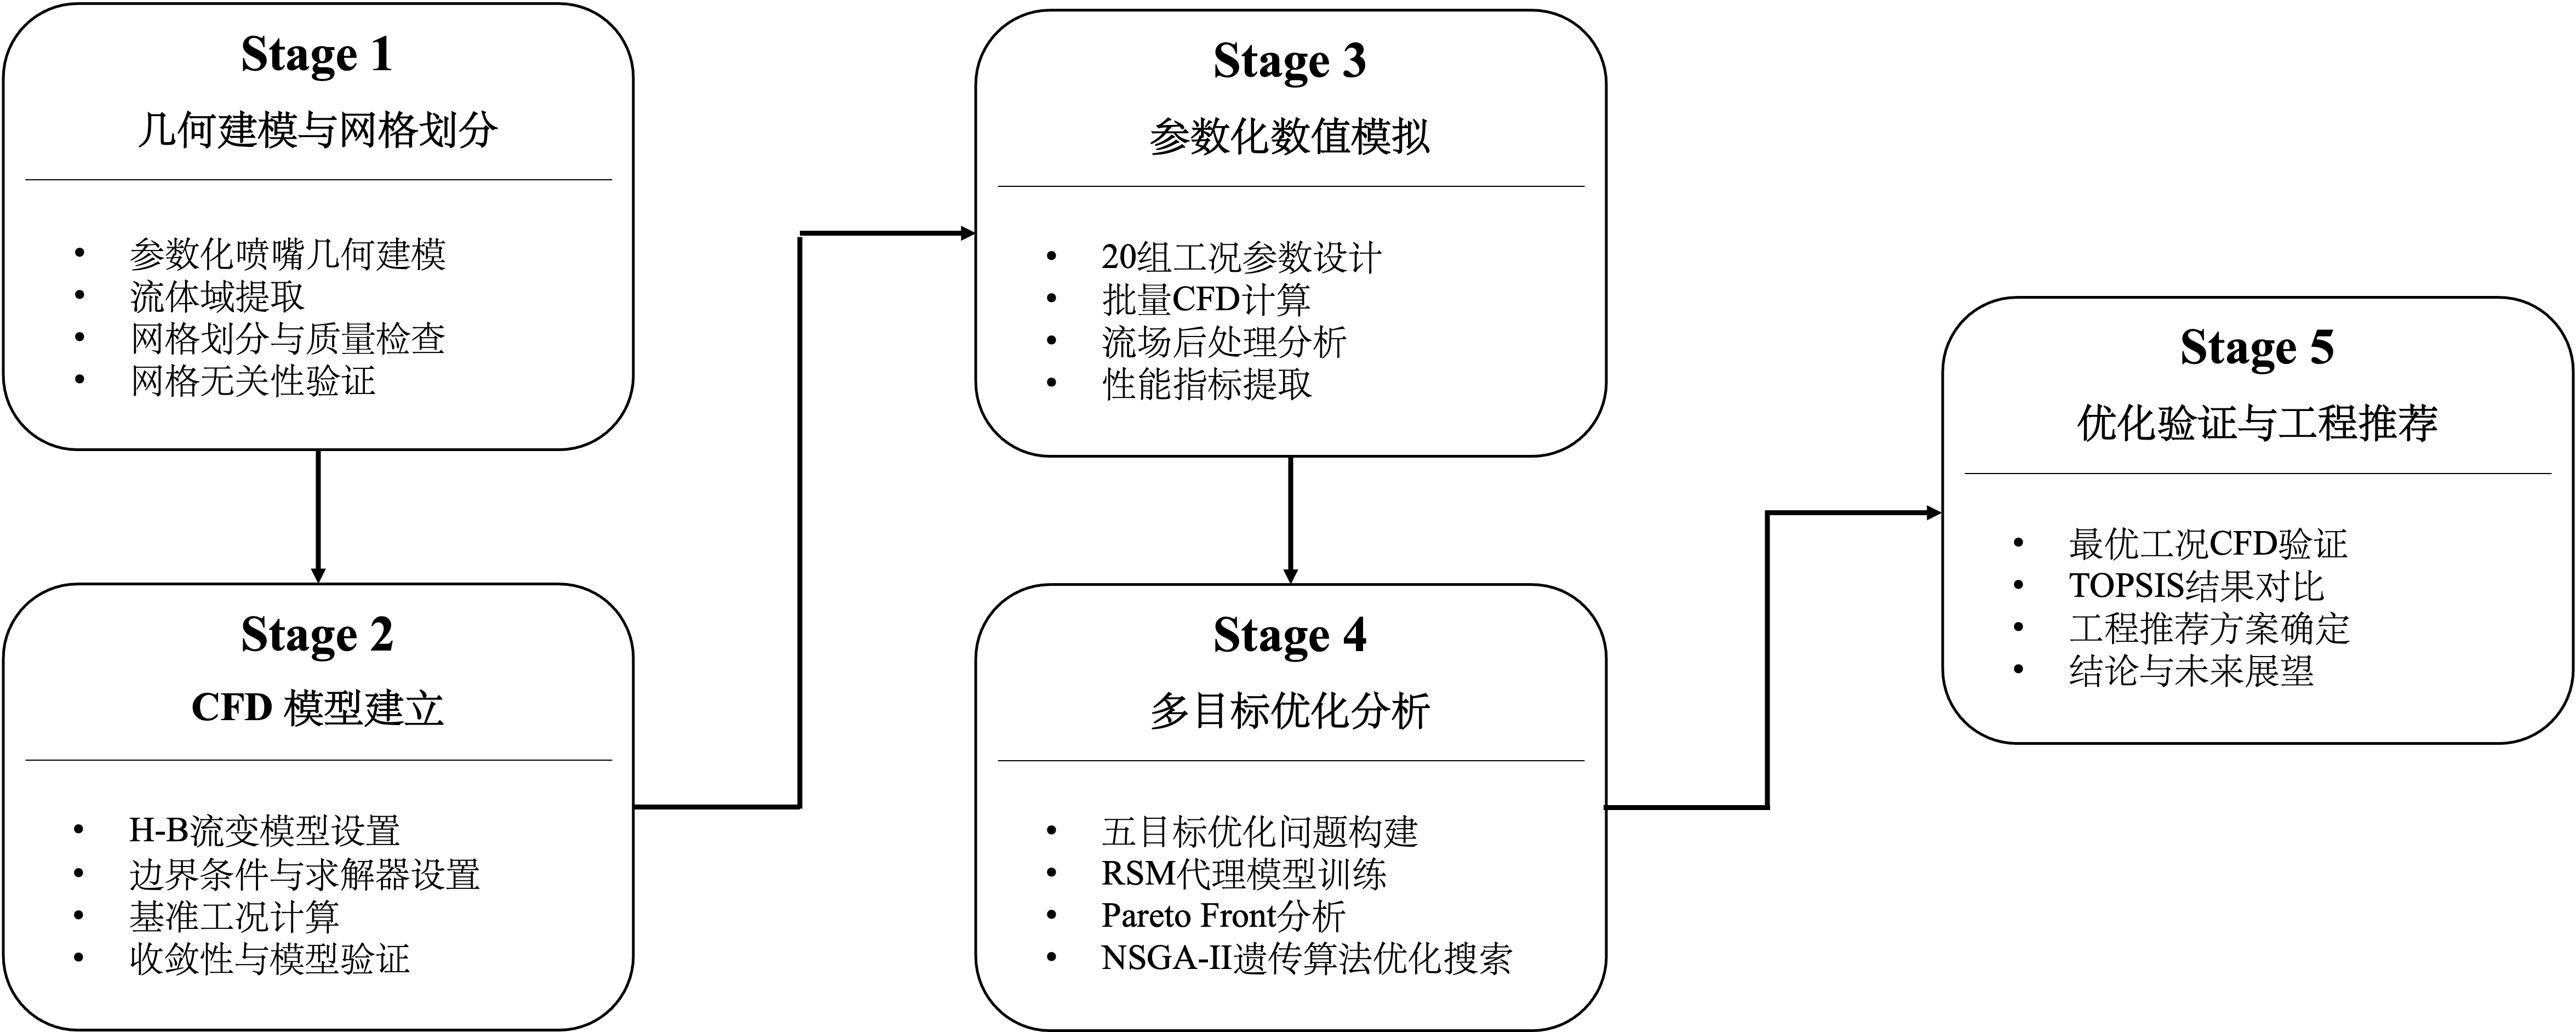
\includegraphics[width=0.9\textwidth]{figures/1.1.png}
  \caption{技术路线流程图}
  \label{fig:1.1}
\end{figure}

\chapter{数值模型建立与验证}\label{chap:model}

\section{物理问题描述与几何模型}

\subsection{打印系统几何构型}

本论文的研究对象为一种带有整形板结构的挤出式三维混凝土打印（3D Concrete Printing, 3DCP）喷嘴组合体，其整体结构主要由喷嘴主体与后置整形板两部分组成。该结构旨在模拟打印混凝土在实际挤出沉积过程中的流动、压实与成形行为，并研究不同几何参数对打印质量与流场特性的影响规律。

喷嘴主体由竖直圆柱形入口直管、锥形收缩段以及出口直管段组成。喷嘴入口直管长度（Straight Tube Length）为100~mm，用于保证浆体在进入收缩区域前形成相对稳定的流动状态。锥形收缩段（竖向长度L、半锥角$\theta$）对混凝土浆体进行渐缩加压，使流体由较大截面逐渐过渡至出口区域，进一步稳定出口流场并控制挤出过程中的速度分布。

整形板结构安装于喷嘴出口下方，主要由顶部水平板、前挡板、左右侧板以及倾斜出料段组成。左右侧板厚度均为11~mm，用于限制打印材料横向扩散。整形板倾斜出料段长度记为TL，倾角记为$\alpha$。整形板的主要功能是在混凝土挤出后对其进行二次压实与几何整形，以改善打印层的表面平整度、层间接触质量以及截面一致性。喷嘴出口底面与基底面之间的垂直距离定义为$Z_0$。本研究中限制$Z_0 = 22$~mm，以保证混凝土打印层高的可用性与CFD建模结果的可对比性。

打印过程中，混凝土材料经喷嘴挤出后，其最终形成的打印层高度$H$不仅受到喷嘴出口高度的影响，还与整形板倾斜出料段的几何参数密切相关。根据几何关系，打印层高度可表示为：
\begin{equation}\label{eq:H}
  H = Z_0 - TL \cdot \sin(\alpha).
\end{equation}
由此进一步可得打印层高度对倾角$\alpha$的偏导关系为：
\begin{equation}\label{eq:dH-dalpha}
  \frac{\partial H}{\partial \alpha} = -TL \cos(\alpha) < 0.
\end{equation}
由\cref{eq:dH-dalpha}可知，在TL保持不变的条件下，随着整形板倾角$\alpha$增大，打印层高度$H$将逐渐减小，即整形板对材料的压实作用增强。这表明整形板几何参数会直接影响打印层的压实程度与沉积形态，是本课题的研究重点之一。

考虑到实际3D打印混凝土施工中，不同打印对象对于层高具有不同要求，本研究参考现有打印工艺范围，将打印层高度的研究边界设定为：
\begin{equation}\label{eq:H-range}
  5~\text{mm} \leq H \leq 20~\text{mm}.
\end{equation}
该范围能够覆盖大多数挤出式混凝土打印的典型层高条件，同时兼顾打印稳定性与结构成形质量。

组合体几何模型的三维结构示意图以及主要几何参数定义的侧视剖面图分别如\cref{fig:2.1}与\cref{fig:2.2}所示。

\begin{figure}[!htb]
  \centering
  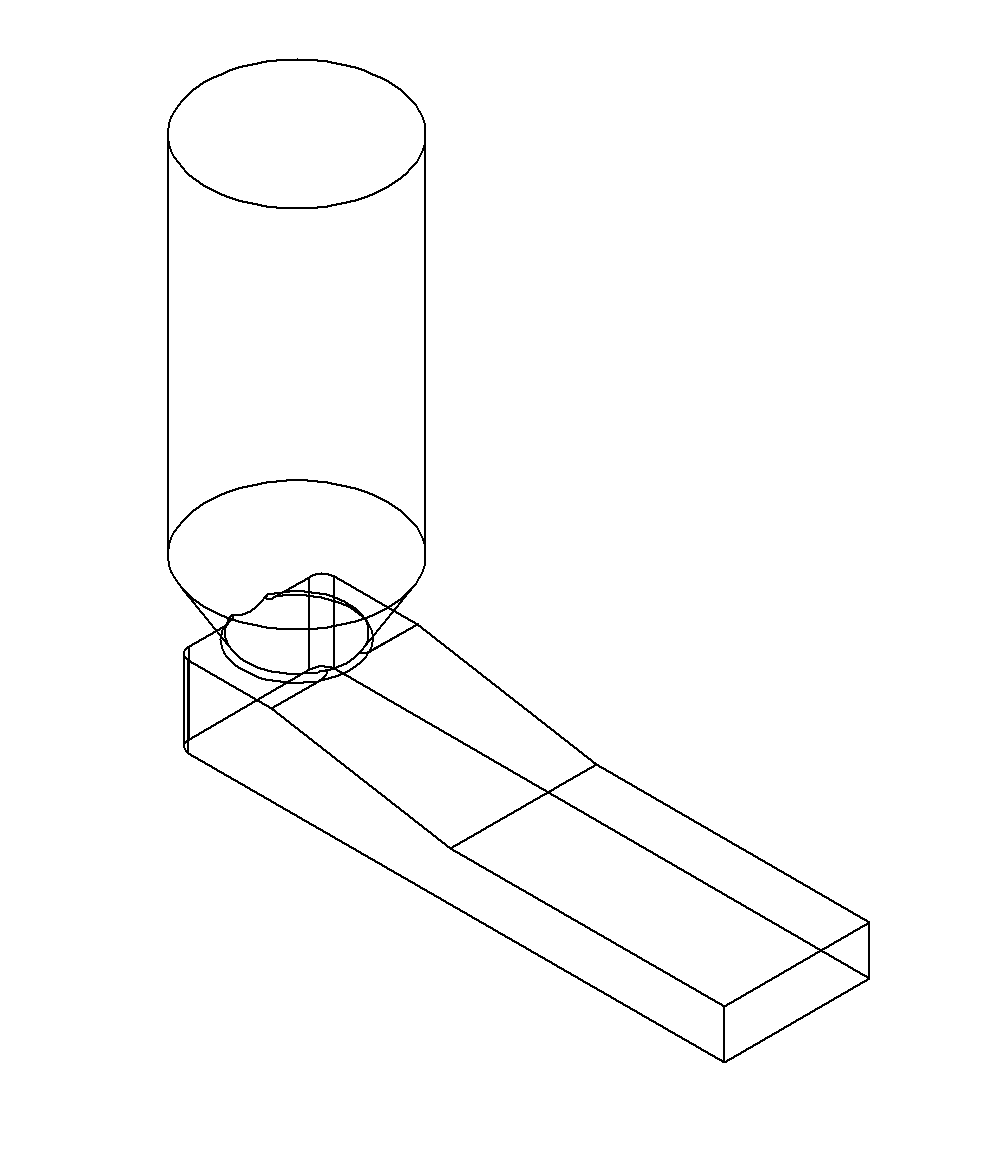
\includegraphics[width=0.7\textwidth]{figures/2.1.PNG}
  \caption{几何模型三维示意图}
  \label{fig:2.1}
\end{figure}

\begin{figure}[!htb]
  \centering
  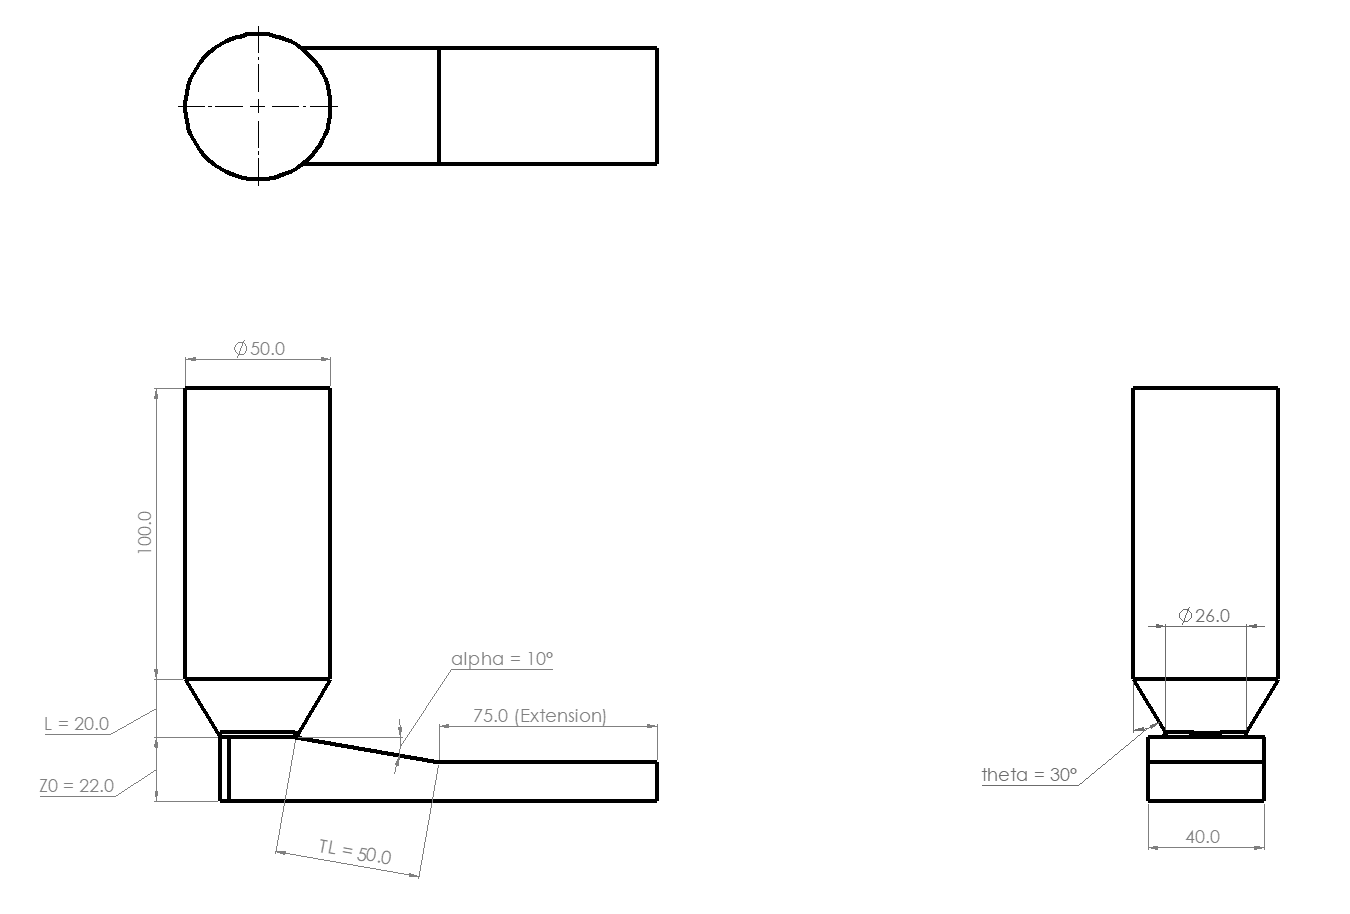
\includegraphics[width=0.7\textwidth]{figures/2.2.png}
  \caption{几何参数定义侧视剖面图}
  \label{fig:2.2}
\end{figure}

为研究喷嘴与整形板结构参数对打印流场及成形性能的影响规律，本文选取四个关键几何参数作为主要研究变量：锥形收缩段半锥角$\theta$、喷嘴竖直长度L、整形板倾斜出料段长度TL以及倾斜角$\alpha$。研究重点分析上述参数对基底接触压力（Substrate Pressure）、剪切应力（Shear Stress）以及压力传递效率（Pressure Transfer Efficiency）等指标的影响机制。除上述变量外，其余结构参数均采用He等\cite{he2024}中所提出的标准尺寸，以保证模型具有一定的工程参考价值与对比一致性。

各参数组合与对应工况汇总如\cref{tab:2.1}所示。

\begin{table}[!htb]
  \centering
  \caption{几何参数定义与基准值汇总}\label{tab:2.1}
  \renewcommand{\arraystretch}{1.3}
  \begin{tabular}{cclc}
    \toprule
    \textbf{参数} & \textbf{符号} & \textbf{基准值} & \textbf{变化范围} \\
    \midrule
    入口直径   & $D_{in}$  & 47 mm & 固定（由$\theta$、L、$D_{out}$决定） \\
    出口直径   & $D_{out}$ & 26 mm & 固定 \\
    收缩角     & $\theta$  & 30°   & 0°, 15°, 30°, 45°, 60° \\
    直管段长   & $L$       & 20 mm & 10, 20, 30, 40 mm \\
    整形板长   & $TL$      & 50 mm & 30, 40, 50, 55, 60, 70 mm \\
    倾斜角     & $\alpha$  & 10°   & 0°, 5°, 10°, 15°, 20° \\
    出口距基底 & $Z_0$     & 22 mm & 固定 \\
    侧板/前板厚 & $t$      & 11 mm & 固定 \\
    \bottomrule
  \end{tabular}
\end{table}

\subsection{坐标系与边界面定义}

为便于对打印混凝土在喷嘴及整形板内部的流动行为进行分析，并统一后续压力、速度及剪切应力等物理量的方向定义，本课题建立三维直角坐标系对计算域进行描述。其中，Y轴定义为竖直方向，正方向向上；X轴定义为打印方向，即混凝土材料沿整形板延伸方向的运动方向；Z轴定义为横向方向，用于描述打印层宽度方向上的流动特征。重力加速度$g$沿Y轴负方向施加，其取值为：
\begin{equation}\label{eq:gravity}
  g = -9.81~\text{m/s}^2,
\end{equation}
用于模拟实际打印过程中混凝土浆体在自重作用下的流动与沉积行为。

为定量分析流场内部不同区域的流动特征，本课题在模型中设置了多个监测边界面与特征截面，以便后续提取压力、速度、剪切应力及质量流量等关键参数。各边界面定义如下：

（1）Inlet（喷嘴入口顶面）：Inlet为喷嘴入口顶面，其法向方向垂直于Y轴，用于施加入口边界条件，包括入口速度、体积流量及材料流变参数等。

（2）Nozzle Outlet Plane（喷嘴出口截面）：Nozzle Outlet Plane为喷嘴出口截面，其法向方向同样垂直于Y轴。该截面用于分析混凝土材料在离开喷嘴瞬间的速度分布、静压力分布及流场均匀性，是研究喷嘴内部压力传递行为的重要监测位置。

（3）Trowel Outlet Plane（出料口截面）：Trowel Outlet Plane为整形板倾斜出料段末端截面，其法向方向垂直于X轴。该截面主要用于研究整形板对材料流动状态及截面形状的整形作用，并用于评估挤出后材料的速度稳定性与压实效果。

（4）Outlet（延伸段边界面）：Outlet为计算域末端延伸段出口边界，其法向方向垂直于X轴。该边界用于保证流场出口区域具有充分发展长度，从而减小出口边界条件对主流场计算结果的影响。

（5）Substrate（打印基底面）：Substrate为打印基底面，其平面方向平行于XZ平面，用于模拟实际打印过程中的基板接触界面。该区域是研究基底接触压力、剪切应力以及层间压实行为的关键监测区域。

（6）Wall（外部壁面）：Wall是所有在混凝土挤出过程中对流体施加空间边界条件的面，由喷嘴直管壁面、喷嘴收缩段壁面、整形板上顶面、整形板前、左、右壁面共同组成。

上述边界面的空间位置关系如\cref{fig:2.3}所示。

\begin{figure}[!htb]
  \centering
  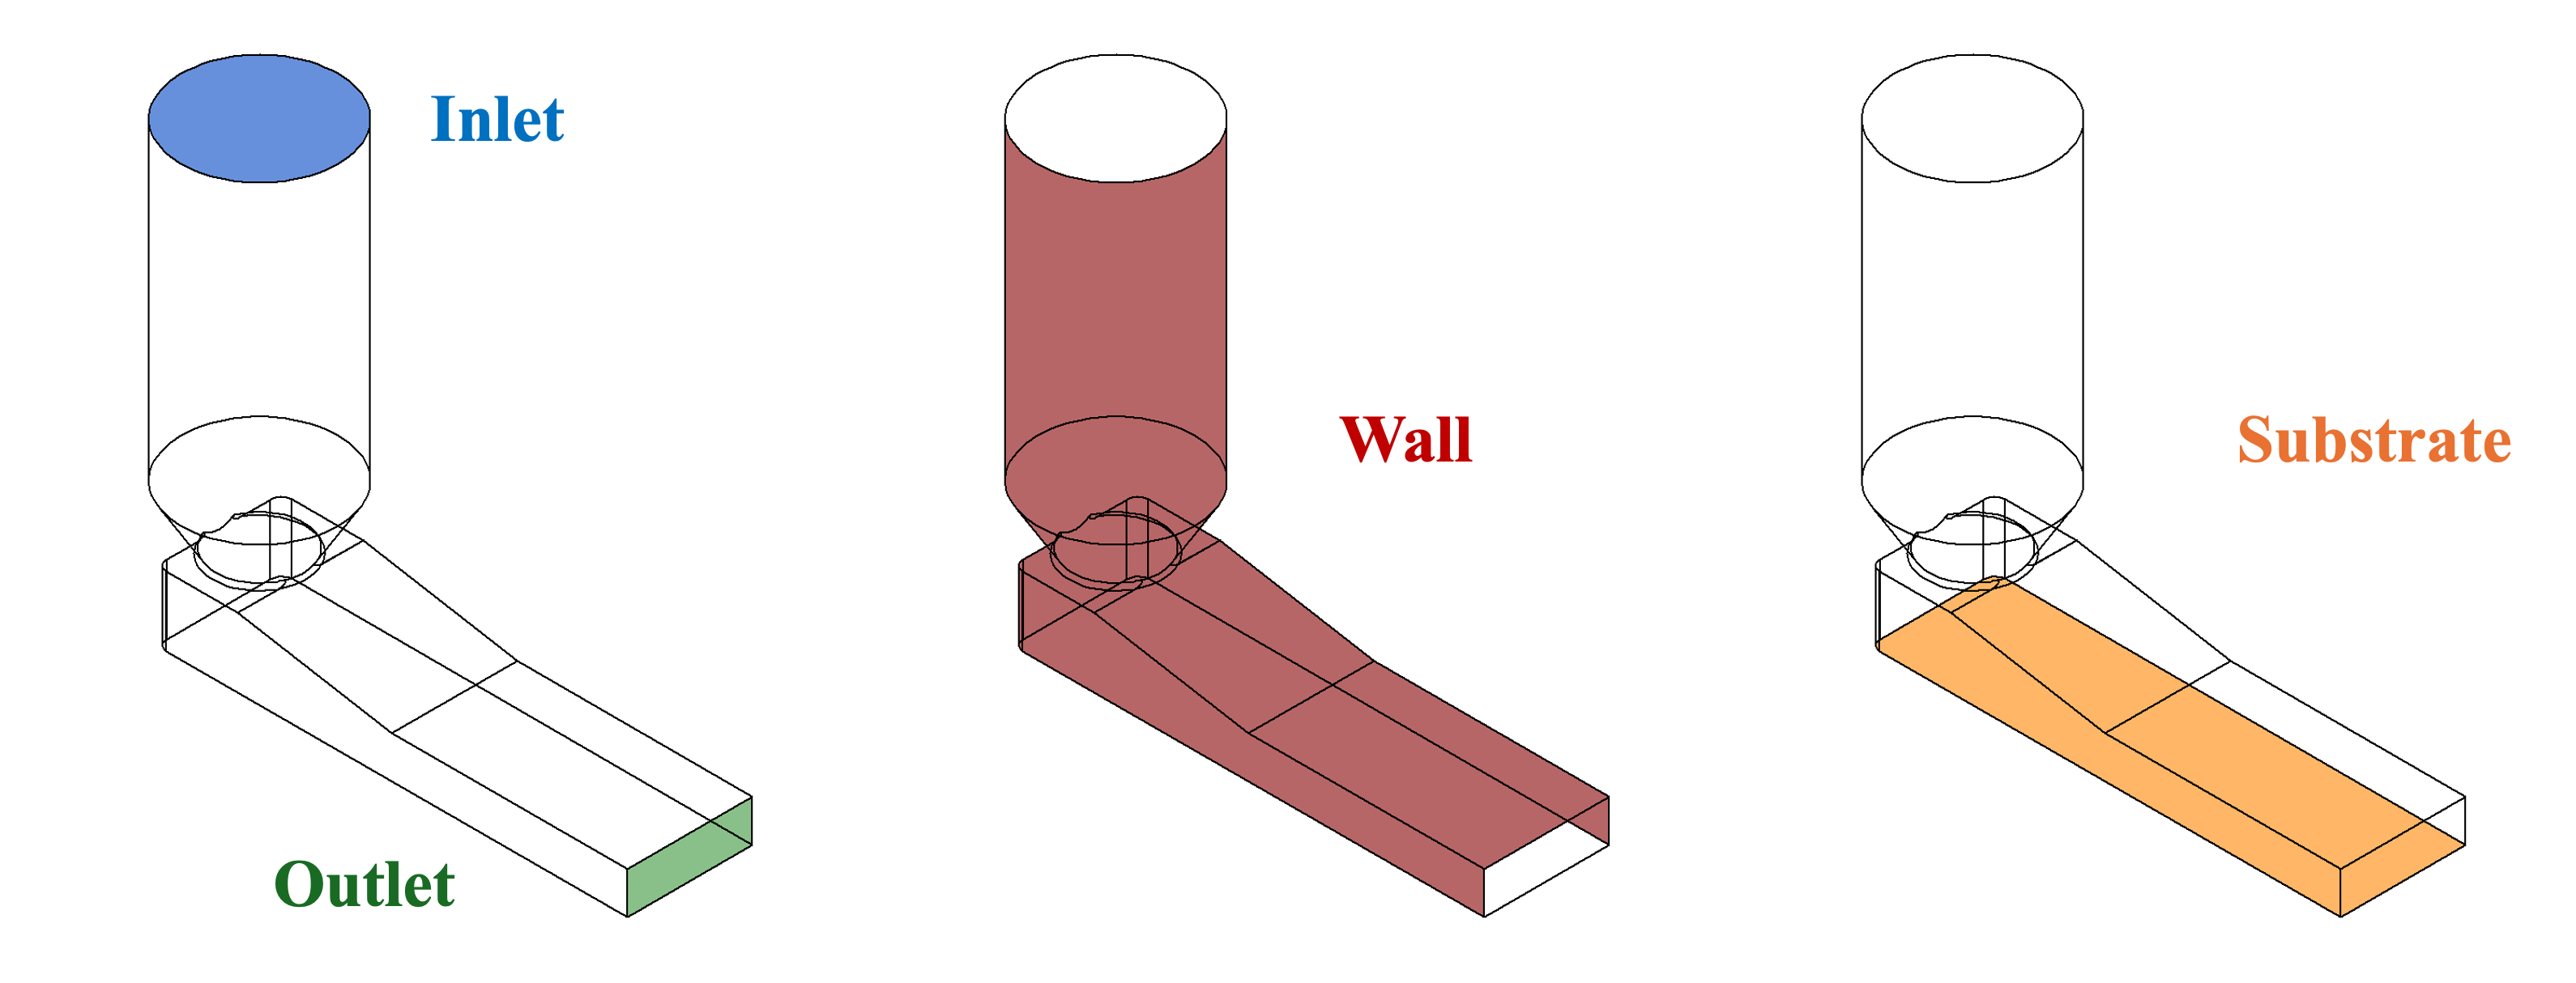
\includegraphics[width=0.7\textwidth]{figures/2.3.png}
  \caption{边界条件分布示意图}
  \label{fig:2.3}
\end{figure}

\section{控制方程与本构模型}

\subsection{连续方程与动量方程}

为描述打印混凝土浆体在喷嘴内部及整形板区域的流动行为，本文基于计算流体动力学（CFD）建立控制方程。考虑到打印过程中温度变化较小，且浆体流动速度较低，本文将打印混凝土浆体假设为等温、单相、不可压缩稳态非牛顿流体，并忽略材料离析及气泡对流场的影响。

在上述假设条件下，浆体流动满足质量守恒方程与动量守恒方程。不可压缩流体的连续性方程表示为：
\begin{equation}\label{eq:continuity}
  \nabla \cdot \mathbf{u} = 0,
\end{equation}
其中，$\mathbf{u}$是速度矢量。

浆体流动的动量守恒方程采用Navier--Stokes方程表示：
\begin{equation}\label{eq:NS}
  \rho (\mathbf{u} \cdot \nabla) \mathbf{u} = -\nabla p + \nabla \cdot \left[ \eta(\dot{\gamma}) \cdot (\nabla \mathbf{u} + (\nabla \mathbf{u})^T) \right] + \rho \mathbf{g},
\end{equation}
其中，$\rho$为浆体密度（2100~kg/m³），$p$为静压力，$\eta$为黏性应力张量，$\mathbf{g}$为重力加速度矢量（$\mathbf{g} = -9.81 \hat{\mathbf{j}}$~m/s²）；$\eta(\dot{\gamma})$为依赖于局部剪切速率$\dot{\gamma}$的表观黏度，由Herschel--Bulkley本构模型描述。由于打印混凝土浆体在喷嘴内的广义雷诺数$Re_{gen} \approx 0.007 \ll 1$，对流惯性项$\rho(\mathbf{u} \cdot \nabla)\mathbf{u}$远小于黏性项，流动处于蠕动流（Stokes flow）范畴，黏性力主导流场行为。

\subsection{Herschel-Bulkley本构模型}

为更加准确地描述打印混凝土浆体的非牛顿流变特性，本课题采用Herschel-Bulkley（H-B）本构模型对浆体的黏塑性行为进行表征，而未采用传统Bingham模型。相比于Bingham模型，H-B模型能够同时反映材料的屈服应力特性以及剪切变稀行为，更适用于打印混凝土在挤出过程中的复杂流动状态。

Herschel-Bulkley本构模型表示为：
\begin{equation}\label{eq:HB}
  \eta(\dot{\gamma}) = \begin{cases}
    \dfrac{\tau_0}{\dot{\gamma}} + k \dot{\gamma}^{n-1}, & \dot{\gamma} > \dot{\gamma}_c, \\[6pt]
    \dfrac{\tau_0}{\dot{\gamma}_c} + k \dot{\gamma}^{n-1}, & \dot{\gamma} \leq \dot{\gamma}_c,
  \end{cases}
\end{equation}
式中，$\tau_0$为屈服应力（Pa），表征材料开始流动所需克服的最小剪切应力；$k$为稠度系数（$\text{Pa} \cdot \text{s}^n$），反映材料整体黏度水平；$n$为流动指数（无量纲），当$n < 1$时材料表现为剪切变稀行为，当$n = 1$时H-B模型退化为Bingham模型；$\dot{\gamma}_c$为截断剪切速率。H-B模型在低剪切速率区域可能出现表观黏度趋于无穷大的数值问题，$\dot{\gamma}_c$的引入对模型进行Papanastasiou正则化，可提高数值计算稳定性，也可以有效避免低剪切速率区域黏度奇异性。

本文所用各流变参数取值参考已有文献中典型打印混凝土的测量结果，具体见\cref{tab:2.2}。模型对应的黏度-剪切速率关系曲线如\cref{fig:2.4}所示。

\begin{table}[!htb]
  \centering
  \caption{H-B流变参数取值及文献依据}\label{tab:2.2}
  \renewcommand{\arraystretch}{1.3}
  \begin{tabular}{clcl}
    \toprule
    \textbf{参数} & \textbf{符号} & \textbf{取值} & \textbf{物理意义与文献依据} \\
    \midrule
    屈服应力      & $\tau_0$         & 500 Pa            & 材料静止承载能力；参考He\cite{he2024}, Chen\cite{chen2020} \\
    稠度系数      & $k$              & 15 Pa·sⁿ          & 整体黏度水平 \\
    流动指数      & $n$              & 0.45              & 剪切变稀程度（$n<1$）；参考文献取值范围0.3-0.6 \\
    截断剪切速率  & $\dot{\gamma}_c$ & 0.01 s⁻¹          & Papanastasiou正则化截断点 \\
    最大黏度      & $\eta_{max}$     & 50000 Pa·s        & 未屈服区上限 \\
    最小黏度      & $\eta_{min}$     & 1 Pa·s            & 数值稳定下限 \\
    材料密度      & $\rho$           & 2100 kg/m³        & 典型水泥砂浆密度 \\
    \bottomrule
  \end{tabular}
\end{table}

\begin{figure}[!htb]
  \centering
  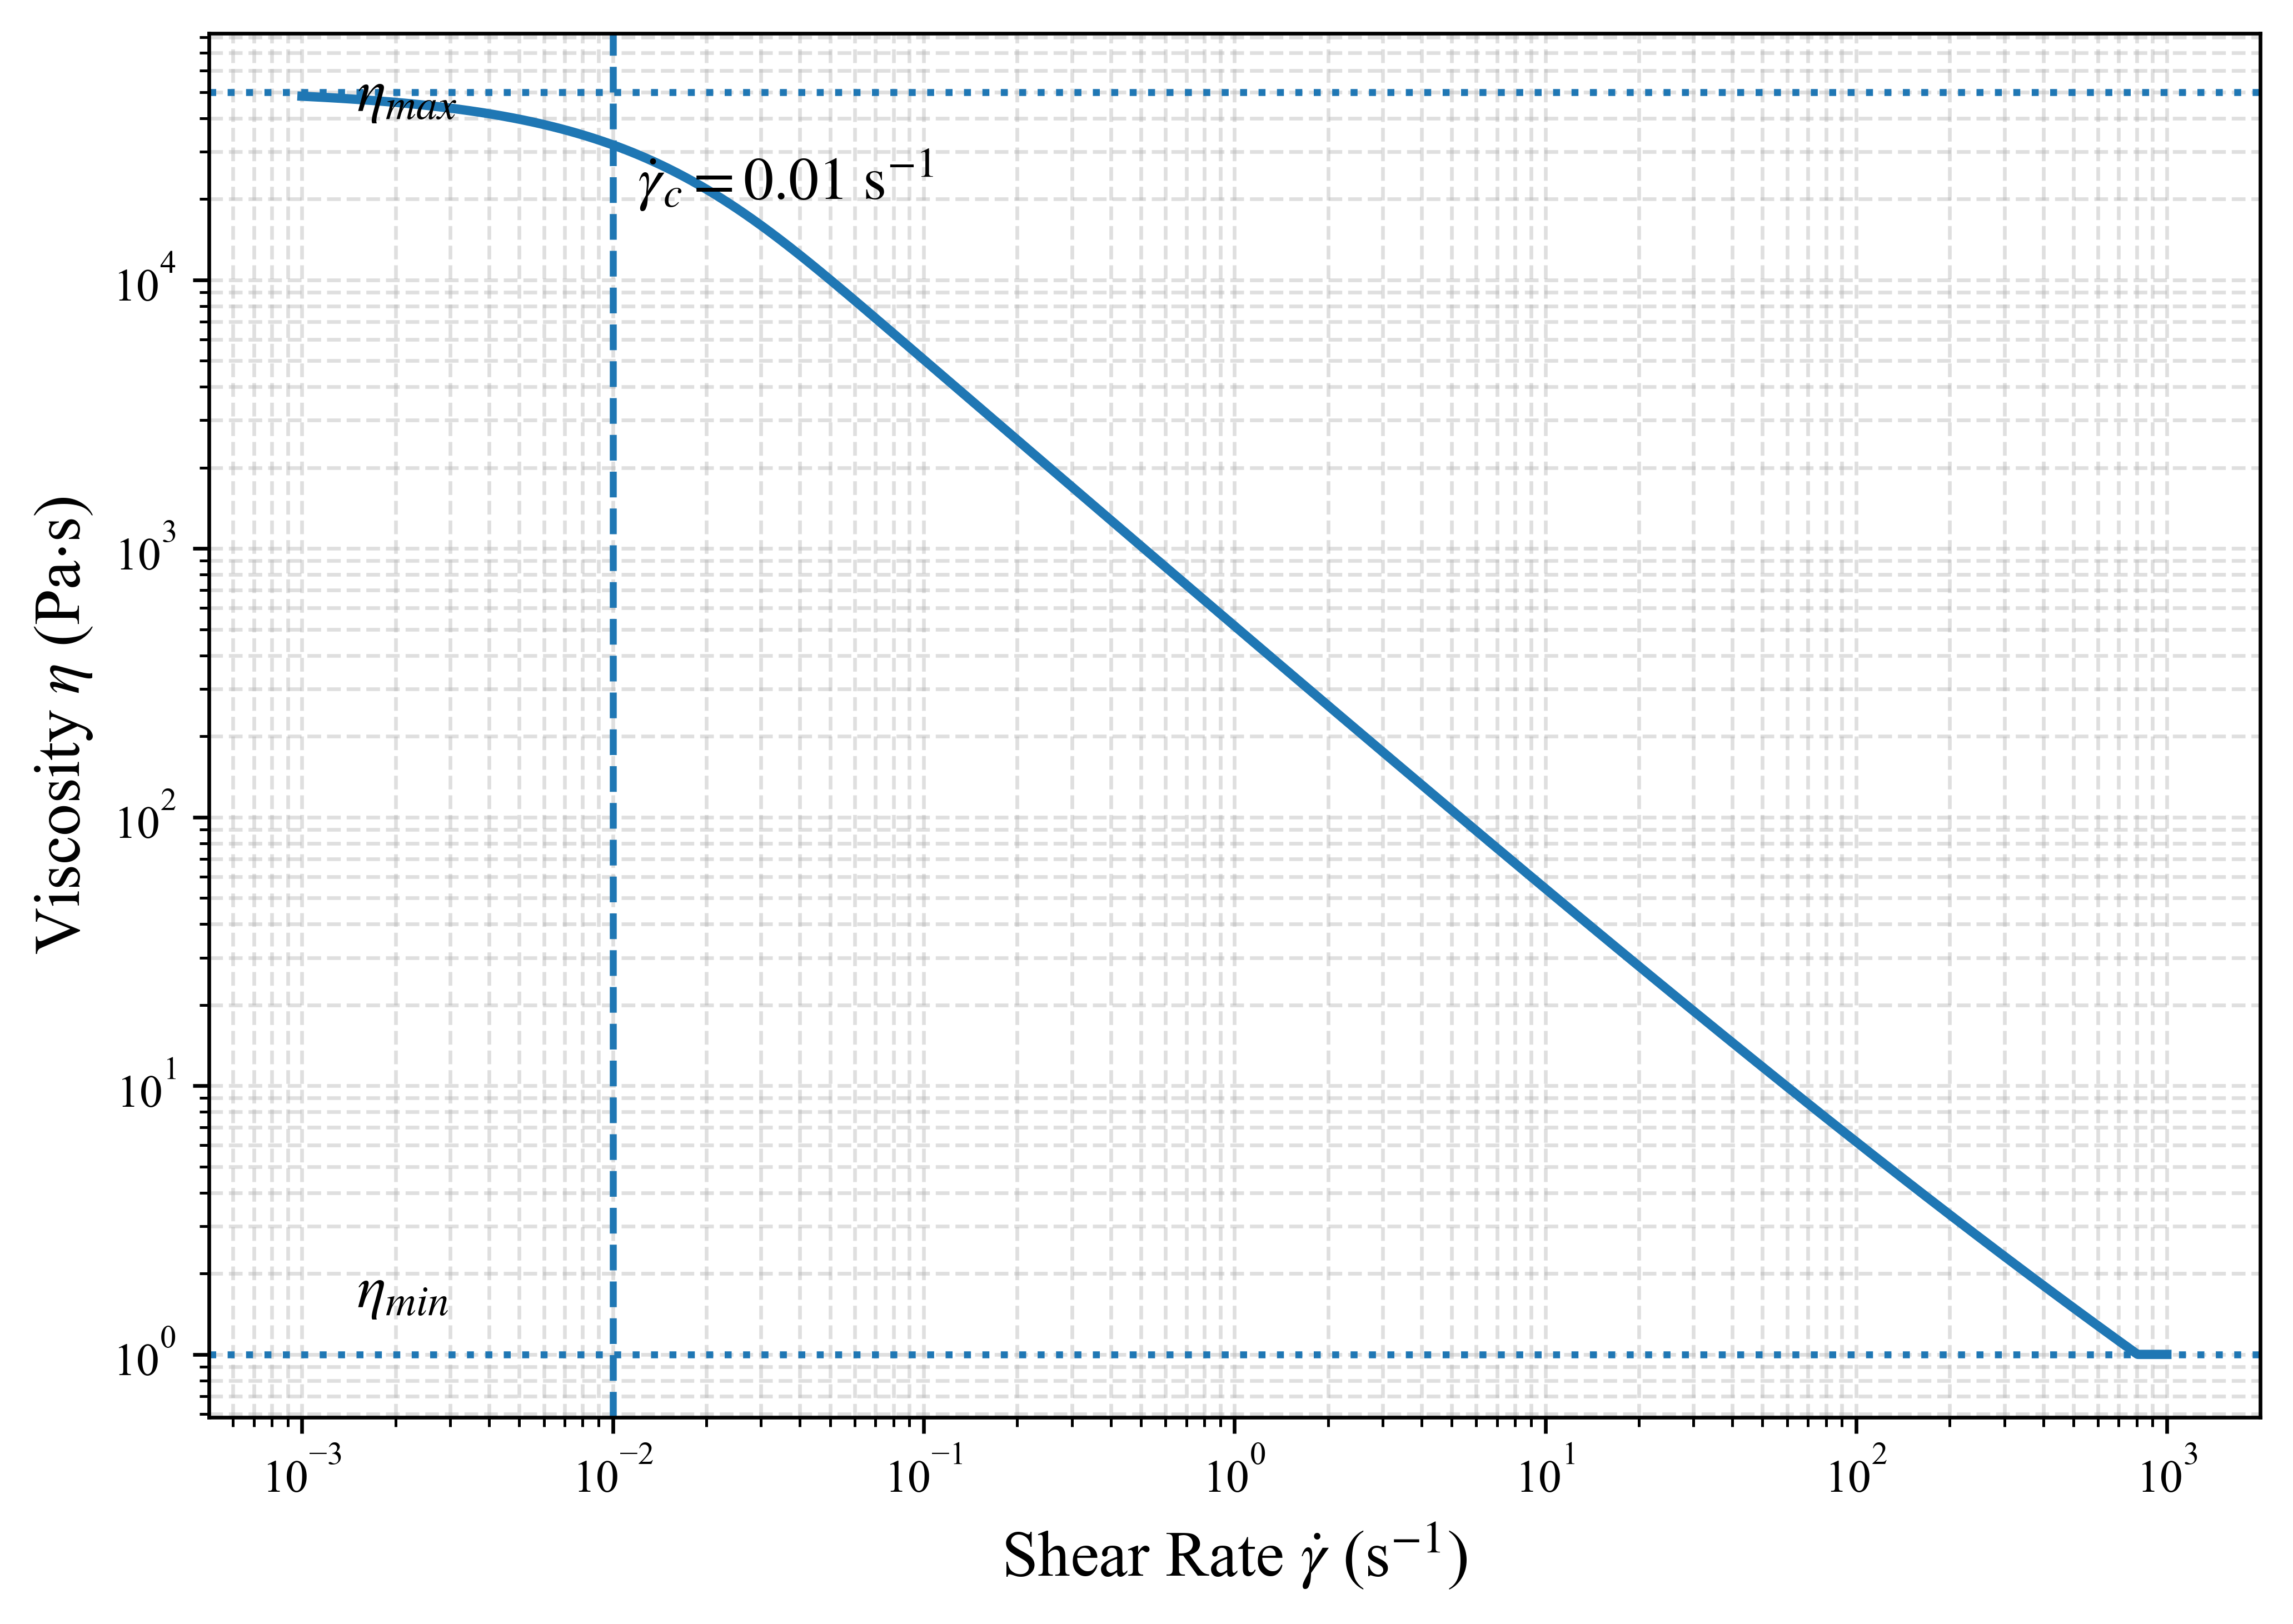
\includegraphics[width=0.7\textwidth]{figures/2.4.png}
  \caption{H-B模型黏度--剪切速率曲线}
  \label{fig:2.4}
\end{figure}

\subsection{雷诺数估算与层流假设验证}

在基准工况（见\cref{chap:baseline}第\ref{sec:baseline-params}节）下，喷嘴出口处典型剪切速率为：
\begin{equation}\label{eq:gamma-typ}
  \dot{\gamma} \approx \frac{v_{in}}{R} \approx \frac{0.03}{0.013} \approx 2.3~\text{s}^{-1}.
\end{equation}
对应有效黏度为：
\begin{equation}\label{eq:eta-eff}
  \eta_{eff} \approx \frac{\tau_0}{\dot{\gamma}} + k \cdot \dot{\gamma}^{n-1} = \frac{500}{2.3} + 15 \times 2.3^{-0.55} \approx 227~\text{Pa} \cdot \text{s}.
\end{equation}
广义雷诺数为：
\begin{equation}\label{eq:Re}
  Re_{general} = \frac{\rho v D}{\eta_{eff}} = \frac{2100 \times 0.03 \times 0.026}{227} \approx 0.0072 \ll 1.
\end{equation}
由以上计算可见，混凝土浆体的广义雷诺数$Re_{general}$远小于1，证明层流假设成立。

\section{计算域离散与网格划分}

\subsection{几何建模与流体域提取}

本课题采用SolidWorks 2024软件建立喷嘴组合体三维几何模型。为实现不同工况下几何参数的快速调整与批量建模，模型构建过程中采用Equation参数化驱动方式，对各草图（Sketch）的关键尺寸进行统一控制，从而实现喷嘴半锥角$\theta$、出口直管长度$L$、整形板长度$TL$及倾角$\alpha$等参数的参数化建模。

完成实体建模后，采用Cavity命令提取组合体内部流体域，以构建后续CFD计算所需的流体计算区域。为提高数值计算稳定性并减小边界条件对主流场的影响，本课题进一步对流体域进行了两部分延伸处理：

（1）在整形板出料口末端沿材料挤出方向增加75~mm自由延伸段，用于模拟浆体离开整形板后的自由流动区域；

（2）保留整形板底部至打印基底面之间的悬空区域，用于描述浆体与基底接触前后的流动与压实行为。

最终建立的流体域主要包括喷嘴入口直管段、锥形收缩段、出口直管段、整形板受限流动区域（由顶部板与侧板围成）以及自由延伸段。

流体域模型导出后，在ANSYS SpaceClaim中对各边界面按照计算规则进行命名，并对几何体封闭性与拓扑连续性进行检查，以保证后续网格划分与数值计算的正确性。

\subsection{网格策略}

本研究采用非结构化四面体网格对流体域进行离散化处理，以平衡计算效率与几何适应性。全局尺寸定义为每个流体域推荐的网格尺寸，以避免对模型的过度复杂化。

为精确捕捉关键区域的流动细节，对喷嘴入口、整形板出口及其接触的圆弧面实施了边缘局部加密策略，确保相关边缘网格尺寸细化至0.5~mm-1~mm。同时，在所有固壁面设置了包含5层单元、增长比为1.2的Inflation边界层，以保障近壁面流动的解析精度。\cref{fig:2.5}与\cref{fig:2.6}分别展示了基础工况的整体网格示意图及喷嘴收缩段与整形板受限区的局部加密细节。

\begin{figure}[!htb]
  \centering
  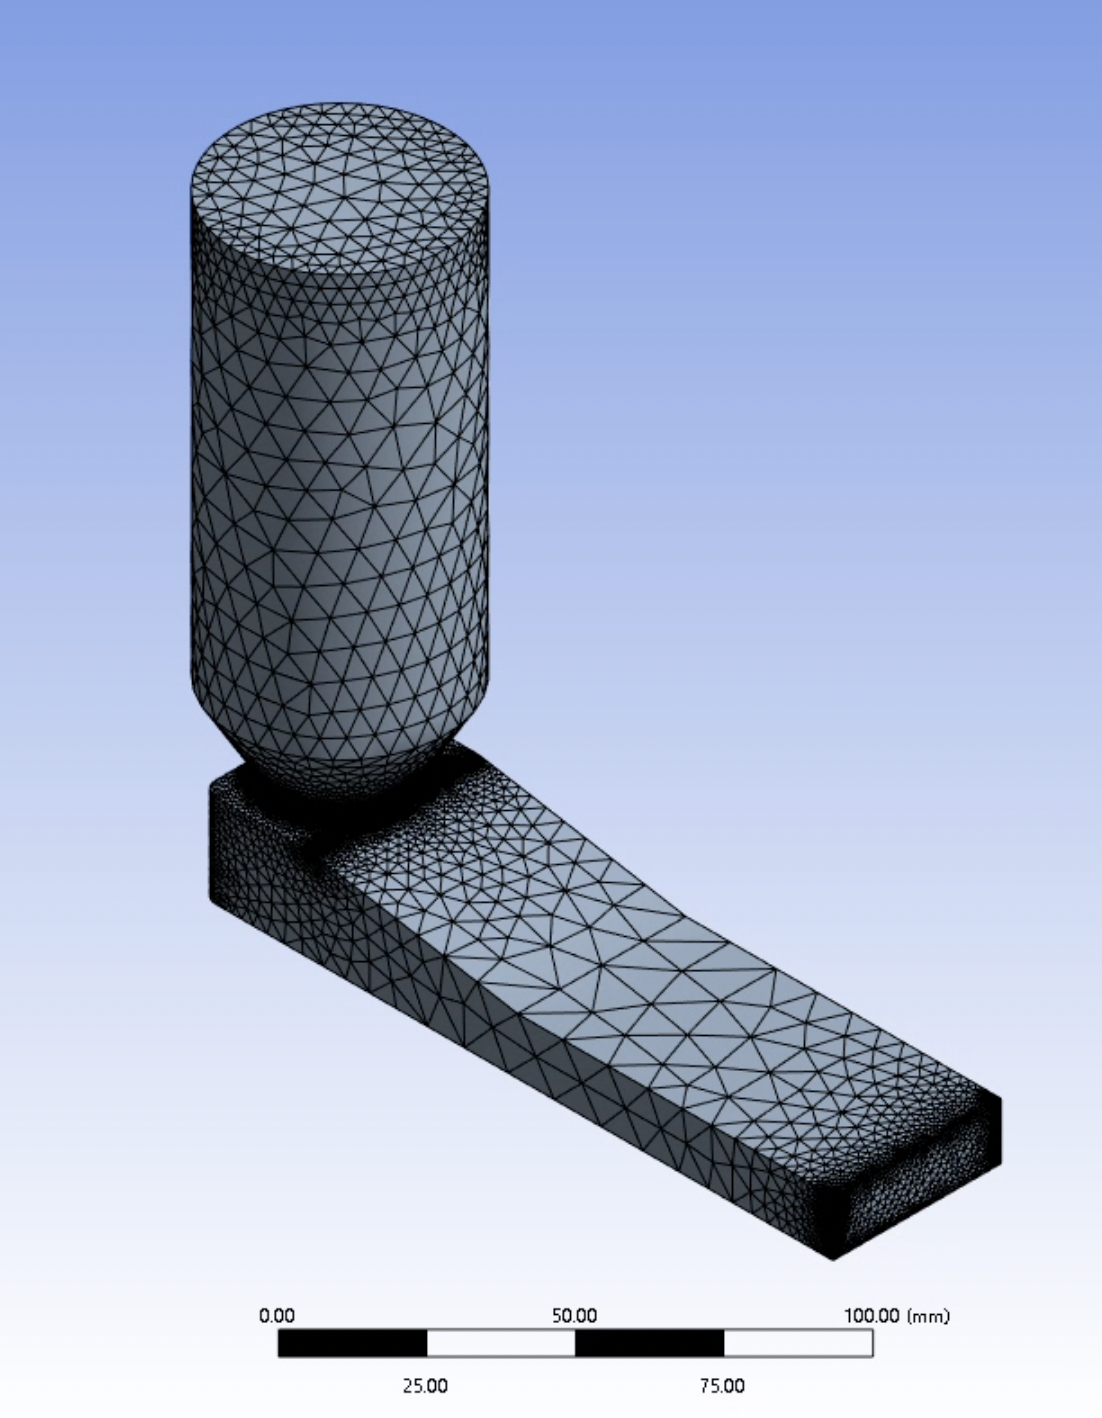
\includegraphics[width=0.7\textwidth]{figures/2.5.png}
  \caption{整体网格示意图（Baseline工况）}
  \label{fig:2.5}
\end{figure}

\begin{figure}[!htb]
  \centering
  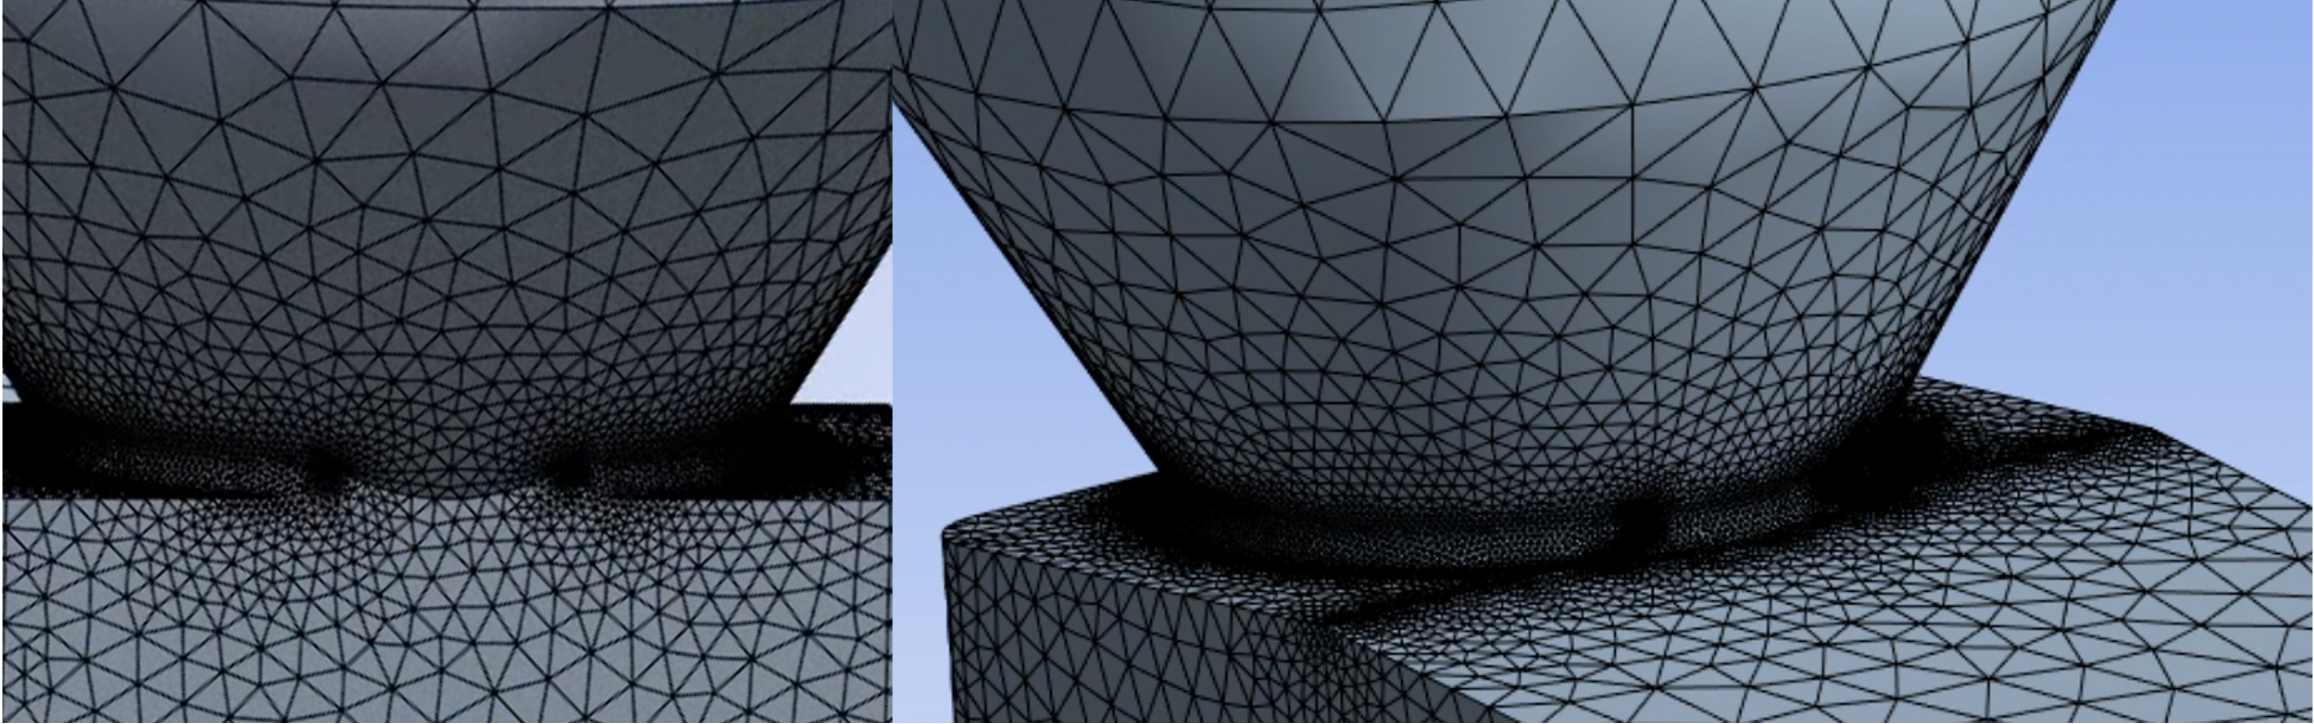
\includegraphics[width=0.7\textwidth]{figures/2.6.png}
  \caption{喷嘴收缩段与整形板受限区局部加密细节图}
  \label{fig:2.6}
\end{figure}

\subsection{网格质量评估}

\cref{tab:2.3}列出了代表性工况的网格质量评价结果。各工况网格均满足CFD数值计算对网格质量的基本要求，能够保证求解过程的稳定性与计算结果的可靠性。

针对NSGA-II优化验证工况（见\cref{chap:optimization}第\ref{sec:nsga2}节），进一步对网格切向偏斜度（Tangent Skewness）进行了检查，其最大值为3.25，仍处于可接受范围内，表明网格质量能够满足复杂流场条件下的数值模拟需求。

\begin{table}[!htb]
  \centering
  \caption{各代表性工况网格质量汇总}\label{tab:2.3}
  \renewcommand{\arraystretch}{1.3}
  \begin{tabular}{cccccp{2.5cm}}
    \toprule
    \textbf{工况} & \textbf{最大面面积} & \textbf{最小单元体积} & \textbf{最小正交性质量} & \textbf{最大长宽比} & \textbf{备注} \\
    \midrule
    Baseline       & 7.77E-05 & 6.12E-14 & 0.202 & 14.92 & 代表性工况 \\
    A1-4           & 1.37E-04 & 8.15E-14 & 0.177 & 17.03 & 收缩段最大 \\
    C3             & 1.18E-04 & 9.53E-15 & 0.204 & 16.29 & 最优工况 \\
    Pareto Optimum & 2.16E-04 & 2.98E-14 & 0.202 & 16.63 & Skewness=3.25 \\
    \bottomrule
  \end{tabular}
  \vspace{0.5em}
  
  \footnotesize{*其余工况均满足Min Orth.Q $>0.17$, Max AR $<18$。}
\end{table}

\subsection{网格无关性验证}

为评估数值结果对网格密度的敏感性并确定满足精度要求的最优网格方案，本文以C3工况（$\theta = 60°$，$L = 20$~mm，$TL = 60$~mm，$\alpha = 15°$，含边角圆滑处理）为验证对象，系统开展网格无关性研究。C3工况几何复杂度最高（含喷嘴收缩段、整形板倾斜面与圆角过渡区），对网格质量的要求最为严苛，将其作为验证工况具有代表性，可覆盖本研究全部工况。

网格无关性验证选取基底面（Substrate）的面积加权平均静压力$P_{sub,AWA}$作为网格无关性监测量。该指标为本研究的核心评价目标，对流场细节（尤其是整形板约束区近壁速度梯度与压力分布）最为敏感，适合作为网格收敛性的判别基准。

实验共设置五组全局网格尺寸：12.9~mm（粗）、8~mm、5~mm、3~mm和1~mm，在保持边界层Inflation设置（5层，增长比1.2）和关键区域局部加密策略不变的前提下，仅系统改变全局网格尺寸。各组网格统计数据与监测量结果汇总于\cref{tab:2.4}。

\begin{table}[!htb]
  \centering
  \caption{网格无关性验证数据（C3工况）}\label{tab:2.4}
  \renewcommand{\arraystretch}{1.3}
  \begin{tabular}{ccccl}
    \toprule
    \textbf{网格尺寸} & \textbf{最大长宽比} & $P_{sub,AWA}$ \textbf{(Pa)} & \textbf{与3 mm误差(\%)} & \textbf{评级} \\
    \midrule
    12.9 mm（粗）     & 16.2866 & 21702 & 2.5\% & 粗网格，通过 \\
    8 mm              & 17.3505 & 21503 & 3.5\% & 合格 \\
    5 mm              & 16.5882 & 22090 & 0.8\% & 推荐网格 \\
    3 mm（基准）       & 15.4398 & 22273 & ---    & 参考基准 \\
    1 mm              & 17.9311 & 22579 & 1.4\% & 曲面振荡，不采用 \\
    \bottomrule
  \end{tabular}
\end{table}

收敛性分析结果如\cref{fig:2.7}所示。

\begin{figure}[!htb]
  \centering
  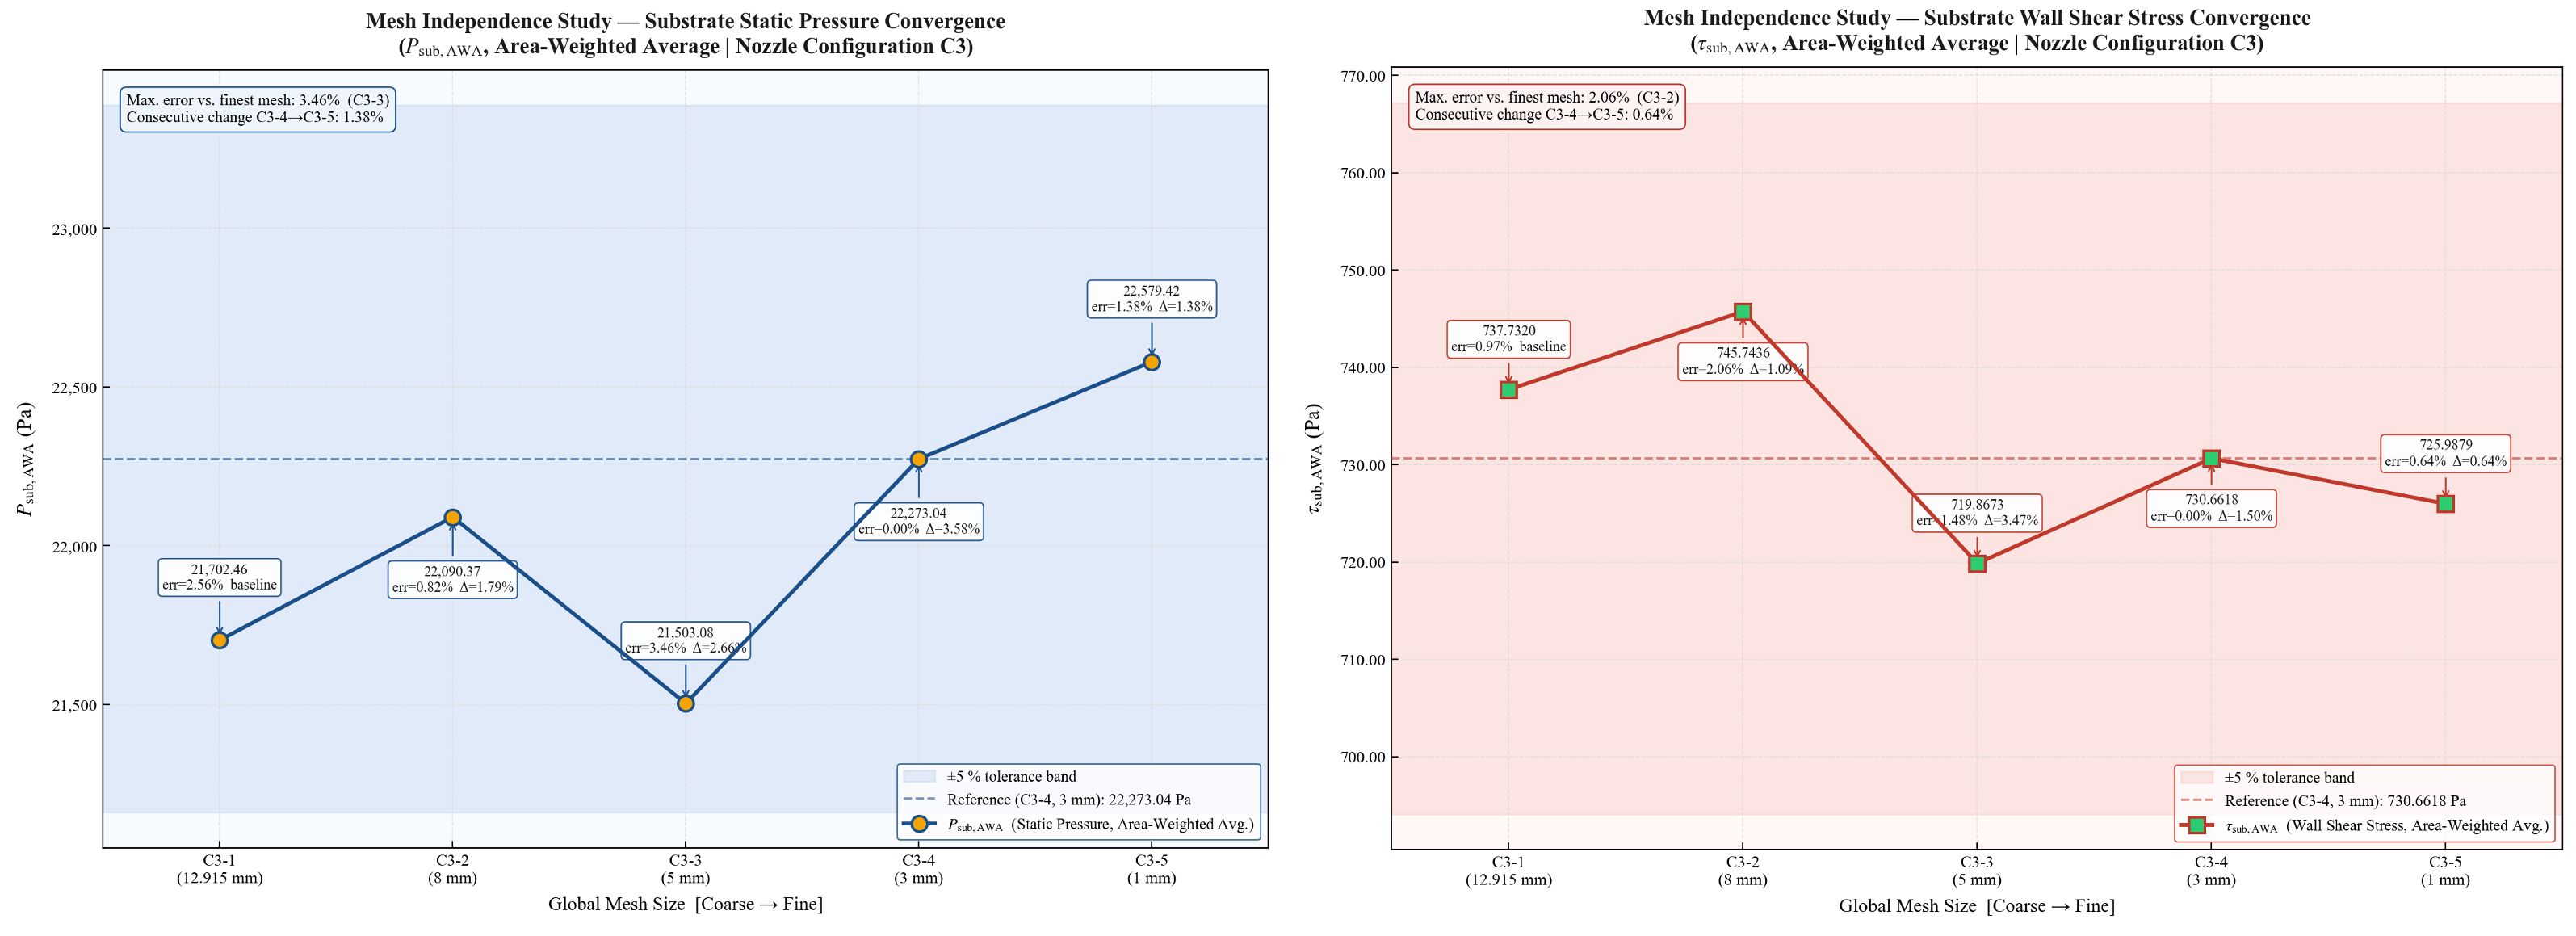
\includegraphics[width=0.9\textwidth]{figures/2.7.png}
  \caption{网格无关性验证收敛曲线（左：$P_{sub,AWA}$，右：$WSS_{nozzle}$）}
  \label{fig:2.7}
\end{figure}

以3~mm网格结果作为基准参考值，定义相对误差为：
\begin{equation}\label{eq:mesh-err}
  \varepsilon_{mesh} = \frac{|P_{sub,AWA}^{(N)} - P_{sub,AWA}^{(3mm)}|}{P_{sub,AWA}^{(3mm)}} \times 100\%.
\end{equation}
结果表明，从12.9~mm到8~mm网格，$P_{sub,AWA}$由21702~Pa降至21503~Pa，相对误差为3.5\%；从8~mm细化至5~mm时，误差降至0.8\%，已满足本研究设定的5\%收敛准则；从5~mm进一步细化至3~mm，误差仅为0.8\%，结果趋于稳定，网格无关性得到充分验证。

另外，1~mm网格虽然单元数量最多，但$P_{sub,AWA}$反而偏低（22579~Pa），且入口压力出现异常波动，偏离收敛趋势。这可能是由于在fillet曲面区域，1~mm全局网格尺寸与局部曲率不匹配，产生了高度畸变的楔形单元（最小体积达$7.9 \times 10^{-15}$~m³），诱发数值振荡。因此，1mm网格结果不纳入收敛判断。该现象同时说明：对于含曲面几何的问题，一味加密全局网格并不必然改善精度，有可能会产生截然相反的效果。针对有限元分析问题，合理的局部加密策略有时更为关键。

综合考虑计算精度与计算效率，本研究选定5~mm为推荐全局网格尺寸。在该网格方案下，$P_{sub,AWA}$与3~mm基准值的误差仅为0.8\%，远低于5\%的验收标准，同时计算时间相较3~mm方案减少约60\%，具有良好的工程实用性。本研究其余19个参数化工况均采用与C3验证工况相同的网格策略（5~mm全局尺寸、收缩段及近壁区局部加密），以确保各工况间结果的可比性。

\section{边界条件与求解设置}

\subsection{边界条件}

流体计算域入口采用速度入口边界条件，混凝土浆体速度矢量与入口截面法向一致并沿竖直向下方向施加，速度大小设定为0.03~m/s，用于表征稳定挤出工况下的进料过程；延伸段出口采用压力出口边界条件，静压设为0~Pa（表压），以模拟外界大气环境并减弱出口回压对内部流场的影响；其余所有固体边界，包括喷嘴内壁、整形板壁面以及基底接触面，均统一设置为无滑移壁面条件（No-slip），壁面速度为零，用于反映混凝土浆体与固体界面间的黏附与剪切效应；同时在整个计算域中施加重力作用，方向沿Y轴负向，与前述坐标系定义一致；上述边界条件与重力设定参数统一汇总于\cref{tab:2.5}。

\begin{table}[!htb]
  \centering
  \caption{边界条件汇总}\label{tab:2.5}
  \renewcommand{\arraystretch}{1.3}
  \begin{tabular}{lllp{4.5cm}}
    \toprule
    \textbf{边界面} & \textbf{类型} & \textbf{数值设定} & \textbf{物理说明} \\
    \midrule
    velocity\_inlet   & Velocity Inlet  & $v = 0.03$ m/s        & 泵送挤出速度，法向入射 \\
    pressure\_outlet  & Pressure Outlet & 0 Pa（表压）          & 延伸段末端自由出口 \\
    wall\_nozzle      & Wall            & No-slip               & 喷嘴内壁（收缩段+直管段） \\
    wall\_trowel      & Wall            & No-slip               & 整形板各壁面（顶/侧/前） \\
    wall\_substrate   & Wall            & No-slip               & 基底面（接触压力提取面） \\
    重力              & Body Force      & $-9.81$ m/s²（Y轴）   & 开启以影响接触压力场 \\
    \bottomrule
  \end{tabular}
\end{table}

\subsection{求解器设置}

数值求解采用ANSYS Fluent压力基（Pressure-Based）稳态求解器，以适用于低速、高黏度的非牛顿流动问题。压力-速度耦合采用SIMPLE算法以保证迭代过程中的质量守恒与收敛稳定性。空间离散方面，梯度项采用Least Squares Cell Based方法进行计算，以提高非结构化网格条件下梯度重构的精度；压力项采用PRESTO!格式，以增强对低速流动及强压力梯度区域的数值稳定性；动量方程采用Second Order Upwind格式进行离散，以提高对对流项的计算精度并降低数值扩散误差。

为了在保证数值收敛的情况下提高计算效率，连续性方程残差及各速度分量残差均控制在$1 \times 10^{-4}$以下，以作为稳态收敛判定标准。在松弛因子设置上，为适应高黏度非牛顿流体的数值特性并提高计算稳定性，压力松弛因子取0.3，动量松弛因子取0.7。所有定义的求解器参数如\cref{tab:2.6}所示，基准工况的残差收敛曲线如\cref{fig:2.8}所示。

\begin{table}[!htb]
  \centering
  \caption{求解器参数设置汇总}\label{tab:2.6}
  \renewcommand{\arraystretch}{1.3}
  \begin{tabular}{llp{6cm}}
    \toprule
    \textbf{求解器选项} & \textbf{设定值} & \textbf{说明} \\
    \midrule
    求解器类型      & Pressure-Based       & 不可压缩稳态 \\
    湍流模型        & Laminar              & $Re_{general} \approx 0.007 \ll 1$ \\
    压力--速度耦合   & SIMPLE               & 收敛稳定 \\
    压力格式        & PRESTO!              & 低速高黏度推荐 \\
    动量格式        & Second Order Upwind  & 精度优先 \\
    收敛准则        & $<1 \times 10^{-4}$  & 连续性+速度分量 \\
    压力松弛因子    & 0.3                  & 高黏度保守取值 \\
    动量松弛因子    & 0.5                  & 高黏度保守取值 \\
    迭代步数        & 500（典型）          & 所有工况500步内收敛 \\
    \bottomrule
  \end{tabular}
\end{table}

\begin{figure}[!htb]
  \centering
  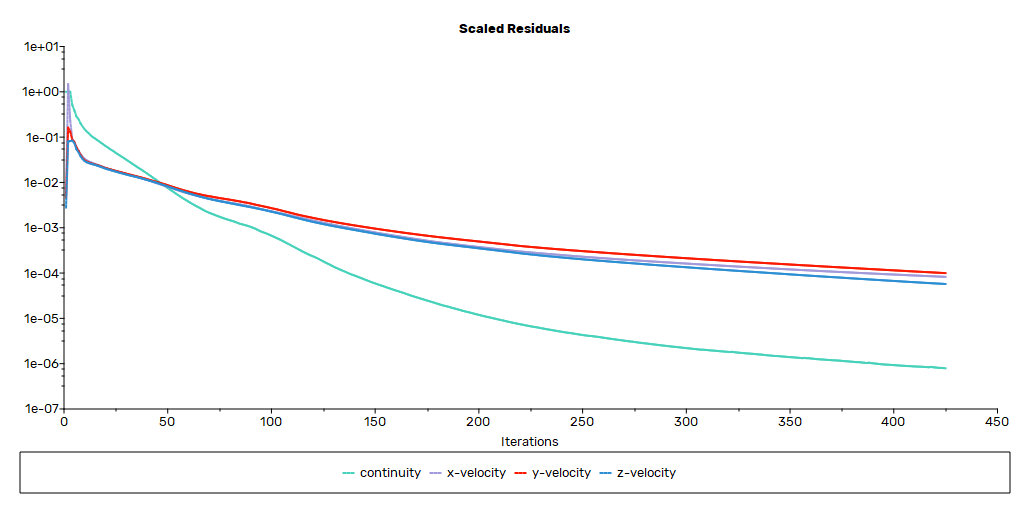
\includegraphics[width=0.8\textwidth]{figures/2.8.png}
  \caption{典型工况残差收敛曲线（Baseline工况）}
  \label{fig:2.8}
\end{figure}

\subsection{质量守恒验证}

为检验数值求解结果的稳定性与物理一致性，在ANSYS Fluent求解过程中对喷嘴入口与延伸段出口的质量流率进行监测，并记录两者差值的绝对值随迭代步数的变化曲线，用以评估质量守恒误差及收敛行为。

结果表明，所有工况在初始迭代阶段（约前50步）存在一定幅度的数值波动，随后差值逐渐衰减并趋于稳定，最终稳定在接近0的水平，说明系统在稳态求解过程中已满足质量守恒条件。由此可认为，各工况计算结果均已达到收敛状态，且数值求解具有良好的稳定性与物理合理性。基础工况的质量流率差值曲线如\cref{fig:2.9}所示。

\begin{figure}[!htb]
  \centering
  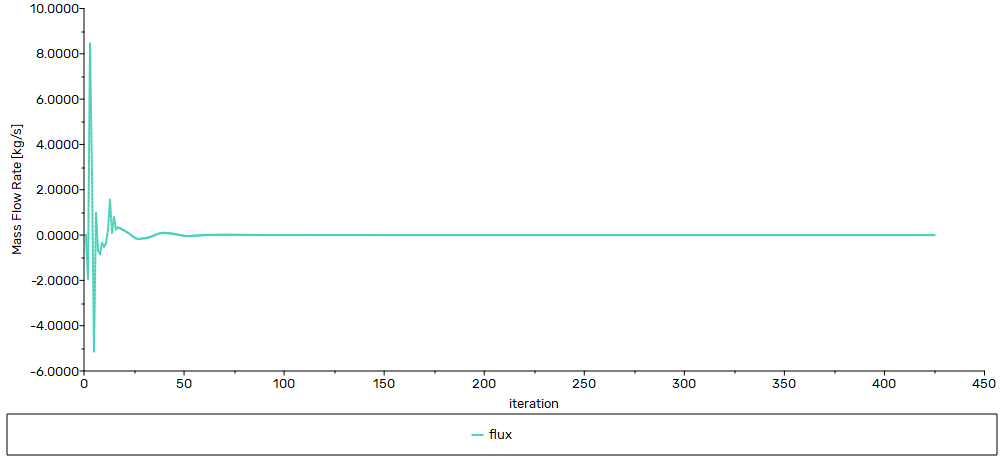
\includegraphics[width=0.8\textwidth]{figures/2.9.png}
  \caption{典型工况质量流率差值曲线（Baseline工况）}
  \label{fig:2.9}
\end{figure}

\chapter{基准工况流场分析}\label{chap:baseline}

\section{基准工况参数总结}\label{sec:baseline-params}

基线工况以He等\cite{he2024}文献报告最优工况为基础几何锚点进行建构，分别具有适中程度的喷嘴高度、喷嘴收缩角度、整形板长度以及整形板倾斜角度，具体数值总结在\cref{tab:3.1}中。其余工况在基线工况的基础上以可行域为宽度线性分布，每一组研究线包含4-5个工况，改变其中一个决定性变量进行模型重构。

\begin{table}[!htb]
  \centering
  \caption{基准工况几何参数与计算层高}\label{tab:3.1}
  \renewcommand{\arraystretch}{1.3}
  \begin{tabular}{ccccc}
    \toprule
    $\theta$ & $L$ & $TL$ & $\alpha$ & $H$ \\
    \midrule
    30° & 20 mm & 50 mm & 10° & 13.32 mm \\
    \bottomrule
  \end{tabular}
\end{table}

\section{速度场分析}

\subsection{喷嘴内速度分布与插塞流特征}

\cref{fig:3.1}展示了基准工况下喷嘴纵截面（XY平面）的速度分布云图以及入口直管段细节图。由图可见，浆体在入口直管段呈现出典型的黏塑性插塞流特征：中心区域流速均匀，截面速度梯度接近于零，对应局部剪切速率$\dot{\gamma} < \dot{\gamma}_c = 0.01~\text{s}^{-1}$，材料处于未屈服状态，形成宏观意义上的``刚性塞''；而近壁区域受固壁无滑移条件约束，速度迅速降低至零，该区域剪切速率显著高于截断值，浆体已发生屈服并产生流动。这种中心刚性、近壁流动的速度剖面是黏塑性流体在管道流动中的典型特征，与H-B流体理论预测一致。

\begin{figure}[!htb]
  \centering
  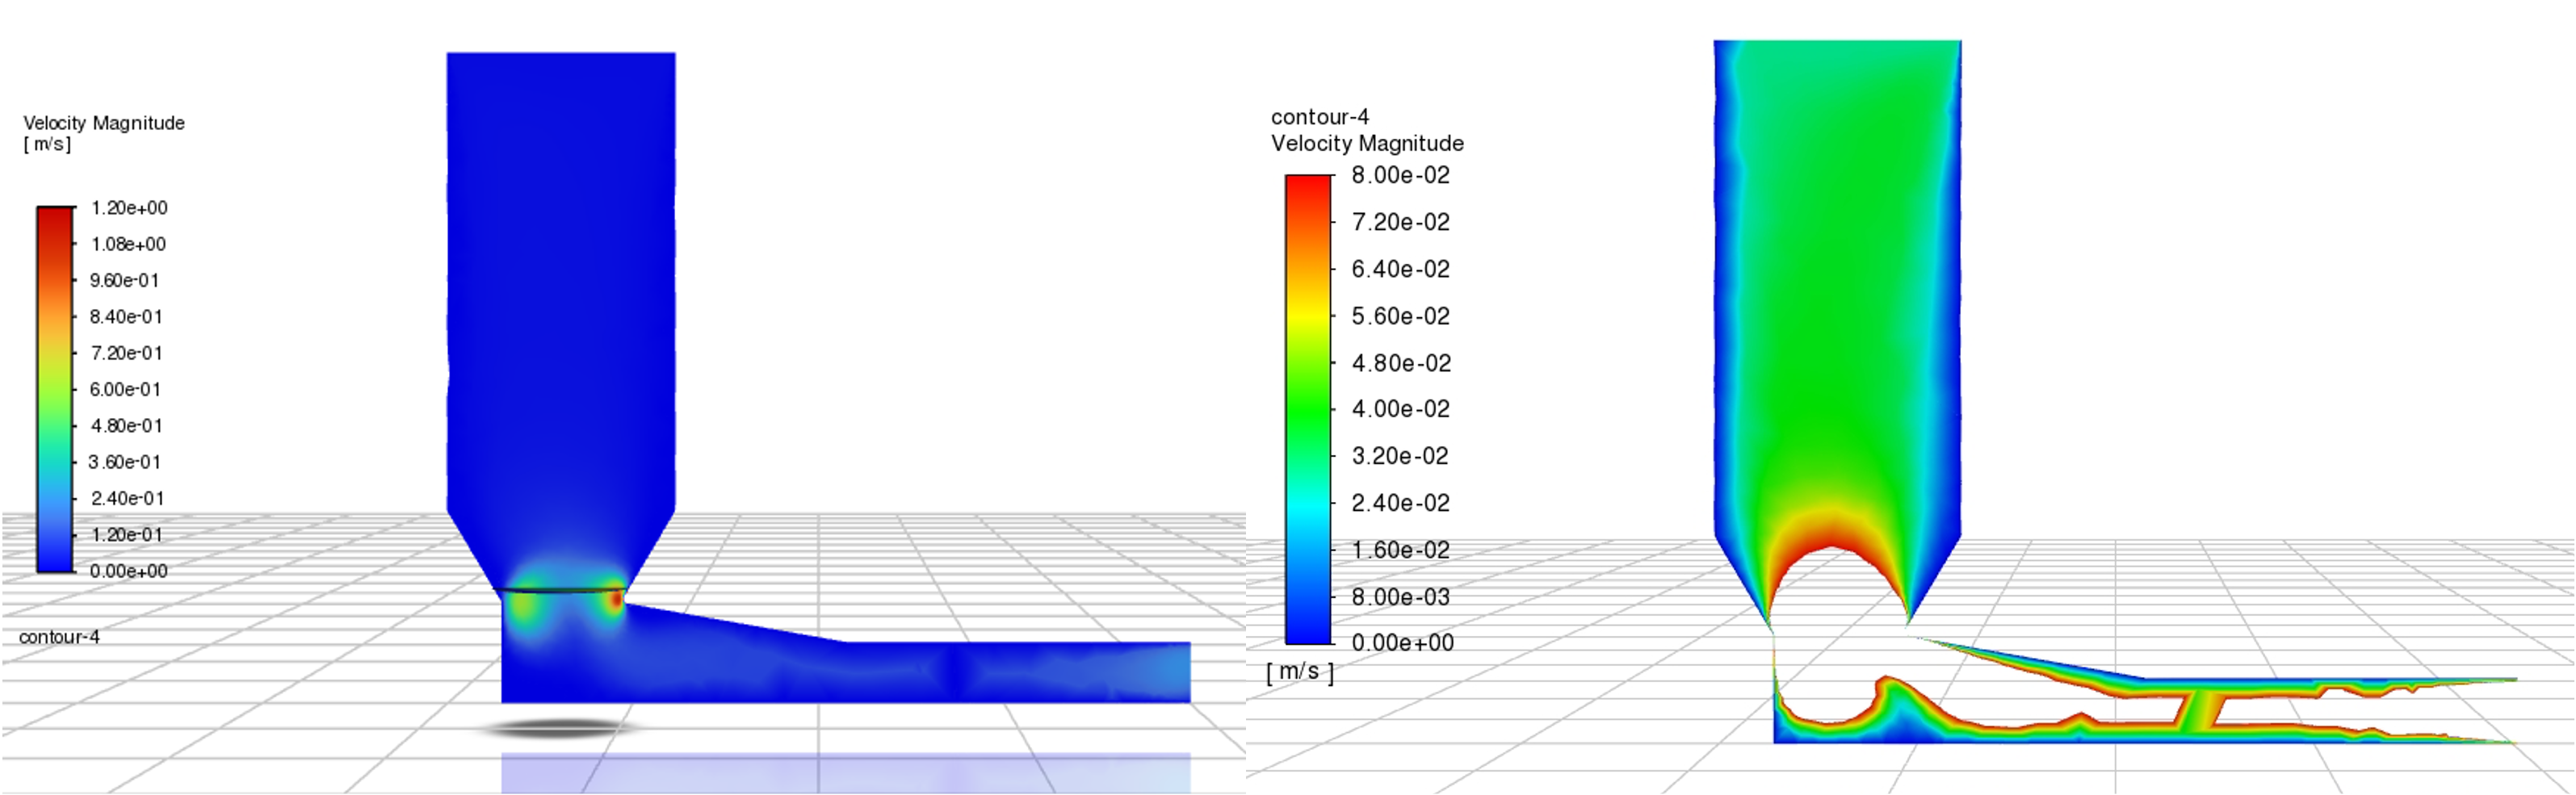
\includegraphics[width=0.85\textwidth]{figures/3.1.png}
  \caption{基准工况纵截面（XY平面）速度云图与细节图}
  \label{fig:3.1}
\end{figure}

未屈服插塞区的半径$r_{plug}$可通过壁面剪切应力$\tau_{wall}$估算。对于管道流动中的黏塑性流体，径向力平衡要求切应力沿径向线性分布，当管道中心切应力降低至等于屈服应力$\tau_0$时，即为插塞区边界，由此得到插塞区半径比的近似关系：
\begin{equation}\label{eq:rplug}
  \frac{r_{plug}}{R} = \frac{\tau_0}{\tau_{wall}},
\end{equation}
其中$R$为管道半径，$\tau_{wall}$可从CFD计算结果的喷嘴出口壁面剪切应力中提取。

基准工况下$\tau_{wall} \approx 84.93$~Pa，$\tau_0 = 500$~Pa，由\cref{eq:rplug}可得$r_{plug}/R \approx 5.9 > 1$。这说明在此工况下，喷嘴出口直管段中截断条件已基本满足，整个截面接近完全屈服状态，这与速度云图中出口截面速度分布较为均匀的观察一致。

进入收缩段后，流道截面积沿流动方向（-Y方向）单调减小，由质量守恒方程（连续性方程）可知，流速随之加速。出口截面（$D_{out} = 26$~mm）处最大流速约为1.3134~m/s，约为入口流速（0.03~m/s）的44倍，与入口截面积与出口截面积之比（$D_{in}^2 / D_{out}^2$）基本吻合，验证了质量守恒的合理性。收缩段内的强烈剪切作用使浆体屈服区域显著扩大，有利于提高挤出均匀性。收缩段喷嘴出口处的速度分布图如\cref{fig:3.2}所示。

\begin{figure}[!htb]
  \centering
  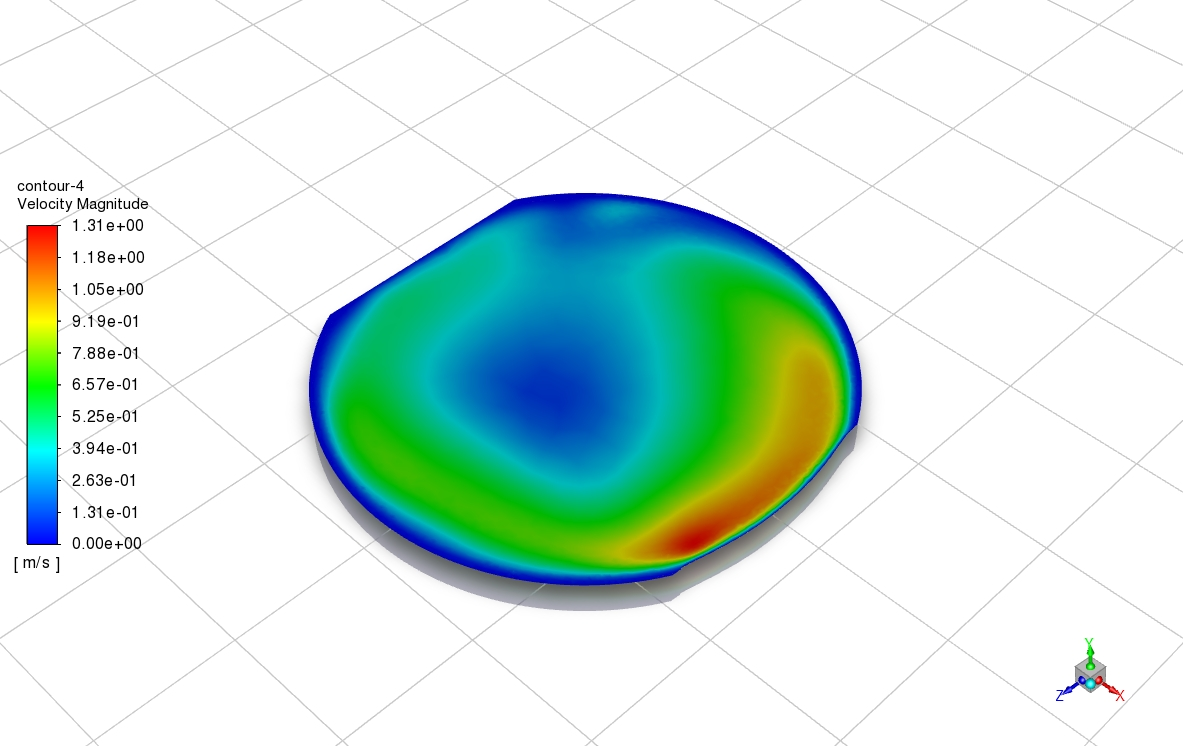
\includegraphics[width=0.7\textwidth]{figures/3.2.jpg}
  \caption{收缩段喷嘴出口处速度分布图}
  \label{fig:3.2}
\end{figure}

\subsection{整形板区域速度特征}

喷嘴的三维流线图如\cref{fig:3.3}所示。混凝土浆体离开喷嘴出口后，原本竖直向下（-Y方向）的方向在前挡板的阻挡作用下发生强制转折，转变为沿打印方向（+X方向）的横向流动。这一方向转折过程伴随着流场的剧烈重组：浆体在前挡板附近产生明显的滞止区，动压部分转化为静压，形成局部高压区。而这个局部高压区则正是基底面接触压力产生的核心驱动机制。

\begin{figure}[!htb]
  \centering
  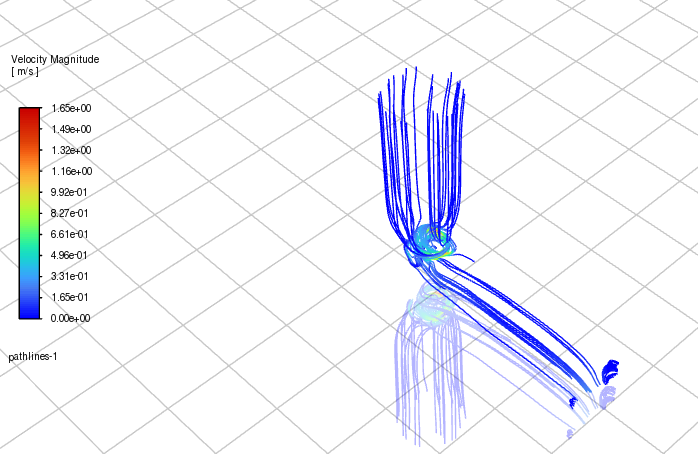
\includegraphics[width=0.75\textwidth]{figures/3.3.png}
  \caption{喷嘴三维流线图（Pathline）}
  \label{fig:3.3}
\end{figure}

在整形板受限区内，流体同时受到顶板（上方约束）、左右侧板（横向约束）和倾斜出料段（下方约束）的四面围合作用，形成封闭的楔形流动通道。受限空间内的几何约束使流体静压力得到积累，并通过倾斜出料段末端开口压向基底面，产生有效的层间接触压力。

\cref{fig:3.4}给出了整形板末端出料口的速度分布云图。由图可见，出料口截面的速度分布较为均匀，截面中心与边缘速度差较小（0.13~m/s），说明经过整形板的约束与整形作用，挤出物在离开整形板时具有较好的流动均匀性，有利于沉积层几何形态的稳定。

\begin{figure}[!htb]
  \centering
  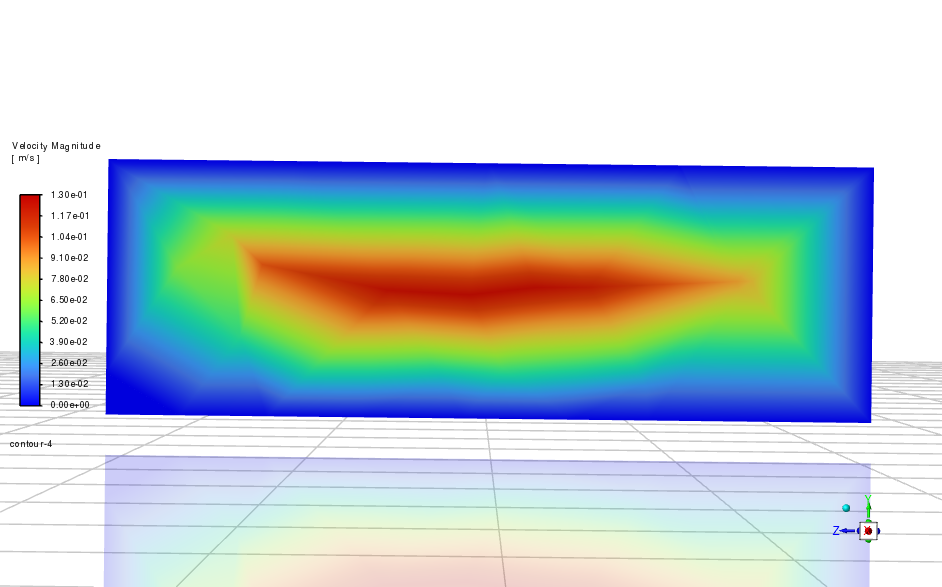
\includegraphics[width=0.7\textwidth]{figures/3.4.png}
  \caption{整形板末端出料口速度分布云图}
  \label{fig:3.4}
\end{figure}

\section{压力场分析}

\subsection{整体压力分布}

\cref{fig:3.5}与\cref{fig:3.6}分别展示了基准工况下喷嘴纵截面的压力云图与沿流动路径各监测截面的面积加权平均（Area-Weighted Average, AWA）静压力分布折线图。

\begin{figure}[!htb]
  \centering
  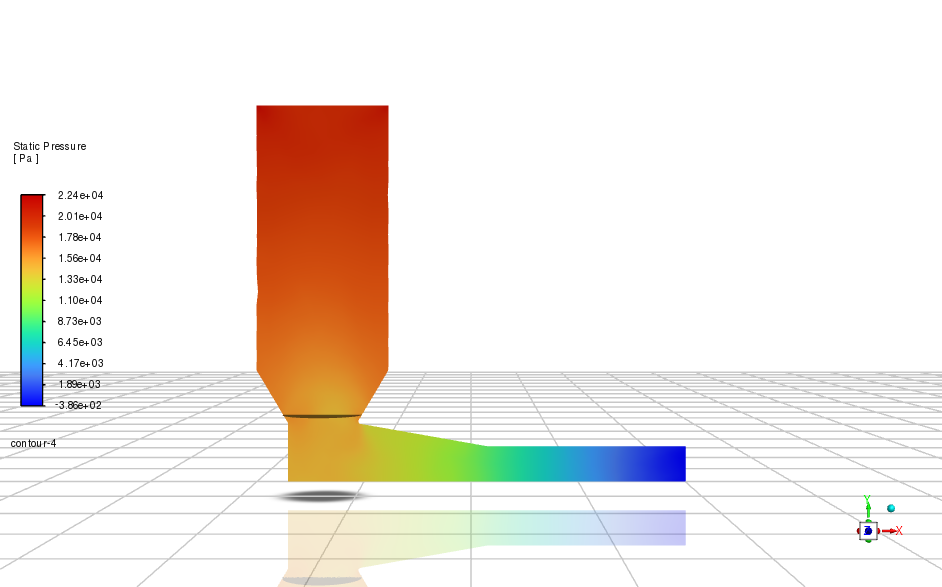
\includegraphics[width=0.7\textwidth]{figures/3.5.png}
  \caption{基准工况纵截面压力云图}
  \label{fig:3.5}
\end{figure}

\begin{figure}[!htb]
  \centering
  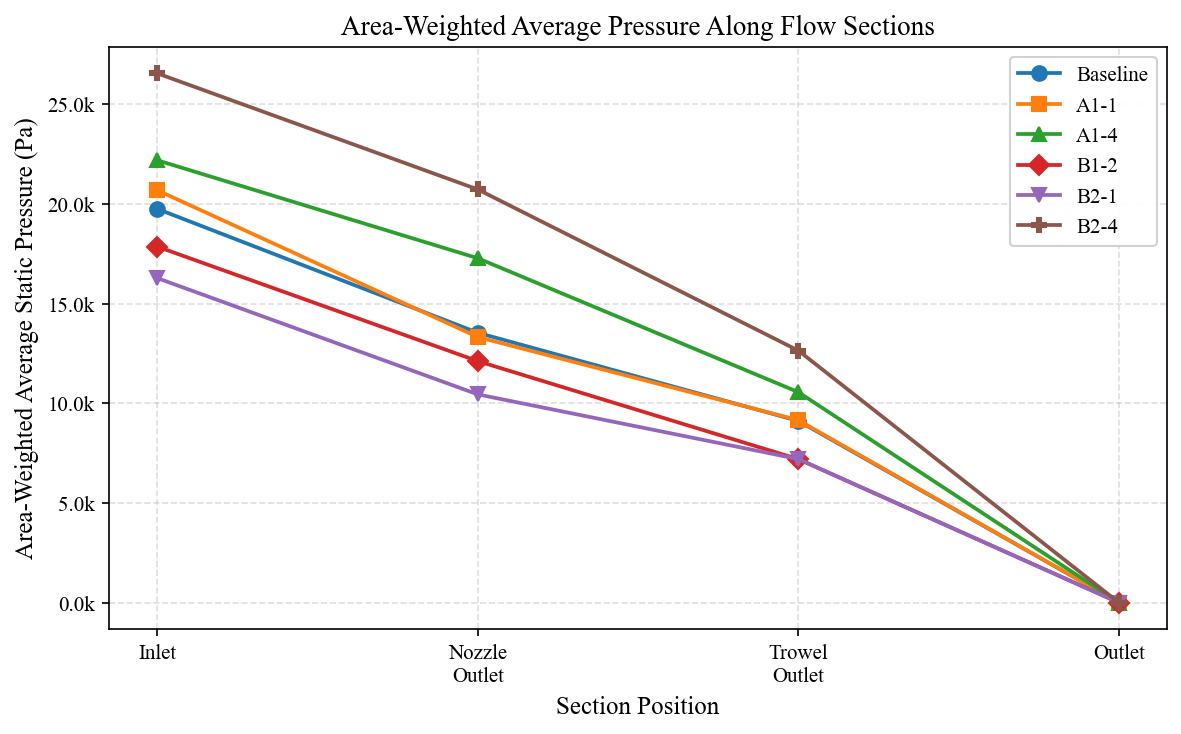
\includegraphics[width=0.8\textwidth]{figures/3.6.png}
  \caption{各截面面积加权平均压力折线图}
  \label{fig:3.6}
\end{figure}

由图可见，压力沿流动方向（从入口到出口）呈单调递减分布，这一趋势符合黏性流体流动的基本规律，驱动流体流动的压力梯度由入口泵送系统提供，并沿程克服流动阻力耗散。各截面面积加权平均压力的具体数值见\cref{tab:3.2}。

\begin{table}[!htb]
  \centering
  \caption{基准工况各截面压力汇总表}\label{tab:3.2}
  \renewcommand{\arraystretch}{1.3}
  \begin{tabular}{lccc}
    \toprule
    \textbf{截面} & \textbf{面积加权平均压力(Pa)} & \textbf{Max(Pa)} & \textbf{Min(Pa)} \\
    \midrule
    入口截面         & 19750     & 21874 & 18364 \\
    喷嘴出口截面     & 13536     & 15028 & 11830 \\
    整形板出口截面   & 9114      & 10442 & 8517 \\
    延伸段出口截面   & $\sim 0$  & 0     & -23.7 \\
    基底面           & 8310      & 13983 & -775 \\
    \bottomrule
  \end{tabular}
\end{table}

各流动区段的压降详细分析如下：

（1）收缩段压降：从喷嘴入口面（19750~Pa）至喷嘴出口面（13536~Pa），压降为5614~Pa，占总压降的约27\%。该区域压降主要由流道截面积的急剧减小引起，伴随流速大幅提升，黏性耗散显著增大。

（2）整形板受限区压降：从喷嘴出口面（13536~Pa）至整形板出口面（9114~Pa），压降为5076~Pa，约占25\%。该区段内流体受整形板四面约束，流动方向发生90°转折，局部流动阻力较大，压降集中。

（3）延伸段压降：从整形板出口面（9114~Pa）至延伸段终点（$\approx 0$~Pa），压降为9114~Pa，占46\%，是三段中最大的。模型试验中设计的75~mm延伸段并非约束区域，压力在此逐渐释放至环境压力。该区段的设置在物理上是必要的，因为如果缺少延伸段而直接在整形板末端施加出口边界条件，将导致整形板出口面处压力场失真，影响整形板约束区的计算精度，这也是本课题在几何建模时专门设置75~mm延伸段的原因。

在整形板受限区内，前挡板处动压向静压的转化是产生基底接触压力的核心机制。具体而言，浆体以较高速度（约1~m/s量级）冲击前挡板，动能转化为压力势能，在前挡板附近形成局部高压区，该高压通过流体内部压力传递作用于下方的基底面，产生层间接触压力。

\subsection{基底面压力沿打印方向分布}

基底面（Substrate，俯视XZ平面）的压力云图如\cref{fig:3.7}所示，基底面压力沿打印方向（X轴）的分布曲线如\cref{fig:3.8}所示。这两张图共同揭示了整形板约束作用下基底接触压力的空间分布特征，是本文参数化研究中各工况对比分析的基准参照。

\begin{figure}[!htb]
  \centering
  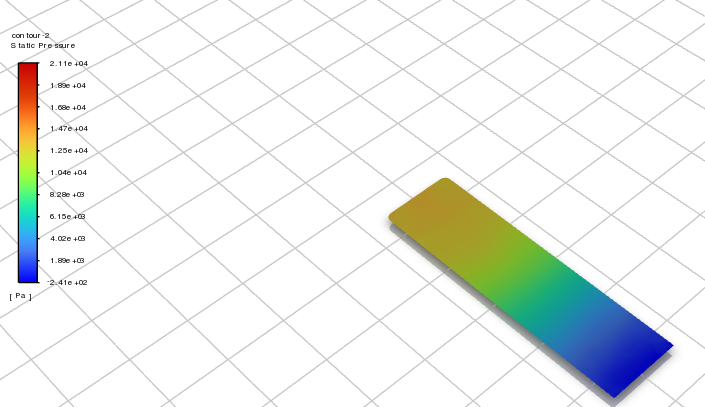
\includegraphics[width=0.75\textwidth]{figures/3.7.png}
  \caption{基底面（Substrate）压力云图（俯视，XZ平面）}
  \label{fig:3.7}
\end{figure}

\begin{figure}[!htb]
  \centering
  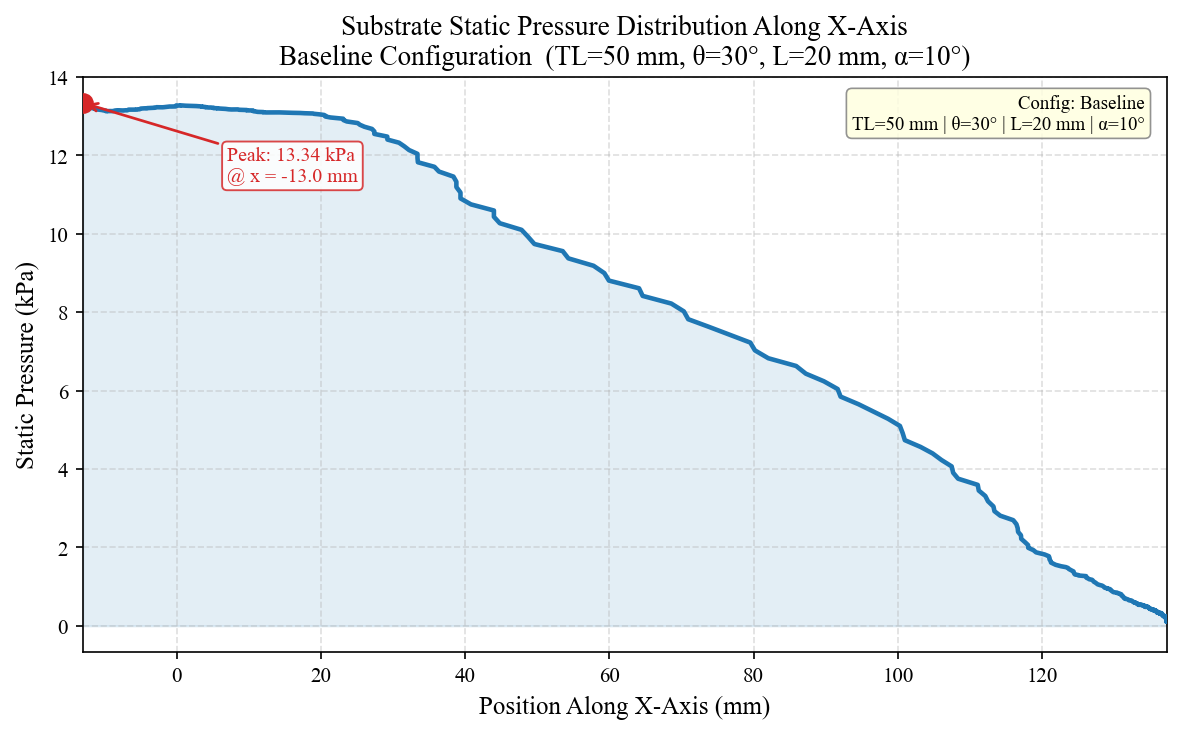
\includegraphics[width=0.8\textwidth]{figures/3.8.png}
  \caption{基底面压力沿X轴分布曲线（基准工况）}
  \label{fig:3.8}
\end{figure}

由\cref{fig:3.7}所示，基底面压力分布具有明显的空间非均匀性：高压区集中于整形板约束区域的中心偏前部，对应喷嘴出口正下方区域（$X \approx 0$附近），面积加权平均压力达到8310~Pa，最大压力峰值为13983~Pa。

\cref{fig:3.8}的XY曲线提供了更清晰的沿程分布信息。压力从整形板入口端（$X \approx 0$）的峰值13983~Pa开始，沿打印方向（+X方向）随着流体远离高压约束区而逐渐衰减，在延伸段末端附近，压力降至接近零甚至出现轻微负值（$-775$~Pa）。基底面压力在前26~mm出现了一个平台期，而这部分区域也正是喷嘴出料口面的宽度；随后，沿程压力得到了逐步释放。

基底面压力负压区的出现具有明确的物理成因：浆体流经整形板末端时，受约束突然释放，流体在出料口后缘发生局部流动分离，导致局部压力低于环境压力。负压区的量值较小（$<1$~kPa），对整体接触压力的评估影响有限，但其存在说明整形板末端的几何形状（倾斜角$\alpha$）对该区域的压力分布有显著影响，将在\cref{chap:parametric}第\ref{sec:alpha-influence}节的参数化分析中进一步讨论。

\section{剪切应力与黏度分布}

\subsection{剪切速率分布与插塞流区域}

\cref{fig:3.9}给出了基准工况下喷嘴纵截面的剪切速率分布云图。

\begin{figure}[!htb]
  \centering
  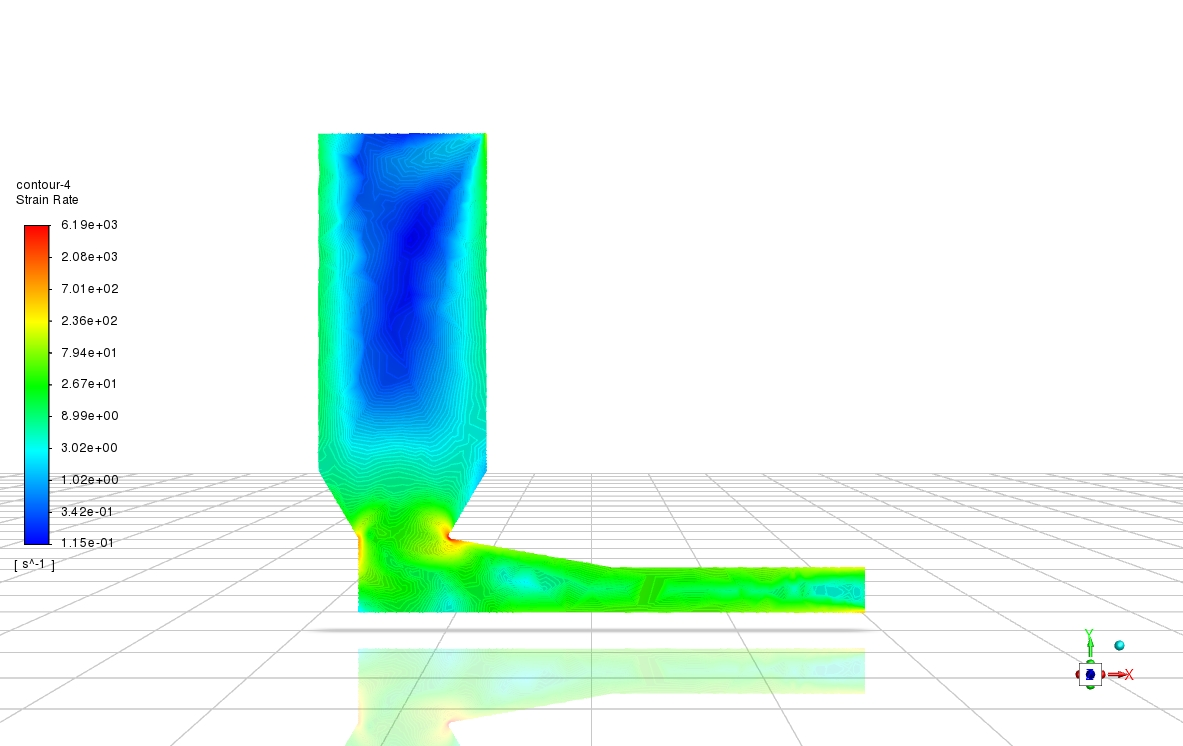
\includegraphics[width=0.7\textwidth]{figures/3.9.jpg}
  \caption{剪切速率分布云图（纵截面）}
  \label{fig:3.9}
\end{figure}

在CFD计算中，局部剪切速率$\dot{\gamma}$由应变速率张量$\mathbf{D}$的二阶不变量定义：
\begin{equation}\label{eq:shear-rate}
  \dot{\gamma} = \sqrt{2 \mathbf{D} : \mathbf{D}},
\end{equation}
\begin{equation}\label{eq:strain-rate}
  \mathbf{D} = \frac{1}{2} (\nabla \mathbf{u} + \nabla \mathbf{u}^T).
\end{equation}
由\cref{fig:3.9}可见，剪切速率的空间分布高度不均匀，呈现出显著的分区特征：

高剪切速率区（$\dot{\gamma} \gg \dot{\gamma}_c$）主要集中于两个位置：（1）喷嘴收缩段的近壁区域：喷嘴收缩段壁面急剧收缩，近壁区域的速度梯度最大，最大剪切速率达到6190~s⁻¹；（2）整形板受限区与前挡板附近：流体在此处经历强制方向转折，局部速度梯度同样较大。

低剪切速率区（$\dot{\gamma} < \dot{\gamma}_c$，未屈服plug zone）则占据入口直管段的中心区域，以及整形板受限区中流速较为均匀的区段。

这种剪切速率的分区分布对打印质量具有双重意义：一方面，高剪切区内浆体已充分屈服，流动阻力较低，有利于挤出顺畅；另一方面，过高的剪切速率会导致浆体结构破坏，可能降低早龄期强度，不利于沉积后的形状保持。因此，合理控制喷嘴内的剪切速率分布是喷嘴设计优化的重要目标之一。

\subsection{黏度场与屈服区}

黏度场分布云图如\cref{fig:3.10}所示。

\begin{figure}[!htb]
  \centering
  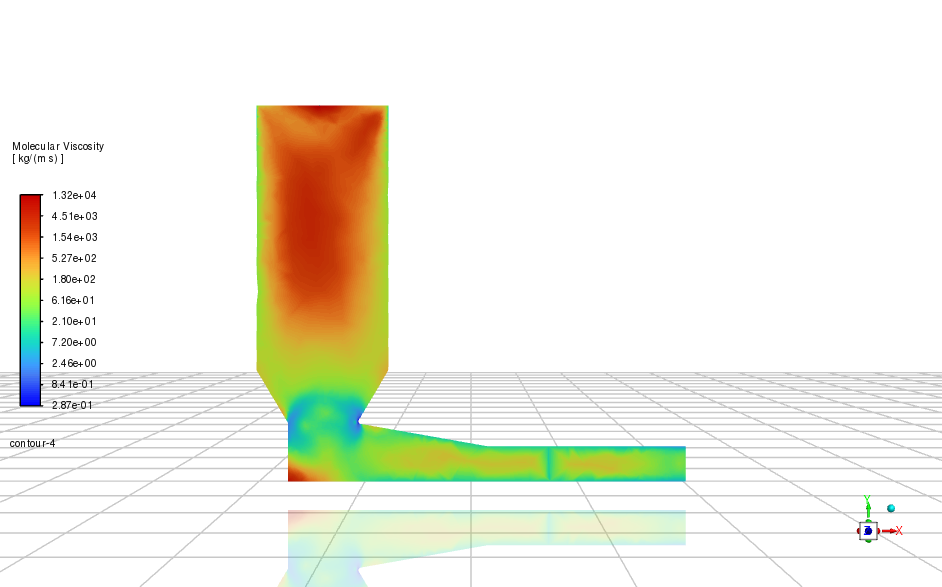
\includegraphics[width=0.7\textwidth]{figures/3.10.png}
  \caption{黏度分布云图（纵截面）}
  \label{fig:3.10}
\end{figure}

由H-B本构模型可知，表观黏度$\eta$与剪切速率$\dot{\gamma}$存在一一对应关系：剪切速率越高，表观黏度越低（剪切变稀）；在未屈服区（$\dot{\gamma} \leq \dot{\gamma}_c$），黏度取截断上限值为$\eta_{max} = 50000$~Pa·s，近似模拟固体行为。

由图可见，黏度场与剪切速率场呈镜像对应关系：喷嘴中心未屈服区黏度接近$\eta_{max}$（图中深色区域），而收缩段近壁高剪切区黏度降低3-4个数量级，最低可至$\eta_{min} = 1$~Pa·s附近（图中浅色区域）。这一量级的黏度差异（约$10^4$倍）是非牛顿流体CFD模型的典型特征，也验证了H-B模型的Papanastasiou正则化处理在本工况下使用的合理性。

\cref{fig:3.11}进一步通过布尔提取的方式，直观展示了屈服区（$\dot{\gamma} > \dot{\gamma}_c$，图中红色）与未屈服区（$\dot{\gamma} \leq \dot{\gamma}_c$，图中蓝色）的空间边界。从层间粘结的角度来看，已屈服的浆体具有一定的流动性，沉积时有利于与前一层浆体发生界面融合，提升层间粘结强度；而大量未屈服材料的存在则有利于沉积后的形状保持，防止层体在自重作用下坍塌。因此，屈服区与未屈服区的合理分布对于3D打印质量具有重要意义，喷嘴几何参数（尤其是收缩角$\theta$）对这一分布的影响将在\cref{chap:parametric}中进一步量化分析。

\begin{figure}[!htb]
  \centering
  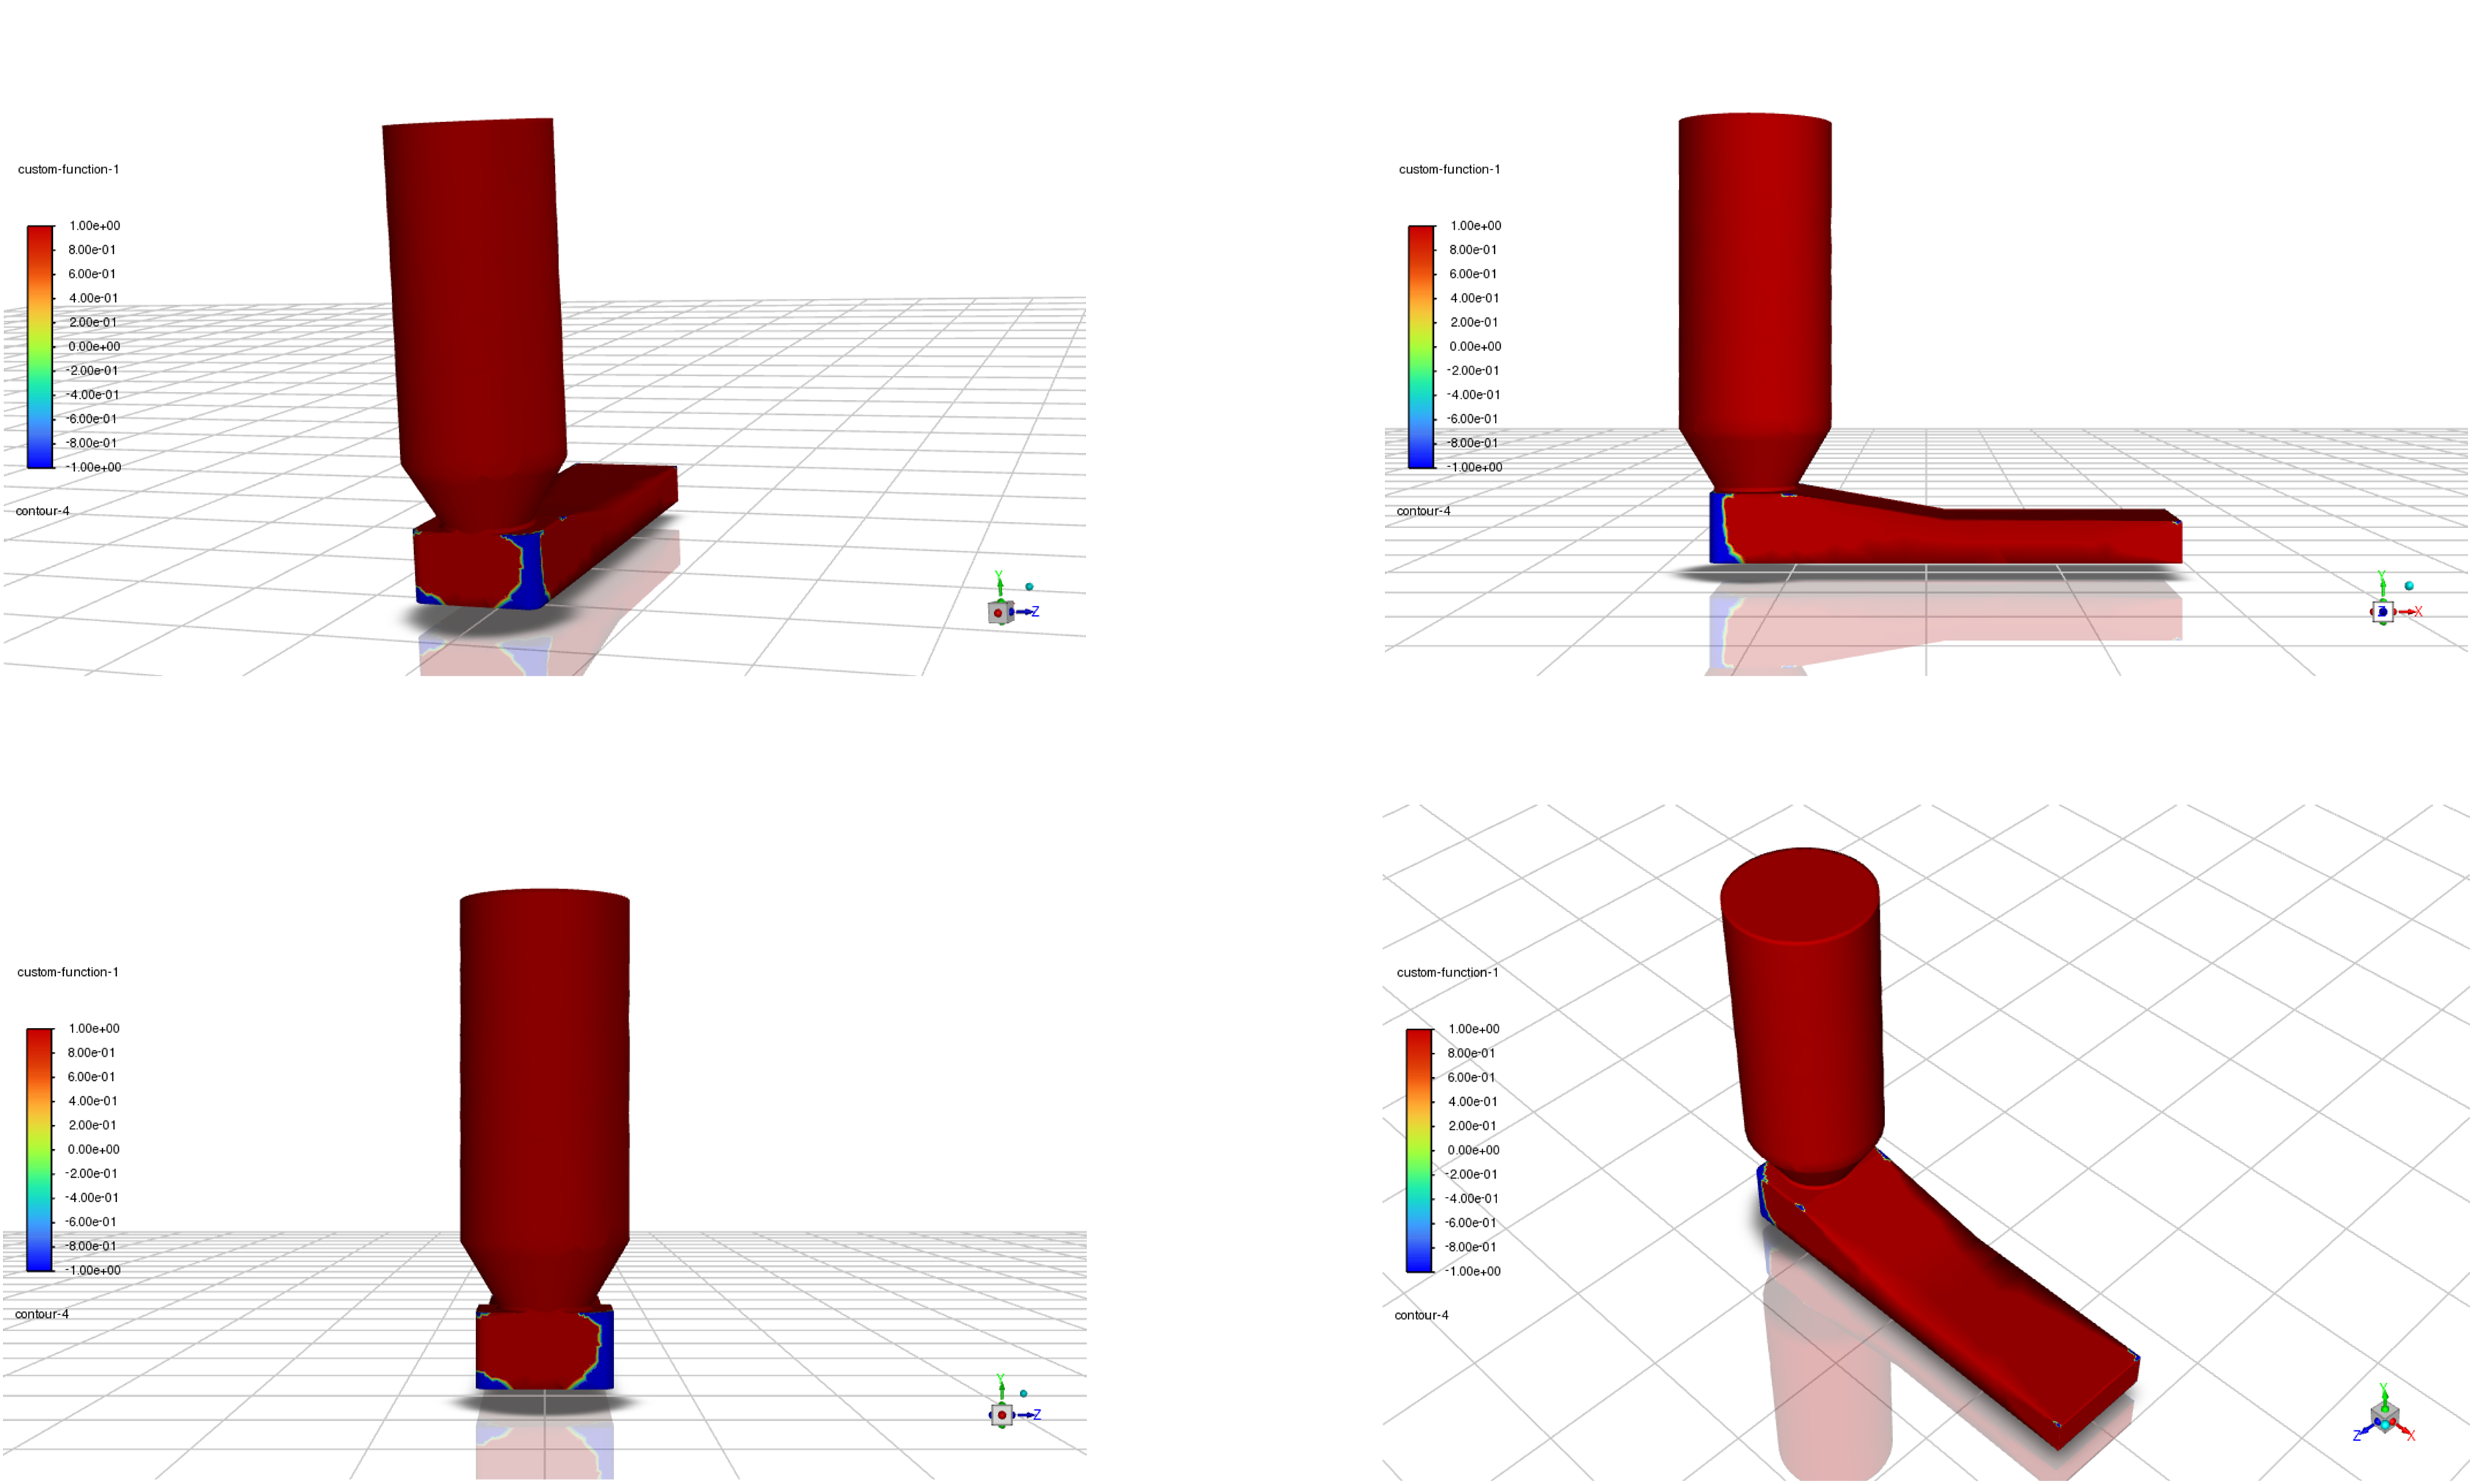
\includegraphics[width=0.7\textwidth]{figures/3.11.png}
  \caption{屈服区/未屈服区分布示意图（布尔提取）}
  \label{fig:3.11}
\end{figure}

\subsection{壁面剪切应力}

壁面的壁面剪切应力（Wall Shear Stress, WSS）分布云图如\cref{fig:3.12}所示。壁面剪切应力反映了浆体在壁面附近的黏性阻力强度，是喷嘴磨损寿命预测和材料剪切损伤评估的重要参数。

\begin{figure}[!htb]
  \centering
  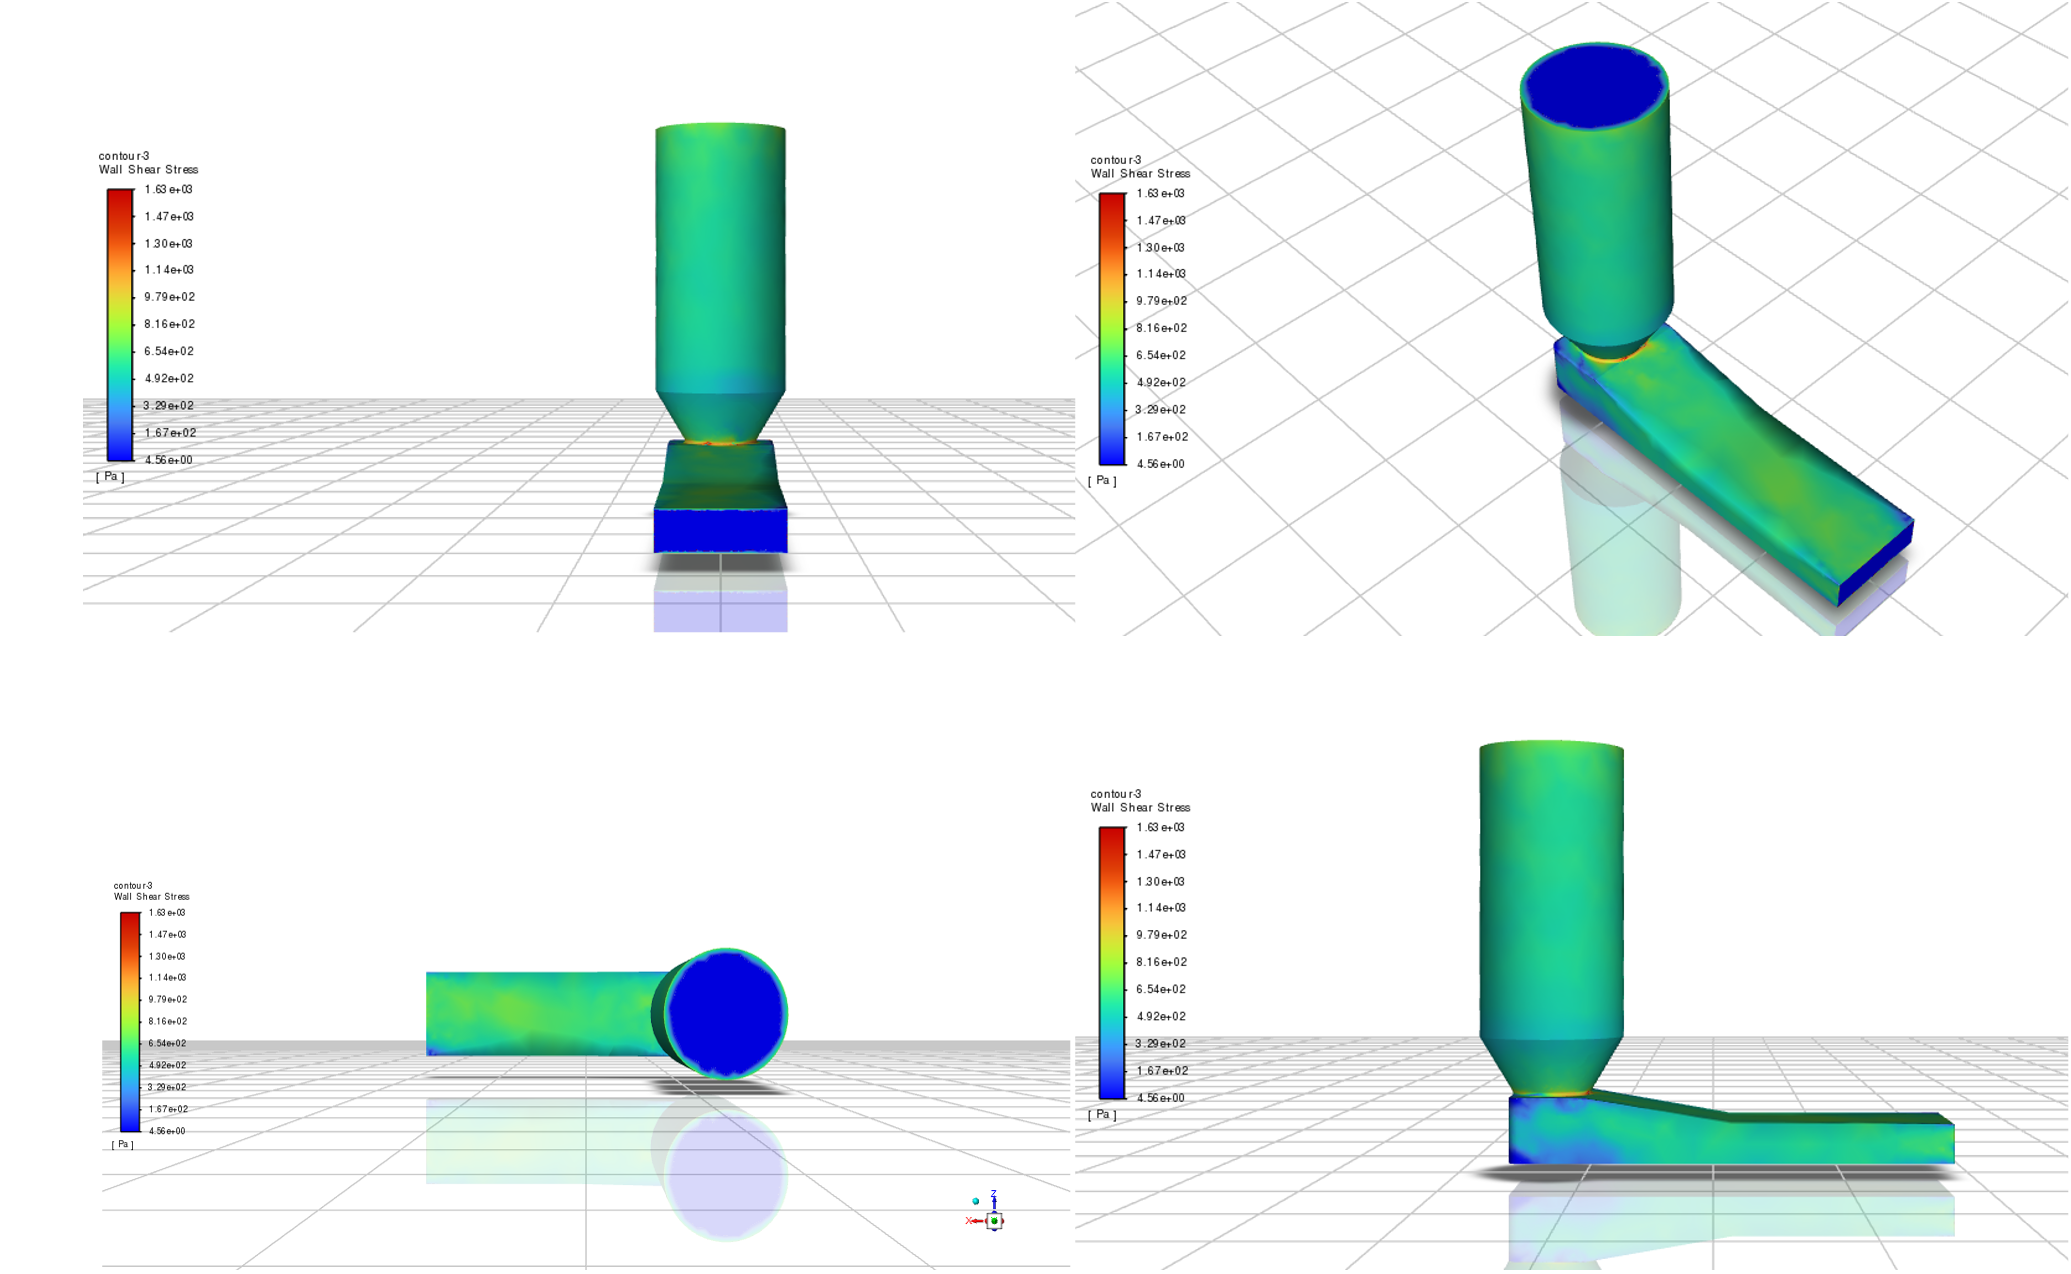
\includegraphics[width=0.75\textwidth]{figures/3.12.png}
  \caption{壁面剪切应力分布云图}
  \label{fig:3.12}
\end{figure}

由\cref{fig:3.12}及\cref{tab:3.2}中的定量数据可知，各壁面的壁面剪切应力分布存在显著差异。喷嘴出口截面的面积加权平均壁面剪切应力为84.9~Pa，反映了喷嘴内壁在出口段承受的平均剪切载荷；整形板末端出料口的面积加权平均壁面剪切应力则为172.7~Pa，高于喷嘴出口，这是因为整形板末端流道截面积较小（受倾斜角$\alpha$约束），流速梯度更大，壁面剪切载荷相应增大。从喷嘴设计的工程角度来看，壁面剪切应力越大，喷嘴固件的磨损就越快、材料就会越容易受到剪切破坏。因此，在追求高接触压力的同时，还需兼顾对壁面剪切应力的控制。

基底面的壁面剪切应力则反映了浆体对已打印层基底面的切向作用力。该值过大可能导致基底表面材料被撕裂或已打印层结构被破坏，是评估打印工艺对已沉积层影响的重要指标。

\chapter{参数化研究}\label{chap:parametric}

\section{参数化研究设计框架}

\subsection{设计变量与工况矩阵}

依照单因素变化原则，本课题共设计三组别20个喷嘴工况，分别调整喷嘴收缩角$\theta$、喷嘴竖向长度$L$、整形板倾斜角$\alpha$以及整形板延伸长度$TL$四个控制变量，分别设计4-5组不同工况，研究喷嘴参数（A组）、整形板参数（B组）对混凝土喷嘴挤出机制的影响，并同时设计对照优化组（C组），探索四控制变量下的最优解。

定义工况的几何参数矩阵如\cref{tab:4.1}所示。

\begin{table}[!htb]
  \centering
  \caption{工况完整参数矩阵与 $P_{sub,AWA}$ 结果}\label{tab:4.1}
  \renewcommand{\arraystretch}{1.2}
  \footnotesize
  \begin{tabular}{lccccccp{3cm}}
    \toprule
    \textbf{工况} & $TL$ & $\theta$ & $L$ & $\alpha$ & $H$ (mm) & $P_{sub,AWA}$ (Pa) & \textbf{组别说明} \\
    \midrule
    Baseline & 50 & 30° & 20 & 10° & 13.32 & 8310  & 基准工况 \\
    A1-1     & 50 & 15° & 20 & 10° & 13.32 & 8286  & 研究线A1：$\theta$变化 \\
    A1-2     & 50 & 0°  & 20 & 10° & 13.32 & 8357  &  \\
    A1-3     & 50 & 45° & 20 & 10° & 13.32 & 9130  &  \\
    A1-4     & 50 & 60° & 20 & 10° & 13.32 & 9926  &  \\
    A2-1     & 50 & 30° & 10 & 10° & 13.32 & 8323  & 研究线A2：$L$变化 \\
    A2-2     & 50 & 30° & 30 & 10° & 13.32 & 8905  &  \\
    A2-3     & 50 & 30° & 40 & 10° & 13.32 & 9382  &  \\
    B1-1     & 50 & 30° & 20 & 0°  & 22.00 & 5733  & 研究线B1：$\alpha$变化 \\
    B1-2     & 50 & 30° & 20 & 5°  & 17.64 & 6896  &  \\
    B1-3     & 50 & 30° & 20 & 15° & 9.06  & 12081 &  \\
    B1-4     & 50 & 30° & 20 & 20° & 4.90  & 22184 &  \\
    B2-1     & 30 & 30° & 20 & 10° & 16.79 & 5944  & 研究线B2：$TL$变化 \\
    B2-2     & 40 & 30° & 20 & 10° & 15.05 & 7177  &  \\
    B2-3     & 60 & 30° & 20 & 10° & 11.58 & 10353 &  \\
    B2-4     & 70 & 30° & 20 & 10° & 9.85  & 12833 &  \\
    C1-1     & 50 & 60° & 20 & 10° & 13.32 & 9926  & C组：A组最优 \\
    C1-2     & 55 & 30° & 20 & 15° & 7.77  & 14525 & C组：Trowel优化 \\
    C1-3     & 60 & 60° & 20 & 15° & 6.47  & 21677 & C组：性能最优 \\
    C2       & 0  & 30° & 20 & 10° & 22.00 & 3436  & C组：无顶板对照组 \\
    C3       & 60 & 60° & 20 & 15° & 6.47  & 21702 & C组：含Fillet几何优化 \\
    \bottomrule
  \end{tabular}
\end{table}

\subsection{评价指标定义}

喷嘴的性能评价是一个复杂的多目标体系，其几何特征会直接影响能效传递、层间粘结性能、材料损伤风险、泵送经济性、压力均匀性等等方面，而在实际工程实践当中，往往需要对这些指标进行综合评判，找到一个性能最优的解决方案。本课题定义了五项评价指标，从多个角度对喷嘴工况的表现进行量化与评价。

（1）基底面积加权平均压力$P_{sub,AWA}$：基底面积加权平均压力$P_{sub,AWA}$是本课题最核心的评价指标之一，定义为打印基底面上各网格单元静压力以面积为权重的加权平均值。这项指标是整形板对浆体施加的平均接触压力的反映，可以间接反映层间粘结强度。较高的接触压力有助于压实层间界面，促进水泥浆料的界面融合，提升层间抗剪和抗拉强度。

（2）喷嘴出口截面壁面剪切应力$WSS_{nozzle}$：喷嘴出口截面壁面剪切应力$WSS_{nozzle}$是喷嘴出口处壁面剪切应力的面积加权平均值。这个指标反映了喷嘴内壁在出口区域所承受的切向摩擦载荷，与喷嘴磨损速率正相关；于此同时，过高的剪切应力可能导致打印混凝土浆体的结构网络被过度破坏，影响挤出后的形状保持能力与早龄期强度发展。

（3）压力传递效率$\eta_p$：压力传递效率$\eta_p$是基底面面积加权平均压力与入口面积加权平均压力之比，公式表达为：
\begin{equation}\label{eq:eta-p}
  \eta_p = \frac{P_{sub,AWA}}{P_{inlet,AWA}}.
\end{equation}
该指标反映了泵送系统施加的驱动压力中，最终转化为基底有效接触压力的比例，是衡量打印系统压力利用经济性的无量纲指标。$\eta_p$越大，说明系统在相同泵送能耗下能够产生更高的层间接触压力，系统整体效率越高。

（4）压力非均匀性指数$UI$（Uniformity Index）：压力非均匀性指数$UI$是基底面压力最大值与最小值之差相对于面积加权平均压力的比值，公式表达为：
\begin{equation}\label{eq:UI}
  UI = \frac{P_{sub,Max} - P_{sub,Min}}{P_{sub,AWA}}.
\end{equation}
压力非均匀性指数反映了基底面接触压力的空间分布均匀程度。$UI$越小，整形板对基底面的压力分布越均匀，有利于层间粘结质量的空间一致性；$UI$过大，意味着局部压力集中，可能导致层间粘结强度的空间不均匀。

（5）入口面积加权平均压力$P_{inlet}$：$P_{inlet}$作为泵送能耗的代理指标，反映了打印系统维持稳定挤出所需的泵送驱动压力。$P_{inlet}$越小，对泵送设备的压力要求越低，打印系统的能耗与设备成本越低。

\section{喷嘴收缩角$\theta$的影响（A1组工况）}

为研究喷嘴收缩角度对喷嘴挤出性能的影响，本课题共选取5组工况进行了参数化研究。\cref{tab:4.2}总结了5组工况重点研究指标的结果。

\begin{table}[!htb]
  \centering
  \caption{A1组（$\theta$变化）各工况评价指标汇总表}\label{tab:4.2}
  \renewcommand{\arraystretch}{1.3}
  \begin{tabular}{lccccccl}
    \toprule
    \textbf{工况} & $\theta$ & $P_{sub}$(Pa) & $WSS_{nozzle}$ & $\eta_p$ & $UI$ & $P_{inlet}$ & \textbf{综合} \\
    \midrule
    A1-1     & 15° & 8286  & 96.9 & 0.401 & 1.73 & 20685 & \\
    A1-2     & 0°  & 8357  & 89.3 & 0.370 & 1.75 & 22584 & \\
    Baseline & 30° & 8310  & 84.9 & 0.421 & 1.78 & 19750 & \\
    A1-3     & 45° & 9130  & 64.4 & 0.426 & 1.76 & 21451 & \\
    A1-4     & 60° & 9926  & 35.0 & 0.447 & 1.84 & 22190 & 最优 \\
    \bottomrule
  \end{tabular}
\end{table}

\subsection{$\theta$对基底压力的影响}

五种收缩角工况下的压力云图如\cref{fig:4.1}所示，$P_{sub,AWA}$随收缩角$\theta$变化的折线图如\cref{fig:4.2}所示。

\begin{figure}[!htb]
  \centering
  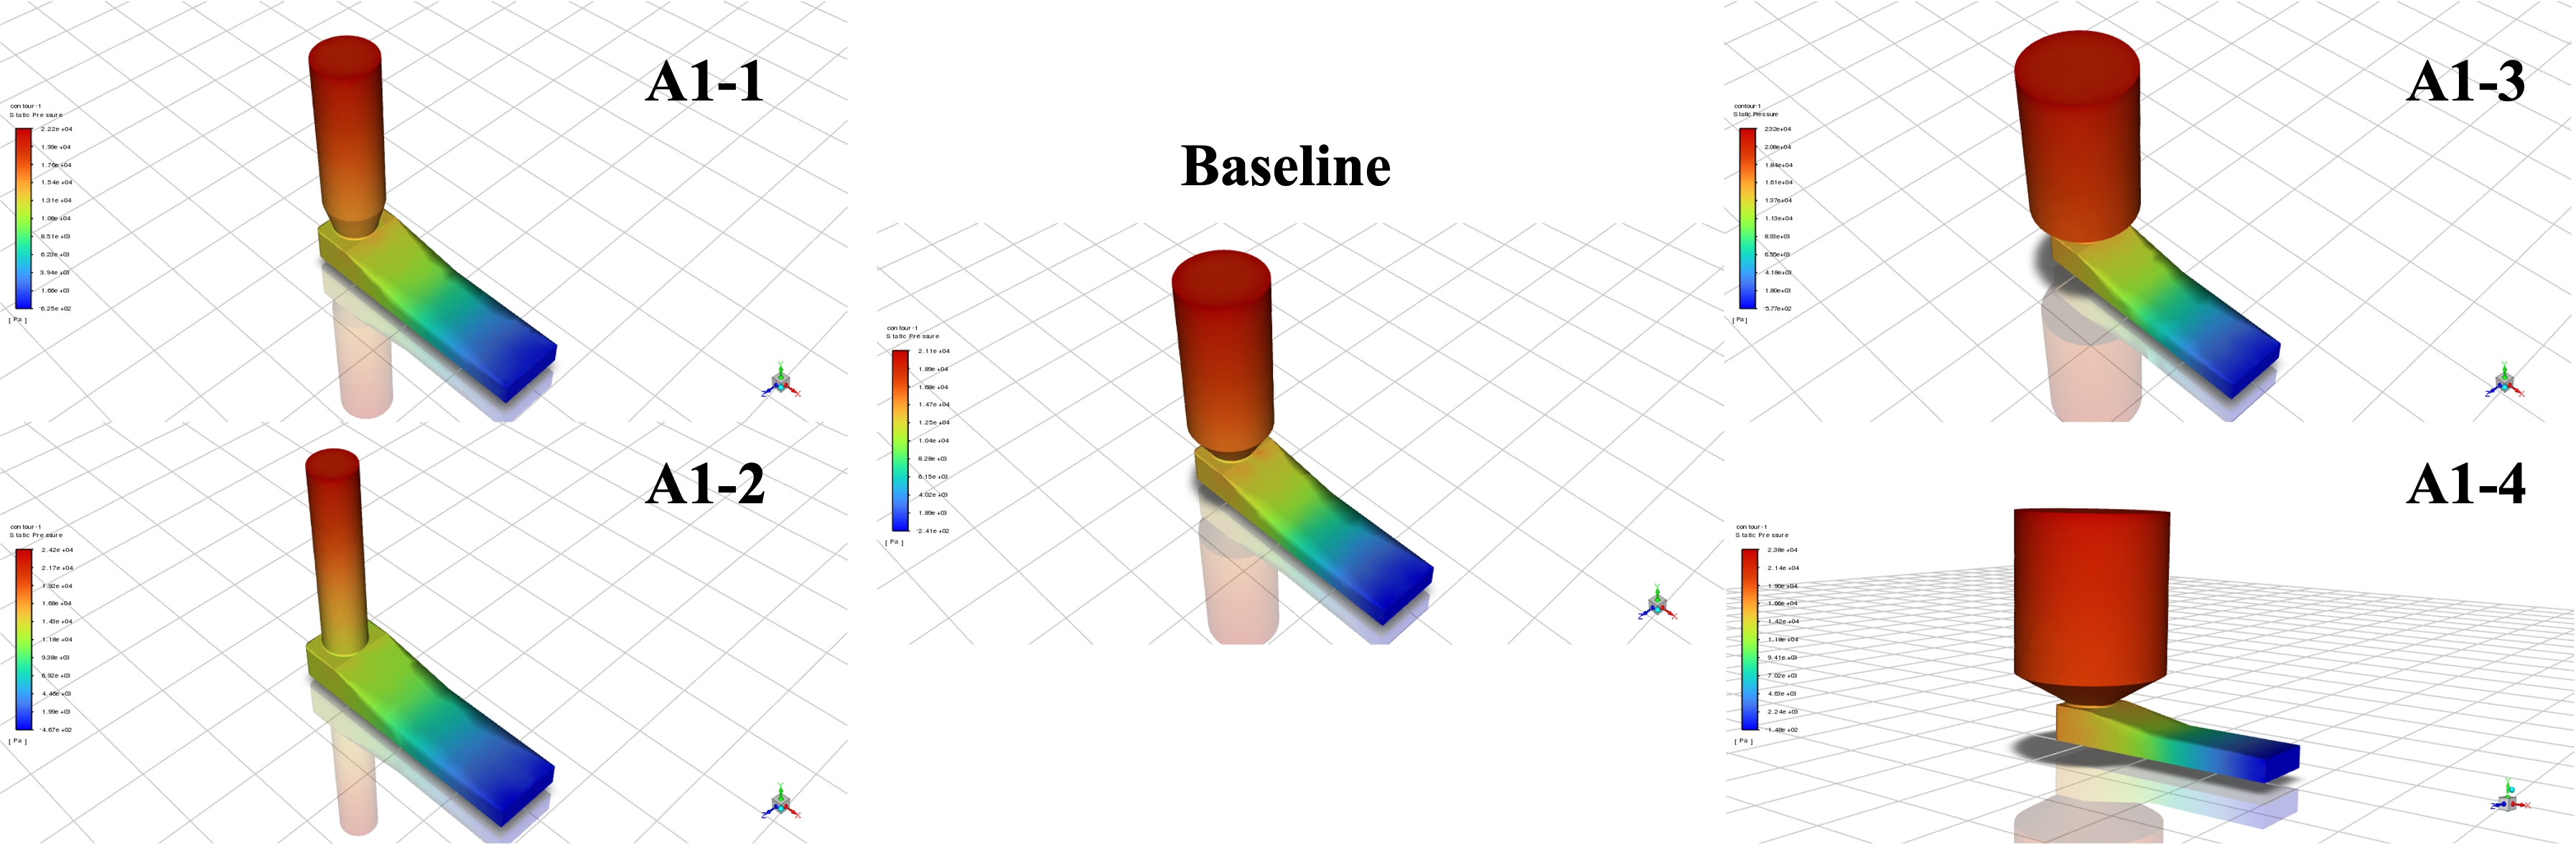
\includegraphics[width=0.9\textwidth]{figures/4.1.png}
  \caption{不同$\theta$下纵截面压力云图对比图}
  \label{fig:4.1}
\end{figure}

\begin{figure}[!htb]
  \centering
  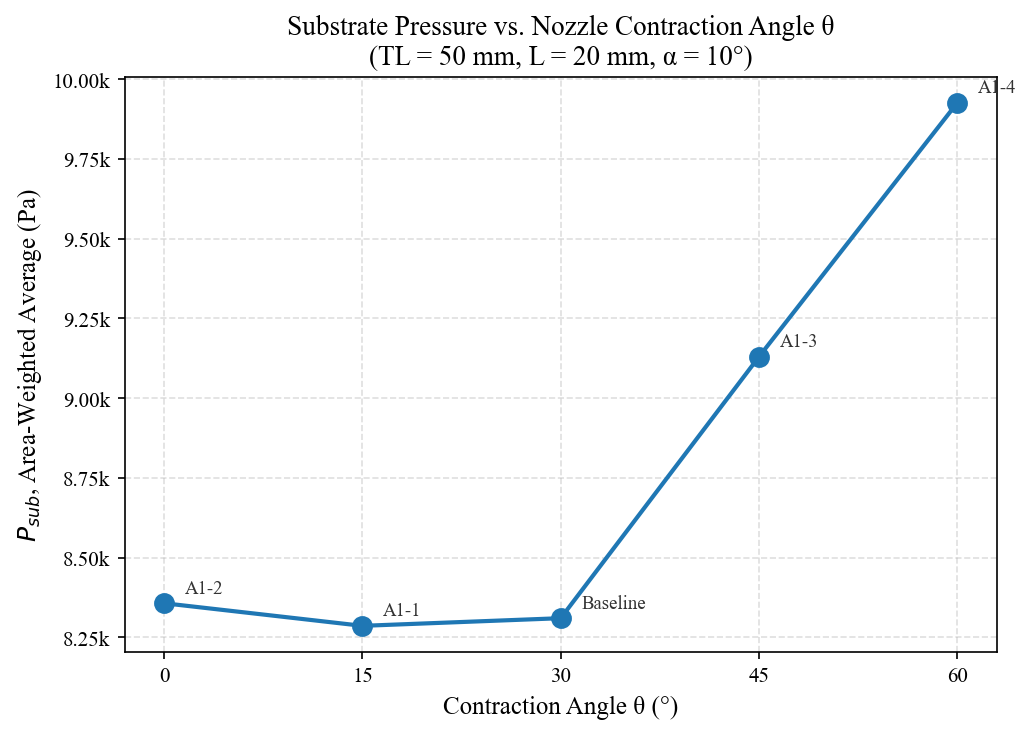
\includegraphics[width=0.75\textwidth]{figures/4.2.png}
  \caption{$P_{sub,AWA}$--$\theta$变化折线图}
  \label{fig:4.2}
\end{figure}

由图可见，随着收缩角$\theta$从0°增大至60°，$P_{sub,AWA}$大致呈平坦-递增趋势，从8286-8357~Pa（$\theta = 0°, 15°, 30°$）增大至9926~Pa（$\theta = 60°$，A1-4工况），增幅为+19\%。收缩角度影响基底压力的机理可能有：

（1）收缩角越大，流道截面积沿轴向的收缩越剧烈，浆体在收缩段内受到更强的径向压缩作用，出口截面处的流速分布更为集中，出口动压更高。根据伯努利方程的定性分析，更高的出口动压在被前挡板阻挡后，能够转化为更大的静压，从而提升基底接触压力。

（2）收缩段几何形状影响喷嘴内部的整体压力分布。由\cref{tab:4.2}中各工况的喷嘴出口压力数据可见，$\theta = 60°$时$P_{nozzle} = 17274$~Pa，显著高于$\theta = 30°$基准工况的13536~Pa，说明更大的收缩角在喷嘴收缩段本身积累了更高的压力，这一压力通过流体传递至下游整形板区域，最终作用于基底面。

另外，A1-2工况的喷嘴收缩角度为0，此时喷嘴组合体是一个退化的工况，喷嘴与直管段形成了一个高度为120~mm的圆柱体。在这个工况之下，喷嘴不再存在有任何收缩效应，喷嘴出口压力为$P_{nozzle} = 13645$~Pa，$P_{sub,AWA}$也不再遵循单调递增趋势，而是稍微高于收缩角为15°与30°的工况。

由以上分析可以看出：缺乏收缩段的加速作用，流体动能未得到充分提升，出口动压和基底接触压力就不会很高。这充分说明了喷嘴收缩段几何形状对喷嘴性能的重要性。

\subsection{$\theta$对喷嘴剪切应力的影响}

不同$\theta$工况下喷嘴出口处壁面剪切应力柱状图对比与整体壁面剪切应力云图对比分别由\cref{fig:4.3}、\cref{fig:4.4}所示。

\begin{figure}[!htb]
  \centering
  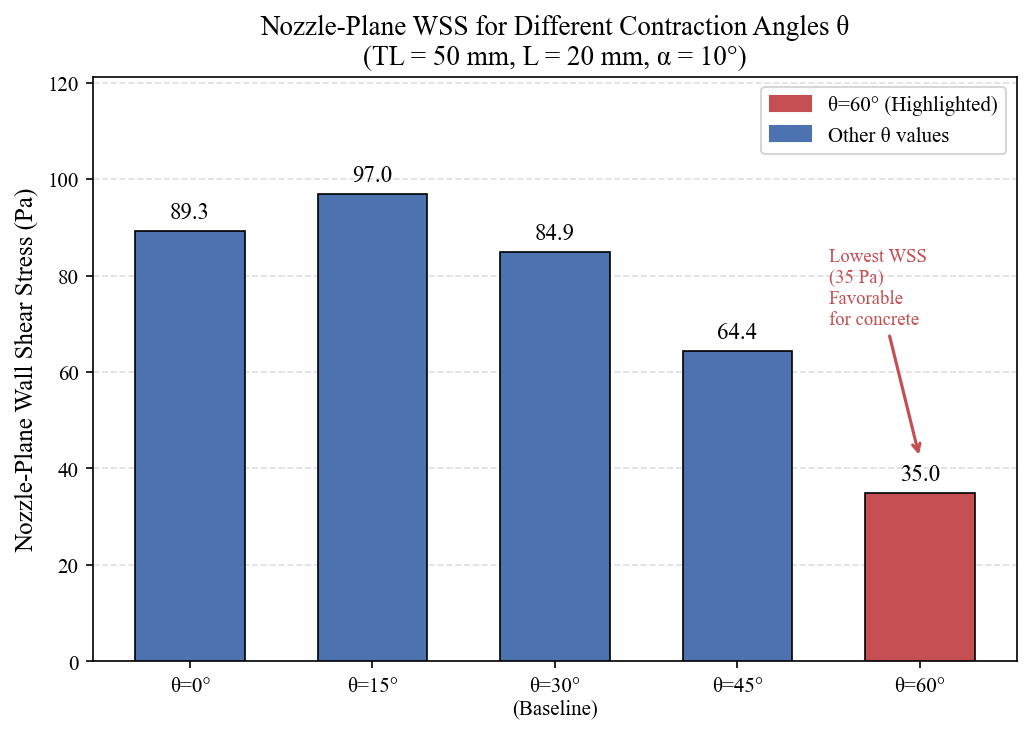
\includegraphics[width=0.75\textwidth]{figures/4.3.png}
  \caption{不同$\theta$工况下喷嘴出口处壁面剪切应力柱状对比图}
  \label{fig:4.3}
\end{figure}

\begin{figure}[!htb]
  \centering
  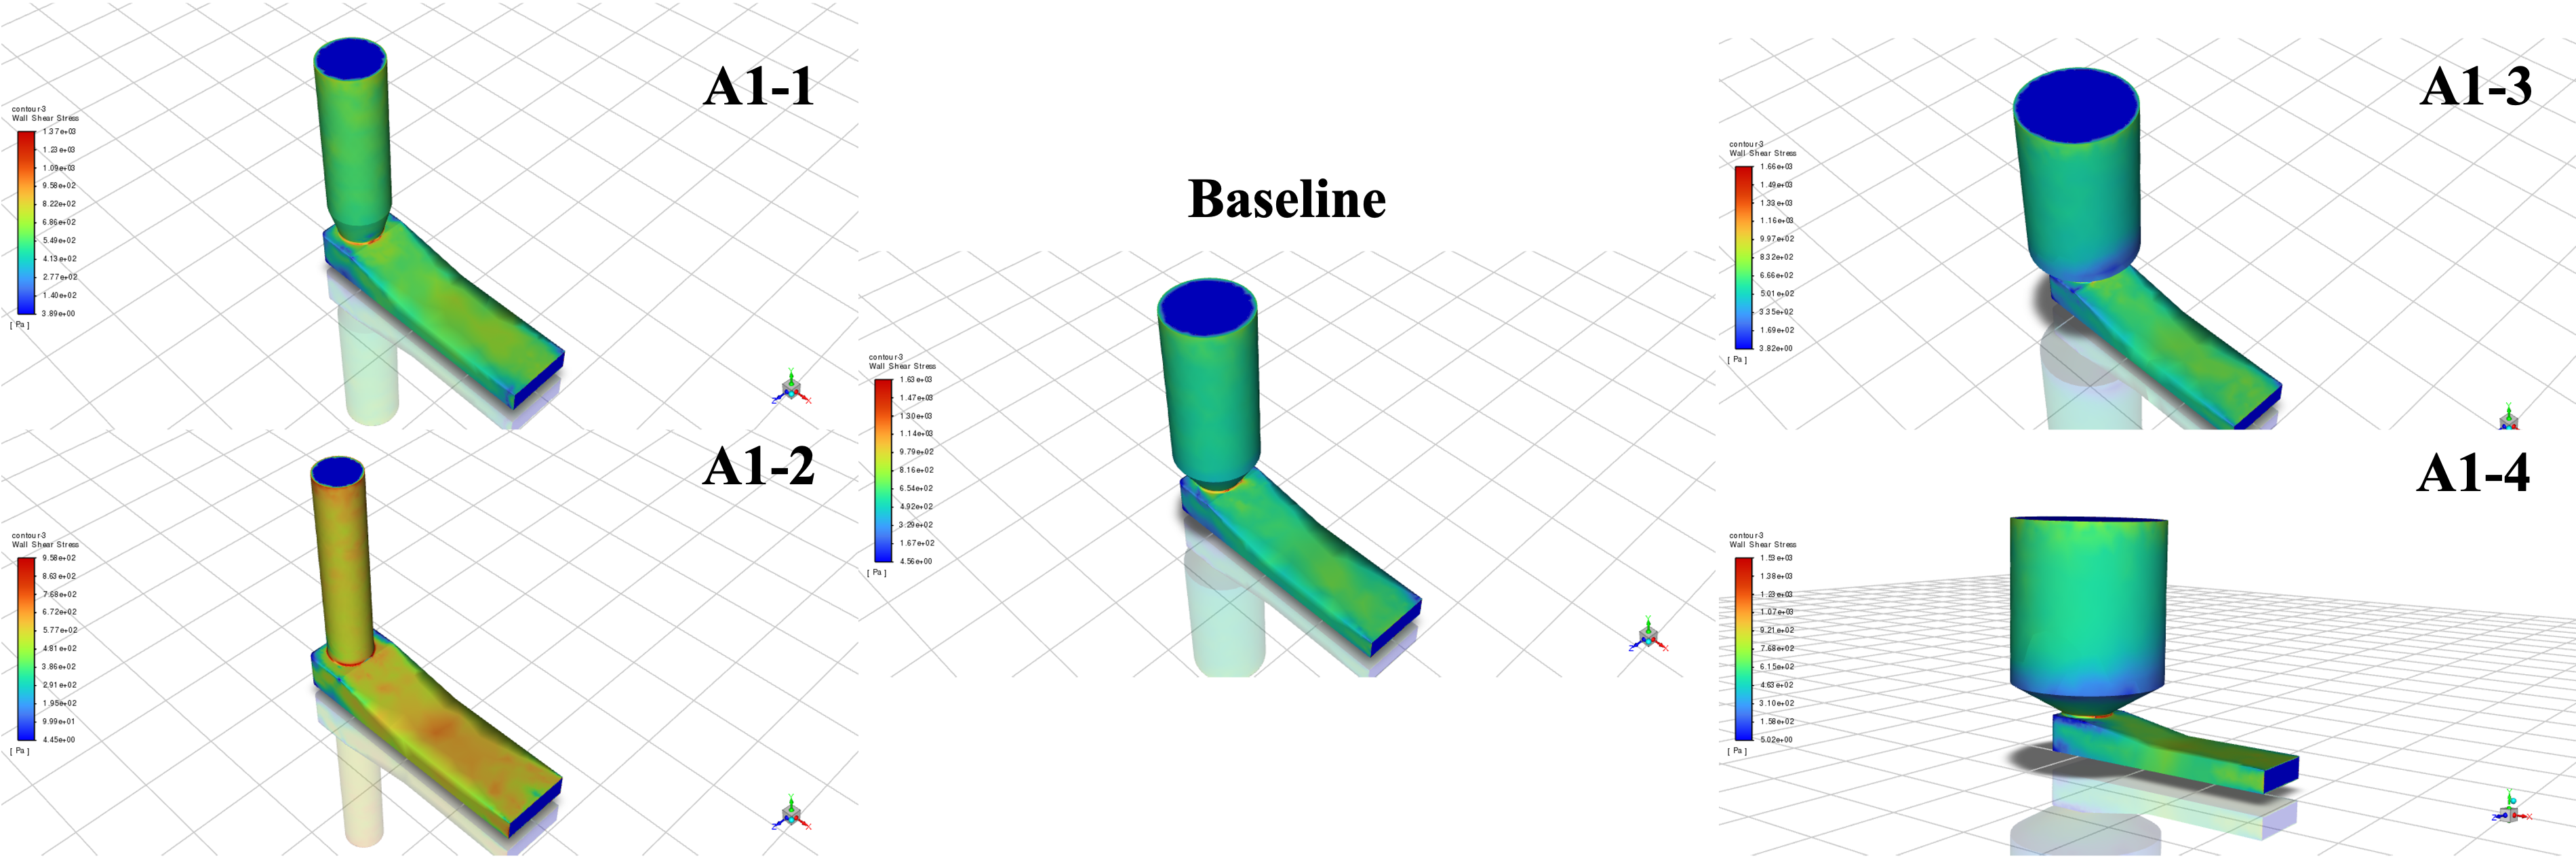
\includegraphics[width=0.9\textwidth]{figures/4.4.png}
  \caption{不同$\theta$下整体壁面剪切应力云图对比图}
  \label{fig:4.4}
\end{figure}

随$\theta$从0°增大至60°，$WSS_{nozzle}$呈现先升再减的趋势，从0°时的89.3~Pa短暂增加到15°时的97.0~Pa，随后单调降低至35.0~Pa，降幅达61\%。这一趋势与$P_{sub,AWA}$随$\theta$增大而先短暂降低后显著升高的规律方向相同，表明$\theta = 60°$是本研究中唯一能够同时提升基底接触压力（+19\%）并降低喷嘴壁面剪切应力（$-61\%$）的参数设置。这组工况在两个层面都展现出了出色的性能，是这组工况下最优的几何配置。

这一现象的物理机理可从剪切速率云图（\cref{fig:4.4}）中解释。收缩角较小时（如$\theta = 0°$或15°），喷嘴收缩段近壁区的速度梯度方向较为复杂，存在明显的流动分离趋势，导致面积加权平均后的剪切应力大小变化不大；而收缩角较大时（$\theta = 60°$），流线沿收缩壁面的曲率变化更为平滑，流动分离得到抑制，近壁速度梯度分布趋于均匀，局部高剪切区消失，整体壁面剪切载荷因此显著降低。

就工程设计角度而言，$\theta = 60°$时表现的出色的性能特征具有重要的实践意义。在保证其他几何参数不变的前提下，采用较大收缩角的喷嘴设计不仅能够提升层间粘结性能，还能延长喷嘴的磨损寿命，降低浆体在喷嘴内部受到的剪切损伤，是喷嘴几何优化的优先推荐方向。

\subsection{A1组工况综合评价}

综合以上讨论，随$\theta$增大，$P_{sub,AWA}$、$\eta_p$均提升，$WSS_{nozzle}$降低，三项指标均指向$\theta = 60°$为最优选择。唯一例外的是$UI$，在$\theta = 60°$时$UI = 1.84$，略高于其他工况。这说明在大收缩角工况下，基底面压力分布的空间均匀性略有下降，峰值压力区更为集中。$P_{inlet}$随$\theta$增大也略有上升，但相对于$P_{sub,AWA}$和$WSS_{nozzle}$的改善幅度而言代价较小。$\theta = 60°$（A1-4工况）为研究线A1的推荐参数，在后续C组优化工况中将采用该收缩角设置。

\section{喷嘴收缩段竖向长度$L$的影响（A2组工况）}

为研究喷嘴竖向高度对喷嘴挤出性能的影响，本组研究固定收缩角为30°，共选取4组工况进行了参数化研究。\cref{tab:4.3}总结了4组工况重点研究指标的结果。\cref{fig:4.5}展示了不同$L$工况下$P_{sub,AWA}$与$WSS_{outlet}$的对比柱状图。

\begin{table}[!htb]
  \centering
  \caption{A2组（$L$变化）各工况评价指标汇总表}\label{tab:4.3}
  \renewcommand{\arraystretch}{1.3}
  \begin{tabular}{lccccccl}
    \toprule
    \textbf{工况} & $L$ & $P_{sub}$(Pa) & $WSS_{nozzle}$ & $\eta_p$ & $UI$ & $P_{inlet}$ & \textbf{综合} \\
    \midrule
    A2-1     & 10 & 8323 & 80.7 & 0.428 & 1.74 & 202.2 & \\
    Baseline & 20 & 8310 & 84.9 & 0.421 & 1.78 & 172.7 & 基准 \\
    A2-2     & 30 & 8905 & 98.1 & 0.424 & 1.75 & 118.8 & \\
    A2-3     & 40 & 9382 & 81.9 & 0.422 & 1.70 & 178.0 & \\
    \bottomrule
  \end{tabular}
\end{table}

\begin{figure}[!htb]
  \centering
  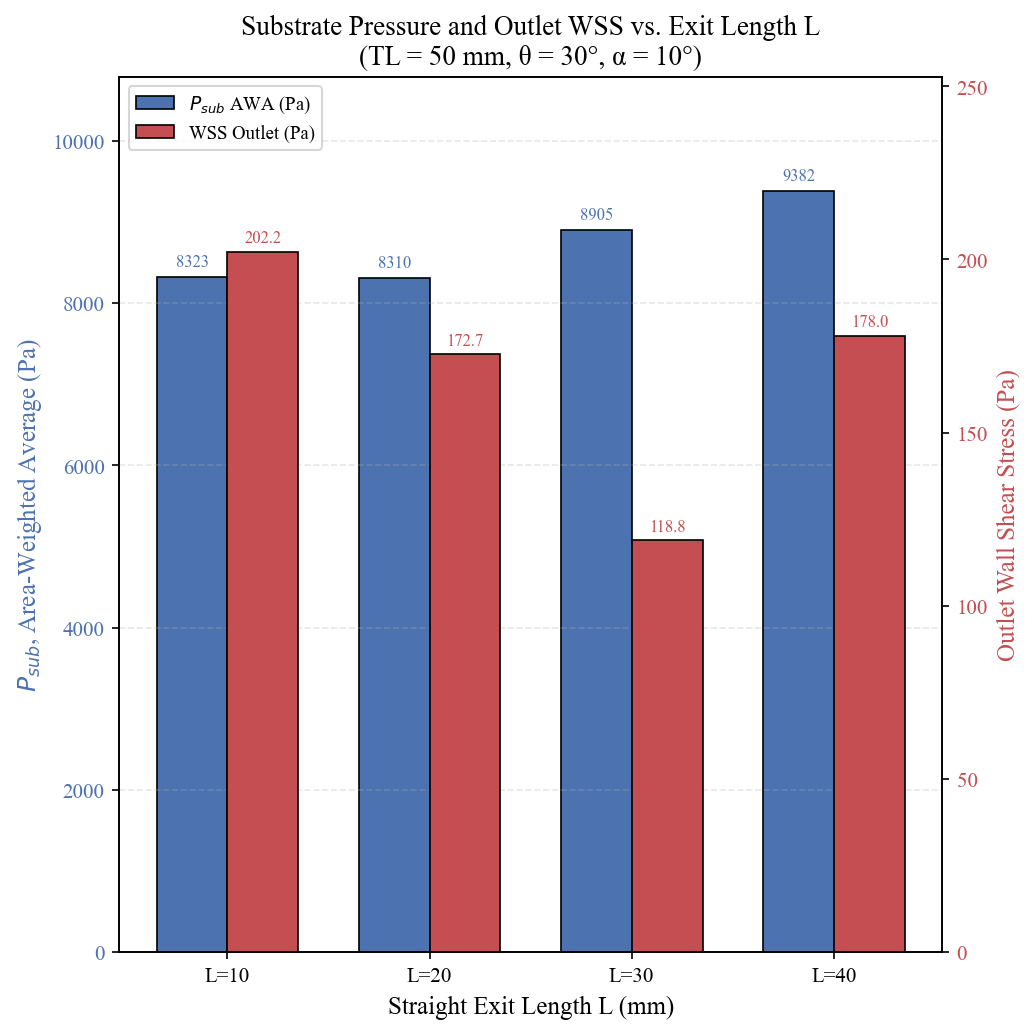
\includegraphics[width=0.8\textwidth]{figures/4.5.png}
  \caption{不同$L$下$P_{sub,AWA}$与$WSS_{outlet}$对比柱状图}
  \label{fig:4.5}
\end{figure}

由图可知，当高度$L$从10~mm增大至40~mm，$P_{sub,AWA}$从8323~Pa增至9382~Pa，增幅为+13\%。尽管变化趋势单调，但增幅相对有限，且数据点间的变化缺乏明显规律性，说明喷嘴收缩段竖向高度度对基底接触压力的调控能力较弱。

从物理机制来看，延长竖向高度主要增加了浆体在管道中的流动路程，对应更长的壁面摩擦损失路径，但由于出口面积不变，收缩段高度的增加不能像整形板那样通过改变流场几何形态来主动调控压力分布。收缩段高度的主要工程作用在于：为流体提供充分发展的速度剖面，确保进入整形板的流动状态稳定均匀。

$WSS_{outlet}$（整形板末端截面的壁面剪切应力）随$L$的变化呈现先降后升的非单调趋势，也反映了收缩段高度变化通过影响喷嘴出口速度剖面的充分发展程度，间接改变了整形板区域的局部流动状态。

总体来看，在本组对照试验的研究范围内（$L = 10$-40~mm），喷嘴收缩段竖向长度可视为对基底接触压力影响较小的次要参数，工程设计中可在满足制造约束的前提下灵活选取。

\section{整形板倾斜角$\alpha$的影响（B1组工况）}\label{sec:alpha-influence}

为研究整形板倾斜角度对喷嘴挤出性能的影响，本课题共选取5组工况进行了参数化研究。\cref{tab:4.4}总结了5组工况重点研究指标的结果。

\begin{table}[!htb]
  \centering
  \caption{B1组（$\alpha$变化）各工况评价指标汇总表}\label{tab:4.4}
  \renewcommand{\arraystretch}{1.3}
  \begin{tabular}{lcccccccc}
    \toprule
    \textbf{工况} & $\alpha$ & $H$(mm) & $P_{sub}$(Pa) & $WSS_{nozzle}$ & $\eta_p$ & $UI$ & $P_{inlet}$ \\
    \midrule
    B1-1     & 0°  & 22.00 & 5733  & 445.5 & 0.375 & 1.86 & 15274 \\
    B1-2     & 5°  & 17.64 & 6896  & 93.8  & 0.386 & 1.82 & 17856 \\
    Baseline & 10° & 13.32 & 8310  & 84.9  & 0.421 & 1.78 & 19750 \\
    B1-3     & 15° & 9.06  & 12081 & 77.1  & 0.481 & 1.64 & 25101 \\
    B1-4     & 20° & 4.90  & 22184 & 91.7  & 0.577 & 1.51 & 38418 \\
    \bottomrule
  \end{tabular}
\end{table}

\subsection{$\alpha$对基底压力的非线性影响}

\cref{fig:4.6}展示了$P_{sub,AWA}$随倾斜角$\alpha$变化的关系曲线，\cref{fig:4.7}和\cref{fig:4.8}分别展示了不同$\alpha$工况下的基底压力云图与速度流线对比。

\begin{figure}[!htb]
  \centering
  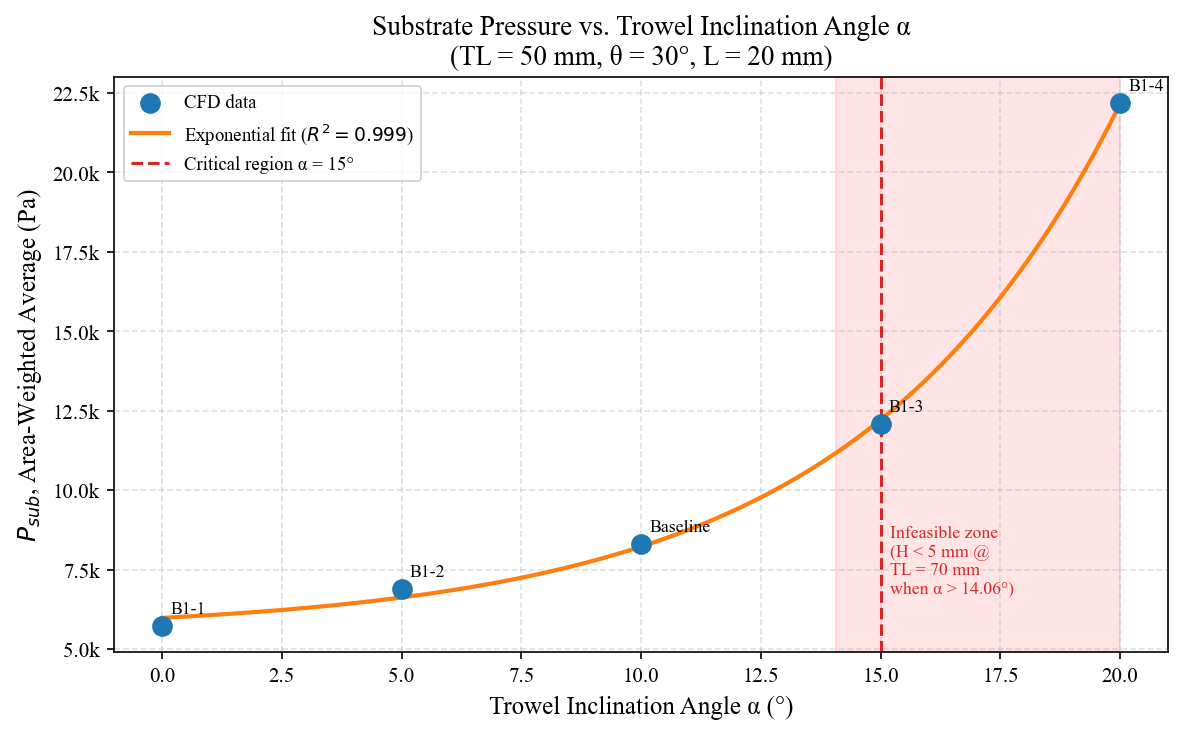
\includegraphics[width=0.75\textwidth]{figures/4.6.png}
  \caption{$P_{sub,AWA}$--$\alpha$关系曲线}
  \label{fig:4.6}
\end{figure}

\begin{figure}[!htb]
  \centering
  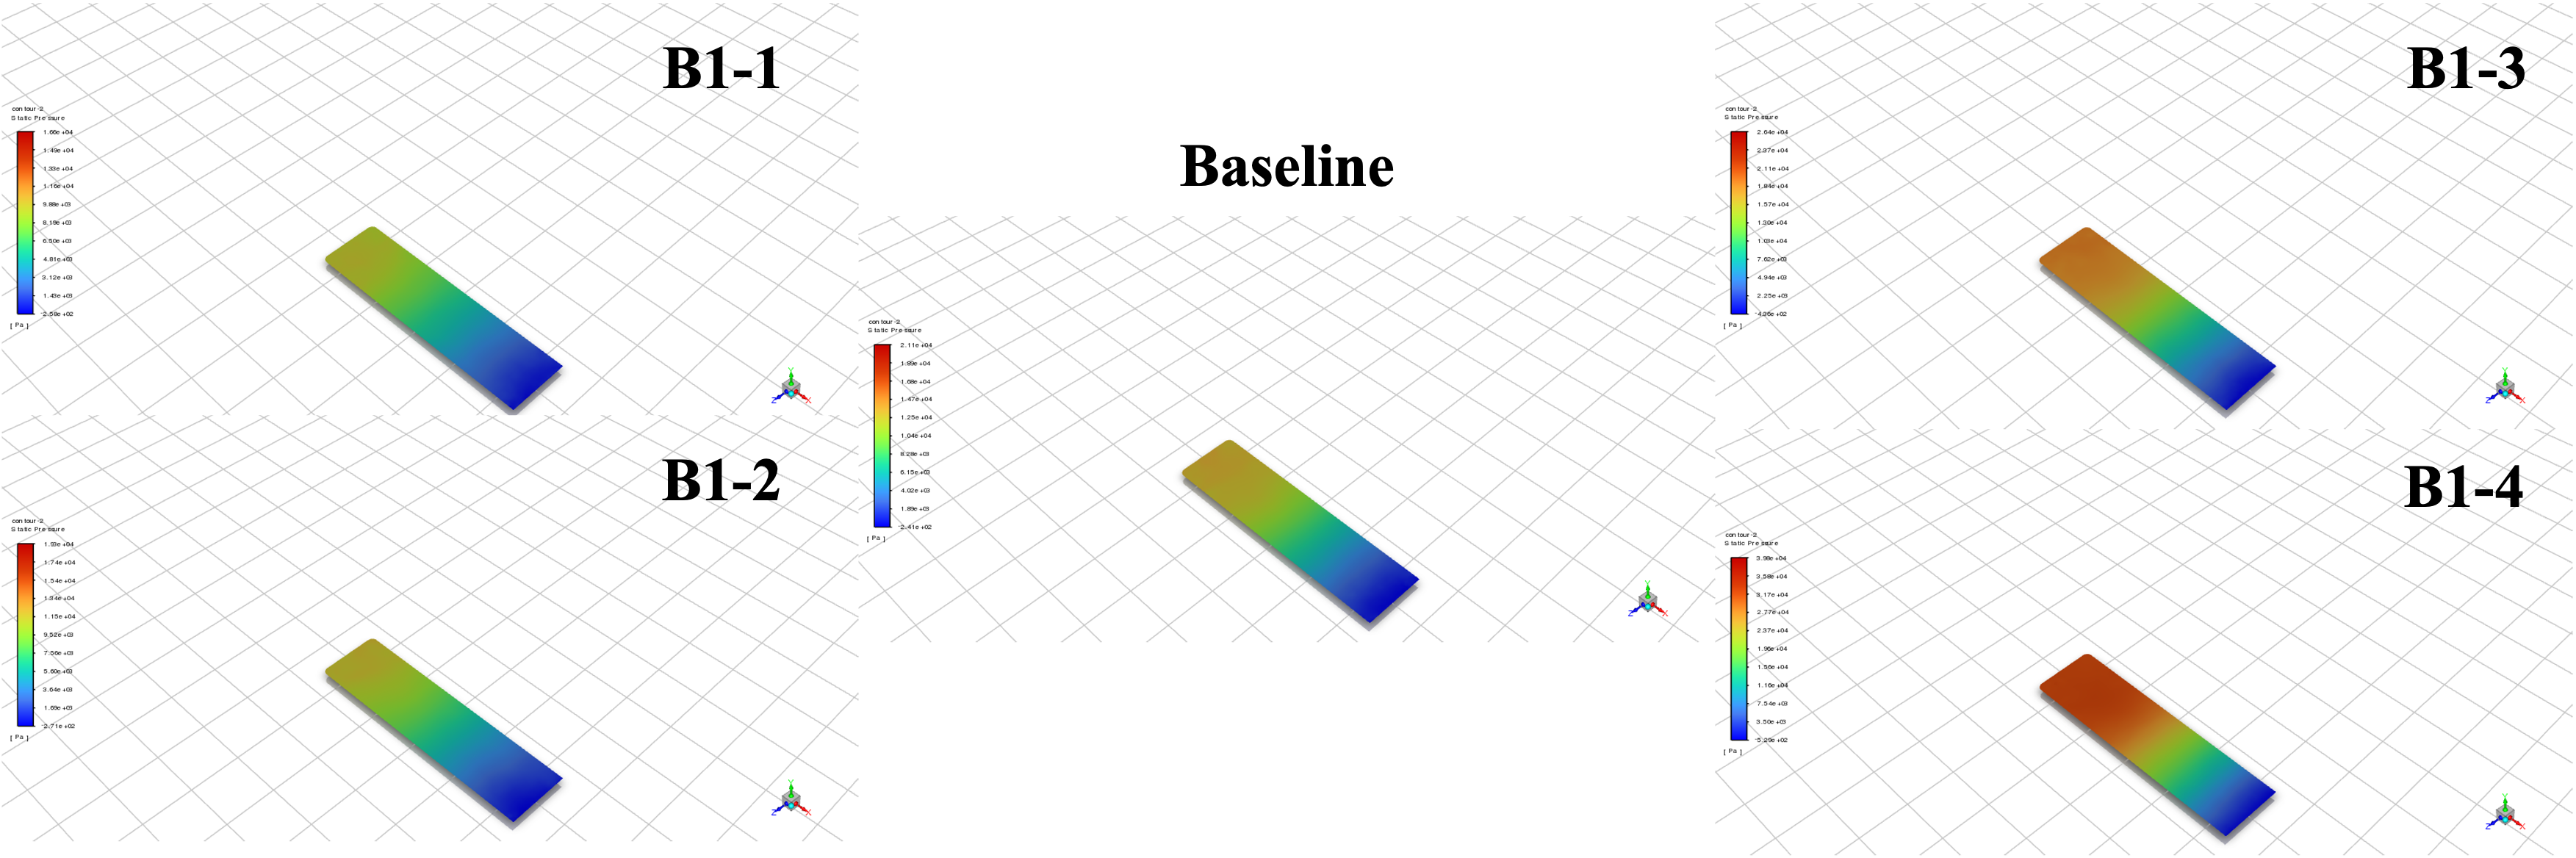
\includegraphics[width=0.9\textwidth]{figures/4.7.png}
  \caption{不同$\alpha$下基底压力云图对比图}
  \label{fig:4.7}
\end{figure}

\begin{figure}[!htb]
  \centering
  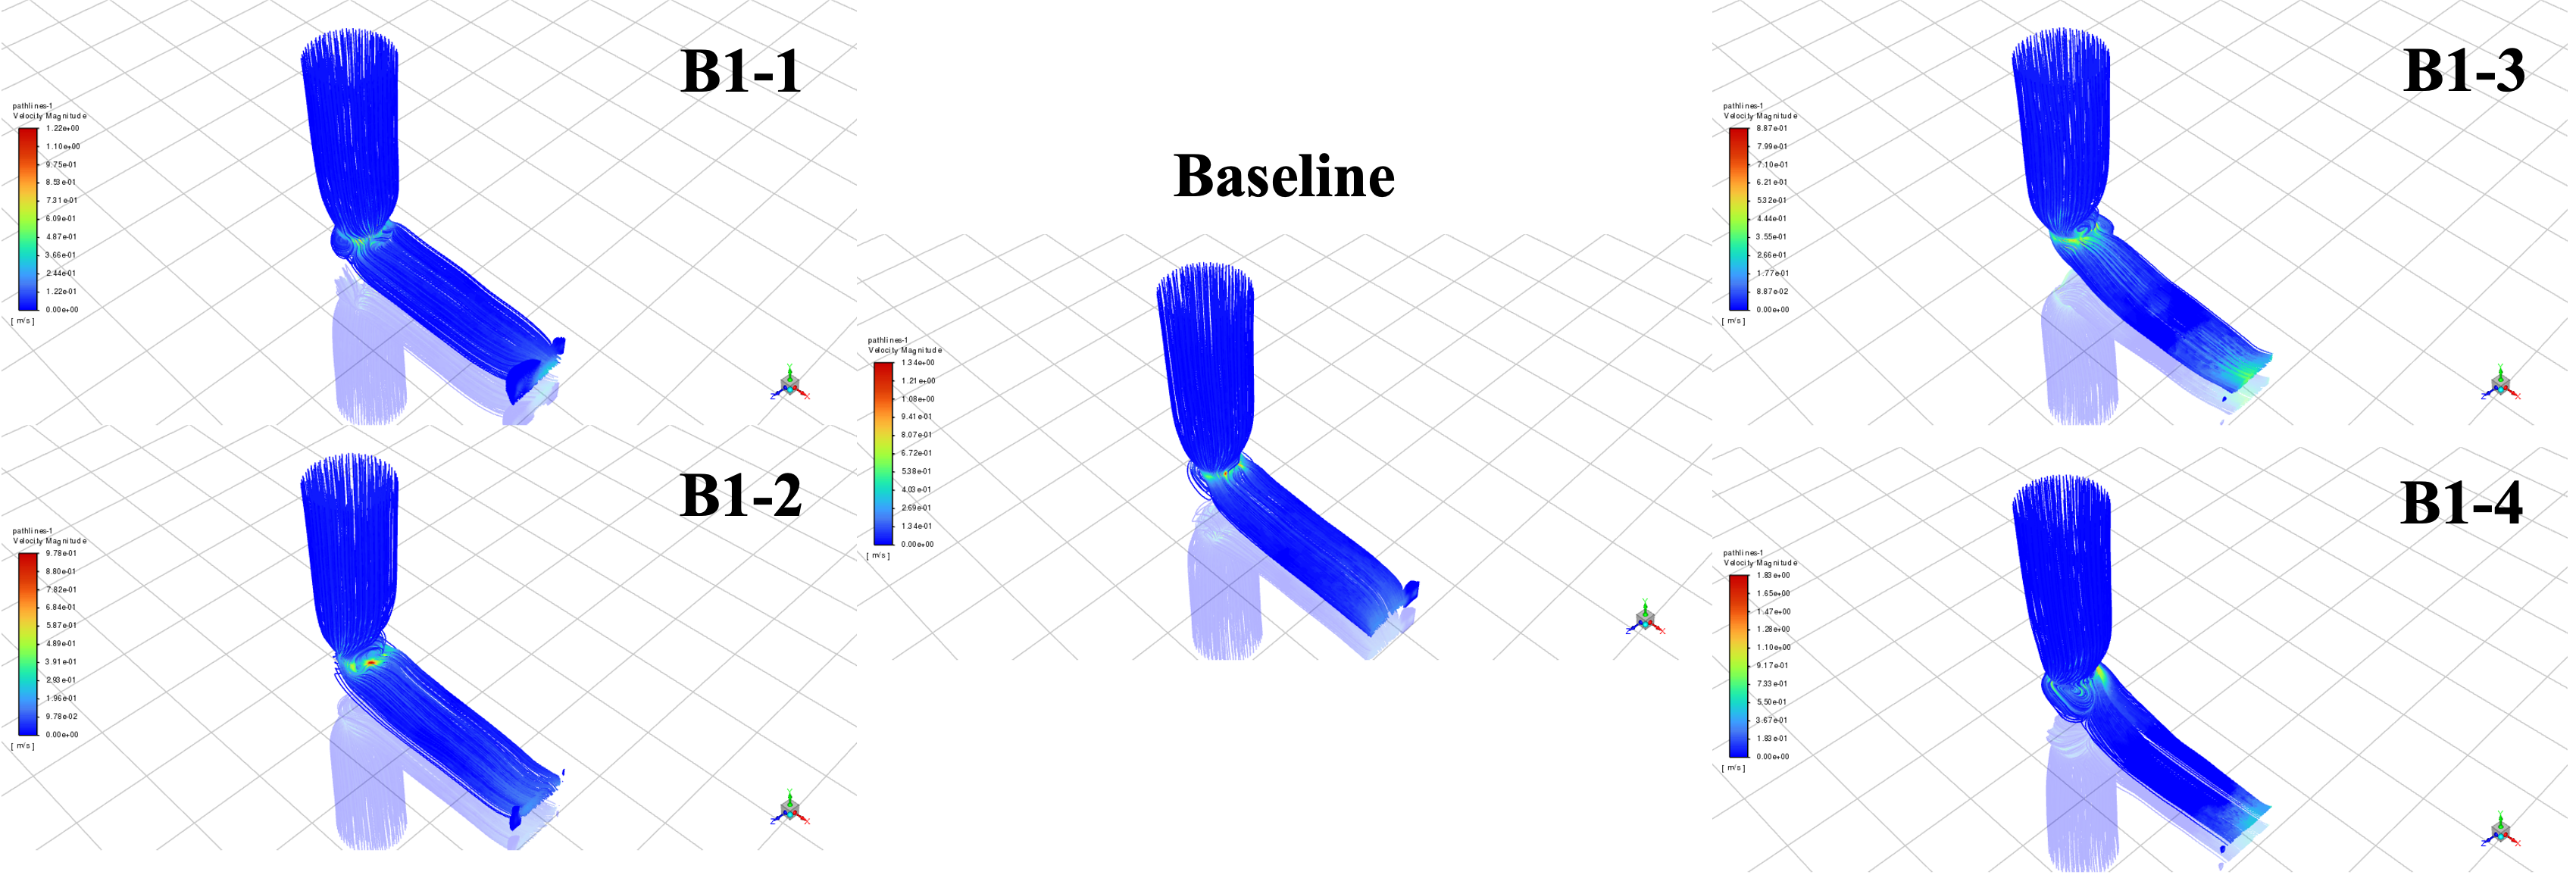
\includegraphics[width=0.9\textwidth]{figures/4.8.png}
  \caption{不同$\alpha$下速度流线对比图}
  \label{fig:4.8}
\end{figure}

结果表明，$\alpha$是本研究四个设计变量中对基底接触压力影响最为显著的参数。$\alpha$从0°增大至20°，$P_{sub,AWA}$从5733~Pa增至22184~Pa，增幅高达287\%。值得注意的是，该增长过程并非线性：在$\alpha \leq 15°$范围内，压力随$\alpha$的增大较为平稳；而在$\alpha$从15°增至20°时，压力出现非线性激增（12081~Pa$\to$22184~Pa，单步增幅+84\%），呈现明显的临界加速行为。

这一非线性现象的物理根源在于整形板出口处的楔形流动效应。由\cref{eq:H}给出的定量关系可知：随$\alpha$增大，整形板倾斜面与基底面之间形成的楔形通道出口间隙$H$（即层高）不断减小。在楔形受限流动中，压力增益与间隙高度的平方成反比，可由Reynolds楔形润滑方程近似描述，方程简化后形式为：
\begin{equation}\label{eq:wedge}
  \Delta P_{wedge} \approx \frac{6 \eta v \cdot L_{eff}}{h^2},
\end{equation}
其中$\eta$为浆体表观黏度，$v$为出料口流速，$L_{eff}$为楔形约束有效长度，$h$为出口间隙高度。由该式可见，当$h$减小时，$\Delta P_{wedge}$以$h^{-2}$的速率增大，间隙越小，压力增益越剧烈，这直接解释了$\alpha$从15°到20°时基底压力的非线性激增现象。

由\cref{eq:dH-dalpha}几何关系可知，层高$H$对$\alpha$的偏导数为$\partial H / \partial \alpha = -TL \cos(\alpha) < 0$，表明层高$H$随$\alpha$单调递减。随$\alpha$增大，楔形效应增强，基底压力迅速上升，但层高$H$同步减小，在$\alpha$超过可行性阈值后，沉积层过薄将无法保证打印质量，这构成了$\alpha$参数优化的核心约束，也说明整形板倾斜角的大小需要在保证打印层高度允许范围之内进行优化分析处理。

当$\alpha = 0°$时（工况B1-1），整形板出料段水平，不形成楔形约束，浆体在出料口处自由扩散，$WSS_{nozzle}$高达445.5~Pa，远超其他工况的5倍以上。这一异常高剪切应力源于$\alpha = 0°$时喷嘴出口流体在无约束条件下发生剧烈的方向转折，在前挡板附近产生强烈的回流涡和局部高速梯度区。

由于工况B1-1的截面壁面剪切应力数据偏离正常分布范围，将其纳入代理模型训练集会严重破坏模型的拟合质量，因此在后续的响应面建模中，B1-1并没有纳入相关模型的训练集，但其$P_{sub,AWA}$数据仍作为$\alpha = 0°$时的极限对照保留。

\subsection{$\alpha$与层高约束的解析关系}

层高约束$H \geq 5$~mm是本研究对$\alpha$参数设置的几何限制条件之一。由\cref{eq:H}反函数推导后，可得$\alpha$的可行上界：
\begin{equation}\label{eq:alpha-max}
  \alpha_{max} = \arcsin\left( \frac{Z_0 - H_{min}}{TL} \right).
\end{equation}
\cref{fig:4.9}展示了在$TL = 30, 40, 50, 60, 70$~mm五种整形板长度下，层高$H$随$\alpha$变化的曲线族。绿色区域（$H \geq 5$~mm）为几何可行域，红色区域（$H < 5$~mm）为不可行域。由图可见，当$TL$较大时，$\alpha$的可行范围更窄：$TL = 70$~mm时，$\alpha_{max} = \arcsin(17/70) = 14.06°$，而$TL = 30$~mm时，$\alpha_{max} = \arcsin(17/30) = 34.6°$。

B1-4工况（$\alpha = 20°$，$TL = 50$~mm）对应层高$H = 22 - 50 \times \sin(20°) = 4.90$~mm$< 5$~mm，不满足层高约束，虽然其$P_{sub,AWA} = 22184$~Pa为所有B1组工况最高，但因几何不可行而被排除出Pareto优化的可行域。在追求高接触压力的同时，层高约束是不可逾越的工程边界，优化设计必须在可行域内进行。

\begin{figure}[!htb]
  \centering
  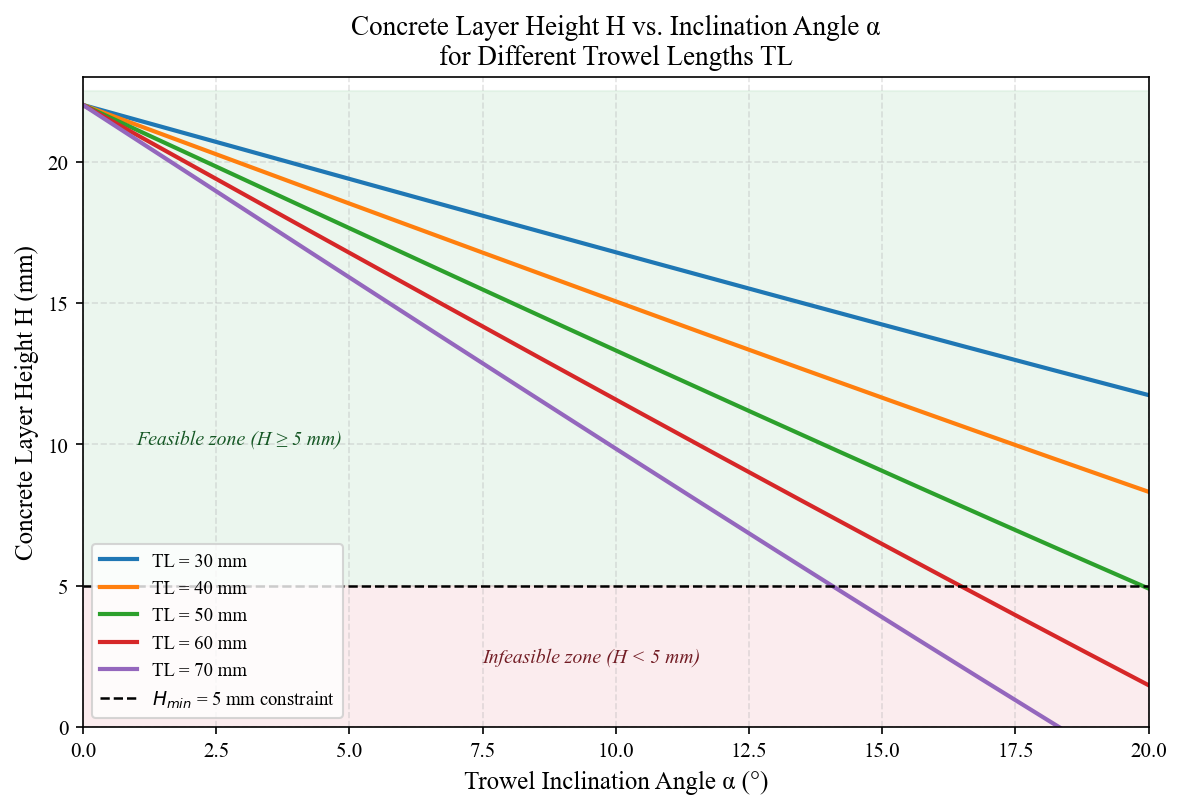
\includegraphics[width=0.8\textwidth]{figures/4.9.png}
  \caption{层高$H$与$\alpha$的关系图}
  \label{fig:4.9}
\end{figure}

\subsection{B1组工况综合评价}

综上所述，在满足层高约束的工况中，B1-3（$\alpha = 15°$）的综合性能最优：$P_{sub,AWA} = 12081$~Pa（较Baseline提升+45\%），$\eta_p = 0.481$（较Baseline提升+14\%），$UI = 1.64$（低于Baseline的1.78，压力均匀性改善）。尽管B1-3的$P_{inlet} = 25101$~Pa较Baseline高出27\%，但考虑到$P_{sub,AWA}$的大幅提升，压力传递效率的整体提高是值得的。B1-3的参数设置（$\alpha = 15°$）将在C组优化工况中被采用，与$\theta = 60°$的喷嘴参数组合，验证参数协同效应。

\section{整形板延伸长度$TL$的影响（B2组工况）}

为研究整形板延伸长度对喷嘴挤出性能的影响，本组研究固定整形板倾斜角为10°，共选取5组工况进行了参数化研究。\cref{tab:4.5}总结了5组工况重点研究指标的结果。\cref{fig:4.10}展示了$P_{sub,AWA}$随$TL$变化的折线图，\cref{fig:4.11}展示了五种$TL$工况下的基底压力云图对比，\cref{fig:4.12}展示了不同整形板延伸长度下基底面压力沿打印方向（X轴）分布曲线的叠加图。

\begin{table}[!htb]
  \centering
  \caption{B2组（$TL$变化）各工况评价指标汇总表}\label{tab:4.5}
  \renewcommand{\arraystretch}{1.3}
  \begin{tabular}{lcccccccc}
    \toprule
    \textbf{工况} & $TL$(mm) & $H$(mm) & $P_{sub}$(Pa) & $WSS_{nozzle}$ & $\eta_p$ & $UI$ & $P_{inlet}$ \\
    \midrule
    B2-1     & 30 & 16.79 & 5944  & 86.6  & 0.365 & 1.83 & 16277 \\
    B2-2     & 40 & 15.05 & 7177  & 81.0  & 0.390 & 1.79 & 18390 \\
    Baseline & 50 & 13.32 & 8310  & 84.9  & 0.421 & 1.78 & 19750 \\
    B2-3     & 60 & 11.58 & 10353 & 82.0  & 0.451 & 1.73 & 22937 \\
    B2-4     & 70 & 9.85  & 12833 & 102.1 & 0.483 & 1.68 & 26549 \\
    \bottomrule
  \end{tabular}
\end{table}

\begin{figure}[!htb]
  \centering
  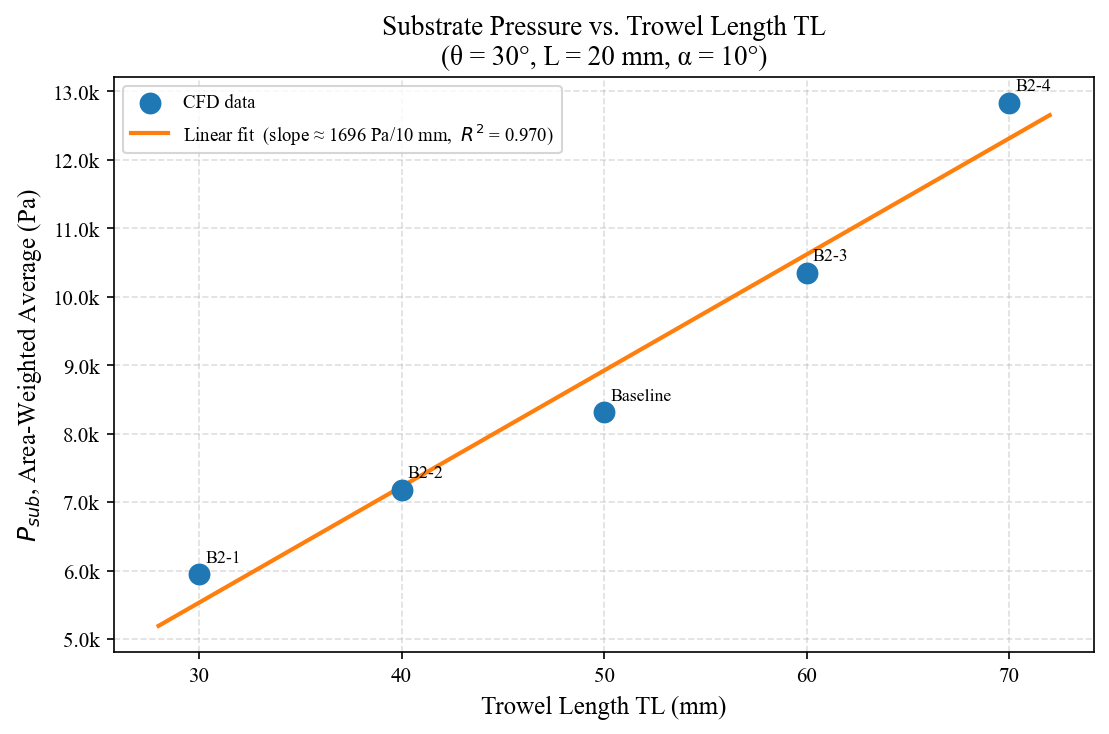
\includegraphics[width=0.75\textwidth]{figures/4.10.png}
  \caption{$P_{sub,AWA}$--$TL$折线图}
  \label{fig:4.10}
\end{figure}

\begin{figure}[!htb]
  \centering
  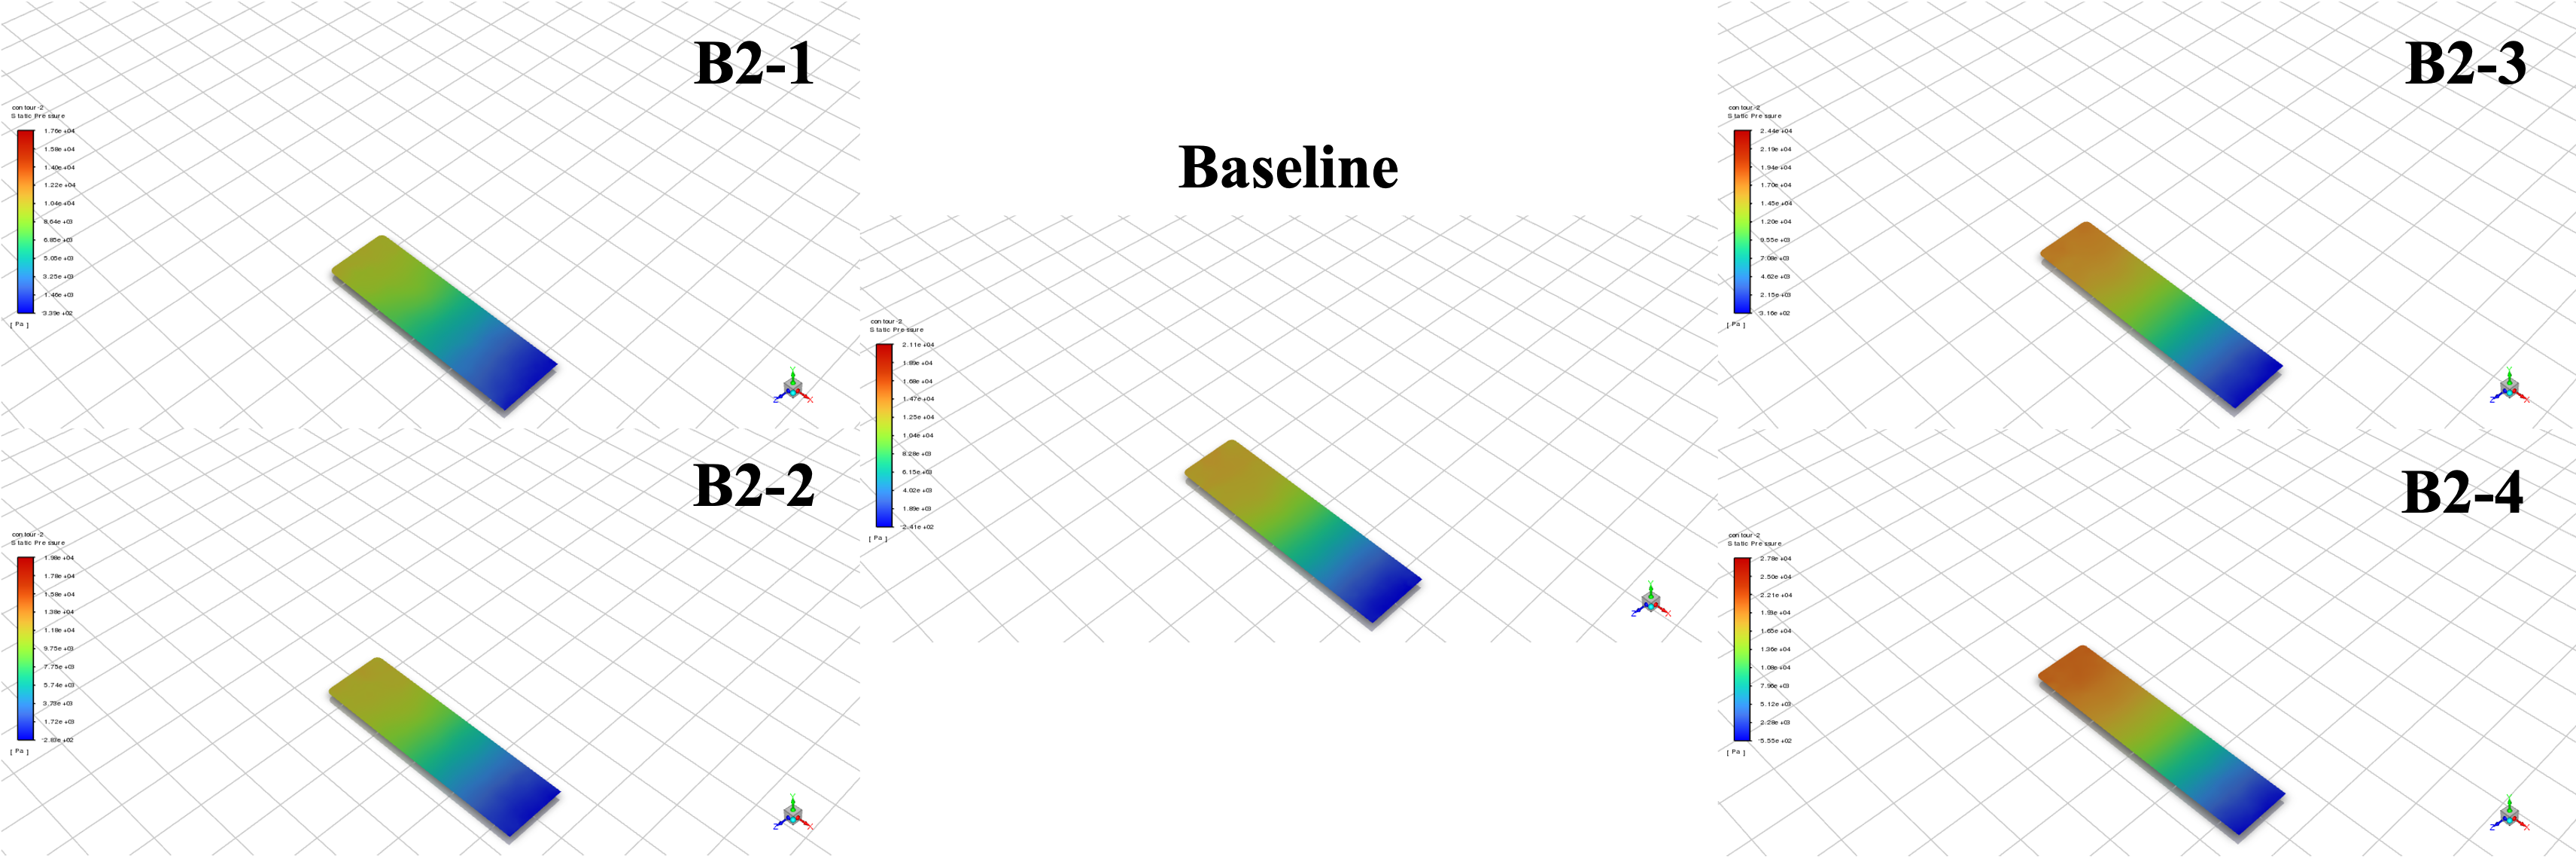
\includegraphics[width=0.9\textwidth]{figures/4.11.png}
  \caption{不同$TL$下基底压力云图对比图}
  \label{fig:4.11}
\end{figure}

\begin{figure}[!htb]
  \centering
  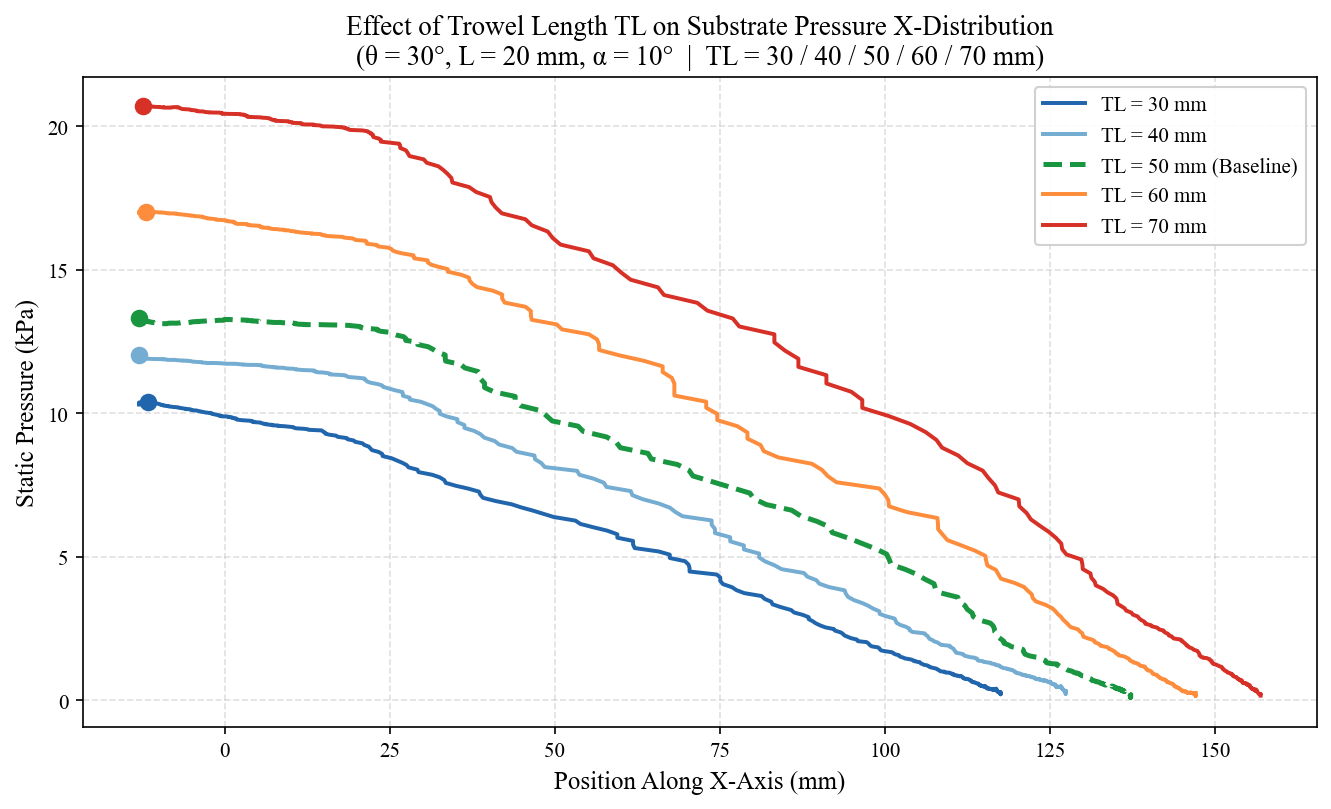
\includegraphics[width=0.8\textwidth]{figures/4.12.png}
  \caption{$TL$对基底压力XY分布曲线的影响图}
  \label{fig:4.12}
\end{figure}

由\cref{fig:4.10}可以看出，当$TL$从30~mm增大至70~mm，$P_{sub,AWA}$从5944~Pa增至12833~Pa，增幅为+116\%，Pearson相关系数$r = 0.541$（$p = 0.014$），具有统计显著性。线性拟合结果表明，$TL$每增加10~mm，$P_{sub,AWA}$约增加1700~Pa，两者近似呈线性正相关关系（$R^2 = 0.999$）。

从\cref{fig:4.12}的压力XY曲线叠加图中，可以清晰观察到整形板延伸长度影响的空间分布特征：随延伸长度增大，基底面压力的峰值不断升高，且高压区域沿打印方向（+X方向）的覆盖范围持续扩展，压力影响区域的范围随整形板的延伸而同步增大。这一空间扩展效应说明，$TL$的作用机制与$\alpha$有所不同：$\alpha$主要通过缩小出口间隙来增强楔形压力，而$TL$主要通过延长约束接触长度来积累压力。

从物理机理而言，更长的整形板提供了更长的流体约束路径，使浆体在受限空间内的停留时间更长，约束面对浆体施加压力的面积也更大，从而使总接触力显著提升。此外，由\cref{fig:4.12}还可得出：$TL$增大后整形板末端负压区的幅值略有增大，这是因为更长的整形板在末端产生更强的流动释放效应，局部分离更为明显。

与$\alpha$参数相比，$TL$是一种更为温和的增压手段。在相同的$P_{sub,AWA}$提升幅度下，通过增大$TL$所消耗的层高余量远小于通过增大$\alpha$：$TL = 70$~mm时层高仍有$H = 9.85$~mm（安全余量充足），而$\alpha = 15°$时层高已降至9.06~mm。因此，在工程实际中，优先通过增大$TL$来提升接触压力，以$\alpha$作为精细调节手段，是兼顾性能与安全余量的合理策略。

\section{优化工况组C分析}

\subsection{参数协同效应验证（C1组工况）}

基于研究线A和B的单因素分析结论，C1组工况通过将最优参数组合来探索参数间的协同增强效应。C1组共包含三组工况，其中C1-1与A1-4完全相同（$TL = 50$~mm，$\theta = 60°$，$\alpha = 10°$），代表A组工况下最大喷嘴收缩角带来的协同优化效应；C1-2（$TL = 55$~mm，$\theta = 30°$，$\alpha = 15°$）在保持喷嘴参数不变的条件下，仅对整形板参数进行优化，$P_{sub,AWA} = 14525$~Pa，较Baseline提升+75\%；C1-3（$TL = 60$~mm，$\theta = 60°$，$\alpha = 15°$）在C1-2的基础上同时将收缩角提升至$\theta = 60°$，$P_{sub,AWA} = 21677$~Pa，较Baseline提升+161\%。\cref{tab:4.6}总结了这三组工况的重点研究指标的结果，\cref{fig:4.13}展示了前四优化指标与基线水平的柱状对比图。

\begin{table}[!htb]
  \centering
  \caption{C1组（协同效应组）各工况评价指标汇总表}\label{tab:4.6}
  \renewcommand{\arraystretch}{1.3}
  \begin{tabular}{lcccccccc}
    \toprule
    \textbf{工况} & $TL$ & $\theta$ & $L$ & $\alpha$ & $P_{sub}$(Pa) & $WSS_{nozzle}$ & $\eta_p$ & $UI$ \\
    \midrule
    Baseline & 50 & 30 & 20 & 10 & 8310  & 84.9  & 0.421 & 1.78 \\
    C1-1     & 50 & 60 & 20 & 10 & 9926  & 35.00 & 0.447 & 1.84 \\
    C1-2     & 55 & 30 & 20 & 15 & 14525 & 74.66 & 0.506 & 1.64 \\
    C1-3     & 60 & 60 & 20 & 15 & 21677 & 41.07 & 0.557 & 1.58 \\
    \bottomrule
  \end{tabular}
\end{table}

\begin{figure}[!htb]
  \centering
  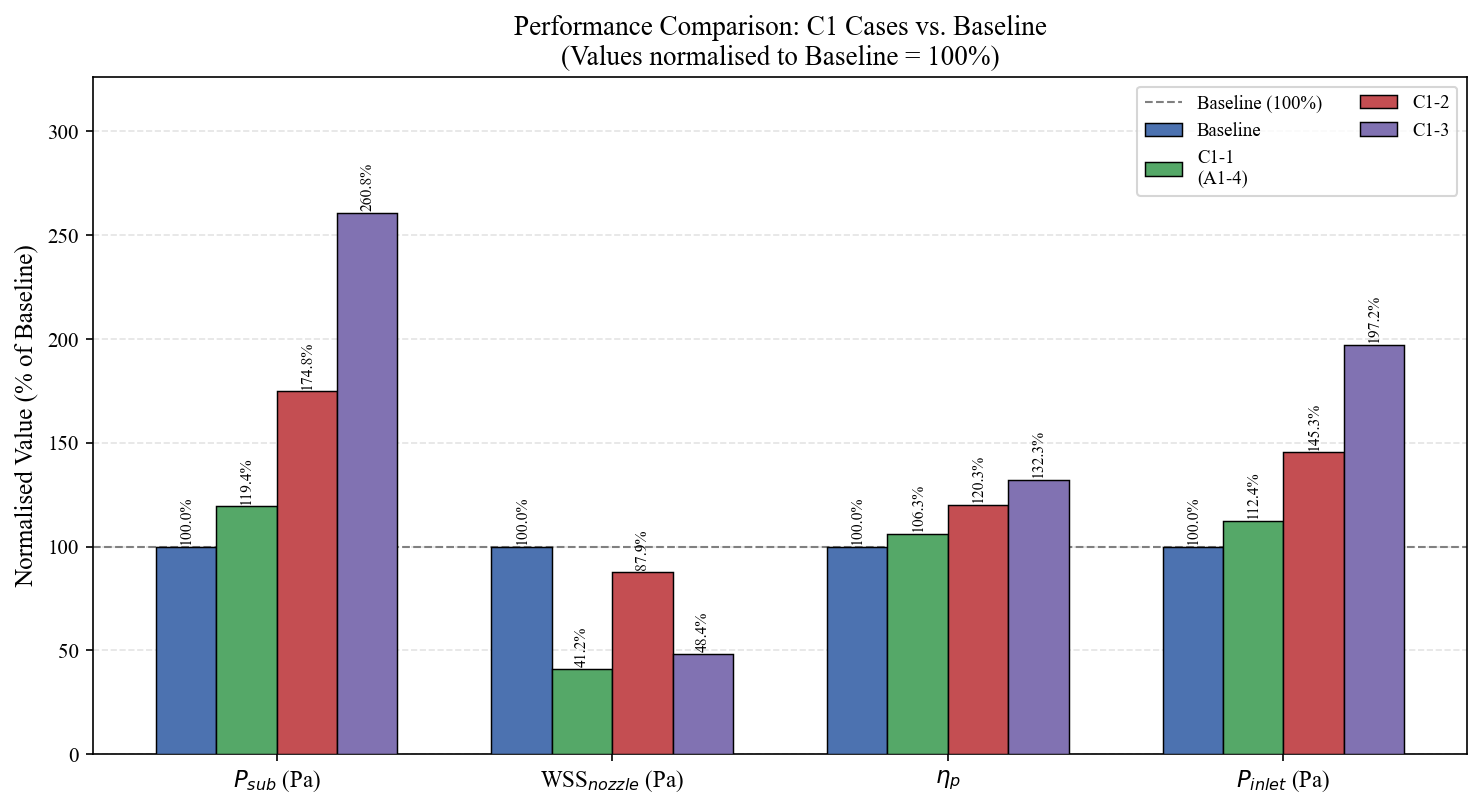
\includegraphics[width=0.85\textwidth]{figures/4.13.png}
  \caption{C1组别四优化指标与基线水平的柱状对比图}
  \label{fig:4.13}
\end{figure}

值得重点关注的是，C1-3的提升幅度（+161\%）显著超过了A1-4（仅优化$\theta$，+19\%）与C1-2（仅优化整形板，+75\%）两者效果的简单叠加（+94\%）。这一效应表明，喷嘴收缩角$\theta = 60°$与整形板参数$\alpha = 15°$、$TL = 60$~mm之间存在正向协同放大机制：大收缩角使喷嘴出口流体具有更高的动压和更均匀的速度剖面，当这一高动压流体进入由较大$\alpha$和较长$TL$所形成的强楔形约束空间时，楔形效应对高动压流体的压力转化效率更高，两种效应相互增强，产生超线性的压力增益。\cref{fig:4.14}中的基底压力XY分布叠加曲线直观展示了这一协同效应：C1-3（$\theta = 60°$，$\alpha = 15°$）的压力分布曲线不仅峰值最高，覆盖范围也最广，明显优于同$\alpha$但$\theta = 30°$的B1-3工况。

\begin{figure}[!htb]
  \centering
  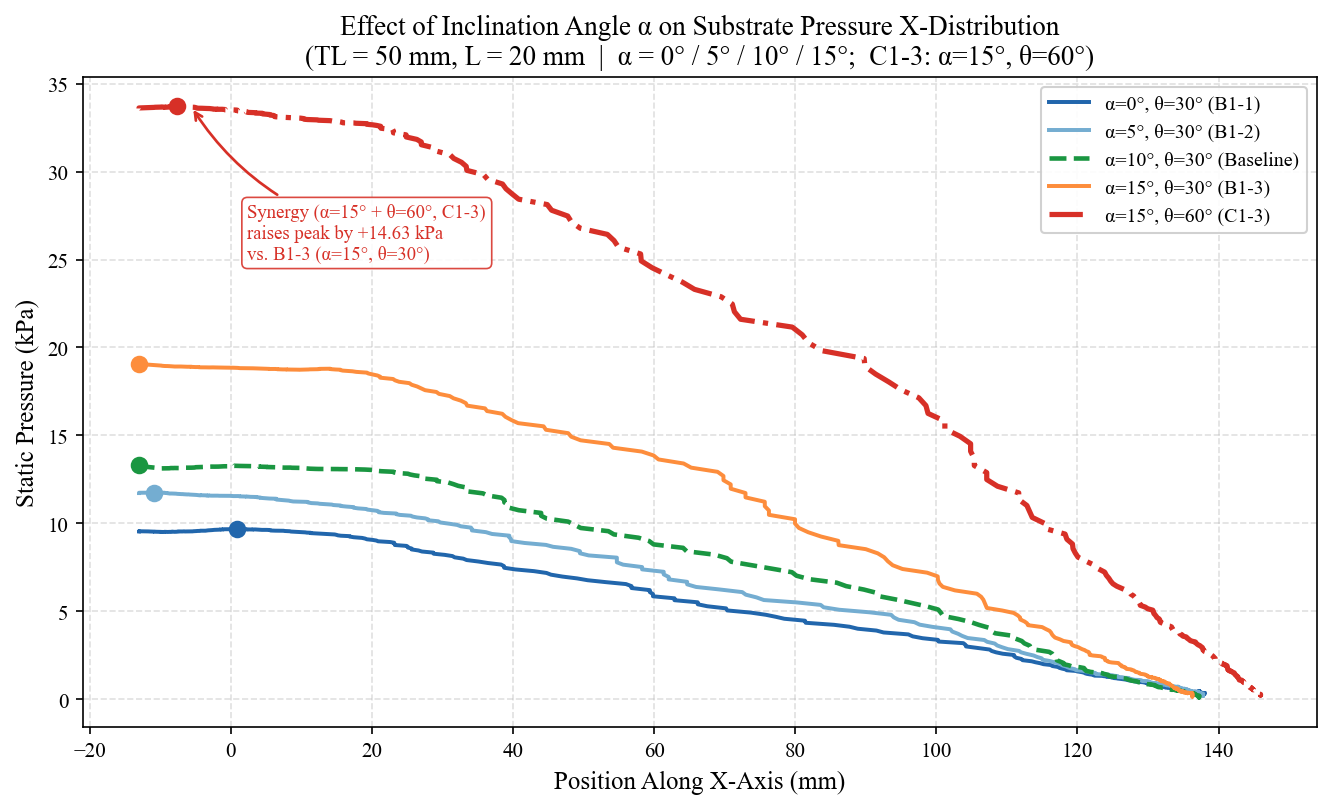
\includegraphics[width=0.8\textwidth]{figures/4.14.png}
  \caption{不同参数组合下基底面压力XY分布曲线叠加图}
  \label{fig:4.14}
\end{figure}

\subsection{无顶板整形板对照分析（C2工况）}

C2组工况作为对比试验验证整形板这一元件对混凝土打印浆体基础的正向效应。C2工况去除了整形板顶板，仅保留前挡板与75~mm延伸段，整形板出口平面已不存在，定义在喷嘴出口平面+X向坐标最大点处切线所在的ZY平面上；压力释放口仍然定义在延伸段出口所在平面。\cref{tab:4.7}总结了C2工况与基础工况的重点研究指标结果对比。结果表明，C2工况的$P_{sub,AWA} = 3436$~Pa，为全部20个工况中最低，较Baseline大幅降低59\%。

\begin{table}[!htb]
  \centering
  \caption{C2工况评价指标对比表}\label{tab:4.7}
  \renewcommand{\arraystretch}{1.3}
  \begin{tabular}{lcccccccc}
    \toprule
    \textbf{工况} & $TL$ & $\theta$ & $L$ & $\alpha$ & $P_{sub}$(Pa) & $WSS_{nozzle}$ & $\eta_p$ & $UI$ \\
    \midrule
    Baseline & 50  & 30 & 20 & 10 & 8310 & 84.9 & 0.421 & 1.78 \\
    C2       & --- & 30 & 20 & ---& 3436 & 382  & 0.300 & 2.09 \\
    \bottomrule
  \end{tabular}
\end{table}

\begin{figure}[!htb]
  \centering
  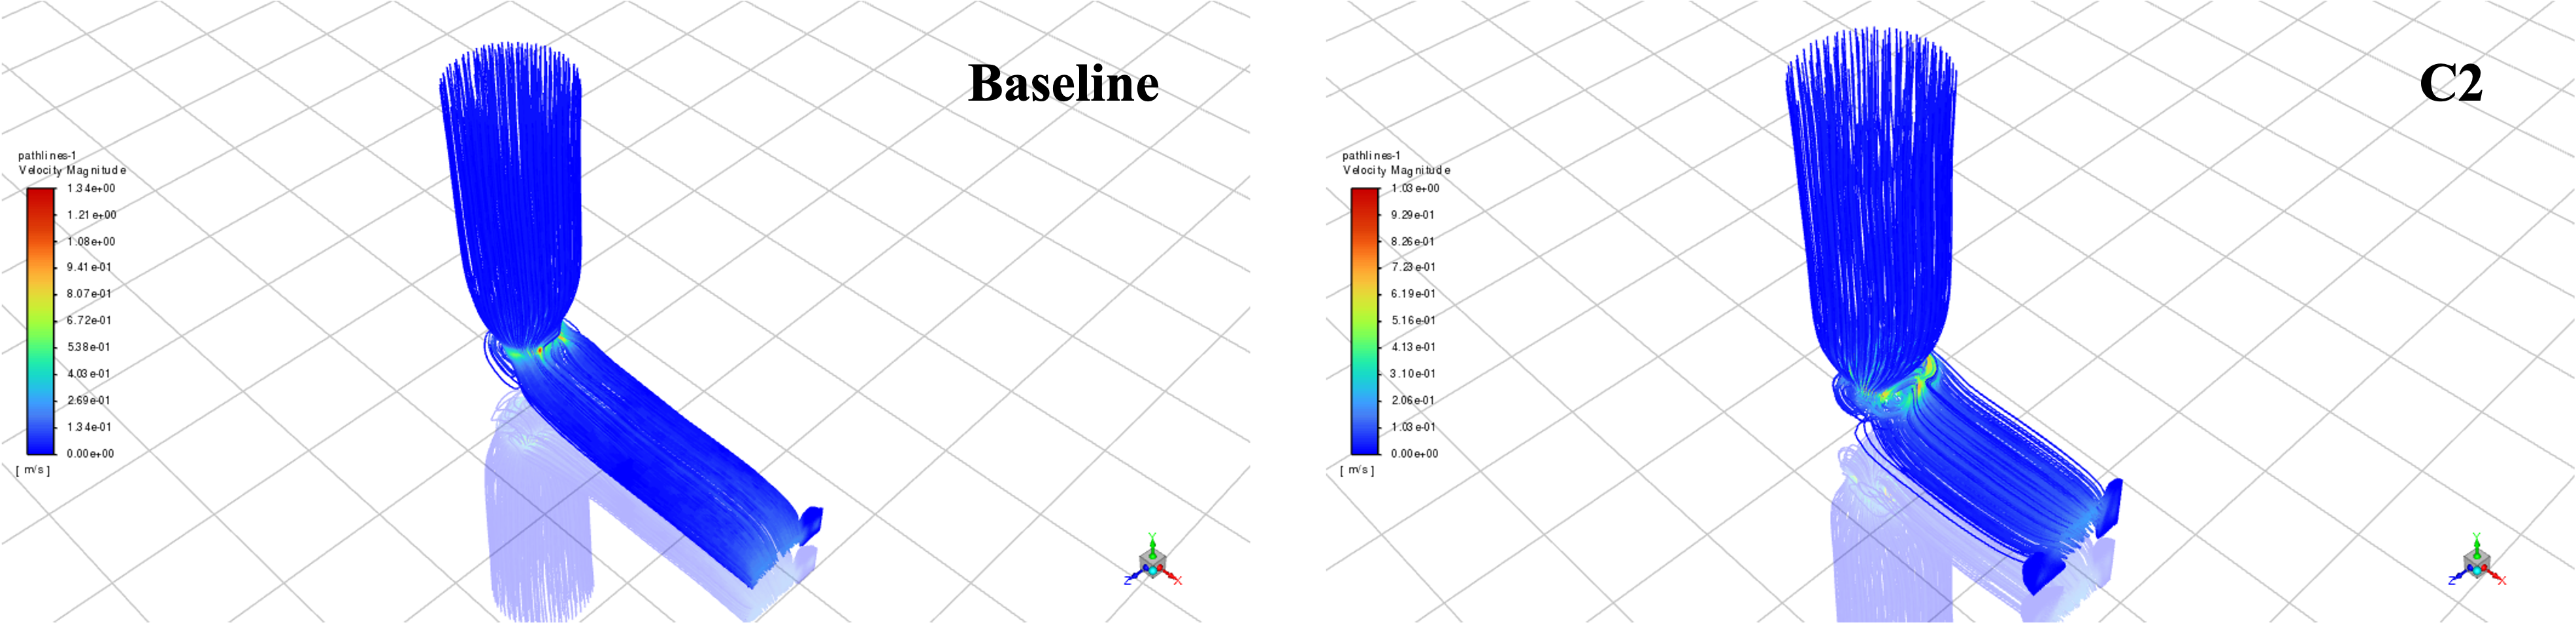
\includegraphics[width=0.9\textwidth]{figures/4.15.png}
  \caption{C2与基线工况的速度流线对比}
  \label{fig:4.15}
\end{figure}

\cref{fig:4.15}将C2与Baseline的速度场进行了对比。在Baseline工况中，顶板的存在对浆体形成封闭约束，使流体无法向上方逸散，所有动能被强制导向基底方向，形成有效的接触压力；而在C2工况中，去除顶板后流体可向上方自由扩散，约束空间开放，浆体的大部分动能以扩散流动的形式耗散，无法有效转化为对基底面的静压力，导致接触压力大幅降低。

C2工况还呈现出一个值得关注的特殊现象：整形转向后出口处的面积加权平均压力（8563~Pa）高于喷嘴平面处（3562~Pa），表现出沿流动方向的非单调压力分布特征。该现象的产生可能与C2工况下流场结构的显著变化密切相关。在去除顶板后，出口区域失去了原有的上壁约束，浆体在离开喷嘴后发生明显的自由扩散。由于流体向两侧扩张，出口截面附近局部区域出现低速滞留甚至回流现象，并伴随局部低压区形成，最小静压达到$-302$~Pa。这些低压区域在面积加权平均过程中显著拉低了喷嘴平面处的平均压力值。相比之下，整形转向后真实出口区域仍受到前挡板的局部约束作用，流体横向扩散受到抑制，局部流体减速并产生一定程度的压力积聚，因此其面积加权平均压力反而高于喷嘴平面处。这个结果并不违反流体力学规律，而是无顶板工况下自由扩散、局部回流以及约束条件变化共同作用的结果。这也说明，在存在明显流场分离与扩散结构的工况下，传统基于截面平均压力的比较方法需要结合具体流场形态进行综合分析。

C2工况的分析证明：整形板顶板是产生有效基底接触压力的核心结构，其封闭约束作用不可或缺。在实际打印系统设计中，整形板顶板的存在是提升层间粘结性能的必要条件。

\subsection{拓扑几何优化分析（C3工况）}

C3工况在C1-3几何参数（$TL = 60$~mm，$\theta = 60°$，$L = 20$~mm，$\alpha = 15°$）基础上，对喷嘴收缩段与直管段的转角处、整形板各转角处进行3-5~mm的圆角过渡处理（Fillet），以探究几何倒角对流场特性的影响。\cref{tab:4.8}总结了C3工况与基础工况的重点研究指标结果对比。

\begin{table}[!htb]
  \centering
  \caption{C3工况评价指标对比表}\label{tab:4.8}
  \renewcommand{\arraystretch}{1.3}
  \begin{tabular}{lcccccccc}
    \toprule
    \textbf{工况} & $TL$ & $\theta$ & $L$ & $\alpha$ & $P_{sub}$(Pa) & $WSS_{nozzle}$ & $\eta_p$ & $UI$ \\
    \midrule
    Baseline & 50 & 30 & 20 & 10 & 8310  & 84.9  & 0.421 & 1.78 \\
    C3       & 60 & 60 & 20 & 15 & 21702 & 25.13 & 0.560 & 1.58 \\
    \bottomrule
  \end{tabular}
\end{table}

压力结果方面，C3的$P_{sub,AWA} = 21702$~Pa，与C1-3的21677~Pa相差不足0.1\%，差异可忽略。这一结果说明，转角处的几何倒角对整体压力场的宏观分布影响极为有限。这说明基底接触压力主要由流道的宏观收缩比（由$\theta$决定）和整形板的楔形约束几何（由$\alpha$和$TL$决定）所主导，局部转角的圆化处理不改变这两个主控因素，因此对压力场的影响在工程精度范围内可视为零。

然而，剪切应力结果却呈现出显著的差异：C3的$WSS_{nozzle} = 25.1$~Pa，较C1-3的41.1~Pa降低了39\%。倒角消除了收缩段与直管段转角处的几何尖角，流线在此区域得以平滑过渡，避免了尖角处流动分离导致的局部高速梯度集中，在流场上表现为高剪切速率区被显著抑制，近壁速度梯度分布更为均匀，因而壁面剪切应力大幅降低。

综合而言，C3工况以几乎不损失接触压力性能（$\Delta P_{sub} < 0.1\%$）为代价，实现了$WSS_{nozzle}$ 39\%的显著改善，是本课题研究工况中最佳的几何构型。倒角设计作为一种低成本的几何优化手段，在实际打印喷嘴制造中值得推广应用。

\cref{fig:4.16}总结了C3工况的完整流场速度、压力、壁面剪切应力展示图；\cref{fig:4.17}展示了C3与Baseline工况五项指标归一化后的雷达图对比，直观展示了C3在各维度的综合优越性。

\begin{figure}[!htb]
  \centering
  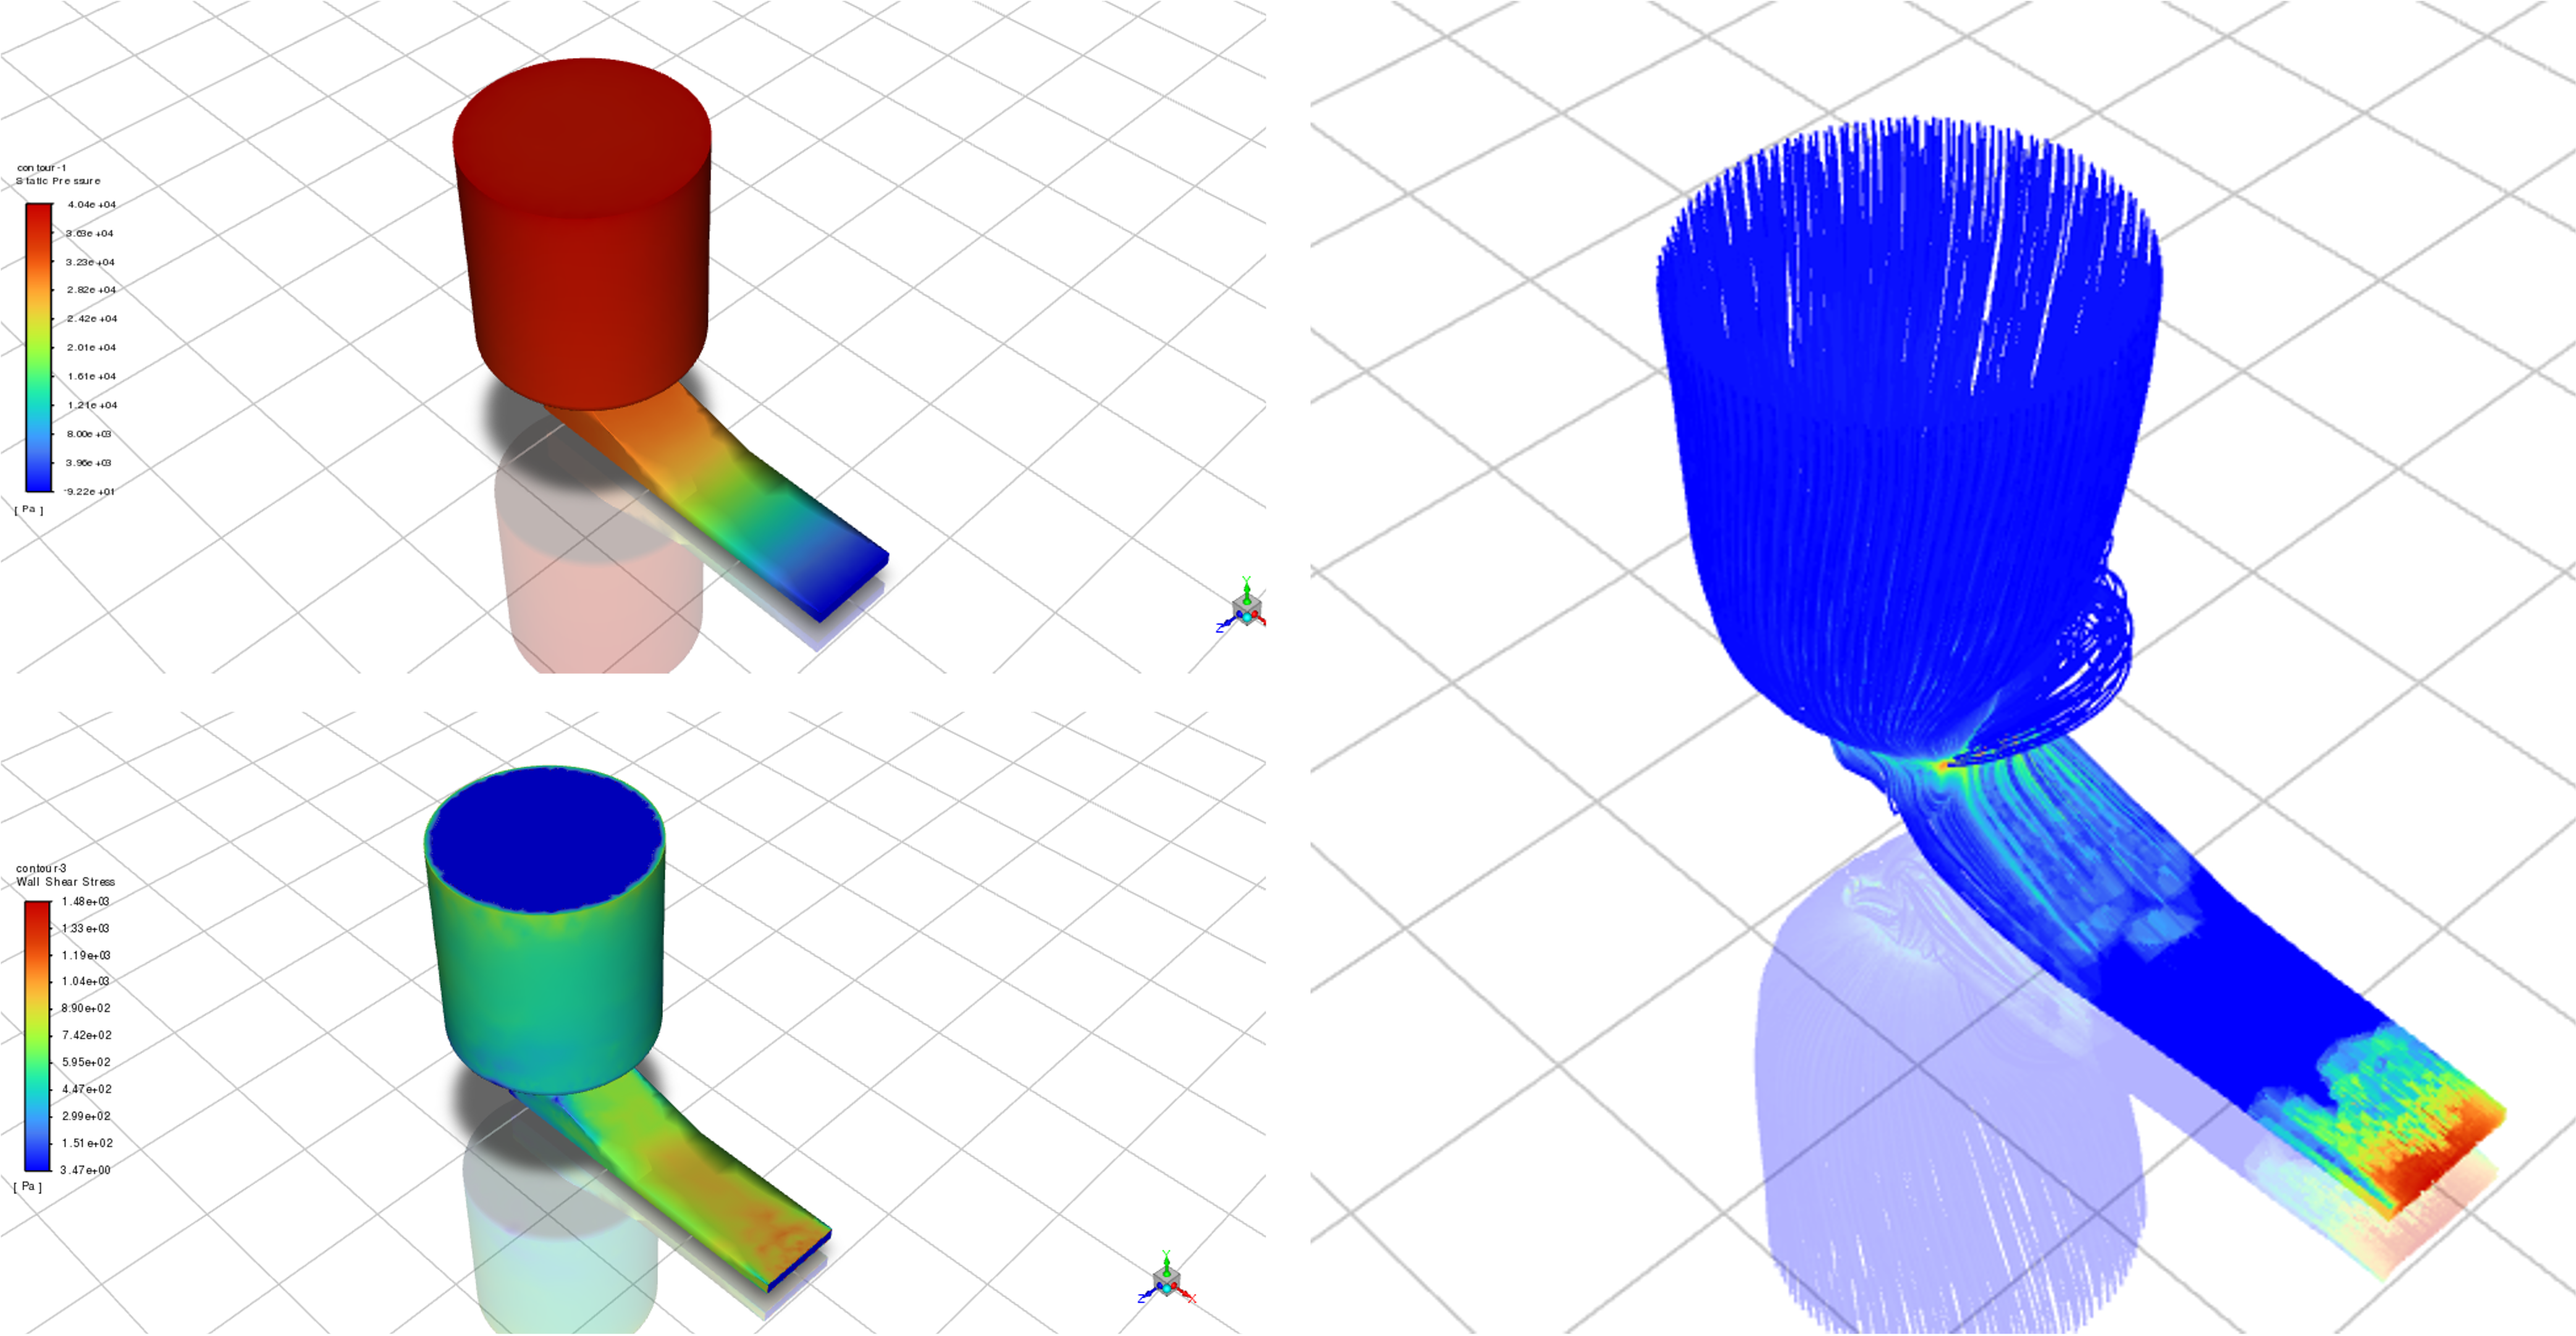
\includegraphics[width=0.9\textwidth]{figures/4.16.png}
  \caption{C3工况流场速度、压力、壁面剪切应力图}
  \label{fig:4.16}
\end{figure}

\begin{figure}[!htb]
  \centering
  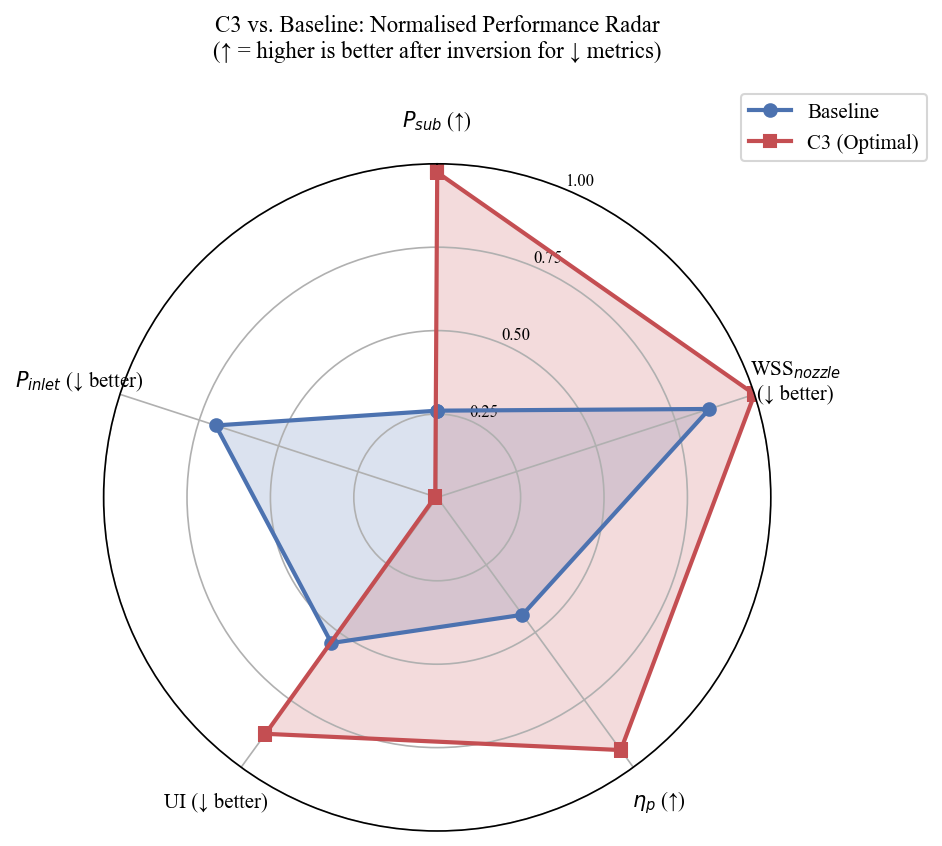
\includegraphics[width=0.7\textwidth]{figures/4.17.png}
  \caption{C3工况与基线工况对比雷达图}
  \label{fig:4.17}
\end{figure}

\section{参数影响规律综合对比}

\subsection{代表性工况数据汇总表}

\cref{tab:4.9}列举了代表性工况的完整评价指标。从对照工况C2（无顶板，$P_{sub} = 3436$~Pa）到最优工况C3（$P_{sub} = 21702$~Pa），基底接触压力跨越了约6倍的范围，说明喷嘴与整形板的几何设计对打印层间粘结性能具有决定性影响，远超材料流变参数微调所能带来的效益。

\begin{table}[!htb]
  \centering
  \caption{代表性工况评价指标汇总表}\label{tab:4.9}
  \renewcommand{\arraystretch}{1.3}
  \footnotesize
  \begin{tabular}{lcccccccccc}
    \toprule
    \textbf{工况} & $\theta$ & $L$ & $TL$ & $\alpha$ & $P_{sub,AWA}$ & $P_{sub,Max}$ & $WSS_{nozzle}$ & $\eta_p$ & $UI$ \\
    \midrule
    Baseline & 30° & 20 & 50 & 10° & 8310  & 13983 & 84.9  & 0.421 & 1.776 \\
    A1-4     & 60° & 20 & 50 & 10° & 9926  & 17858 & 35.0  & 0.447 & 1.842 \\
    B1-3     & 30° & 20 & 50 & 15° & 12081 & 19501 & 77.1  & 0.481 & 1.645 \\
    B2-4     & 30° & 20 & 70 & 10° & 12833 & 21089 & 102.1 & 0.483 & 1.683 \\
    C2       & 30° & 20 & 0  & 10° & 3436  & 6238  & 382.2 & 0.300 & 2.087 \\
    C3       & 60° & 20 & 60 & 15° & 21702 & 34234 & 25.1  & 0.560 & 1.582 \\
    \bottomrule
  \end{tabular}
\end{table}

\subsection{各参数影响幅度定量对比}

基于各研究线的单因素极差分析，四个设计变量对$P_{sub,AWA}$的影响幅度排序为：
\begin{equation}\label{eq:rank}
  \alpha\ (198\%) > TL\ (82.9\%) \gg \theta\ (19.7\%) > L\ (12.8\%).
\end{equation}

\begin{figure}[!htb]
  \centering
  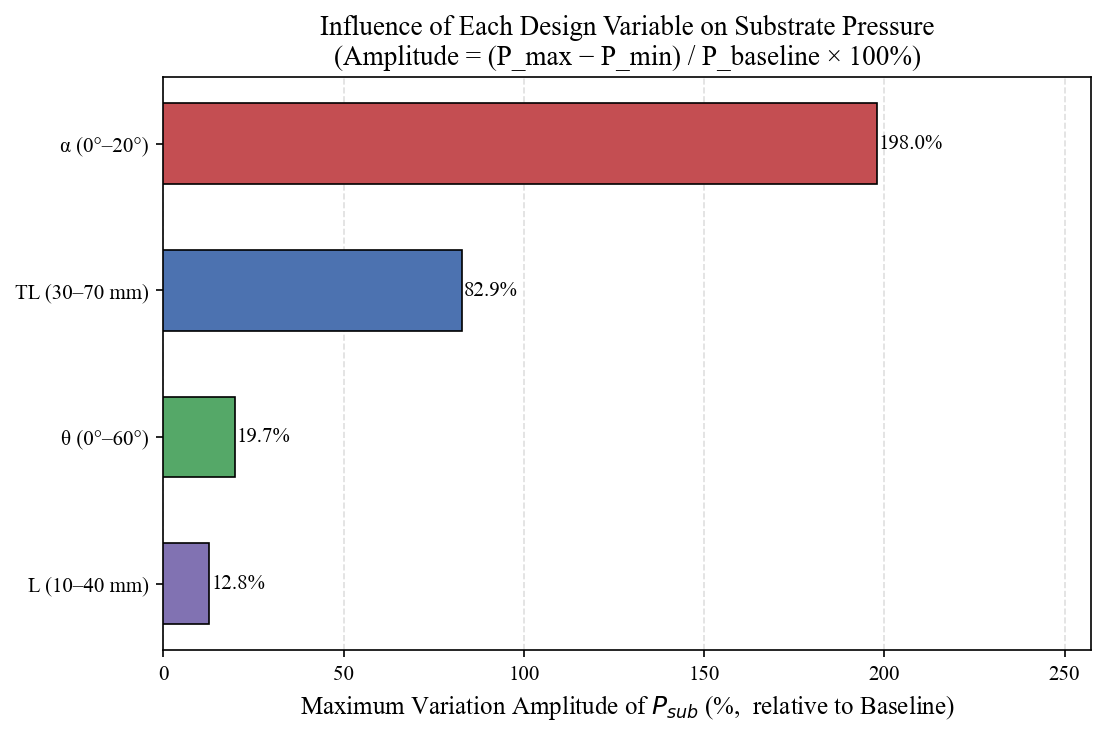
\includegraphics[width=0.75\textwidth]{figures/4.18.png}
  \caption{各参数对基底接触压力影响幅度对比柱状图}
  \label{fig:4.18}
\end{figure}

\cref{fig:4.18}以柱状图形式直观呈现了这一排序。$\alpha$的影响幅度远超其他变量，是调控基底接触压力最敏感的手段，但同时受到层高约束的强烈制约；$TL$以中等敏感性和充足的层高余量成为最具工程实用性的调控参数；$\theta$的影响幅度虽相对有限，但其兼具降低壁面剪切应力特性，具有独特工程价值；$L$的影响幅度最小且统计不显著，在工程设计中可视为次要参数。这一影响幅度排序为多目标优化提供了关键的先验信息，有助于理解NSGA-II优化结果中各参数趋向边界值的内在逻辑。

\subsection{Pearson相关分析}

为从统计学角度定量验证上述定性分析结论，对全部20个工况的四个设计变量与五项评价指标进行Pearson线性相关分析，结果如\cref{fig:4.19}、\cref{fig:4.20}所示。

\begin{figure}[!htb]
  \centering
  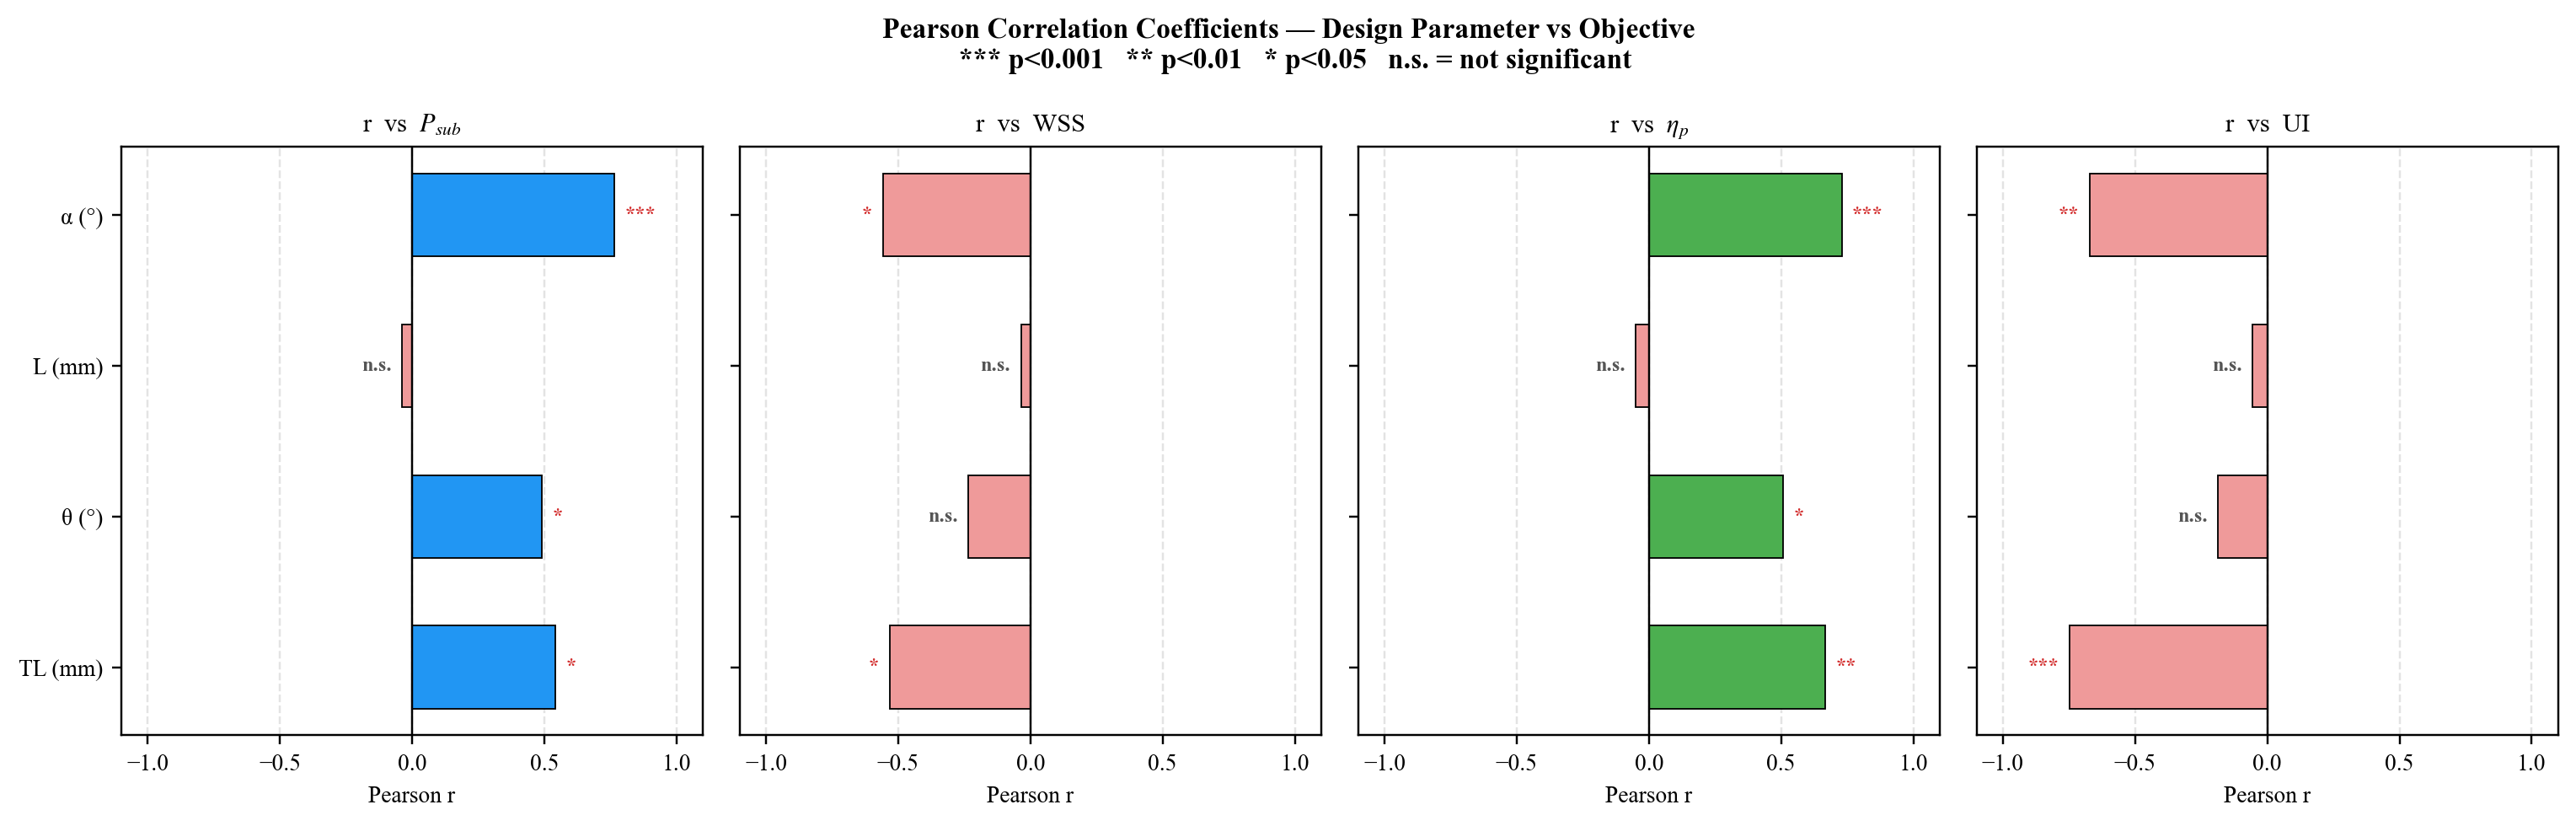
\includegraphics[width=0.8\textwidth]{figures/4.19.png}
  \caption{敏感性分析柱状图（前四项评价指标）}
  \label{fig:4.19}
\end{figure}

\begin{figure}[!htb]
  \centering
  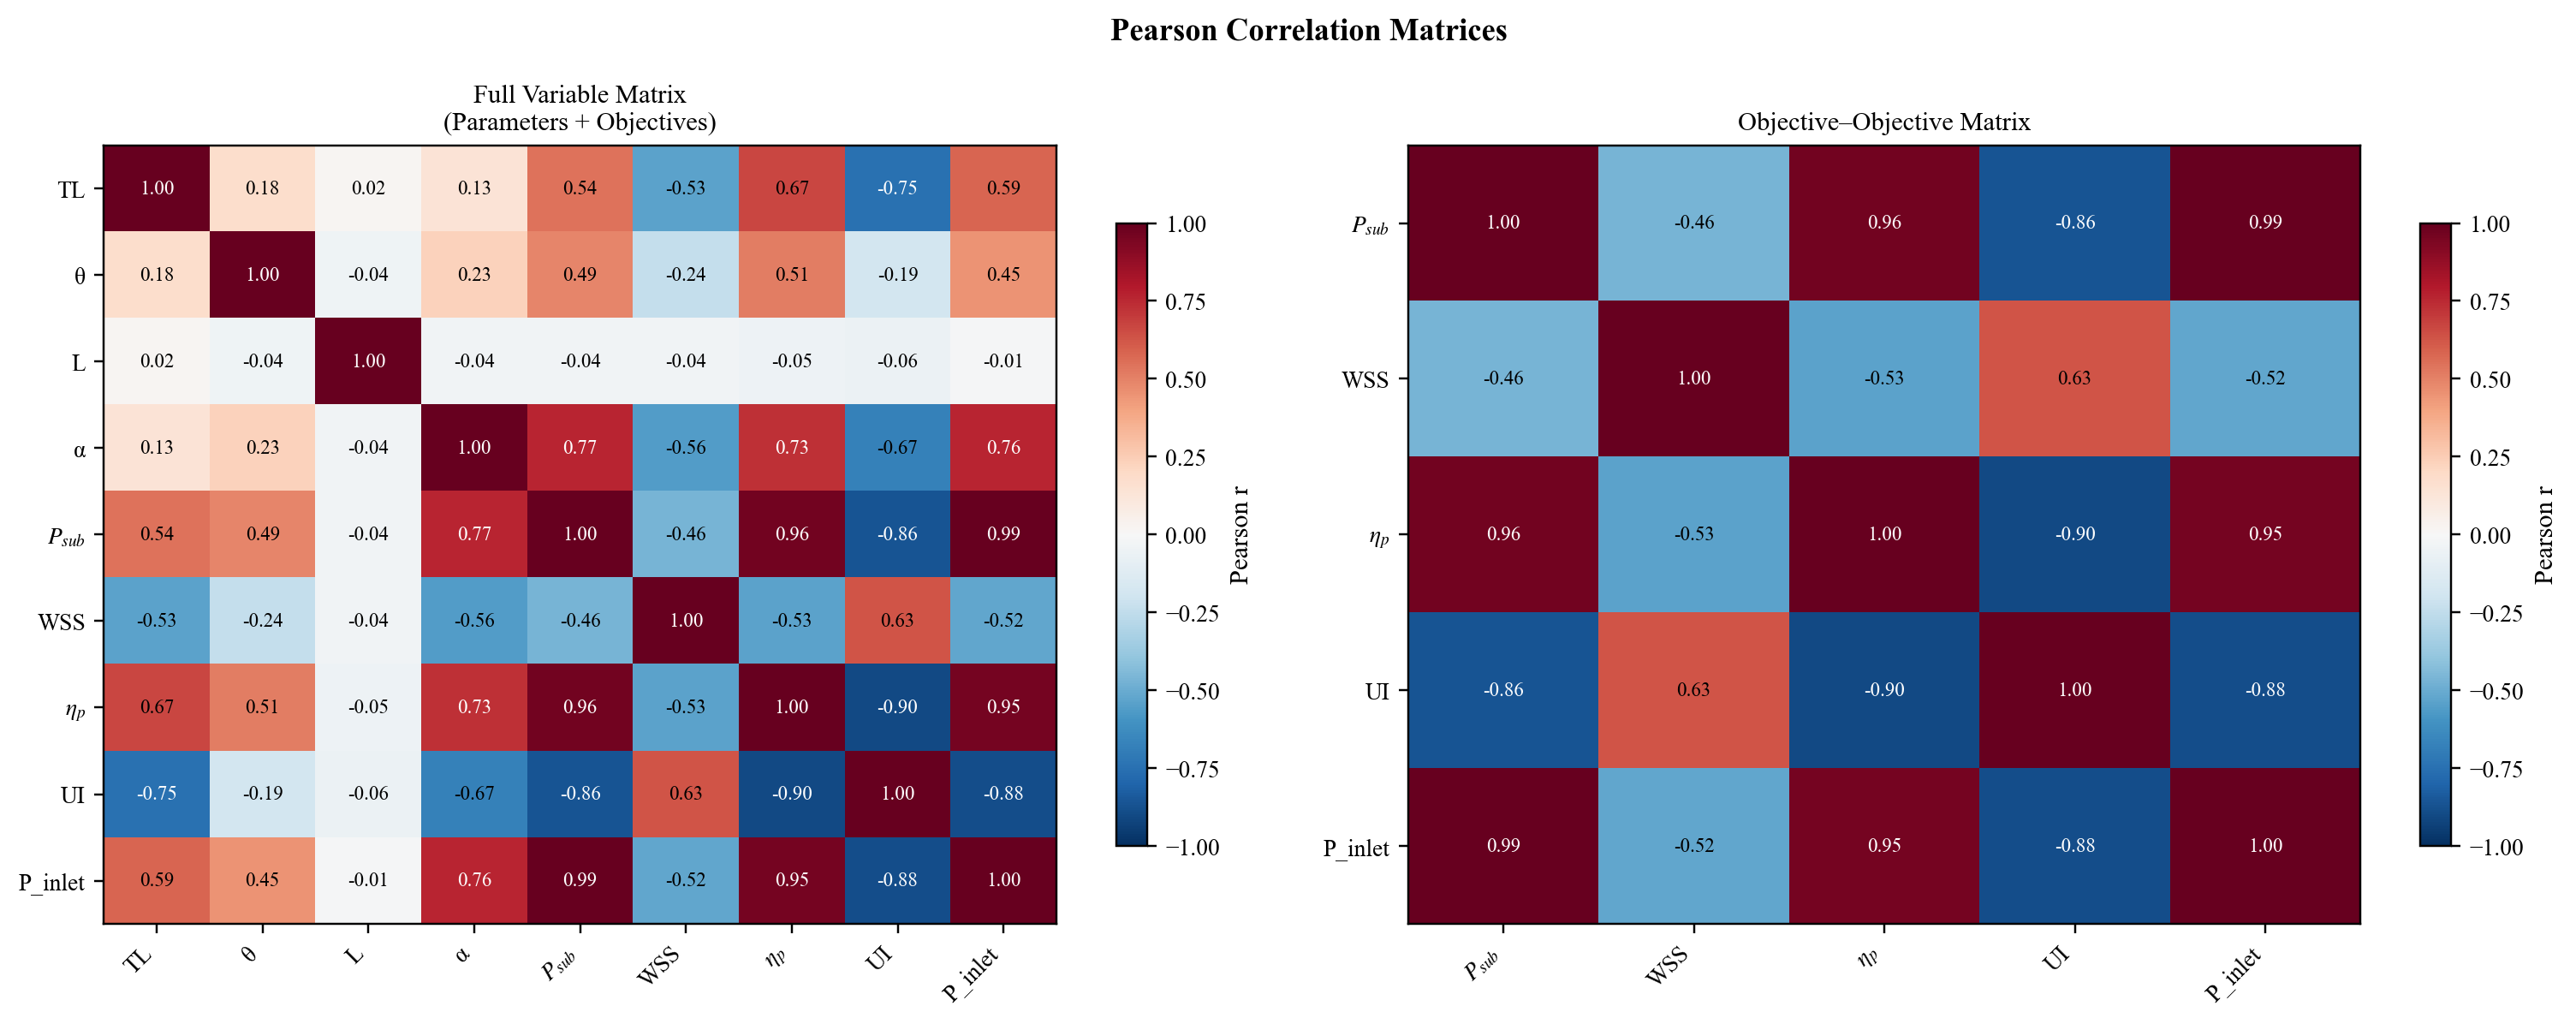
\includegraphics[width=0.95\textwidth]{figures/4.20.png}
  \caption{参数-目标全变量相关性热力图（左）、目标-目标相关性热力图（右）}
  \label{fig:4.20}
\end{figure}

对于核心指标$P_{sub,AWA}$，各变量的相关系数及显著性如\cref{tab:4.10}所示。这一结果与单因素极差分析的排序高度吻合，在统计层面上进一步证实了$\alpha$和$TL$是影响基底接触压力的显著参数，而$L$的影响在统计意义上可视为零，不宜作为主动调控手段。

\begin{table}[!htb]
  \centering
  \caption{$P_{sub,AWA}$相关系数与显著性汇总表}\label{tab:4.10}
  \renewcommand{\arraystretch}{1.3}
  \begin{tabular}{lcccc}
    \toprule
    \textbf{指标} & \textbf{Pearson r} & \textbf{Spearman r} & \textbf{P-value} & \textbf{Significance} \\
    \midrule
    $TL$       & $+0.541$ & $+0.746$ & 0.0137 & * \\
    $\theta$   & $+0.490$ & $+0.420$ & 0.0285 & * \\
    $L$        & $-0.038$ & $+0.080$ & 0.8726 & n.s. \\
    $\alpha$   & $+0.765$ & $+0.794$ & 0.0001 & *** \\
    \bottomrule
  \end{tabular}
\end{table}

目标-目标相关性热力图揭示了另一个具有工程意义的发现：$P_{inlet}$与$P_{sub,AWA}$之间的Pearson相关系数高达$r = 0.994$（$p < 0.001$），两者之间存在近乎完美的线性共线关系。这意味着在本研究的喷嘴-整形板系统中，提升基底接触压力与增大泵送入口压力是几乎等价的操作，两者无法独立解耦。

\chapter{多目标Pareto优化分析}\label{chap:optimization}

参数化研究揭示了四个几何变量对各评价指标的单因素影响规律。然而，工程设计问题的本质是多目标权衡：同时追求高基底接触压力、低剪切应力、高压力传递效率与低泵送能耗，这些目标之间往往存在相互制约关系，无法通过单一参数调整同时满足所有需求。识别工程问题中需要完成的目标并将其按照紧迫性进行排序，最终通过多目标分析体系寻找一个满足多个要求的最优解，才能在实际的工程问题中找到一个权衡利弊的答案。为此，本章构建多目标Pareto优化分析框架，系统识别各目标之间的权衡关系，确定可行参数空间内的最优设计方案。

\section{多目标优化框架}

\subsection{设计变量与约束条件}

本研究的优化设计变量为四个几何参数，构成设计向量：
\begin{equation}\label{eq:design-vector}
  \mathbf{x} = (TL, \theta, L, \alpha) \in [30, 70] \times [15°, 60°] \times [10, 40] \times [0°, 20°].
\end{equation}
各变量的物理含义与取值范围见\cref{tab:5.1}。

\begin{table}[!htb]
  \centering
  \caption{设计变量定义与约束汇总表}\label{tab:5.1}
  \renewcommand{\arraystretch}{1.3}
  \begin{tabular}{cllll}
    \toprule
    \textbf{变量} & \textbf{物理含义} & \textbf{下界} & \textbf{上界} & \textbf{单位} \\
    \midrule
    $TL$     & 整形板长度    & 30 & 70           & mm \\
    $\theta$ & 喷嘴收缩角    & 15 & 60           & ° \\
    $L$      & 喷嘴竖直高度  & 10 & 40           & mm \\
    $\alpha$ & 整形板倾斜角  & 0  & 20（受$H$约束） & ° \\
    \bottomrule
  \end{tabular}
\end{table}

优化问题受到以下几何可行性约束的限制。整形板出口处的层高$H$由\cref{chap:parametric}第\ref{sec:alpha-influence}节推导的解析关系决定，其需满足：
\begin{equation}\label{eq:H-constraint}
  5~\text{mm} \leq H = Z_0 - TL \cdot \sin(\alpha) \leq 20~\text{mm},
\end{equation}
其中下界$H_{min} = 5$~mm保证沉积层具有最小可行厚度，上界$H_{max} = 20$~mm对应整形板完全水平（$\alpha = 0°$）时的层高上限。该约束本质上是对$\alpha$的上界施加了依赖于$TL$的动态限制。在最严苛情况下（$TL = 70$~mm），$\alpha$的解析上界为：
\begin{equation}\label{eq:alpha-max-strict}
  \alpha_{max} = \arcsin\left( \frac{Z_0 - H_{min}}{TL_{max}} \right) = \arcsin\left( \frac{22 - 5}{70} \right) = 14.06°.
\end{equation}
\cref{fig:5.1}在$\alpha$-$TL$参数平面内直观展示了几何可行域的边界。可以看出，随$TL$增大，可行的$\alpha$上界单调降低，呈现出整形板长度与倾斜角之间的固有几何耦合关系。图中同时标注了全部CFD工况点的位置，其中位于红色不可行区的B1-4工况（$\alpha = 20°$，$TL = 50$~mm，$H = 4.90$~mm）被排除出优化可行域。

\begin{figure}[!htb]
  \centering
  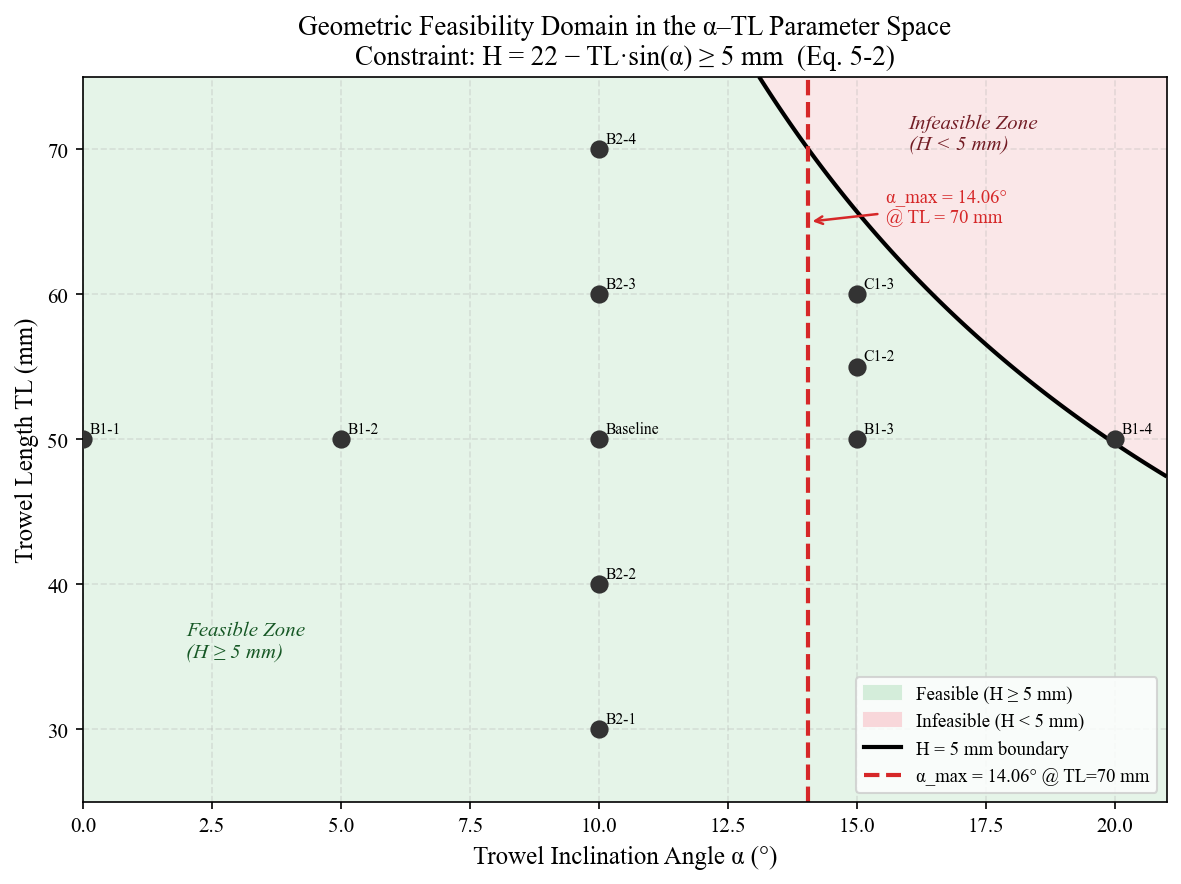
\includegraphics[width=0.8\textwidth]{figures/5.1.png}
  \caption{几何可行域示意图（$\alpha$-$TL$参数平面）}
  \label{fig:5.1}
\end{figure}

\subsection{五目标优化问题定义}

本研究将优化问题统一表述为最小化问题。对于原本需要最大化的目标，通过取负值将其转化为最小化形式。

本课题主要研究了两个优化问题。四目标优化平衡了基底面压力、喷嘴出口截面壁面剪切应力、压力传递效应与压力非均匀性指数，是在已有数据集的基础上进行目标简化，与此同时权衡重要性能、经济指标的结果。四目标优化问题的数学表述为：
\begin{equation}\label{eq:4-obj}
  \min_{\mathbf{x}} F(\mathbf{x}) = (-P_{sub,AWA},\ WSS_{nozzle},\ -\eta_p,\ UI).
\end{equation}

五目标优化是对四目标框架的重要扩展，将作为泵送能耗的代理指标$P_{inlet}$纳入其中。过高的泵送压力不仅增加能耗，还对泵送设备的密封性和使用寿命提出更高要求。在四目标框架中，$P_{inlet}$未被显式约束，优化器可能给出需要极高泵送压力的方案；纳入第五目标后，优化框架能够明确量化为获得更高接触压力所需付出的泵送代价，从而为工程决策提供更完整的信息。五目标优化问题的数学表述为：
\begin{equation}\label{eq:5-obj}
  \min_{\mathbf{x}} G(\mathbf{x}) = (-P_{sub,AWA},\ WSS_{nozzle},\ -\eta_p,\ UI,\ P_{inlet}).
\end{equation}

各目标的物理定义、优化方向及工程意义总结在\cref{tab:5.2}中。

\begin{table}[!htb]
  \centering
  \caption{优化目标定义、方向与工程意义汇总表}\label{tab:5.2}
  \renewcommand{\arraystretch}{1.3}
  \begin{tabular}{lllll}
    \toprule
    \textbf{目标} & \textbf{定义} & \textbf{方向} & \textbf{内化方向} & \textbf{工程意义} \\
    \midrule
    $f_1 = -P_{sub,AWA}$ & 基底接触压力     & 最大化 & 最小化 & 层间粘结强度 \\
    $f_2 = WSS_{nozzle}$ & 喷嘴剪切应力     & 最小化 & 最小化 & 材料损伤与磨损 \\
    $f_3 = -\eta_p$      & 压力传递效率     & 最大化 & 最小化 & 泵送经济性 \\
    $f_4 = UI$           & 压力非均匀性     & 最小化 & 最小化 & 层间质量均匀性 \\
    $f_5 = P_{inlet}$    & 入口压力         & 最小化 & 最小化 & 泵送能耗代理 \\
    \bottomrule
  \end{tabular}
\end{table}

\section{代理模型建立}

遗传算法需要在优化过程中需要对目标函数进行数万次评估，而三维几何建模与CFD分析需要很大的计算能力与时间，这让代理直接调用CFD仿真在计算成本上基本不可行。本课题于是建立了一个能够快速预测目标函数值的代理模型（Surrogate Model），以完成后续分析。

\subsection{多项式RSM（2阶Ridge回归）}

选用2阶多项式响应面方法（Response Surface Methodology，RSM）配合Ridge正则化（正则化系数$\lambda = 1.0$）作为代理模型。2阶多项式RSM的基函数展开形式为：
\begin{equation}\label{eq:rsm}
  \hat{f}(\mathbf{x}) = \beta_0 + \sum_i \beta_i x_i + \sum_i \beta_{ii} x_i^2 + \sum_{i<j} \beta_{ij} x_i x_j.
\end{equation}
对于4个设计变量，该模型共包含：4个线性项、4个二次项、6个交叉项，1个截距项，共计15个系数。考虑到本研究可用的可行工况数量为17个，2阶多项式RSM与数据规模匹配较好，在保证拟合能力的同时不至于严重过拟合。

在模型选择方面，本课题同时评估了高斯过程回归（Gaussian Process Regression，GPR）和梯度提升回归（Gradient Boosting Regression，GBR）方法。GPR在理论上具有较强的非线性拟合能力，但在仅17个数据点的条件下，其留一法交叉验证（LOO-CV）得到的$R^2$仅为0.37，泛化能力不稳定；GBR属于集成学习方法，对小样本同样容易出现过拟合。相比之下，2阶多项式RSM配合Ridge正则化在小样本工程参数优化中具有更稳定的泛化表现，且系数具有明确的物理解释性（各变量的线性项、二次项系数直接反映其对目标函数的影响方向与强度），因此选用该方法作为本研究的代理模型。

\subsection{留一法交叉验证（LOO-CV）}

为客观评估代理模型的预测精度，采用留一法交叉验证（Leave-One-Out Cross-Validation，LOO-CV）对各目标的代理模型进行验证。LOO-CV能够在不额外消耗CFD计算资源的前提下，对小样本代理模型的泛化能力给出无偏估计。五目标代理模型的LOO-CV结果汇总于\cref{tab:5.3}，对应的预测值与实际值散点图见\cref{fig:5.2}。预测模型的集成多项式RSM响应面如\cref{fig:5.3}所示。

\begin{figure}[!htb]
  \centering
  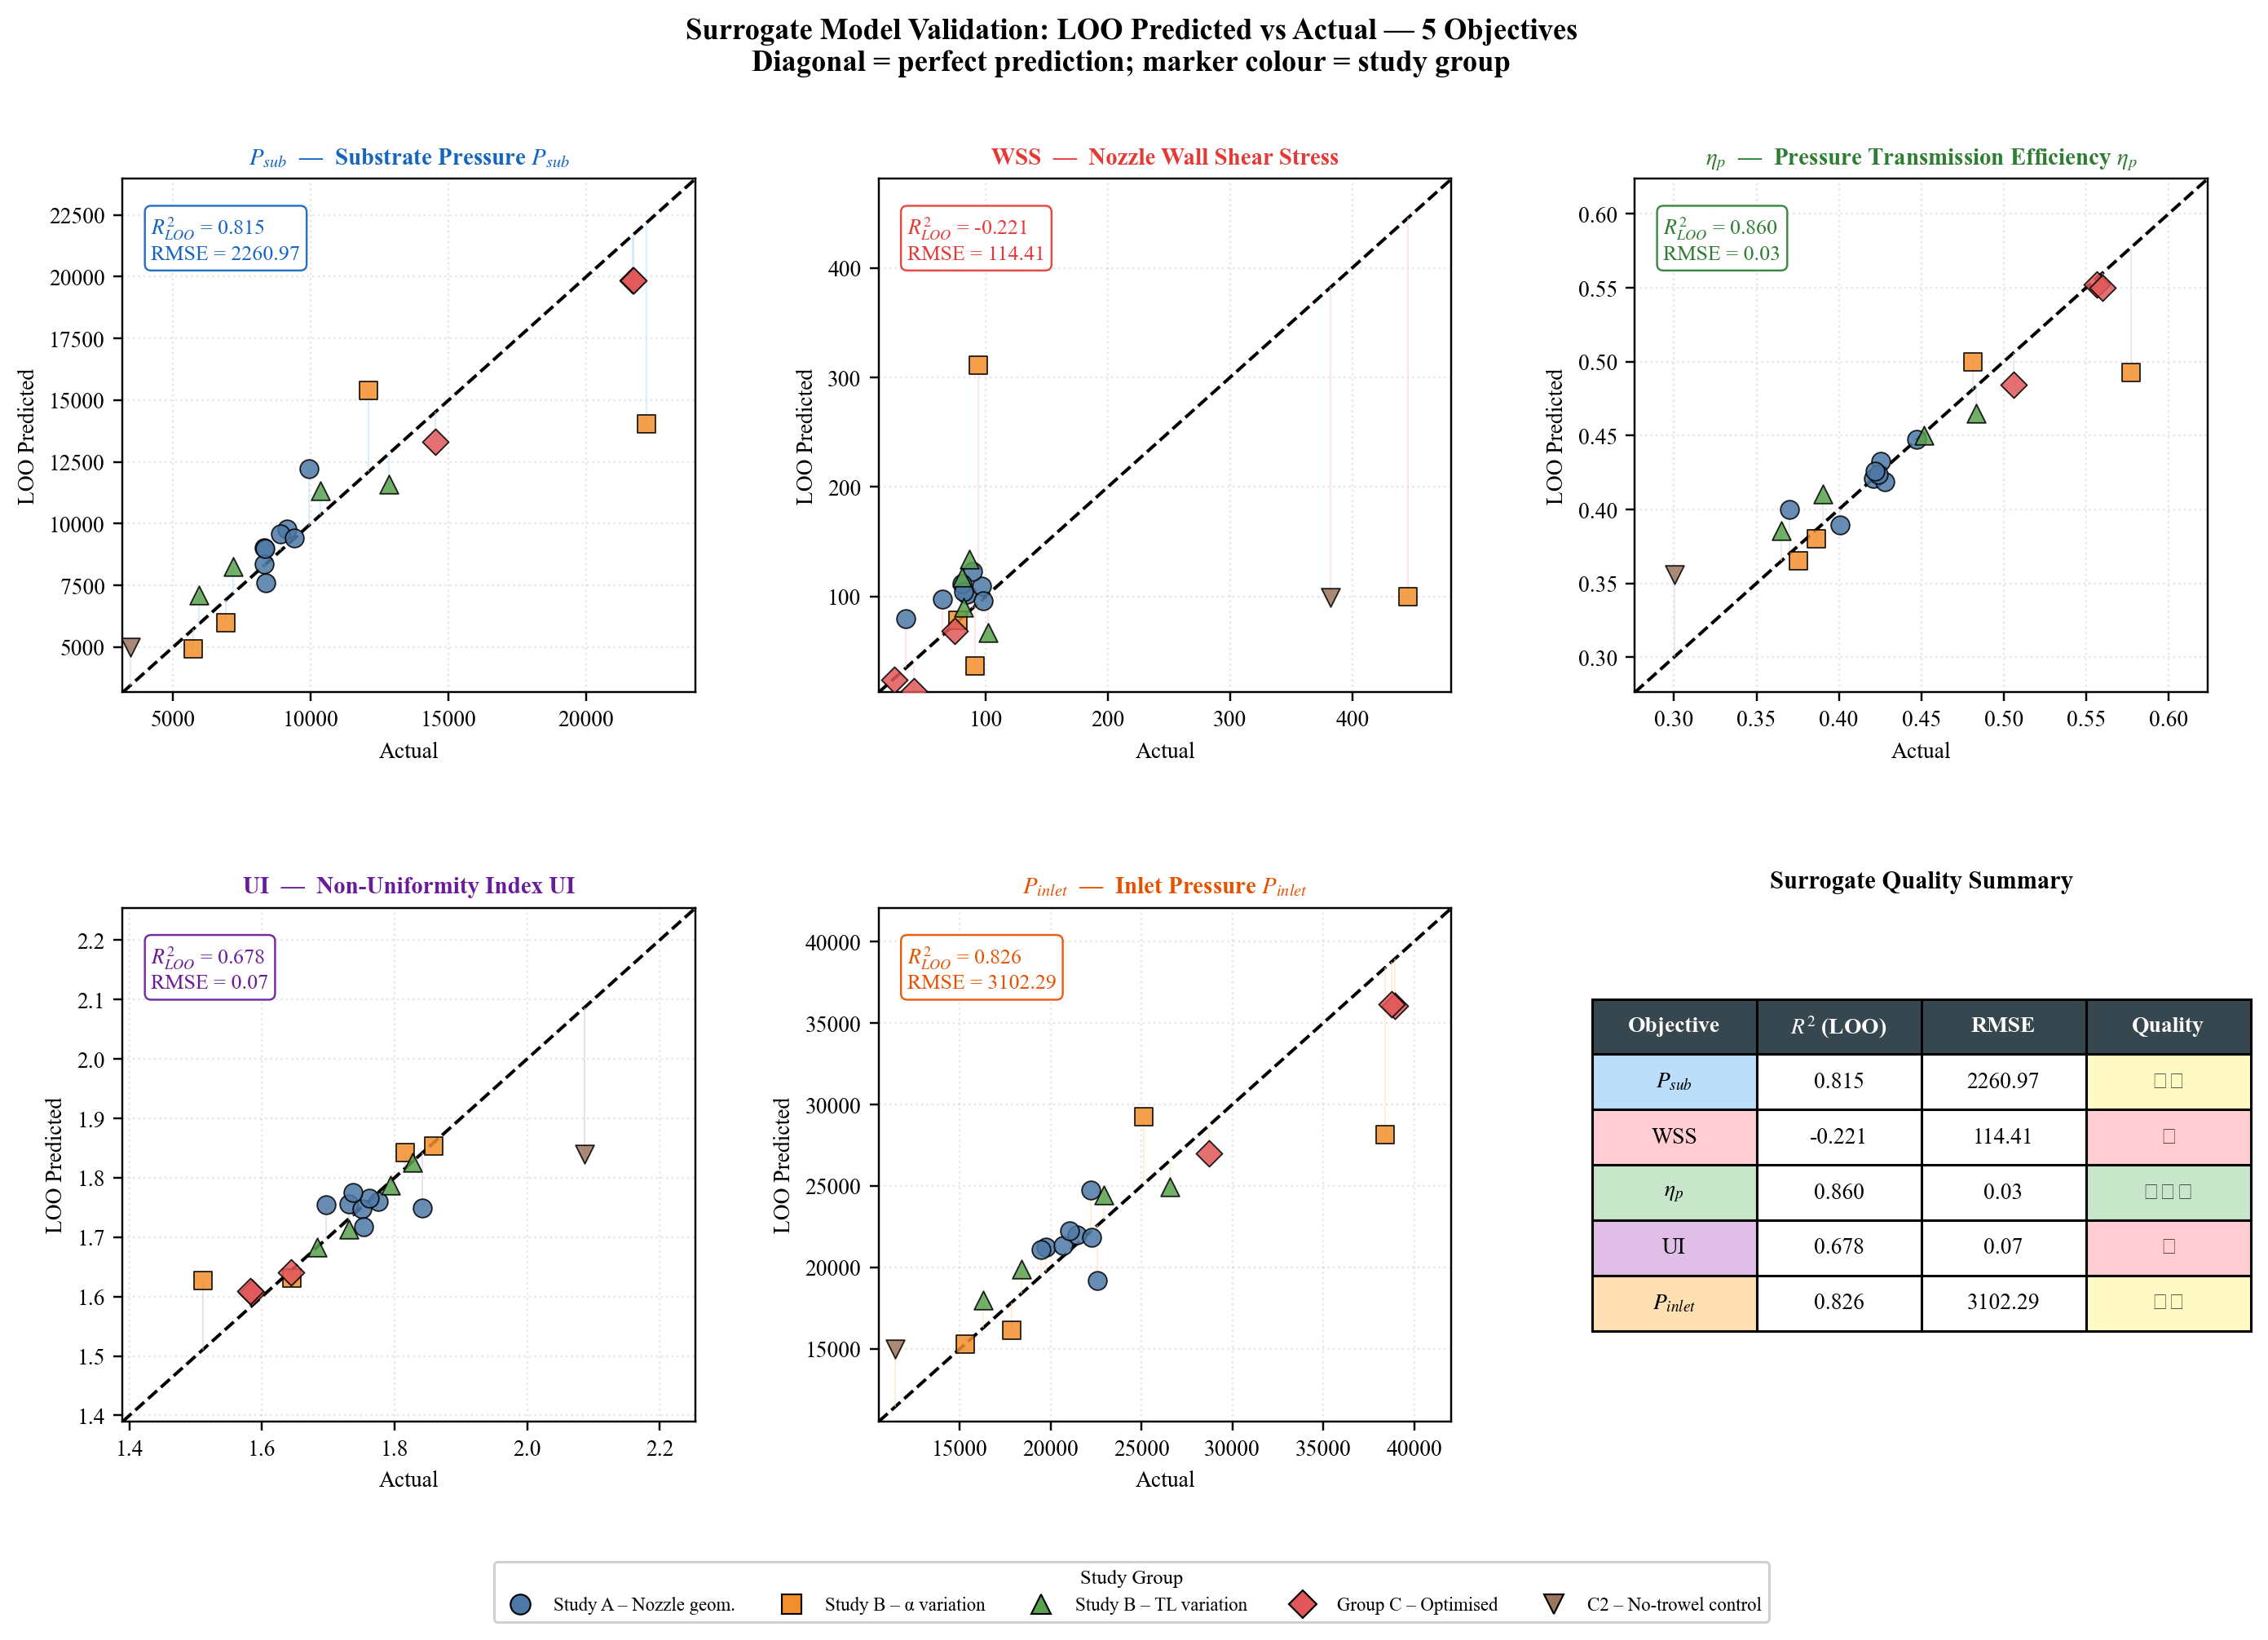
\includegraphics[width=0.9\textwidth]{figures/5.2.png}
  \caption{各目标LOO预测值与实际值对比散点图}
  \label{fig:5.2}
\end{figure}

\begin{figure}[!htb]
  \centering
  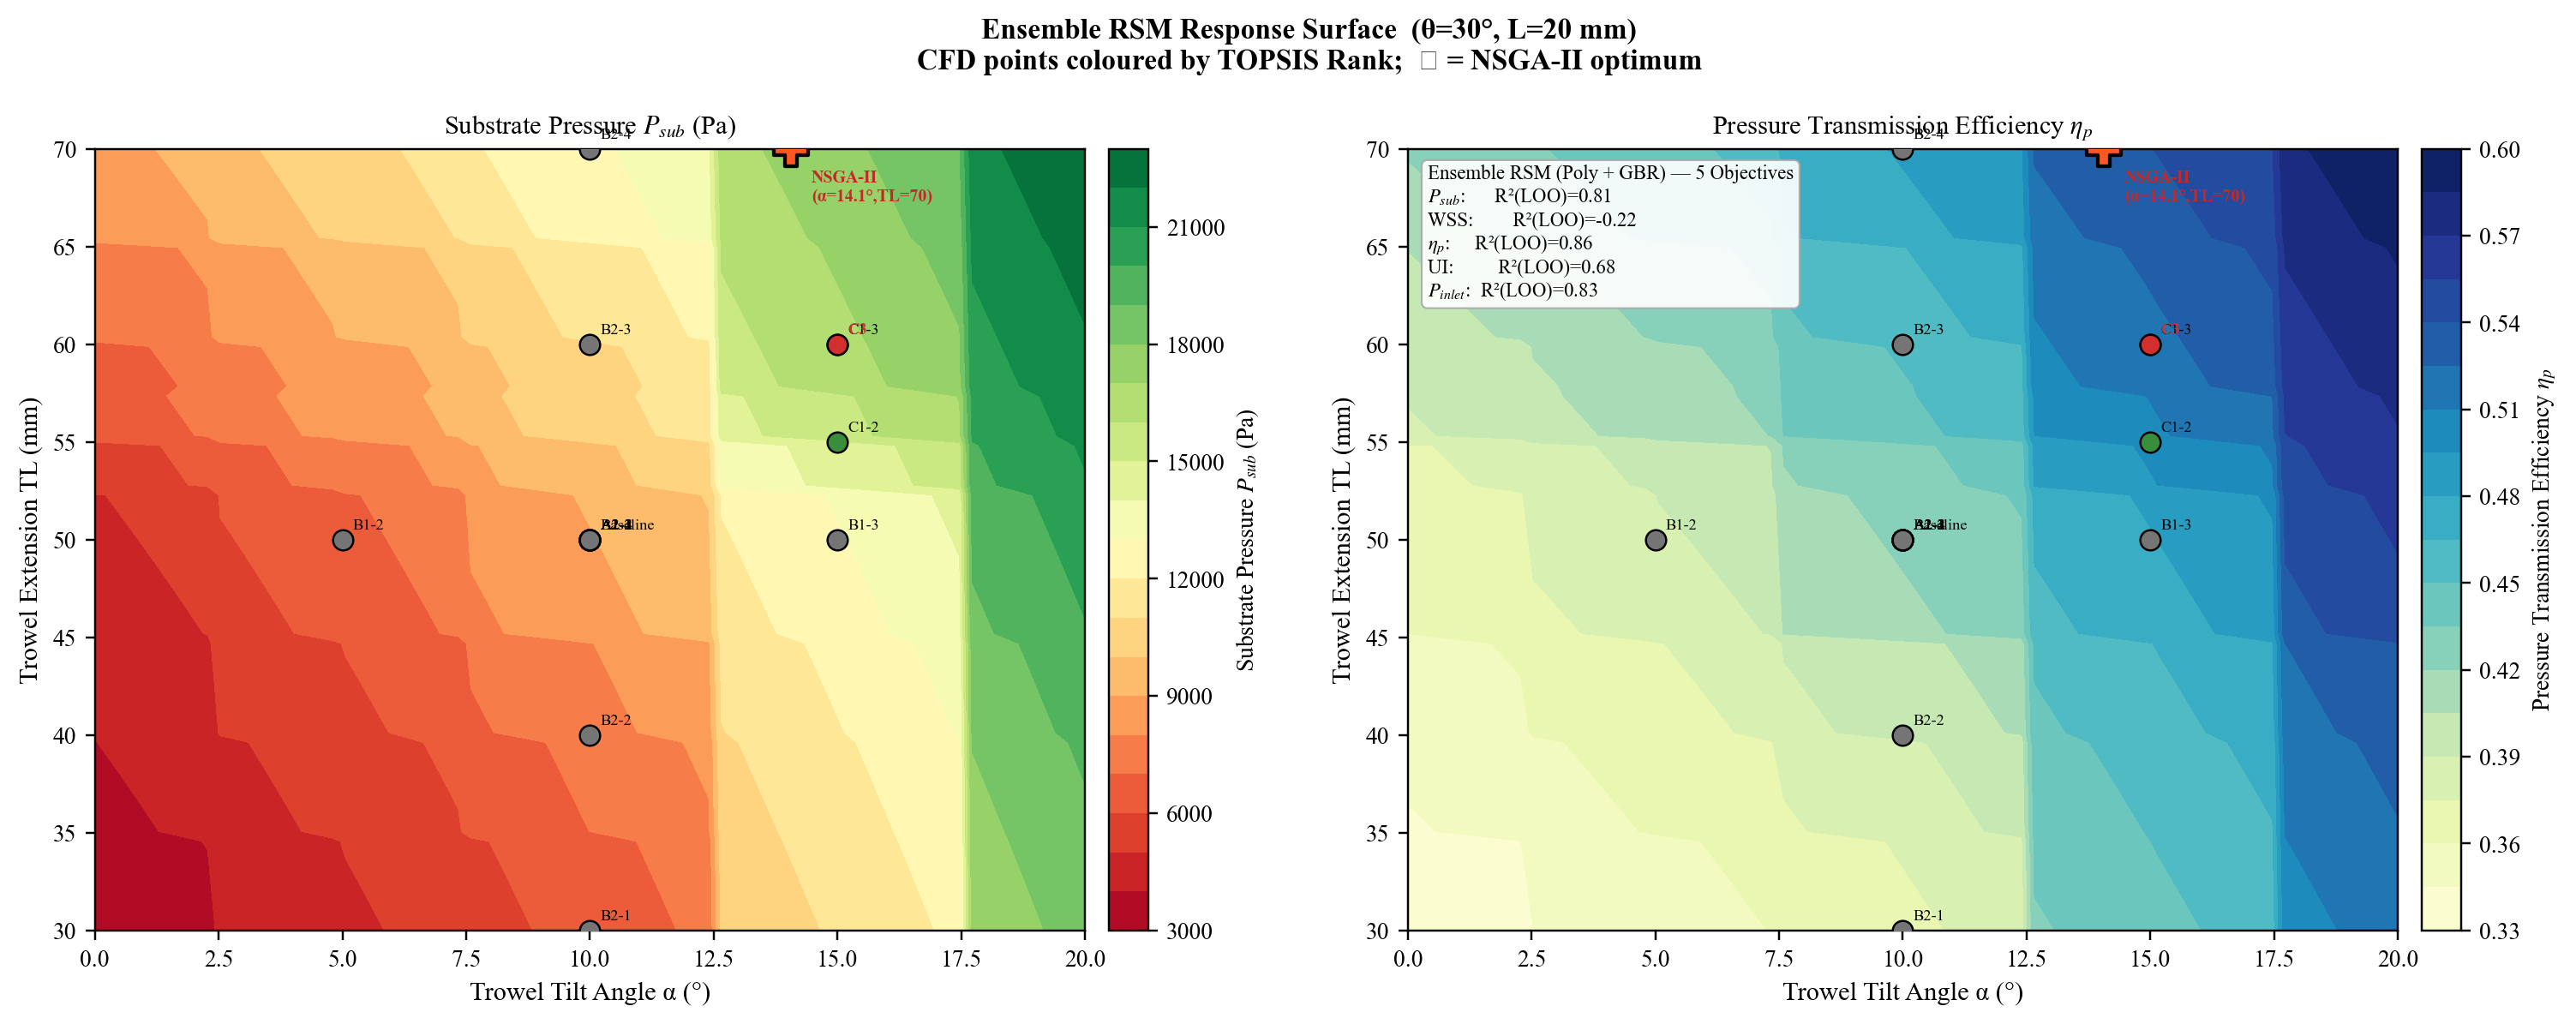
\includegraphics[width=0.95\textwidth]{figures/5.3.png}
  \caption{集成多项式RSM响应面（左）、CFD数据点与NSGA-II最优点（右）}
  \label{fig:5.3}
\end{figure}

\begin{table}[!htb]
  \centering
  \caption{代理模型LOO-CV结果汇总}\label{tab:5.3}
  \renewcommand{\arraystretch}{1.3}
  \begin{tabular}{lcccc}
    \toprule
    \textbf{目标} & \textbf{方法} & $R^2$(LOO) & \textbf{RMSE} & \textbf{可信度评级} \\
    \midrule
    $P_{sub,AWA}$    & Poly RSM & 0.815  & 2260.97 & 强 \\
    $WSS_{nozzle}$   & Poly RSM & -0.221 & 114.41  & 低 \\
    $\eta_p$         & Poly RSM & 0.860  & 0.03    & 较强 \\
    $UI$             & Poly RSM & 0.678  & 0.07    & 一般 \\
    $P_{inlet}$      & Poly RSM & 0.826  & 3102.29 & 较强 \\
    \bottomrule
  \end{tabular}
\end{table}

由结果可见，各目标代理模型的预测质量存在明显差异。$P_{sub,AWA}$的代理模型表现最好，说明代理模型能够较为可靠地捕捉基底压力随参数变化的趋势。$\eta_p$的代理模型质量居中，由于$\eta_p = P_{sub}/P_{inlet}$，其变化趋势与$P_{sub}$高度相关（$r = 0.962$），代理模型能够对其进行合理预测。

$WSS_{nozzle}$的代理模型质量最差，LOO-CV得到的$R^2$为负值，说明代理模型的预测能力甚至不及简单均值预测。这一异常结果的根本原因在于数据中存在严重的异常点：B1-1工况（$\alpha = 0°$）的$WSS_{nozzle} = 445.5$~Pa，约为其他工况平均值的5.6倍，这一极端值严重扭曲了代理模型的拟合，使模型既无法准确拟合正常工况，也无法正确预测异常工况。$UI$的代理模型同样表现较差，主要原因可能在于$UI$对几何参数的响应关系的复杂性，模型很难在17个数据点的条件下完整刻画4个主效应项和6个交叉项。

\subsection{模型局限性}

本课题建立的代理模型具有以下的局限性，需要在根据代理模型优化决策时慎重考虑：

（1）数据规模对泛化能力的限制。本研究仅有17个可行CFD工况，而代理模型需要在4维参数空间中进行插值与外推。数据点的分布遵循单因素变化原则，参数空间的``角落''（如高$TL$、高$\theta$、高$\alpha$的组合）缺乏直接CFD数据，代理模型在这些区域的预测可信度较低。

（2）$L$变量信息不足。Pearson相关分析已证明$L$对$P_{sub,AWA}$的影响在统计上不显著（$r = -0.038$，$p = 0.873$）。在代理模型中，$L$的变化几乎不改变任何目标函数的预测值，这意味着代理模型对$L$这个维度基本无感，NSGA-II在$L$方向的优化结果（$L = 40$~mm）本质上是在一个噪声主导的维度上搜索，物理意义有限，不宜据此对$L$参数作出工程推荐。

（3）$WSS_{nozzle}$代理模型不可用于定量预测。鉴于$WSS_{nozzle}$代理模型的负$R^2$，NSGA-II基于该模型对$WSS_{nozzle}$的优化结果仅具有方向性参考价值（即``更小的$\alpha$和$\theta$有利于降低WSS''的趋势），而不能作为绝对值预测的依据。

在后续对课题的深度研究和完善过程中，可以通过拉丁超立方抽样等的种种空间填充方法增加CFD工况，以提升代理模型的空间覆盖度，增加代理模型的可信度。

\section{TOPSIS综合排名}

\subsection{归一化加权评分方法}

在对17个可行工况进行综合排名时，采用TOPSIS（Technique for Order Preference by Similarity to Ideal Solution）思路的线性加权归一化评分方法。具体步骤为：将五个目标的实测值分别进行Min-Max归一化，使各目标均映射至$[0, 1]$区间，方向统一为归一化值越小越优，对于需要最大化的目标，归一化时取反；随后以等权重$w_i = 0.2$对归一化后的五个目标进行加权求和，得到复合评分：
\begin{equation}\label{eq:topsis}
  S_{composite} = \sum_{i=1}^{5} w_i \cdot f_i^{norm}, \quad w_i = 0.2.
\end{equation}
复合得分越小，表明该工况在五个目标上的综合表现越优。

此处等权重计算不同目标的决定，是在缺乏明确工程优先级信息的情况下对各目标不偏不倚的处理方式。但是在实际工程应用中，不同工程在不同时段会产生不同的目标与优先级，需要根据具体需求对权重进行调整。

\subsection{排名结果}

17个可行工况的TOPSIS综合排名结果见\cref{fig:5.4}与\cref{tab:5.4}。

\begin{table}[!htb]
  \centering
  \caption{TOPSIS工况排名表}\label{tab:5.4}
  \renewcommand{\arraystretch}{1.3}
  \begin{tabular}{ccccccccc}
    \toprule
    \textbf{排名} & \textbf{工况} & $TL$ & $\theta$ & $\alpha$ & $P_{sub,AWA}$ & $WSS_{nozzle}$ & $\eta_p$ & $UI$ \\
    \midrule
    1 & C3   & 60 & 60° & 15° & 21702 & 25.1  & 0.560 & 1.582 \\
    2 & C1-3 & 60 & 60° & 15° & 21677 & 41.1  & 0.557 & 1.585 \\
    3 & C1-2 & 55 & 30° & 15° & 14525 & 74.7  & 0.506 & 1.644 \\
    4 & B1-3 & 50 & 30° & 15° & 12081 & 77.1  & 0.481 & 1.645 \\
    5 & B2-4 & 70 & 30° & 10° & 12833 & 102.1 & 0.483 & 1.683 \\
    \bottomrule
  \end{tabular}
\end{table}

\begin{figure}[!htb]
  \centering
  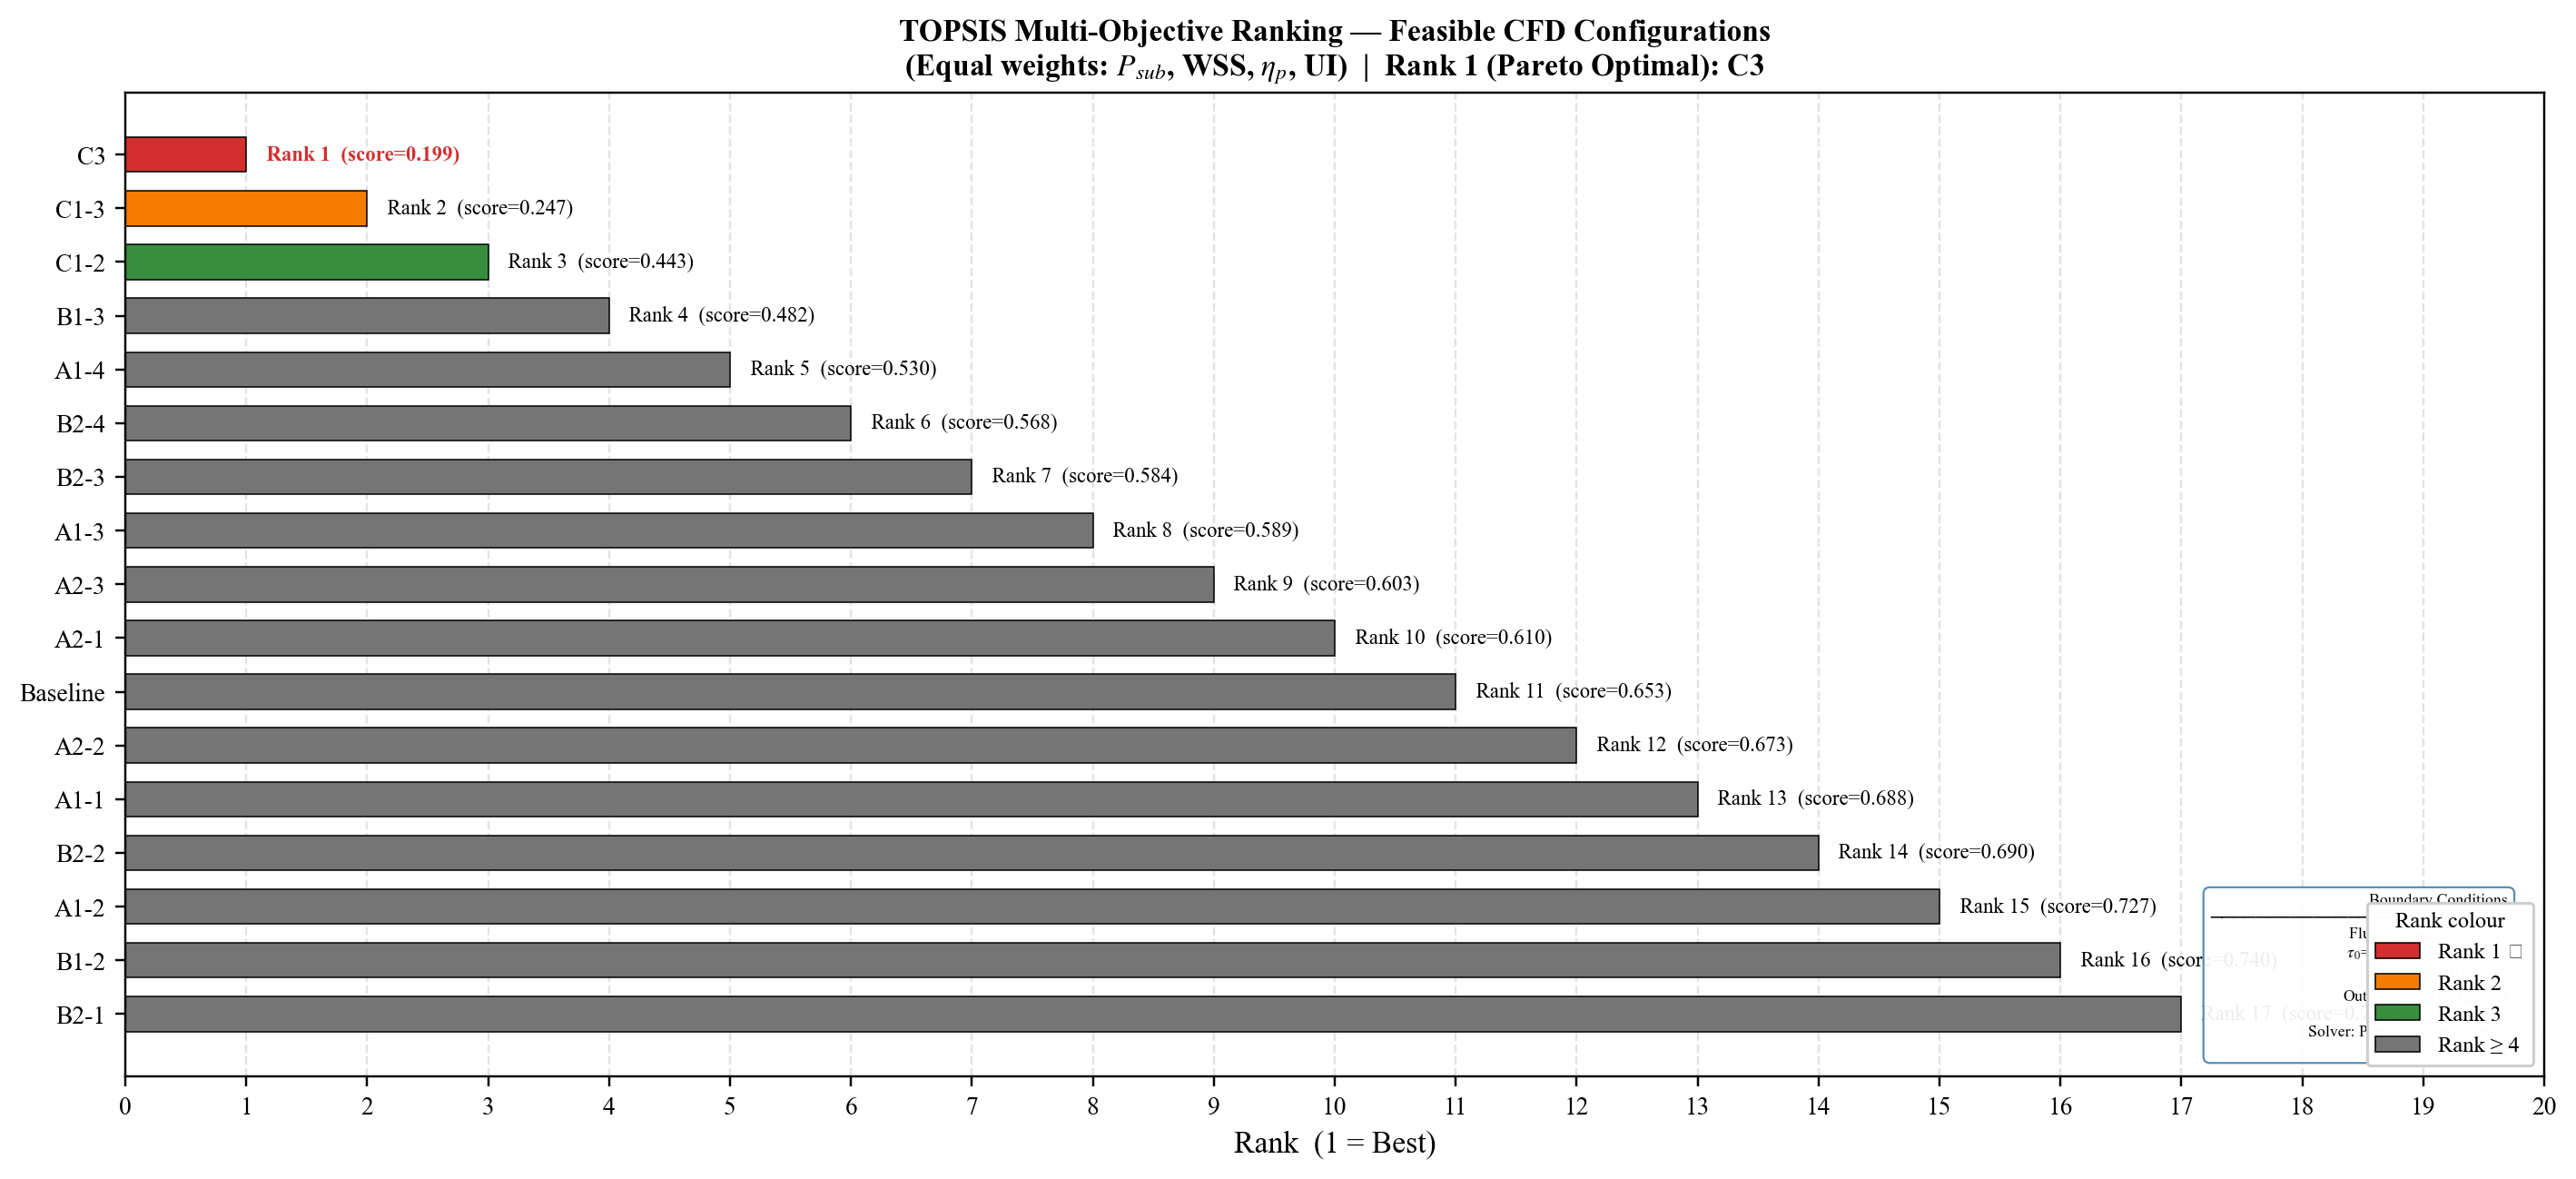
\includegraphics[width=0.8\textwidth]{figures/5.4.png}
  \caption{TOPSIS综合排名水平柱状图}
  \label{fig:5.4}
\end{figure}

C3工况（$TL = 60$~mm，$\theta = 60°$，$L = 20$~mm，$\alpha = 15°$，含Fillet）以复合得分0.000排名第一，是本研究在五目标等权重框架下的综合最优配置。C1-3工况紧随其后（$S = 0.059$），两者参数完全相同，仅几何倒角处理有所不同。C3对C1-3的优势集中体现在$WSS_{nozzle}$指标上（25.1 vs 41.1 Pa，降低39\%），在其他四个目标上两者几乎无差异（$P_{sub}$差异$<0.1\%$，$\eta_p$差异$<0.6\%$）。这再次说明：几何倒角虽然对宏观压力场影响微乎其微，但其对喷嘴近壁剪切状态的改善足以在五目标等权重评分中拉开差距，确立C3的综合最优地位。

第3-5名（C1-2、B1-3、B2-4）均包含$\alpha = 15°$或$TL \geq 60$~mm，也进一步印证了\cref{chap:parametric}参数重要性排序的结论，即$\alpha$和$TL$是对综合性能贡献最大的两个参数。排名靠后的工况（如A1-2、B1-2、B2-1等）共同特点是接触压力较低或$\eta_p$较小，说明在等权重评分下，接触压力维度的相对劣势难以被其他目标的优势所弥补。在实际工程运用中，排名与不同工况所产生的优势势必会随着权重与目标的不同而变化。

\section{Pareto Front支配分析}

\subsection{四目标Pareto Front分析}

Pareto支配分析是多目标优化中识别不可改进解的标准方法。若不存在任何其他可行解能够在所有目标上同时不差于该解、且至少在一个目标上严格优于该解，则称该解为Pareto最优解（Pareto-optimal solution），Pareto最优解的集合构成Pareto前沿。

在四目标框架（$f_1 = -P_{sub}$，$f_2 = WSS_{nozzle}$，$f_3 = -\eta_p$，$f_4 = UI$）下，对17个可行CFD工况进行穷举式Pareto支配判断，结果表明：C3是唯一的Pareto最优配置，在四维目标空间中不受任何其他工况的支配。

\cref{fig:5.5}展示了四对目标组合下的二维Pareto散点图。在所有子图中，C3均位于其他工况构成的散点群的前沿位置，直观验证了其Pareto最优性。

\begin{figure}[!htb]
  \centering
  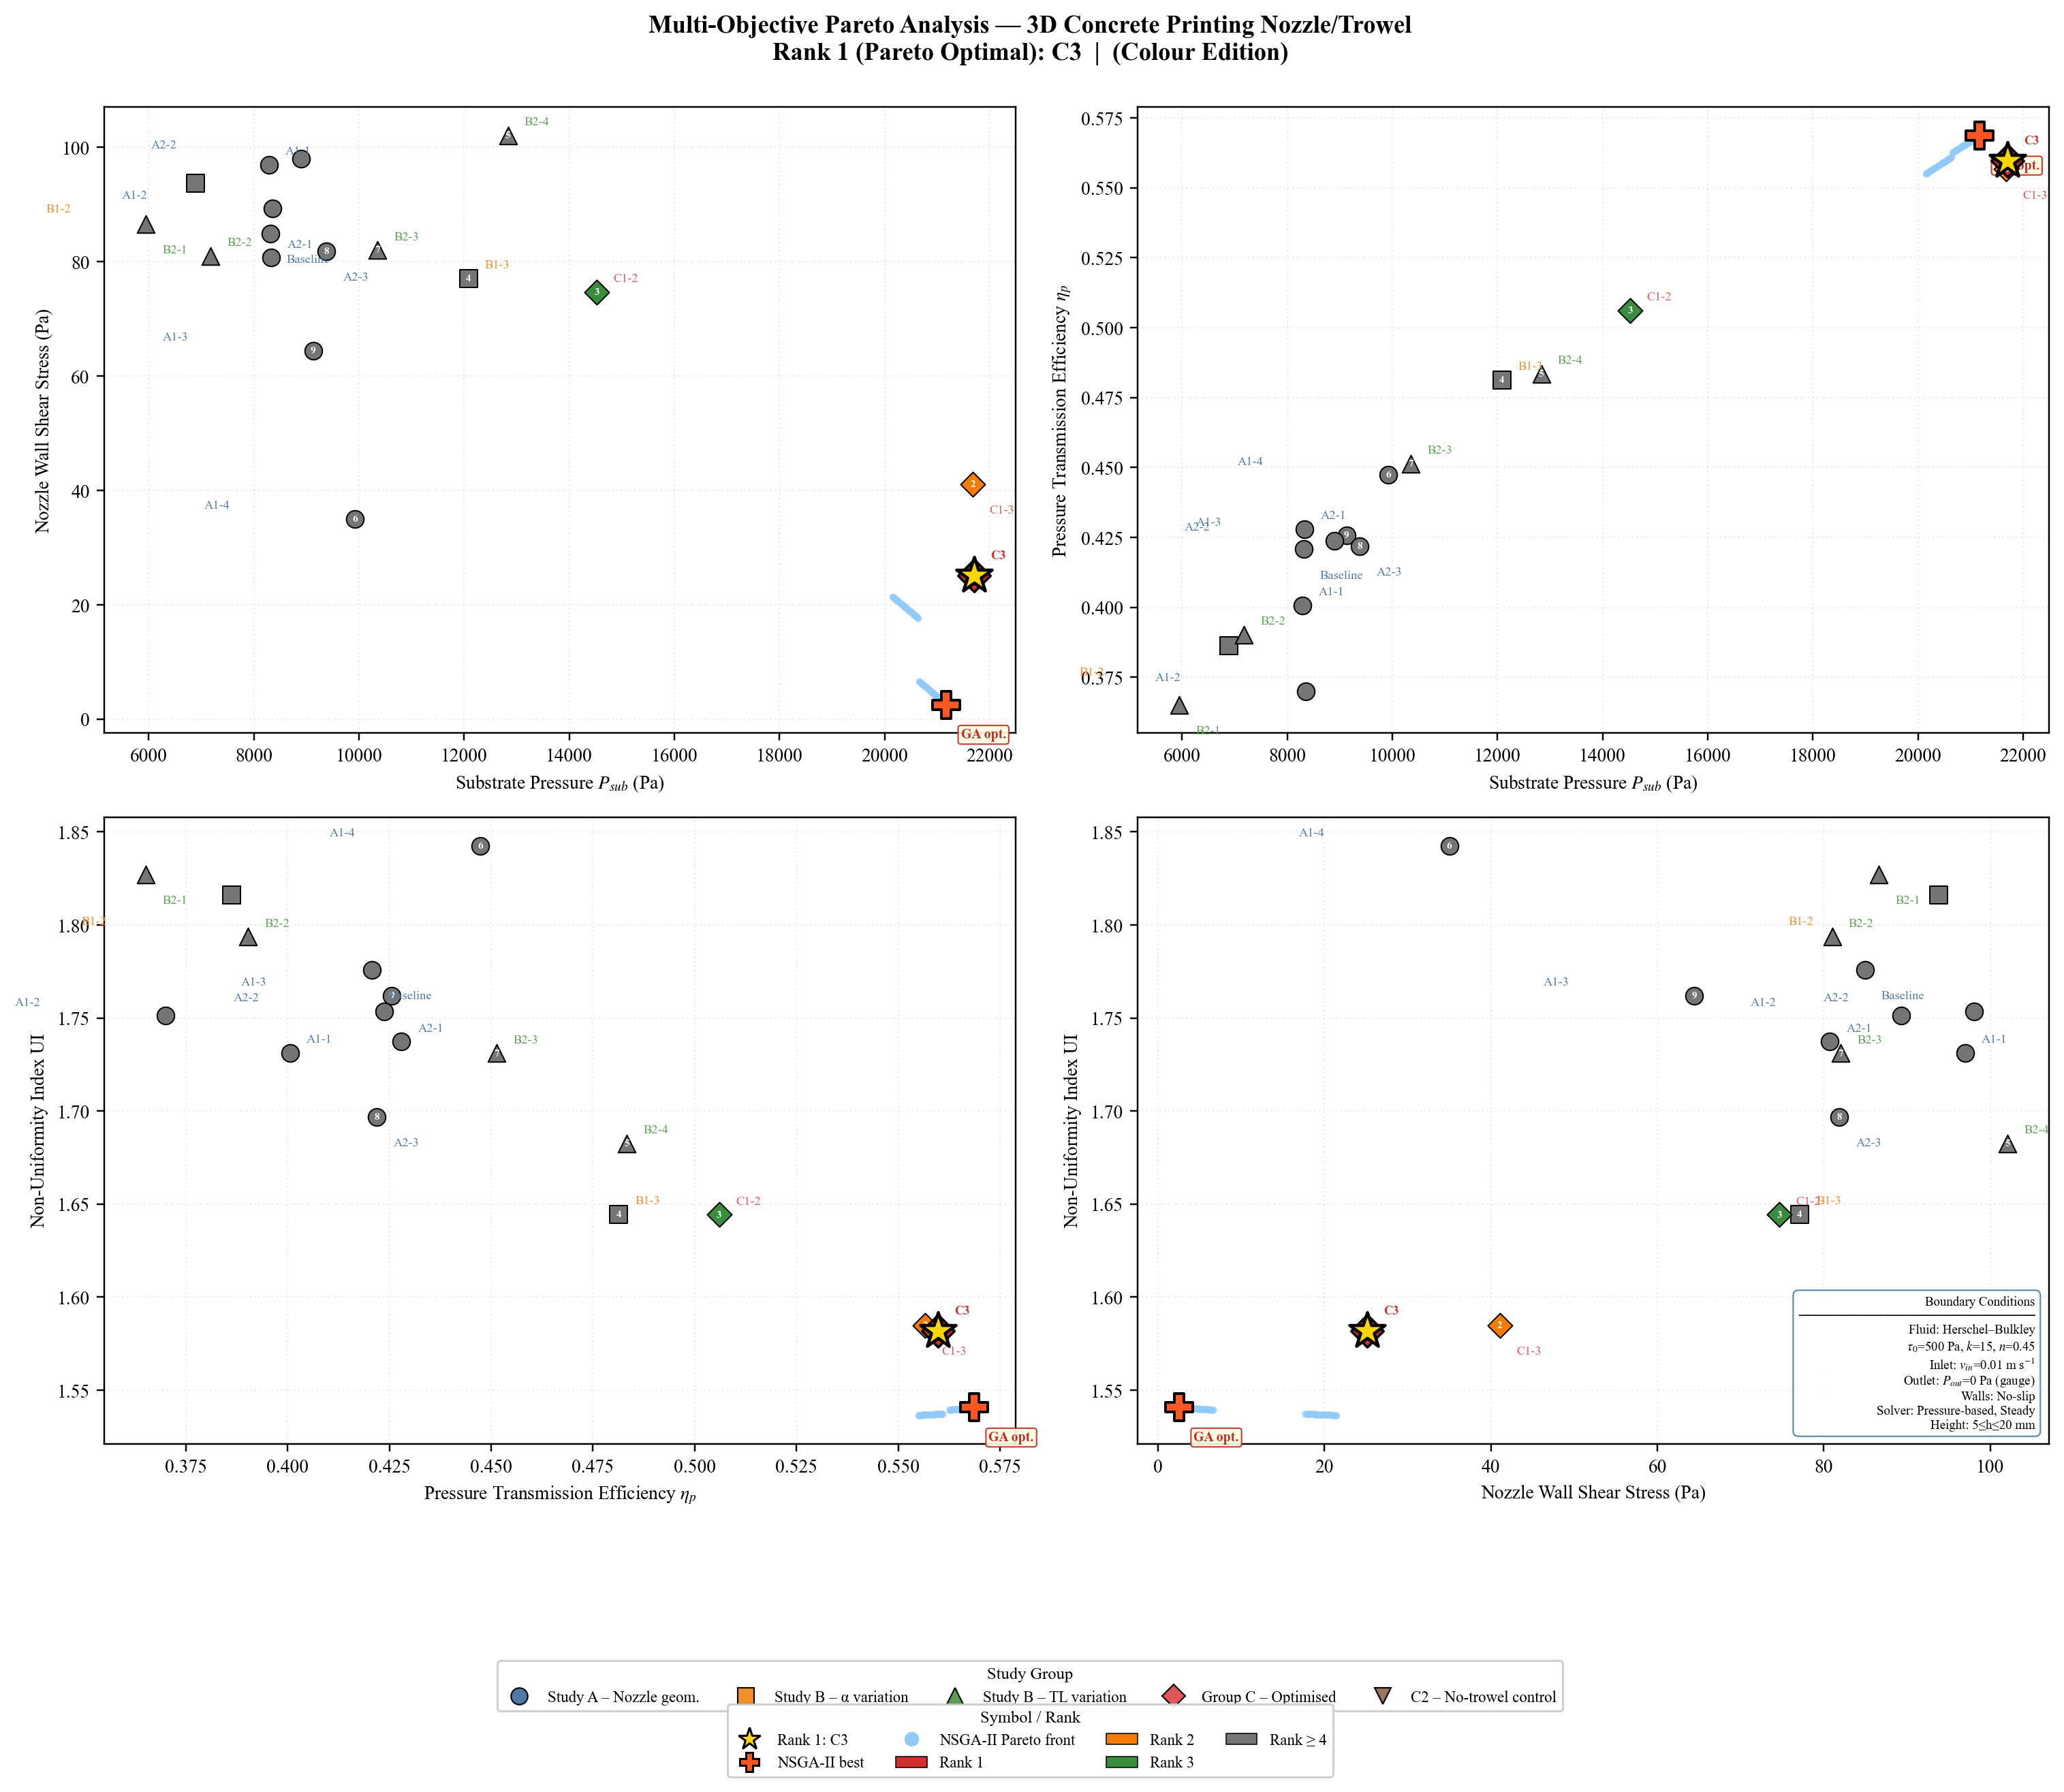
\includegraphics[width=0.95\textwidth]{figures/5.5.png}
  \caption{四目标Pareto散点图}
  \label{fig:5.5}
\end{figure}

次优工况C1-3在$P_{sub}$（21677 vs 21702 Pa，差0.1\%）、$\eta_p$（0.557 vs 0.560，差0.5\%）和$UI$（1.585 vs 1.582，差0.2\%）三个目标上与C3几乎无差异，但在$WSS_{nozzle}$（41.1 vs 25.1 Pa）上明显劣于C3，因此被C3严格支配。这一分析再次确认：在C1-3基础上增加几何倒角（C3）是一个严格的Pareto改进，在不损失任何其他目标性能的前提下，显著降低了喷嘴壁面剪切应力，体现了倒角作为几何优化手段的确定性价值。

\subsection{五目标Pareto Front分析与目标共线性}

将$P_{inlet}$纳入第五个优化目标后，Pareto格局发生了根本性变化：Pareto最优点从1个扩展至13个（占17个可行工况的76\%），大量低能耗工况（如B2-1、B1-2等）进入Pareto Front。最优点数量激增这一显著变化的根源在于$P_{inlet}$与$P_{sub,AWA}$之间的体现的高度共线性。20个CFD工况在$P_{inlet}$-$P_{sub,AWA}$散点图上的分布图如\cref{fig:5.6}所示。

\begin{figure}[!htb]
  \centering
  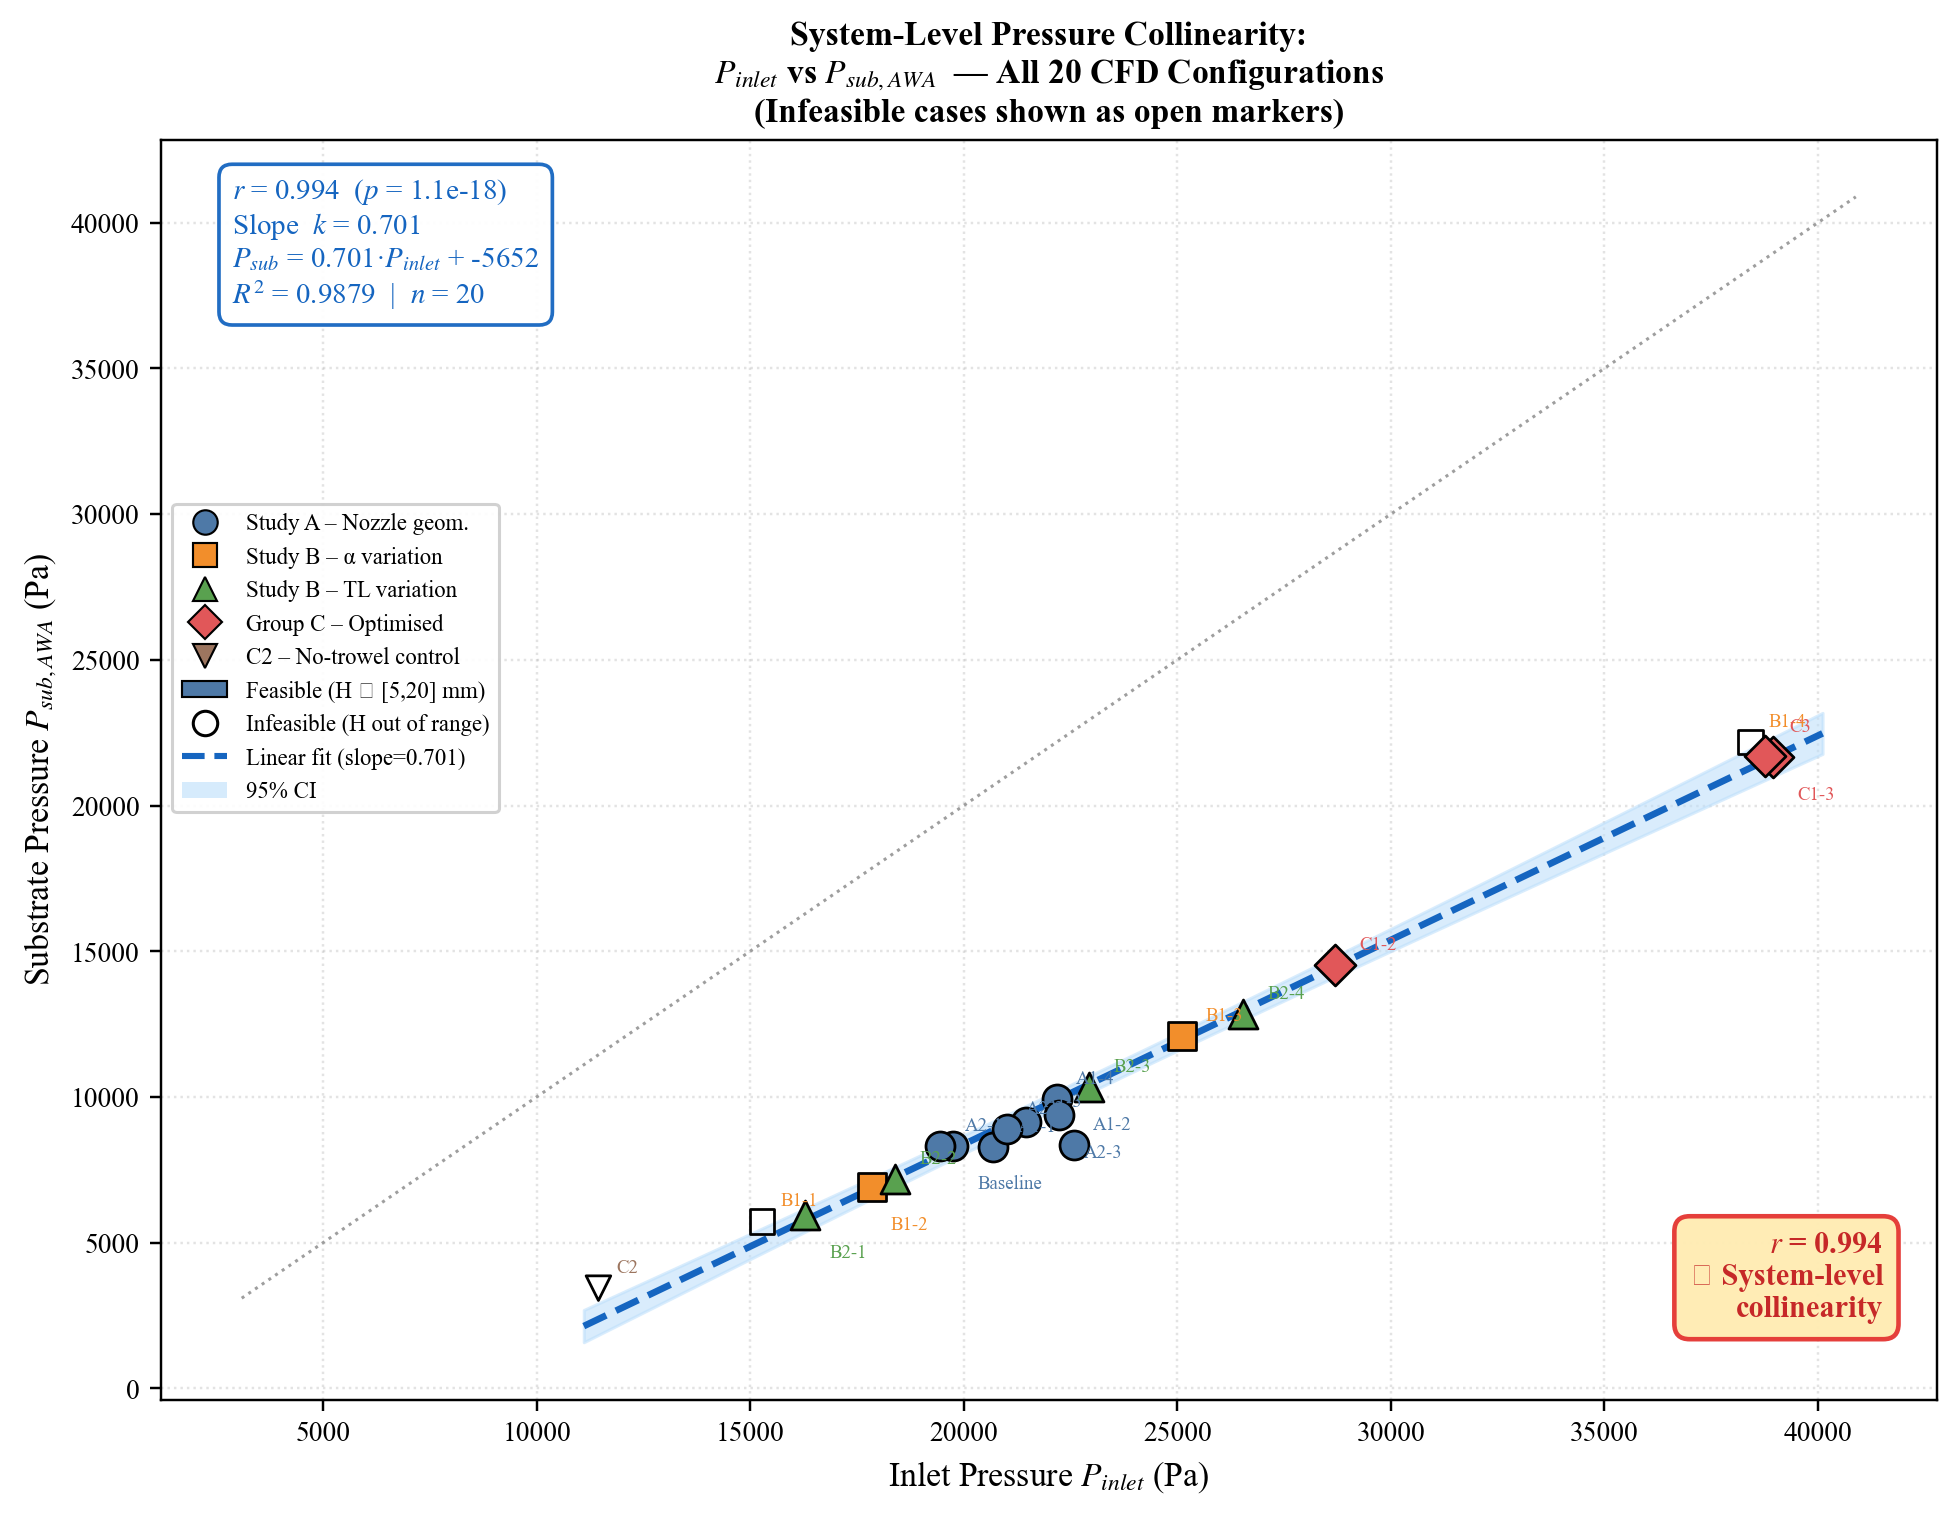
\includegraphics[width=0.75\textwidth]{figures/5.6.png}
  \caption{$P_{inlet}$--$P_{sub,AWA}$散点图}
  \label{fig:5.6}
\end{figure}

线性拟合结果表明：
\begin{equation}\label{eq:Pinlet-Psub}
  P_{inlet} \approx \frac{1}{\bar{\eta}_p} \cdot P_{sub,AWA} \approx 1.427 \cdot P_{sub,AWA},
\end{equation}
Pearson相关系数$r = 0.9879$（$p < 0.001$），20个工况的数据点几乎完美地排列在一条直线上。这一近乎确定性的线性关系揭示了本研究打印系统的一个基本物理规律：在当前喷嘴-整形板几何框架下，提升基底接触压力与增大泵送入口压力是等价的操作。系统的压力传递效率$\eta_p$在不同工况间的变异极小（约在0.37-0.58之间），几何参数的改变主要影响压力的绝对水平，而非传递效率本身。

\cref{tab:5.5}列出了主要目标对的Pearson相关系数。除$P_{inlet}$-$P_{sub}$的高度共线性外，结合\cref{fig:4.20}还可观察到：$\eta_p$与$P_{sub}$之间具有强正相关性（$r = 0.962$），而$UI$与$\eta_p$之间展现强负相关（$r = -0.901$）。这说明在本研究的参数空间内，五个目标并非独立，压实能力、剪切损伤、低能耗这三个目标基本涵盖了全部五个目标的信息。

\begin{table}[!htb]
  \centering
  \caption{主要目标对的Pearson相关系数表}\label{tab:5.5}
  \renewcommand{\arraystretch}{1.3}
  \begin{tabular}{lccccc}
    \toprule
                 & $P_{sub,AWA}$ & $WSS_{nozzle}$ & $\eta_p$ & $UI$    & $P_{inlet}$ \\
    \midrule
    $P_{sub,AWA}$  & 1.000  & -0.465 & 0.962  & -0.861 & 0.994  \\
    $WSS_{nozzle}$ & -0.465 & 1.000  & -0.534 & 0.629  & -0.518 \\
    $\eta_p$       & 0.962  & -0.534 & 1.000  & -0.901 & 0.953  \\
    $UI$           & -0.861 & 0.629  & -0.901 & 1.000  & -0.884 \\
    $P_{inlet}$    & 0.994  & -0.518 & 0.953  & -0.884 & 1.000  \\
    \bottomrule
  \end{tabular}
\end{table}

在五目标框架下，低接触压力但低泵送能耗的工况（如B2-1：$P_{sub} = 5944$~Pa，$P_{inlet} = 16277$~Pa）与高接触压力但高泵送能耗的工况（如C3：$P_{sub} = 21702$~Pa，$P_{inlet} = 38772$~Pa）处于同等的Pareto地位，因为两者各有所长，无法通过单一工况在所有五个目标上同时超越对方，而这也正是五目标分析所揭示的能耗-压实固有权衡关系的集中体现。工程师在实际打印系统设计中，需要根据泵送设备的压力能力和对层间粘结强度的具体要求，在Pareto Front上选取合适的工作点。

\section{NSGA-II多目标遗传算法优化}\label{sec:nsga2}

\subsection{NSGA-II算法设置}

NSGA-II（Non-dominated Sorting Genetic Algorithm II）是求解多目标优化问题的一种遗传算法，其核心特征是通过非支配排序与拥挤距离机制，在单次运行中同时生成分布均匀的Pareto Front近似解集，适合处理连续参数空间内的多目标工程优化问题。

本课题建立的NSGA-II遗传算法以建立多项式RSM代理模型作为目标函数评估器，每次函数评估的计算时间为毫秒量级，使算法能够在合理时间内完成$200 \times 300 = 60000$次函数评估。具体超参数设置见\cref{tab:5.6}。

\begin{table}[!htb]
  \centering
  \caption{NSGA-II算法参数设置}\label{tab:5.6}
  \renewcommand{\arraystretch}{1.3}
  \begin{tabular}{lll}
    \toprule
    \textbf{参数} & \textbf{设定值} & \textbf{说明} \\
    \midrule
    种群规模         & 200             & 4维参数空间覆盖 \\
    迭代代数         & 300             & 收敛性保证 \\
    交叉算子         & SBX             & 模拟二进制交叉 \\
    变异算子         & PM              & 多项式变异 \\
    随机种子         & 42              & 结果可重现 \\
    约束处理         & 惩罚函数        & 层高约束 $H \geq 5$~mm \\
    \bottomrule
  \end{tabular}
\end{table}

种群规模200能够为4维参数空间提供足够的多样性覆盖；模拟二进制交叉（SBX）和多项式变异（PM）是处理连续变量优化问题的标准算子；随机种子固定为42确保结果可重现；层高约束通过惩罚函数处理，对不满足$H \geq 5$~mm的个体施加大惩罚值，使其在非支配排序中被自动淘汰。这些关键设置可以保证NSGA-II在课题特定的五目标框架下发挥较优解析能力。

\subsection{NSGA-II Pareto Front结果}

\cref{fig:5.7}给出了NSGA-II生成的Pareto Front（约200个解）与17个CFD数据点在四对目标组合下的叠加图。

\begin{figure}[!htb]
  \centering
  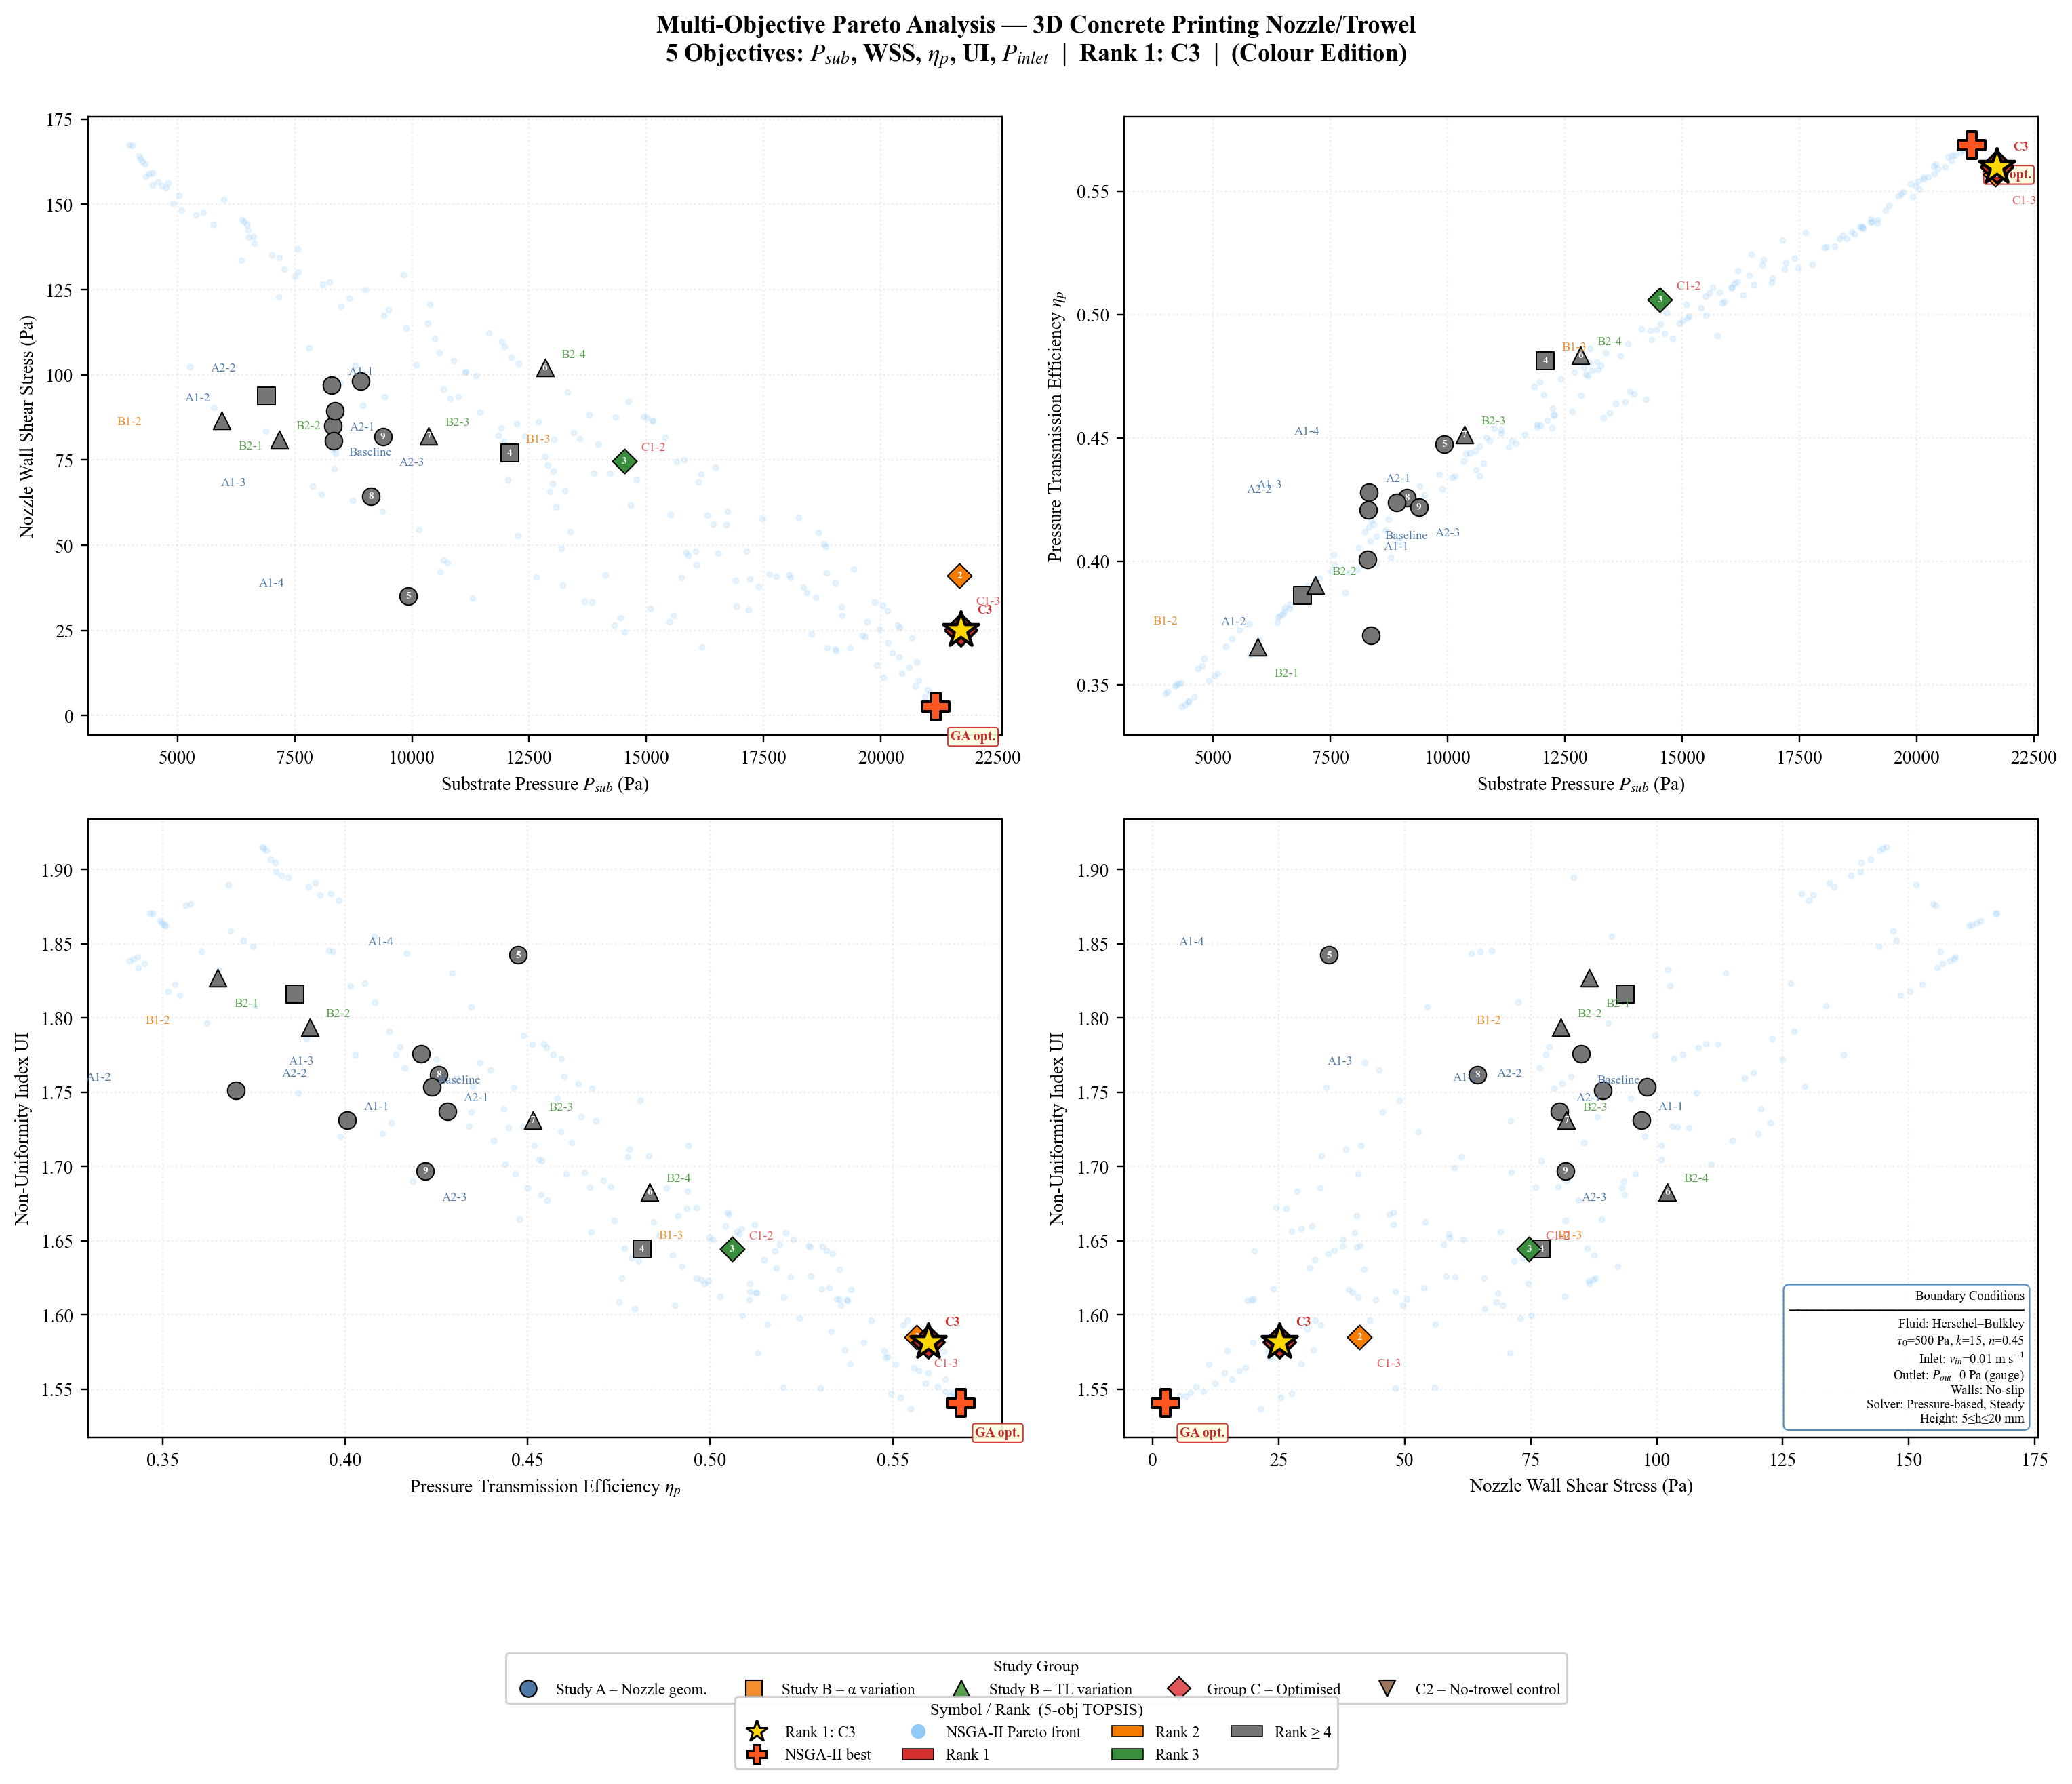
\includegraphics[width=0.95\textwidth]{figures/5.7.png}
  \caption{NSGA-II Pareto Front结果散点图}
  \label{fig:5.7}
\end{figure}

由图可见，NSGA-II生成的Pareto Front在$P_{sub}$-$WSS$和$P_{sub}$-$\eta_p$空间中均呈现出连续平滑的曲线形态，清晰展示了各目标之间的权衡关系：随着$P_{sub}$的提高，$WSS_{nozzle}$和$P_{inlet}$均呈上升趋势，而$\eta_p$则略有提升，$UI$略有下降。这与前叙的参数化研究的定性结论完全一致。

前沿解的参数分布同样具有重要的参考价值：在Pareto Front上，高性能端（高$P_{sub}$）的解具有普遍的倾向：
\begin{equation}\label{eq:pareto-pref}
  TL \to 70~\text{mm}, \quad \theta \to 60°, \quad \alpha \to \text{boundary optimum}.
\end{equation}
这与CFD单因素分析中各参数的最优方向完全吻合，从侧面验证了代理模型在方向性预测上的可靠性。尽管代理模型的绝对值预测精度有限，但它对参数影响方向的刻画是正确的。这种NSGA-II Pareto解集与单因素CFD分析之间的一致性，进一步证明了优化方向的可靠性。

\subsection{NSGA-II综合最优解}

由\cref{fig:5.3}所示的RSM响应面可见，在TOPSIS等权重评分（$w_i = 0.2$）下，对Pareto Front上的约200个解进行综合评分，确定最优设计参数为：$TL = 70$~mm，$\theta = 60°$，$L = 40$~mm，$\alpha = 14.06°$，对应层高$H = 22 - 70 \times \sin(14.06°) = 5.00$~mm。

该解处于层高约束的精确边界，揭示了一个重要的工程含义：在当前几何框架下，最大化综合性能的最优策略是将层高压缩至允许的最小值，充分利用楔形效应的压力增益，直至层高约束被激活。这种现象表明，层高下界$H_{min} = 5$~mm是制约进一步提升接触压力的根本约束。如果工程里接受更薄的沉积层，系统仍有进一步改善的空间；但是如果约束不可放宽，那么NSGA-II最优解代表了给定约束下的理论性能极限。

另外，NSGA-II给出的最优$L$值为40~mm。\cref{chap:parametric}Pearson相关分析已经证明$L$对$P_{sub}$的影响统计上不显著（$p = 0.873$），代理模型对$L$维度基本无法区分，所以这里给出的最优$L$值很可能是在噪声主导的目标函数中产生的伪结果，它不具有实质性的物理依据。

\subsection{NSGA-II验证工况CFD分析}

将NSGA-II最优解的参数设置放入同样环境配置的ANSYS Fluent软件中进行CFD模型模拟，其结果与C3工况的定量对比如\cref{tab:5.7}所示。\cref{fig:5.8}展示了五目标归一化雷达图的对比。

\begin{table}[!htb]
  \centering
  \caption{NSGA-II最优解与C3工况CFD结果对比}\label{tab:5.7}
  \renewcommand{\arraystretch}{1.3}
  \footnotesize
  \begin{tabular}{lccccccccc}
    \toprule
    \textbf{工况} & $TL$ & $\theta$ & $L$ & $\alpha$ & $P_{sub}$(Pa) & $WSS_{nozzle}$ & $\eta_p$ & $UI$ & $P_{inlet}$ \\
    \midrule
    Pareto Optimum & 70 & 60 & 40 & 14.06 & 43760 & 53.85 & 0.593 & 1.70 & 73844 \\
    C3             & 60 & 60 & 20 & 15    & 21702 & 25.13 & 0.560 & 1.58 & 38772 \\
    \bottomrule
  \end{tabular}
\end{table}

\begin{figure}[!htb]
  \centering
  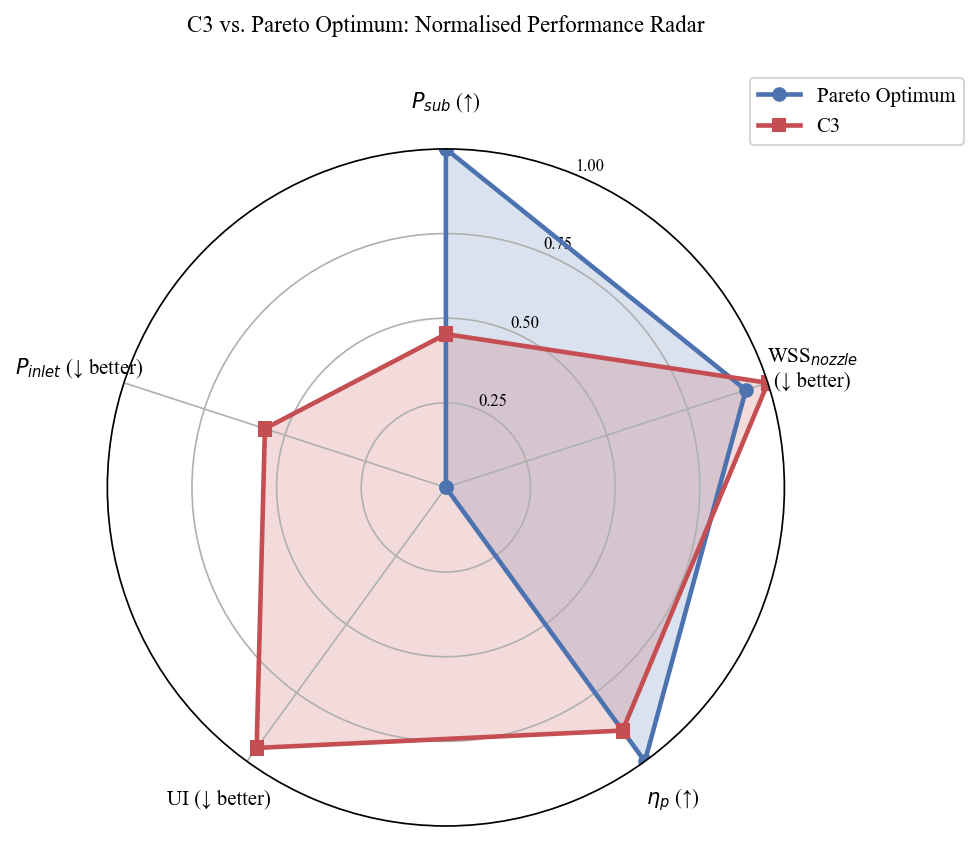
\includegraphics[width=0.7\textwidth]{figures/5.8.png}
  \caption{NSGA-II验证工况与C3对比雷达图}
  \label{fig:5.8}
\end{figure}

对比两项试验结果，有以下几个角度值得讨论：

（1）压实效果：NSGA-II最优工况的$P_{sub,AWA} = 43760$~Pa，较C3（21702~Pa）提升+102\%，几乎翻倍。这一巨大提升主要来自两方面：$\alpha = 14.06°$与$TL = 70$~mm将层高压缩至5~mm，楔形效应达到最大，且$TL$的增大进一步延长了约束路径，两者协同产生了极高的接触压力。

（2）泵送能耗：接触压力翻倍，泵送压力也近乎翻倍。NSGA-II最优工况的$P_{inlet} = 73844$~Pa，较C3（38772~Pa）增加+90\%，几乎同比例上升。结合\cref{eq:Pinlet-Psub}所揭示的$P_{inlet} \approx 1.42 \times P_{sub}$共线关系，可以完全解释这一现象。

（3）压力传递效率：NSGA-II最优工况的$\eta_p = 0.593$，较C3的0.560仅提升+5.9\%。这一结果说明最优工况花费90\%更多的泵送能耗，但是仅仅只能换来5.9\%的效率改善。从投入产出比的角度来看，追求比C3更高的接触压力的边际效益极低，工程代价极高。

（4）层高：NSGA-II最优工况是课题研究设置的最低值，而这个结果本身就会带来一定的不确定性：如果为了极限优化的其它目标而去压榨最终打印混凝土的层高，那么混凝土层高本身作为一个打印混凝土结果中重要的评价指标，它的不确定性将会大大增加。一旦出现材料流变性能波动或设备误差，极易导致整形板末端与已打印层发生接触，破坏打印质量。

综合以上分析可以得出：NSGA-II最优解代表了本研究参数范围内的理论压实极限，但其高达73844~Pa的泵送压力要求以及极小的层高余量，使其在工程实践中的可行性受到严格限制。C3工况（$P_{sub} = 21702$~Pa，$P_{inlet} = 38772$~Pa，$H = 6.47$~mm）在保持合理泵送压力和充足层高余量的前提下，实现了相对于基准工况161\%的压实提升，是综合性能与工程可靠性的最优平衡点，也是本研究推荐的工程实用方案。

\chapter{讨\quad 论}\label{chap:discussion}

\section{主要发现}

\subsection{喷嘴几何参数对打印性能的影响机制}

本研究系统考察了四个喷嘴与整形板几何参数（$\theta$、$L$、$TL$、$\alpha$）对基底接触压力及相关打印性能指标的影响，结果揭示了各参数作用机制的本质差异，为打印喷嘴的工程设计提供了清晰的物理背景。

\textbf{（1）喷嘴收缩角$\theta$的双重作用机制}

收缩角$\theta$通过两条相互独立的物理路径影响打印性能。其一是压力路径：较大的收缩角使流道截面积沿轴向更急剧地减小，浆体在收缩段内受到更强的径向压缩，出口截面动压更高，经前挡板阻挡后转化为更大的基底接触压力，为下游整形板区域提供更高的压力输入。其二是剪切路径：更大的收缩角使流线沿收缩壁面的曲率变化趋于平滑，抑制了收缩段转角处的流动分离，消除了局部高剪切速率集中区，有效降低壁面剪切应力。这两条路径的方向一致，赋予了收缩角参数独特的优化特征，在不引入任何指标劣化的前提下同时改善接触压力和剪切应力，具有重要的工程价值。

\textbf{（2）喷嘴竖直高度$L$的有限调控作用}

相比$\theta$和整形板参数，喷嘴竖直高度$L$对基底接触压力的影响最为有限。从流动的角度理解，喷嘴竖直高度的主要功能是为流体提供充分发展的速度剖面，保证进入下游收缩段的流动状态稳定，而非主动产生动压或楔形约束效应。延长直管段仅增加管道摩擦损失，对出口截面的速度分布和动压幅值几乎无影响，因而对基底接触压力的调控能力极弱。整形板末端剪切应力 $WSS_{outlet}$ 随$L$变化的先减后升则反映了竖直高度通过影响速度剖面充分发展程度而间接作用于整形板区域的局部流动状态，很可能属于二阶效应。综合来看，$L$在本文研究范围内是一个比较弱的影响参数，在满足制造约束的前提下，其具体取值对打印性能的影响可后置考虑。

\textbf{（3）整形板结构的不可替代性}

无顶板对照工况（C2）的CFD结果说明：去除整形板顶板后，多项指标成为全部工况中最低值，甚至低于无整形板的理论自由挤出状态。这一结果表明，整形板顶板并非简单的成形模具，而是产生基底接触压力的核心功能构件。其作用机制在于：顶板封闭了流体向上方逃逸的路径，将喷嘴出口的高动压流体强制约束在楔形通道内，使动能得以有效转化为作用于基底面的静压。一旦顶板缺失，流体以近乎无约束的方式向四周扩散，原本用于产生接触压力的动能大量耗散，导致整体接触压力大幅下降，也会导致整体挤出性能下降。

\textbf{（4）整形板参数协同效应}

C1-3工况的 $P_{sub,AWA}$ 提升幅度显著超过各单因素效果的线性叠加，揭示了喷嘴参数与整形板参数之间存在正向协同增强机制。$\theta=60°$的大收缩角使喷嘴出口流体具有更高的动压和更均匀的速度剖面，而$\alpha=15°$与$TL=60$~mm所形成的强楔形约束空间对高动压流体的压力转化效率更高。在这个体系下，输入动压越高，楔形效应产生的压力增益越大，两种效应的协同效应导致总压力增益超过各自独立贡献之和。这一协同机制的存在意味着，在实际打印系统优化中，喷嘴参数（$\theta$）与整形板参数（$\alpha$、$TL$）更应作为一个整体系统加以联合优化，而非独立调节。

\subsection{打印性能指标之间的耦合与权衡关系}

\textbf{（1）压实性能与泵送能耗的高度共线性}

全部20个工况的 $P_{inlet}$ 与 $P_{sub,AWA}$ 之间的Pearson相关系数高达 $r=0.994$（$p<0.001$），两者近乎完全共线，线性拟合关系为 $P_{inlet} \approx 1.77 \times P_{sub,AWA}$。这一发现揭示了当前喷嘴-整形板系统的一个根本性约束：提升层间压实效果与降低泵送能耗是相互对立的，在本课题的研究系统架构下无法独立解耦。本研究所采用的几何参数（$\theta$、$L$、$TL$、$\alpha$）均通过改变流动阻力来调控接触压力，而增大接触压力必然要求克服更大的流动阻力，更大的流动阻力直接体现为更高的入口驱动压力。这一内在耦合的存在，在五目标Pareto分析中导致 $P_{inlet}$ 与 $P_{sub,AWA}$ 成为近乎等价的目标维度，也就导致了完全共线的拟合关系。在工程实践中，若想要提高基底接触面的压力大小，则必须需要这必须在系统设计阶段预先考量泵送系统的工作压力限制，找到一个系统平衡点。

\textbf{（2）压实性能与剪切应力的条件性权衡}

在一般情况下，提升接触压力往往伴随着更强的流场约束和更大的速度梯度，导致壁面剪切应力升高，但本研究下喷嘴出口倾斜角度$\theta$同时实现了接触压力提升和壁面剪切应力降低。另外，倒角处理则提供了另一条打破常规权衡的途径：在不牺牲接触压力的前提下，通过消除尖角处的流动分离，倒角可以显著降低壁面剪切应力。因此，压实与剪切之间的权衡关系并非不可调和，而是取决于具体的几何优化手段。宏观喷嘴几何和局部转角几何均可在特定条件下同时改善两个目标。

\textbf{（3）Pareto Front的几何形态与设计含义}

在以最大化基底接触压力和最小化壁面剪切应力构成的二维目标空间中，CFD工况点的分布呈现出清晰的Pareto Front结构。C3工况位于四目标Pareto Front的唯一最优点，而C1-3仅因壁面剪切应力劣于C3而被支配。这一结构表明，在可行设计空间内，C3代表了当前参数组合下压实性能与剪切损伤控制的最优平衡点，继续改变任何单一参数均无法在不损失其他目标的前提下进一步改善综合性能。

NSGA-II在代理模型上搜索到的理论最优点（$TL=70$，$\theta=60°$，$\alpha=14.06°$，$H=5$~mm）虽然能将基底接触压力提升超过一倍，但其泵送压力也同步提升了一倍，压力传递效率 $\eta_p$ 仅仅只有微弱的提升，清晰地说明了在层高约束的硬性边界附近，继续追求极限压实性能的边际效益急剧下降，工程代价大幅上升，C3才是综合考量下最具工程实用价值的设计方案。

\subsection{层高约束对混凝土打印性能的主导效应}

在本研究的所有参数化发现中，\cref{eq:H}揭示的层高解析关系：
\begin{equation}
  H = Z_0 - TL \cdot \sin(\alpha) \tag{2.1}
\end{equation}
是贯穿全部结果的核心约束机制，其重要性远超单一几何参数的影响。从物理层面上来看，$\alpha$和$TL$对基底接触压力的影响并非独立的几何效应，而是两个共享同一物理中间量（混凝土层高 $H$）的耦合路径：$\alpha$增大通过增大 $\sin(\alpha)$ 来减小 $H$，$TL$增大通过增大前乘系数来放大 $\sin(\alpha)$ 的效果，两者都通过缩小出口间隙来增强Reynolds楔形压力，本质机制相同，只是调控路径不同。

这个约束具有重要的简化意义：在参数优化中，$\alpha$和$TL$并不是两个真正独立的自由度，而是在层高约束的框架下共同决定出口间隙高度的两个相关参数。当 $H$ 被固定时，$\alpha$和$TL$之间存在确定的几何替代关系，增大一个参数可以在保持 $H$ 不变的前提下等效替代另一个参数对接触压力的贡献。也正因如此，在NSGA-II的优化搜索中，$\alpha$和$TL$均趋向其各自的上界，共同将层高压缩至约束下界，这实际上正是层高约束作为主导变量主动锁定了最优解的位置。

如果要在确定$\alpha$和$TL$的基础上进一步提升接触压力而不受层高约束限制，有效的系统级改进路径有：增大提高喷嘴离地高度或减小 $H_{min}$。通过改进浆体配比提高早龄期强度，使更薄的沉积层仍能保持稳定，可能是打印混凝土性能提高的另一方向。

\section{工程设计建议}

综合参数化研究与多目标优化结果可知，不同几何参数对打印性能具有明显不同的作用机制。其中，整形板倾斜角 $\alpha$ 对基底接触压力的调控最为敏感，但同时会显著压缩层高余量；整形板长度 $TL$ 能够以较为线性且可预测的方式提升压实能力，同时对层高影响相对温和；收缩角 $\theta$ 在提高接触压力的同时，还能够显著降低喷嘴壁面剪切应力，表现出较好的协同优化特性。相比之下，而喷嘴竖向高度 $L$ 对整体性能影响较弱，在本研究范围内可视为次要参数。此外，转角圆角处理虽然对接触压力改善有限，但能够明显降低局部壁面剪切应力与潜在磨损风险，是一种具有较高工程性价比的优化措施。

综合五目标Pareto Front分析、TOPSIS排序以及流场结构分析结果，推荐采用C3工况作为最优设计方案，即 $\theta=60°$、$TL=60$~mm、$L=20$~mm、$\alpha=15°$，并在关键转角区域引入3--5~mm的圆角过渡处理。这个方案在保持可接受层高余量的同时，实现了较高的基底接触压力、较低的局部剪切损伤以及较优的压力传递效率。虽然入口压力同步增加约，但整体仍处于工程可接受范围内，表现出较优的综合打印性能。

\section{方法局限性讨论}

\subsection{CFD模型假设局限}

本研究的CFD模型建立在若干理想化假设基础上，以提高计算效率并控制参数复杂度，因此对真实3D打印混凝土过程的描述仍存在一定局限性。本课题采用稳态单相流模型，并没有考虑打印混凝土的触变性、结构重建以及多层沉积过程中的时变行为，而实际浆体的早龄期强度会随时间持续演化，并对层间稳定性与粘结性能产生重要影响。此外，模型将浆体视为均质连续介质，忽略了润滑层形成、骨料迁移及离析等多相流效应，这可能导致对壁面剪切应力和系统压降的预测偏高。

混凝土浆体在挤出时同样伴随着水化放热反应，但是CFD模拟假设等温条件与刚性光滑壁面，不仅无法模拟混凝土浆体水化热造成的温度变化，也无法模拟壁面粗糙度与磨损对流场的影响。另外，喷嘴出口与基底面之间的高度$Z_0$也是影响混凝土挤出性能的一大影响因素，在本研究中保持固定，其对接触压力与层高分布的独立影响尚未展开系统研究。未来工作可进一步引入触变性本构模型与瞬态多层打印模拟，以更全面地描述实际混凝土打印过程中的复杂流变行为与结构演化机制。

\subsection{代理模型精度局限}

本研究使用17个可行CFD工况数据点构建了4维多项式RSM代理模型，用于NSGA-II多目标优化搜索。2阶多项式RSM在4个设计变量下展开后包含15个基函数项，17个数据点仅提供了2个自由度用于残差估计，模型处于近过拟合状态，LOO交叉验证的预测误差必然偏大，泛化能力有限。在后续完善中，可以试图补充CFD数据点到45--70个，以便代理模型能够正常收敛，输出更加精准的预测值。

\subsection{实验验证缺失}

本研究为纯数值模拟研究，所有结论均基于CFD计算结果，尚缺乏实验室尺度打印试验的物理验证，这会导致模型预测结果在绝对数值层面存在一定的不确定性。打印混凝土的流变参数对模拟结果具有较高敏感性，本文采用的Herschel--Bulkley参数来源于文献中的典型打印混凝土数据，与实际材料配合比之间可能存在差异，这种差异可能进一步影响接触压力、壁面剪切应力以及系统压降的预测精度。

另外，基底接触压力在实验条件下较难直接测量，目前尚缺乏成熟且统一的测试方法，这也限制了本文关键评价指标的实验验证。未来工作可结合实验室打印平台，对代表性喷嘴工况开展入口压力、流量以及沉积形态等方面的对比测试，从而进一步评估本文CFD模型的工程适用性与预测可靠性。

\chapter{结论与展望}\label{chap:conclusion}

\section{主要结论}

本研究建立了含整形板的挤出式3D打印混凝土喷嘴三维CFD模型，针对喷嘴与整形板的4个几何参数，对20个工况进行了系统参数化分析，并构建了五目标Pareto Front分析与NSGA-II优化框架。主要结论如下：

\textbf{（1）模型可靠性}

基于Herschel--Bulkley本构关系建立的非牛顿流体CFD模型通过了网格无关性验证和质量守恒检验（所有工况误差$<1\%$），具备良好的数值可信度。

\textbf{（2）参数重要性排序}

整形板倾斜角对基底接触压力的影响最为显著，整形板长度次之；喷嘴收缩角在显著提升压力的同时还能降低喷嘴壁面剪切应力，具有双重优化效果，而喷嘴竖向高度的影响在统计上并不显著，在实际工程运用中可在工程范围内灵活选取。

\textbf{（3）综合最优配置}

在课题研究构建的几何系统下，C3配置（$TL=60$~mm，$\theta=60°$，$L=20$~mm，$\alpha=15°$）在本研究的离散工况中表现出最优综合性能，TOPSIS综合排名第一。相较于基准工况，其基底压力提升161\%，喷嘴壁面剪切应力降低70\%，压力传递效率$\eta_p=0.560$，混凝土层高$H=6.47$~mm，满足工程层高要求并留有安全余量，是本研究推荐的工程最优方案。

\textbf{（4）能耗与压实的共线性}

在课题研究构建的几何系统下，入口压力与基底压力具有高度共线性。这表明在该类约束流动系统中，提升压实效果伴随泵送能耗的比例增加，两者无法独立优化。这一系统级特性是进行打印参数设计时需要特地权衡的内在约束。

\textbf{（5）NSGA-II优化与边际效益}

经CFD验证的NSGA-II最优解（$TL=70$~mm，$\theta=60°$，$\alpha=14.06°$，$H=5.0$~mm）的基底压力达较C3提升一倍左右，但入口压力同步提升一倍，压力传递效率$\eta_p$仅提升5.9\%。最优解恰好落在层高约束下界，揭示了进一步提升压实效果的边际收益极低，C3是兼顾性能与能耗的工程平衡点。

\section{创新点}

\textbf{（1）建立了含完整整形板结构的三维CFD模型}

本课题首次将顶板、侧挡板与倾斜出料段纳入统一计算域，系统揭示了整形板几何参数对基底接触压力的影响机制。

\textbf{（2）构建了五目标Pareto Front分析与NSGA-II优化框架}

本课题将压力、剪切、效率、均匀性、能耗五个目标进行联合优化，发现入口压力与基底压力存在强共线性，为打印系统的能耗-压实协同设计提供了定量依据。

\section{未来工作展望}

尽管本文建立了基于CFD与代理模型的3D打印混凝土喷嘴优化框架，并获得了若干具有工程意义的结论，但仍存在进一步扩展与完善的空间。

首先，本文采用稳态Herschel--Bulkley模型描述浆体流变行为，尚未考虑材料沉积后的触变性与结构重建过程。未来工作可引入包含结构建立参数的触变性本构模型，并结合瞬态求解方法，对多层打印过程中的早龄期强度演化、层间稳定性以及结构变形行为进行更深入研究。此外，本研究中喷嘴离地高度 $Z_0$ 保持固定，其对接触压力分布与层高形成的独立影响尚未系统量化，后续可围绕不同 $Z_0$ 工况开展进一步参数化分析。

另一方面，本文所有结果均基于数值模拟，尚缺乏实验室打印测试的物理验证。未来可结合实际打印平台，对代表性喷嘴工况开展入口压力、流量及沉积形态等方面的实验对比，以进一步评估CFD模型的预测精度与工程适用性。同时，当前代理模型训练数据规模仍然有限，部分目标函数的预测能力有待提高，后续可通过扩充CFD工况数量与参数覆盖范围，进一步提升NSGA-II优化结果的可靠性。除此之外，未来还可将优化变量从几何参数拓展至材料流变参数，实现喷嘴结构设计与材料配比之间的协同优化。


% ============================================================
%  参考文献
% ============================================================
\makereferences

% ============================================================
%  附录
% ============================================================
\appendix
\appendixsection{全部工况完整CFD数据表}\label{sec:appendix-cfd-data}

本附录提供本研究全部20个CFD工况的完整数值结果数据，包括几何参数、层高以及五项核心评价指标，作为正文中各章节分析的完整数据支撑。

\appendixsubsection{20工况完整参数矩阵与组别说明}

\cref{tab:appendix-case-params}~汇总了全部CFD工况的设计变量、层高及组别说明。

\begin{table}[!htb]
  \caption{工况完整参数矩阵与组别说明表}\label{tab:appendix-case-params}
  \centering
  \zihao{-5}
  \begin{tabular}{@{}lcccccc@{}}
    \toprule
    工况 & $TL$ & $\theta$ & $L$ & $\alpha$ & $H$ & 组别说明 \\
         & (mm) & (°)      & (mm) & (°)    & (mm) &          \\
    \midrule
    Baseline     & 50 & 30 & 20 & 10    & 13.32 & 基准工况 \\
    \midrule
    A1-1         & 50 & 15 & 20 & 10    & 13.32 & 研究线A1：$\theta$变化 \\
    A1-2         & 50 &  0 & 20 & 10    & 13.32 & \\
    A1-3         & 50 & 45 & 20 & 10    & 13.32 & \\
    A1-4         & 50 & 60 & 20 & 10    & 13.32 & \\
    \midrule
    A2-1         & 50 & 30 & 10 & 10    & 13.32 & 研究线A2：$L$变化 \\
    A2-2         & 50 & 30 & 30 & 10    & 13.32 & \\
    A2-3         & 50 & 30 & 40 & 10    & 13.32 & \\
    \midrule
    B1-1         & 50 & 30 & 20 &  0    & 22.00 & 研究线B1：$\alpha$变化 \\
    B1-2         & 50 & 30 & 20 &  5    & 17.64 & \\
    B1-3         & 50 & 30 & 20 & 15    &  9.06 & \\
    B1-4$^*$     & 50 & 30 & 20 & 20    &  4.90 & \\
    \midrule
    B2-1         & 30 & 30 & 20 & 10    & 16.79 & 研究线B2：$TL$变化 \\
    B2-2         & 40 & 30 & 20 & 10    & 15.05 & \\
    B2-3         & 60 & 30 & 20 & 10    & 11.58 & \\
    B2-4         & 70 & 30 & 20 & 10    &  9.85 & \\
    \midrule
    C1-1         & 50 & 60 & 20 & 10    & 13.32 & C组：A组最优 \\
    C1-2         & 55 & 30 & 20 & 15    &  7.77 & C组：Trowel优化 \\
    C1-3         & 60 & 60 & 20 & 15    &  6.47 & C组：性能最优 \\
    C2           &  0 & 30 & 20 & --    & 22.00 & C组：无顶板对照组 \\
    C3           & 60 & 60 & 20 & 15    &  6.47 & C组：含Fillet几何优化 \\
    \midrule
    Pareto Opt.  & 70 & 60 & 40 & 14.06 &  5.00 & Pareto最优解 \\
    \bottomrule
  \end{tabular}

  \vspace{0.5em}
  \begin{flushleft}
  \zihao{-5}
  注：$^*$~B1-4工况层高$H=4.90$~mm$<5$~mm，违反层高约束（式\ref{eq:dH-dalpha}对应约束），\\
  在Pareto优化分析中作为不可行工况处理，但其CFD计算结果仍保留作为$\alpha=20°$时的极限对照数据。
  \end{flushleft}
\end{table}


\appendixsubsection{面积加权平均静压完整数据}

\cref{tab:appendix-pressure-awa}~列出了全部工况在各关键截面处的面积加权平均静压。

\begin{table}[!htb]
  \caption{工况面积加权平均静压汇总表（单位：Pa）}\label{tab:appendix-pressure-awa}
  \centering
  \zihao{-5}
  \begin{tabular}{@{}lccccc@{}}
    \toprule
    工况 & Inlet & Outlet & Nozzle Outlet Plane & Trowel Outlet Plane & Substrate \\
    \midrule
    Baseline     & 19749.91  & $-6.56\times10^{-1}$ & 13535.61 &  9114.39 &  8310.47 \\
    A1-1         & 20685.29  & $-5.06\times10^{-1}$ & 13321.88 &  9151.33 &  8286.46 \\
    A1-2         & 22584.25  & $-7.82\times10^{-3}$ & 13645.84 &  8998.82 &  8357.26 \\
    A1-3         & 21450.59  & $-7.78\times10^{-2}$ & 15764.66 &  9747.29 &  9130.13 \\
    A1-4         & 22189.69  & $0$                  & 17274.11 & 10556.72 &  9925.97 \\
    A2-1         & 19445.99  & $-1.28\times10^{-1}$ & 13389.67 &  9031.00 &  8322.72 \\
    A2-2         & 21016.55  & $-1.06\times10^{-1}$ & 14935.50 &  9499.63 &  8905.36 \\
    A2-3         & 22239.07  & $-5.96\times10^{-4}$ & 15319.47 & 10385.79 &  9382.45 \\
    B1-1         & 15274.27  & $-8.10\times10^{-1}$ &  5693.16 &  5880.20 &  5733.26 \\
    B1-2         & 17856.09  & $-2.39\times10^{-2}$ & 12111.65 &  7194.97 &  6896.39 \\
    B1-3         & 25100.53  & $-6.32\times10^{-3}$ & 19170.26 & 13572.16 & 12081.38 \\
    B1-4$^*$     & 38418.42  & $-2.06\times10^{-1}$ & 32233.50 & 26550.06 & 22184.38 \\
    B2-1         & 16277.09  & $-3.49\times10^{-1}$ & 10444.73 &  7199.89 &  5943.92 \\
    B2-2         & 18389.89  & $-7.02\times10^{-2}$ & 12131.11 &  8257.66 &  7176.85 \\
    B2-3         & 22937.20  & $-3.16\times10^{-1}$ & 17021.72 & 10593.06 & 10353.37 \\
    B2-4         & 26549.15  & $-7.46\times10^{-2}$ & 20724.94 & 12641.92 & 12833.41 \\
    C1-1         & 22189.69  & $0$                  & 17274.11 & 10556.72 &  9925.97 \\
    C1-2         & 28703.58  & $-1.548$             & 22836.05 & 15904.42 & 14524.77 \\
    C1-3         & 38942.11  & $0$                  & 33927.75 & 23498.43 & 21677.26 \\
    C2           & 11445.53  & $-2.84\times10^{-1}$ &  3562.46 &  8562.89 &  3436.09 \\
    C3           & 38772.20  & $0$                  & 33924.87 & 22933.57 & 21702.46 \\
    Pareto Opt.  & 73843.81  & $-2.75\times10^{-14}$& 66748.04 & 69632.73 & 43760.24 \\
    \bottomrule
  \end{tabular}
\end{table}


\appendixsubsection{基底面压力统计与壁面剪切应力完整数据}

\cref{tab:appendix-wss}~列出了全部工况基底面静压的最大值、最小值与平均值，以及喷嘴出口截面和Trowel出口截面的面积加权平均壁面剪切应力。

\begin{table}[!htb]
  \caption{工况基底面压力统计及壁面剪切应力汇总表}\label{tab:appendix-wss}
  \centering
  \zihao{-5}
  \begin{tabular}{@{}lccccc@{}}
    \toprule
    \multirow{2}{*}{工况} &
    \multicolumn{3}{c}{基底面静压（Pa）} &
    \multicolumn{2}{c}{壁面剪切应力 $WSS$（Pa）} \\
    \cmidrule(lr){2-4}\cmidrule(lr){5-6}
     & 最大值 & 最小值 & 平均值 & Nozzle出口截面 & Trowel出口截面 \\
    \midrule
    Baseline     & 13982.66 &  $ -775.27$ &  4907.38 &  84.93 & 172.73 \\
    A1-1         & 13968.28 &  $ -378.04$ &  5215.21 &  96.98 & 188.27 \\
    A1-2         & 14127.74 &  $ -507.12$ &  5115.34 &  89.30 & 193.07 \\
    A1-3         & 15981.61 &  $ -104.66$ &  5548.38 &  64.41 & 126.71 \\
    A1-4         & 17858.02 &  $ -429.54$ &  6121.29 &  35.00 &  96.43 \\
    A2-1         & 13795.51 &  $ -663.71$ &  5007.53 &  80.70 & 202.23 \\
    A2-2         & 15483.30 &  $ -133.97$ &  5426.34 &  98.06 & 118.85 \\
    A2-3         & 15658.86 &  $ -261.52$ &  5510.88 &  81.86 & 178.01 \\
    B1-1         & 10436.67 &  $ -223.61$ &  3796.24 & 445.49 & 244.25 \\
    B1-2         & 12184.07 &  $ -339.33$ &  4483.57 &  93.78 & 153.86 \\
    B1-3         & 19501.28 &  $ -366.62$ &  6740.50 &  77.09 & 191.88 \\
    B1-4$^*$     & 32922.00 &  $ -586.25$ & 11330.01 &  91.67 & 436.91 \\
    B2-1         & 10671.90 &  $ -188.32$ &  3778.39 &  86.59 & 120.71 \\
    B2-2         & 12480.22 &  $ -392.77$ &  4537.87 &  81.00 & 261.82 \\
    B2-3         & 17706.43 &  $ -215.33$ &  6228.29 &  82.02 & 274.67 \\
    B2-4         & 21089.00 &  $ -505.50$ &  7441.50 & 102.07 & 284.96 \\
    C1-1         & 17858.02 &  $ -429.54$ &  6121.29 &  35.00 &  96.43 \\
    C1-2         & 23185.38 &  $ -697.43$ &  8278.20 &  74.66 & 382.89 \\
    C1-3         & 34195.39 &  $ -160.91$ & 11740.54 &  41.07 & 429.32 \\
    C2           &  6237.96 &  $ -932.83$ &  2222.35 & 382.18 &  52.21 \\
    C3           & 34233.94 &  $ -98.30 $ & 13165.63 &  25.13 & 560.18 \\
    Pareto Opt.  & 68119.00 &  $-2659.24$ & 22925.43 &  53.85 & 495.54 \\
    \bottomrule
  \end{tabular}
\end{table}


%% ============================================================
\appendixsection{全部工况网格质量完整汇总表}\label{sec:appendix-mesh-quality}

\appendixsubsection{网格质量统计}

\cref{tab:appendix-mesh}~汇总了全部CFD工况的网格质量统计数据，包括最大长宽比、最大/最小面面积、最大/最小单元体积、总体积及最小正交性质量等关键指标。所有工况的网格质量均满足CFD数值计算的基本要求（最小正交性质量$>0.15$，最大长宽比$<20$），保证了求解过程的稳定性与计算结果的可靠性。

\begin{table}[!htb]
  \caption{全部工况网格质量汇总表}\label{tab:appendix-mesh}
  \centering
  \zihao{-5}
  \begin{tabular}{@{}lccccccc@{}}
    \toprule
    工况 & Max AR & Max Face (m$^2$) & Min Face (m$^2$) & Max Vol. (m$^3$) & Min Vol. (m$^3$) & Total Vol. (m$^3$) & Min Orth. Q \\
    \midrule
    Baseline     & 14.922 & 7.77E-05 & 2.29E-09 & 1.92E-07 & 6.12E-14 & 3.16E-04 & 0.203 \\
    A1-1         & 15.739 & 7.54E-05 & 4.37E-09 & 1.98E-07 & 7.86E-14 & 2.19E-04 & 0.204 \\
    A1-2         & 16.996 & 7.44E-05 & 6.45E-10 & 2.00E-07 & 2.39E-14 & 1.61E-04 & 0.160 \\
    A1-3         & 14.215 & 8.72E-05 & 1.76E-09 & 2.84E-07 & 3.80E-14 & 4.73E-04 & 0.206 \\
    A1-4         & 17.028 & 1.37E-04 & 1.95E-09 & 5.01E-07 & 8.15E-14 & 8.72E-04 & 0.177 \\
    A2-1         & 13.700 & 7.40E-05 & 1.94E-09 & 1.90E-07 & 3.64E-14 & 2.13E-04 & 0.201 \\
    A2-2         & 16.337 & 9.01E-05 & 1.99E-09 & 2.81E-07 & 5.17E-14 & 4.30E-04 & 0.201 \\
    A2-3         & 18.358 & 1.36E-04 & 2.63E-09 & 4.30E-07 & 6.74E-14 & 5.84E-04 & 0.202 \\
    B1-1         & 16.591 & 8.23E-05 & 2.71E-09 & 2.17E-07 & 7.89E-14 & 3.51E-04 & 0.215 \\
    B1-2         & 17.435 & 8.46E-05 & 1.72E-09 & 2.49E-07 & 3.69E-14 & 3.33E-04 & 0.170 \\
    B1-3         & 12.969 & 8.72E-05 & 2.18E-09 & 2.63E-07 & 6.82E-14 & 2.98E-04 & 0.219 \\
    B1-4         & 16.407 & 8.41E-05 & 1.94E-09 & 1.54E-07 & 4.33E-14 & 2.81E-04 & 0.200 \\
    B2-1         & 15.166 & 6.62E-05 & 1.95E-09 & 1.84E-07 & 4.35E-14 & 3.14E-04 & 0.211 \\
    B2-2         & 14.556 & 7.10E-05 & 2.48E-09 & 1.81E-07 & 6.82E-14 & 3.15E-04 & 0.202 \\
    B2-3         & 16.083 & 9.91E-05 & 2.47E-09 & 2.95E-07 & 6.96E-14 & 3.15E-04 & 0.201 \\
    B2-4         & 19.780 & 1.03E-04 & 2.40E-09 & 3.22E-07 & 6.81E-14 & 3.14E-04 & 0.207 \\
    C1-1         & 17.028 & 1.37E-04 & 1.95E-09 & 5.01E-07 & 8.15E-14 & 8.72E-04 & 0.177 \\
    C1-2         & 15.756 & 8.83E-05 & 2.14E-09 & 2.44E-07 & 5.25E-14 & 2.96E-04 & 0.203 \\
    C1-3         & 16.059 & 1.67E-04 & 2.45E-09 & 6.37E-07 & 7.16E-14 & 8.49E-04 & 0.205 \\
    C2           & 13.436 & 7.06E-05 & 2.61E-09 & 1.73E-07 & 7.41E-14 & 3.07E-04 & 0.218 \\
    C3           & 16.287 & 1.18E-04 & 6.56E-10 & 4.64E-07 & 9.53E-15 & 8.50E-04 & 0.204 \\
    Pareto Opt.  & 17.351 & 2.52E-05 & 6.46E-10 & 3.18E-08 & 7.68E-15 & 2.53E-03 & 0.215 \\
    \bottomrule
  \end{tabular}

  \vspace{0.5em}
  \begin{flushleft}
  \zihao{-5}
  注：所有工况均采用统一的5~mm全局网格尺寸 + 关键区域局部加密（边缘0.5--1~mm）+ Inflation边界层（5层，增长比1.2）策略，\\
  以保证各工况间结果的可比性。Pareto验证工况额外检查了切向偏斜度（Tangent Skewness），最大值为3.25，处于可接受范围。
  \end{flushleft}
\end{table}


\appendixsubsection{网格无关性验证完整数据}

\cref{tab:appendix-mesh-independence}~列出了§2.3.4节中针对C3工况进行的网格无关性验证的完整数据。

\begin{table}[!htb]
  \caption{C3工况网格无关性验证完整数据}\label{tab:appendix-mesh-independence}
  \centering
  \begin{tabular}{@{}cccccl@{}}
    \toprule
    网格尺寸 & 最大长宽比 & $P_{sub,AWA}$ & 与3 mm误差 & 评级 \\
    (mm)    & (Max AR)  & (Pa)          & (\%)       &      \\
    \midrule
    12.9 & 16.29 & 21702 & 2.5\% & 粗网格，通过 \\
    8.0  & 17.35 & 21503 & 3.5\% & 合格 \\
    5.0  & 16.59 & 22090 & 0.8\% & \textbf{推荐网格} \\
    3.0  & 15.44 & 22273 & ---   & 参考基准 \\
    1.0  & 17.93 & 22579 & 1.4\% & 曲面振荡，不采用 \\
    \bottomrule
  \end{tabular}
\end{table}

综合考虑计算精度与计算效率，本研究最终选定5~mm为全局网格尺寸。20个参数化工况均采用与C3验证工况相同的网格策略，确保各工况间结果的可比性。


% ============================================================
%  谢辞（取消章编号，页码继续）
% ============================================================
\backmatter
\chapter*{谢辞}
\addcontentsline{toc}{chapter}{谢辞}

——我还没写——


\end{document}
